\documentclass[12pt, oneside]{book} 

\usepackage{amscd}
\usepackage{amsmath}
\usepackage{amssymb}
\usepackage{amsthm}
\usepackage{verbatim}

\usepackage[utf8]{inputenc}
\usepackage{geometry}

\geometry{letterpaper}

\usepackage[pdftex]{graphicx}

\usepackage{setspace}
\usepackage{physics}
\usepackage[T1]{fontenc}
\usepackage[polish]{babel}
\usepackage{subcaption}
\usepackage[numbers]{natbib}
\usepackage{pdfpages}
\usepackage{bm}
\usepackage{listings}
\usepackage{todonotes}
\usepackage[section]{placeins}
\usepackage{caption}
\usepackage{color, colortbl}
\usepackage{rotating}

\setlength{\parindent}{0pt}
\setlength{\textwidth}{6.5in}
\setlength{\textheight}{8.5in}
\setlength{\oddsidemargin}{0pt}
\setlength{\evensidemargin}{0pt}
\setlength{\topmargin}{0pt}
\setlength{\marginparsep}{0pt}
\setlength{\marginparwidth}{1in}

\usepackage{array}
\usepackage{xassoccnt}

\newcolumntype{L}{>{\arraybackslash}m{11cm}}

\captionsetup[table]{name=Tabela}

\usepackage{fancyhdr}
\newcommand{\changefont}{
    \fontsize{9}{11}\selectfont
}
\fancyhf{}
\fancyhead[RE,LO]{\changefont \slshape \leftmark} 

\fancyfoot[C]{\thepage}



\makeatletter

\let\latex@@addcontentsline\addcontentsline 

\AtBeginDocument{%
    \renewcommand{\addcontentsline}[3]{%
  \def\@@zzz{#1}\def\@@zxx{lol}
  \latex@@addcontentsline{%
    \ifx\@@zzz\@@zxx lof\else #1\fi
  }{#2}{#3}%
}

\renewcommand\lstlistingname{Rysunek}
\let\l@lstlisting\l@figure
\let\c@lstlisting\c@figure
\let\thelstlisting\thefigure
\let\ftype@lstlisting\ftype@figure
}
\makeatother

\addto\captionspolish{
\renewcommand{\listtablename}{Spis tabel}
}

\begin{document}

\begin{titlepage}
\begin{center}

\vspace*{2cm}

{\huge \textbf{Rozprawa Doktorska}}
\vspace{2cm}

{\huge Rozproszony algorytm analizy cyberbezpieczeństwa w sieci korporacyjnej}

\vspace{2cm}

{\large Mgr inż. Michał Walkowski}


\begin{flushright}
\vspace{2cm}
{Promotor\\Profesor dr hab. inż.\\ Sławomir Sujecki}

\vspace{0.5cm}
{Promotor pomocniczy\\Dr inż. Jacek Oko}
\end{flushright}

\vfill

\vspace*{3cm}

POLITECHNIKA WROCŁAWSKA\\
Wydział Informatyki i Telekomunikacji\\
17 stycznia 2022
\end{center}
\end{titlepage}

\frontmatter 
\onehalfspacing

\chapter{Streszczenie}
Niniejsza rozprawa poświęcona jest ostatnio dynamicznie rozwijającej się dziedzinie teleinformatyki, jaką jest cyberbezpieczeństwo. W pracy skoncentrowano się na procesie zarządzania podatnościami, a w szczególności na metodach, które pozwalają na poprawienie bezpieczeństwa sieci teleinformatycznej poprzez udoskonalenie procesu priorytetyzacji podatności, wykorzystując wiedzę o monitorowanym środowisku.

\bigbreak
W rozprawie zaproponowane zostały metody automatycznej priorytetyzacji podatności z wykorzystaniem ogólnodostępnych standardów oceny krytyczności oraz informacji o wadze zasobu z punktu widzenia organizacji. Celem pracy jest wyznaczenie grupy podatności krytycznych, wysokich oraz średnich, jak również określenie kolejności, w jakiej powinny one być naprawiane poprzez dodanie kroku w fazie definiowania działań naprawczych procesu zarządzania podatnościami. Dodatkowo w pracy zostały ujęte mechanizmy pozwalające na wykonywanie obliczeń dla przyrastającej ilości danych z wykorzystaniem metod skalowania dostępnych w nowoczesnych technologiach rozwoju oprogramowania.

\bigbreak
Analiza uzyskanych wyników oraz badania przeprowadzone w rzeczywistych środowiskach teleinformatycznych potwierdziły przydatność zaproponowanych algorytmów. Ponadto, zaproponowano dalsze kierunki badań w zakresie analizy bezpieczeństwa oraz monitoringu badanych sieci korporacyjnych, przy wykorzystaniu informacji o znanych podatnościach.

\vspace*{1cm}
\textbf{Słowa kluczowe:} proces zarządzania podatnościami, znane podatności, bezpieczeństwo infrastruktury teleinformatycznej.

\chapter{Summary}
This dissertation is devoted to the dynamically developing field of ICT, which is cybersecurity. The work focuses on the vulnerability management process, in particular on methods that allow to improve the security of the ICT network by improving the vulnerability prioritization process, using knowledge regarding the monitored environment.

\bigbreak
The dissertation proposes methods of automatic vulnerability prioritization implementing the   generally available standards of criticality assessment and information regarding the importance of the asset from the organisation point of view. The aim of the work is to identify a group of critical, high and medium vulnerabilities that should be repaired in the first instance by adding an additional step in the phase of defining corrective actions in the vulnerability management process. In addition, the work includes mechanisms that allow to perform calculations for an increasing amount of data using scaling methods available in modern software development technologies.

\bigbreak
The analysis of the obtained results and the research carried out in real ICT environments confirmed the usefulness of the proposed algorithms. In addition, further research directions were proposed in the field of security analysis and monitoring of the investigated corporate networks with the use of information on known vulnerabilities.

\vspace*{1cm}
\textbf{Keywords:} vulnerability management process, known vulnerabilities, security of ICT infrastructure.

\chapter{Podziękowania}



\begin{flushleft}
\vspace{1cm}
\emph{Składam serdeczne podziękowanie Panom \\
Prof. dr hab inż. Sławomirowi Sujeckiemu oraz \\
Dr inż. Jackowi Oko za stałą opiekę oraz \\
stworzenie warunków do realizacji założeń naukowych.
}

\vspace{1cm}
\emph{Dziękuję mojej Dziewczynie Agacie oraz Mamie Wiolettcie\\
za wspieranie mnie przez cały okres pracy nad doktoratem,}

\vspace{1cm}
\emph{Dziękuję kolegom, w szczególności Marcinowi Jaroszewskiemu, \\
Maciejowi Nowakowi, Maciejowi Krakowiakowi oraz Konradowi Kałużnemu}

\vspace{1cm}
\emph{Dziękuję wszystkim niewymienionym, którzy wnieśli wkład\\
w powstanie tej pracy.}
\end{flushleft}

\chapter*{}
\pagestyle{empty}
Lista artykułów opublikowanych w trakcie realizacji pracy doktorskiej:
\begin{enumerate}
    \item {\emph{Referat konferencyjny}\newline
    Michał Walkowski, Jacek Oko, Sławomir Sujecki, Stanisław Kozdrowski\newline
    \textbf{The impact of cyber security on the quality of service in optical networks.}\newline
    Service Computation 2018 : The Tenth International Conferences on Advanced Service Computing [Dokument elektroniczny] : Barcelona, Spain, February 18-22, 2018 / eds. Arne Koschel, Janusz Klink, Andreas Hausotter. [B.m.] : IARIA, cop. 2018. s. 53-56.}
    \item {\emph{Referat konferencyjny} \newline
    Michał Walkowski, Maciej Biskup, Agata Szewczyk, Jacek Oko, Sławomir Sujecki\newline
    \textbf{Container based analysis tool for vulnerability prioritization in cyber security systems.}\newline
    2019 21st International Conference on Transparent Optical Networks (ICTON) / eds. Marek Jaworski, Marian Marciniak. Danvers, MA : IEEE ; Warsaw : National Institute of Telecommunications, cop. 2019. s. 1-4.}
    \item {\emph{Artykuł} - Punktacja z wykazu MNiSW: 100\newline
    Michał Walkowski, Maciej Krakowiak, Jacek Oko, Sławomir Sujecki\newline
    \textbf{Efficient algorithm for providing live vulnerability assessment in corporate network environment.}\newline
    Applied Sciences. 2020, vol. 10, nr 21, art. 7926, 1-16.}
    \item{\emph{Referat konferencyjny} - Punktacja z wykazu MNiSW: 70 \newline
    Michał Walkowski, Maciej Krakowiak, Jacek Oko, Sławomir Sujecki\newline
    \textbf{Distributed analysis tool for vulnerability prioritization in corporate networks.}\newline
    28th International Conference on Software, Telecommunications and Computer Networks, SoftCOM 2020, 17-19 September 2020, Hvar, Croatia. Croatia : FESB. University of Split, cop. 2020. s. 1-6.}
    \item{\emph{Referat konferencyjny} - Punktacja z wykazu MNiSW: 140\newline
    Maciej Nowak, Michał Walkowski, Sławomir Sujecki\newline
    \textbf{Machine learning algorithms for conversion of CVSS Base Score from 2.0 to 3.x.}\newline
    Computational Science - ICCS 2021 : 21st International Conference Krakow, Poland, June 16-18, 2021 : proceedings. Pt. 3 / eds. Maciej Paszynski [i in.]. Cham : Springer, cop. 2021. s. 255-269.}
    \item {\emph{Referat konferencyjny} - Punktacja z wykazu MNiSW: 70\newline
    Maciej Nowak, Michał Walkowski, Sławomir Sujecki\newline
    \textbf{Conversion of {CVSS} Base Score from 2.0 to 3.1}\newline
    The 29th International Conference on Software, Telecommunications and Computer Networks (SoftCOM 2021)}
    \item{\emph{Referat konferencyjny} - Punktacja z wykazu MNiSW: 70\newline
    Michał Walkowski, Maciej Krakowiak, Marcin Jaroszewski, Jacek Oko, Sławomir Sujecki\newline
    \textbf{Automatic {CVSS-based} vulnerability prioritization and response with context information}\newline
    The 29th International Conference on Software, Telecommunications and Computer Networks (SoftCOM 2021)}
    \item {\emph{Artykuł} - Punktacja z wykazu MNiSW: 100\newline
    Michał Walkowski, Jacek Oko, Sławomir Sujecki\newline
    \textbf{Vulnerability management models using Common Vulnerability Scoring System.}\newline
    Applied Sciences, 2021, vol. 11, nr 18, art. 8735, s. 1-25}
\end{enumerate}

\bigbreak
Wytworzone oprogramowanie w ramach pracy doktorskiej zostało zaakceptowane do fazy inkubator przez międzynarodową organizacje Open Web Application Security Project (OWASP). Jest to społeczność internetowa, która wytwarza ogólnodostępne artykuły, metodologie, dokumentację, narzędzia i technologie z zakresu bezpieczeństwa aplikacji internetowych. Faza inkubator reprezentuje projekty eksperymentalne, które wciąż są rozwijane. Strona projektu dostępna jest pod adresem: https://owasp.org/www-project-vulnerability-management-center.

\bigbreak
Całość wytworzonego oprogramowania udostępniono za pomocą platformy internetowej Github. W celu umożliwienia społeczności wzięcia udziału w projekcie oraz szerzenia dobrych praktyk z zakresu procesu zarządzania podatnościami. Kod aplikacji dostępny jest pod adresem: https://github.com/ DSecureMe/ vmc. Dokumentacja projektowa w języku angielskim: https://github.com/ DSecureMe/ vmc-docs oraz możliwość uruchomienia projektu w trybie demo: https://github.com/ DSecureMe/ vmc-demo.

\bigbreak
Dodatkowo przedstawione w niniejszej rozprawie opracowane oprogramowanie zostało, wdrożone i przetestowane w ramach projektu badawczego RegSoc realizowanego przez Wrocławskie Centrum Sieciowo-Superkomputerowe Politechniki Wrocławskiej, którego celem jest podniesienie poziomu bezpieczeństwa cyfrowego w sektorze publicznym.

\bigbreak
Projekt RegSoc realizowany jest w partnerstwie z Instytutem Technik Innowacyjnych EMAG oraz Państwowym Instytutem Badawczym NASK, dedykowany dla administracji rządowej i samorządowej oraz jednostkom akademickim. Docelowo będzie mógł być wykorzystywany również przez podmioty niepubliczne jako rozwiązanie alternatywne dla systemów komercyjnych.


\tableofcontents

\mainmatter
\pagestyle{fancy}

\chapter{Wstęp}
Wraz ze wzrostem świadomości użytkowników na temat cyberbezpieczeństwa wzrasta liczba podatności, które są wykrywane oraz ogłaszane między innymi w publicznych bazach wiedzy, takich jak Krajowa Baza Danych Podatności (ang. National Vulnerability Database, w skrócie NVD) \cite{booth2013national}. Od 2016 każdy kolejny rok uznawany jest za rekordowy ze względu na rosnącą liczbę wykrytych podatności. Przykładowo w pierwszej połowie 2020 roku ogłoszono około 9 799 nowych podatności dotyczących bezpieczeństwa sprzętu oraz oprogramowania, co - w porównaniu do tego samego okresu z roku 2019 - pozwala odnotować wzrost o 34\%. Dodatkowo z raportów organizacji monitorujących zagrożenia internetowe wynika, że jedną z przyczyn na tak znaczący wzrost liczby podatności, w stosunku do lat poprzednich, jest pandemia SARS-CoV-2 \cite{SkyboxR-2020}. Raport opublikowany przez firmę Skybox określa w swoim podsumowaniu rok 2020 jako rekordowy pod względem liczby wykrywania nowych typów zagrożeń. Wykryto dwa razy więcej wariantów Malware, odnotowano wzrost na poziomie 106\%  nowych rodzajów Ransomware oraz 128\% nowych rodzajów Trojana. Jak podaje raport, w samym 2020 roku tylko część ze zgłoszonych 18 341 nowych podatności będzie aktywnie wykorzystywana. Wszystkie wspomniane wcześniej informacje oznaczają ogromny wzrost danych dotyczących nowych podatności oraz wektorów ataków. Wzrost ten powoduje, że zespoły do spraw cyberbezpieczeństwa mierzą się z niezwykle trudnym zadaniem wykrycia najbardziej istotnych kwestii oraz przekierowania działań w obszary wymagające największego priorytetu \cite{SkyboxR-2021}.

\bigbreak
Wzrost liczby wykrywanych podatności przekłada się na bezpieczeństwo organizacji oraz jakość świadczonych przez nie usług \cite{walkowski2018impact}. Znane publicznie podatności, wykryte, lecz nienaprawione w infrastrukturze, mogą spowodować wielomilionowe straty czy też doprowadzić do całkowitego bankructwa. W tym celu, aby pomóc organizacjom, opracowano program zarządzania podatnościami, który służy jako ochronna warstwa przed zagrożeniami w wykrytych zabezpieczeniach.

\bigbreak
Niemniej jednak duży napływ informacji z różnych systemów bezpieczeństwa nie ułatwia administratorom pracy i stanowi wyzwanie dla wielu organizacji \cite{Gartner-2020}. Pierwszą kwestią związaną z zarządzaniem podatnościami jest upływ czasu między identyfikacją a eliminacją podatności. Jak wyjaśnia Gartner, „\emph{Większość organizacji kieruje się filozofią stopniowego zmniejszania ryzyka, z polityką zarządzania podatnościami i poprawkami koncentrującymi się na ograniczaniu i łataniu procentu luk w zabezpieczeniach w określonym czasie, na przykład naprawianie 90\% podatności o dużym znaczeniu w ciągu 2 tygodni od wykrycia. Ogranicza to zarządzanie podatnościami do czysto metrycznego ćwiczenia, w którym ryzyko jest wyrażone jako wartość liczbowa, którą można zmniejszyć.}”. Faktem jest, że potencjalny atakujący nie będzie skupiał się na naprawionych podatnościach, skupi się natomiast na pozostałych 10\%, które pozostają nienaprawione \cite{rochford2008t}.

\bigbreak
Haldar i Mishra pokazują w \cite{haldar2017mathematical} rangę czasu reakcji na nowo pojawiające się zagrożenia, a także podkreślają, jak bardzo znaczące jest szybkie ustalanie priorytetów i naprawianie podatności, aby zmaksymalizować wysiłek wymagany do przełamania zabezpieczeń. Ponadto w raporcie \cite{Gartner-2020} poruszone zostały inne kwestie mające wpływ na skuteczność programu zarządzania podatnościami, mianowicie:
\begin{itemize}
    \item brak możliwości natychmiastowego usunięcia wszystkich zidentyfikowanych podatności,
    \item proces zarządzania podatnościami nie jest możliwy bez skutecznej komunikacji,
    \item niewystarczające zasoby przeznaczone na naprawę spowodują kumulację podatności,
    \item naprawianie tylko „wysokich” i „krytycznych” podatności jest niewystarczające.
\end{itemize}

\bigbreak
Powyższe kwestie wynikają między innymi z faktu, że dostawcy komercyjnego oprogramowania, przykładowo \cite{beale2004nessus, fsecure2021, qualys2021, ibmxforce}, udostępniają własne metody priorytetyzacji podatności bez informowania użytkownika końcowego o szczegółach procesu podejmowania decyzji. Nieznajomość algorytmów ustalania priorytetów może niekorzystnie wpłynąć na proces naprawiania podatności. Jest to spowodowane faktem, że organizacje, korzystające z określonego rozwiązania, polegają na nieznanych algorytmach ustalania priorytetów, a co za tym idzie, nie mają one wpływu na decyzje przez nie podejmowane.

\bigbreak
Dalsza część rozprawy poświęcona jest procesowi zarządzania podatnościami z wykorzystaniem powszechnego systemu oceny podatności (ang. Common Vulnerability Scoring System, w skrócie CVSS). W kolejnych rozdziałach posłużono się skrótem pochodzącym z języka angielskiego CVSS, gdyż jest on ogólnie przyjęty w literaturze.

\section{Czym jest podatność?}
Aby zrozumieć koncepcję procesu zarządzania podatnościami, należy zacząć od poznania, czym jest podatność w systemie komputerowym oraz w jaki sposób jest oznaczana \cite{mann1999towards} i oceniana \cite{cvsspecification}.

\bigbreak
Według \cite{jukka2019look} podatność „\emph{to błędy w oprogramowaniu, które ujawniają słabości systemów komputerowych}”. W konsekwencji podatności w oprogramowaniu związane są bezpośrednio z procesem wytwarzania oprogramowania. Autorzy w \cite{morrison2018vulnerabilities} zwracają uwagę, że wykrywanie błędów, problemów i podatności w trakcie procesu tworzenia oprogramowania jest czasochłonne. Co więcej zgłaszane podatności często nie są wykrywane przez zespół programistów wytwarzających dane oprogramowanie, a pochodzą od niezależnych badaczy. 

\bigbreak
Duży wpływ na liczbę wykrywanych podatności przez niezależnych badaczy ma powszechny dostęp do Internetu oraz niejednokrotnie darmowych programów szkoleniowych z zakresu cyberbezpieczeństwa. Dodatkowym czynnikiem jest chęć zdobycia sławy oraz nagrody w coraz to liczniejszych programach typu ''nagroda za błąd'' (ang. Bug Bunty), w których uzyskanie realnego wynagrodzenia za wykryte błędy bezpieczeństwa staje się najważniejsze. Stawki wahają się od kilku do kilkunastu tysięcy, a w niektórych przypadkach nawet miliona dolarów. Przystąpienie do programu ''nagroda za błąd'' jest darmowe, dostępne dla każdego, co jeszcze bardziej zwiększa jego atrakcyjność \cite{malladi2019bug}. Istnieje też druga strona medalu, osoby, które w sposób nielegalny wyszukują podatności, wykorzystują je w celu szantażowania organizacji, pozyskania okupu czy też wyrządzenia szkód.
\FloatBarrier
%%%%%%%%%%%%%%%%%%%%%%%%%%%%%%%%%%%%%%%%%%%%%%%%

%%%%%%%%%%%%%%%%%%%%%%%%%%%%%%%%%%%%%%%%%%%%%%%%
\subsection{Metody oznaczania podatności}
Pomysł stworzenia Powszechnego Standardu Oznaczania Podatności (ang. Common Vulnerability Enumeration, w skrócie CVE) został przedstawiony w \cite{mann1999towards}. W kolejnych rozdziałach posłużono się skrótem pochodzącym z języka angielskiego CVE, ogólnie przyjętym w literaturze.

\bigbreak
Autorzy koncepcji CVE dostrzegli potrzebę wprowadzenia spójnego sposobu oznaczania podatności w celu usprawnienia komunikacji wewnętrznej w swojej organizacji. Każdy system bezpieczeństwa, który był przez nich używany i który próbowali zintegrować, posiadał swój własny sposób identyfikacji oraz nazewnictwa podatności \cite{mann1999towards, martin2001managing, fall2019common}. W rezultacie porównanie danych od różnych dostawców i powiązanie ich z innymi systemami bezpieczeństwa było bardzo czasochłonne \cite{mann1999towards, fall2019common}. Koncepcja powszechnego standardu oznaczania podatności została zaakceptowana przez branżę i literaturę do tego stopnia, że znalazła zastosowanie nie tylko w systemach wykrywania włamań (ang. Intrusion Detection System, w skrócie IDS) \cite{mell2003overview}, ale w każdej dziedzinie związanej z cyberbezpieczeństwem \cite{kaya2019study, food2016postmarket, wang2018mining}. Ponadto, od 1999 r. wielu producentów oprogramowania i organizacji non-profit opracowywało, promowało i wdrażało różnorodne konkurujące ze sobą systemy oceny podatności, przykładowo: X-Force \cite{ibmxforce}, Symantec \cite{broadcom-2020}, Microsoft \cite{msrc-2020}, Redhat \cite{Redhat-2020}, Mozilla \cite{mozilla-2020}, Secunia \cite{secunia-2020}, Vulpen  \cite{liu2012improving}, Google \cite{chromium-2020}, VRSS \cite{liu2012improving} oraz CVSS \cite{mell2006common}. W chwili obecnej \cite{ibmxforce, broadcom-2020, msrc-2020, Redhat-2020, mozilla-2020, chromium-2020} nadal utrzymują swoje działy badawcze, mimo to wspierają rozwiązanie \cite{mell2006common}. Rozwiązanie \cite{secunia-2020} nie jest już rozwijane, natomiast \cite{liu2012improving} nie przyjęło się.

\bigbreak
CVSS został po raz pierwszy wprowadzony jako projekt badawczy przez Krajową Radę Doradczą ds. Infrastruktury USA (ang. National Infrastructure Advisory Council, w skrócie NIAC) w 2005 r. \cite{mell2006common}, a następnie przyjęty przez inne organizacje. Wersje CVSS 2.0 i CVSS 3.1 \cite{cvs2005specification, cvs2019specification} są podzielone na trzy kategorie: bazową (ang. Base), czasową (ang. Temporal) i środowiskową (ang. Environmental).

\bigbreak
Kategoria bazowa reprezentuje właściwości podatności, którą uważa się za niezmienną w czasie. Natomiast w rzeczywistości może ulec ona zmianie, jeśli na jaw wyjdą informacje wymagające aktualizacji oceny. W stworzonym oprogramowaniu zaimplementowano mechanizm aktualizacji kategorii bazowej dla wszystkich podatności. Mechanizm został opisany w rozdziale drugim.

\bigbreak
Właściwości kategorii bazowej obejmują złożoność dostępu, wektor dostępu oraz ocenę stopnia, w jakim podatność zagraża poufności, integralności i dostępności systemu. Kategoria czasowa opisuje właściwości, które mogą się zmieniać w czasie. W szczególności odnosi się do istnienia publicznego exploita oraz dostępności poprawek. Charakterystyka czasowa była badana w szczególności przez Ruohonena w \cite{cvsspecification}, podczas gdy dla charakterystyki środowiskowej \cite{mell2003overview} naukowcy starali się wyrazić ryzyko wartości, potencjalną stratę i rozpowszechnienie dotkniętych systemów w rozważanym środowisku.

\bigbreak
Oba standardy CVSS 2.0 oraz CVSS 3.x nadal są szeroko wykorzystywane przez operatorów sieci teleinformatycznych, ponieważ nie wszystkie wcześniej wykryte podatności zostały przeliczone do nowego standardu CVSS \cite{fall2019common}. Dlatego w niniejszej pracy wykorzystane zostały oba standardy CVSS. Autor rozprawy za pomocą opracowanego oprogramowania dodatkowo wspiera badania dotyczące wykorzystania mechanizmów uczenia maszynowego, które pozwalają na przeliczanie standardu CVSS 2.0 do CVSS 3.x. Wyniki opublikowane zostały w pracach \cite{Nowak-cldd-2021, Nowa2109Conversion}.

\FloatBarrier
%%%%%%%%%%%%%%%%%%%%%%%%%%%%%%%%%%%%%%%%%%%%%%%%

%%%%%%%%%%%%%%%%%%%%%%%%%%%%%%%%%%%%%%%%%%%%%%%%
\subsection{Wprowadzenie do standardu CVSS 2.0}
\label{sec:cvss_2_standard}
Standard CVSS 2.0 został zaprezentowany w 2007 roku. Organizacje takie jak Risk Based Security oraz Open Security Foundation opublikowały otwarty list dotyczący wad i błędów związanych z CVSS 2.0 \cite{eiram2013cvssv2}. Autorzy przytoczyli brak szczegółowości w metrykach, co skutkowało wynikami, które nie pozwalają odpowiednio rozróżnić typu podatności i profilu ryzyka. Zauważono również, że system punktacji CVSS wymaga zbyt dużej wiedzy na temat dokładnego wpływu podatności. Pomimo wykazanych wad standardu CVSS, jest on wykorzystywany do dzisiaj.

\bigbreak
W niniejszej pracy wykorzystano metryki opisane w dokumencie „\emph{A Complete Guide to the Common Vulnerability Scoring System Version 2.0}” \cite{cvs2005specification}, skupiając się na wzorach pozwalających na obliczenie oceny środowiskowej. Aby tego dokonać, ważne jest zrozumienie, w jaki sposób obliczana jest wartość oceny bazowej ($B_S$). Wartości poszczególnych oznaczeń wykorzystanych w równaniu opisane zostały w Tabeli \ref{tab:chapter1:cvss_2_property}. Kategoria krytyczności podatności jest przydzielana wg Tabeli \ref{tab:cvss_criticality_2} i wynika bezpośrednio z wartości oceny bazowej ($B_S$).

\begin{equation}
    B_S = round\_to\_1\_decimal(((0.6* I)  +(0.4*E)-1.5)* f(I))
\end{equation}

Gdzie:
\begin{equation}
    I=10.41 * (1 - (1 - C_I) * (1 - I_I) * (1 - A_I))
\end{equation}

\begin{equation}
    E=20 * A_V * A_C * A_U
\end{equation}

\begin{equation}
f(I) = 
\begin{cases}
0,\text{jeżeli I=0} \\
0.176\text{ w innym przypadku} \\
\end{cases}
\end{equation}

\begin{table}[tbh]
\caption{Wartości cech CVSS 2.0 Base.}
\begin{center}
\label{tab:chapter1:cvss_2_property}
\begin{tabular}{cllc}
\hline \noalign {\smallskip}
\textbf{Oznaczenie} & \textbf{Znaczenie} & \textbf{Wartość metryczna} & \textbf{Wartość liczbowa} \\
\hline \noalign {\smallskip}
$C_I$ & Wpływ na poufność         & None          & 0.000 \\
      & (ang. Confidentiality Impact)  & Partial       & 0.275 \\
$I_I$ & Wpływ na integralność     & Complete      & 0.660 \\
      & (ang. Integrity Impact)        &               &       \\
$A_I$ & Wpływ na dostępność       &               &       \\
      & (ang. Availability Impact)     &               &       \\
\hline \noalign {\smallskip}
$A_V$ & Wektor dostępu            & Local access & 0.395 \\
      & (ang. Access Vector)           & Adjacent network accesible & 0.646 \\
      &                           & Network accessible & 1.00 \\
\hline \noalign {\smallskip}
$A_C$ & Złożoność dostępu         & High     & 0.350 \\
      & (ang. Access Complexity)       & Medium	 & 0.610 \\
      &                           & Low	     & 0.710 \\
\hline \noalign {\smallskip}
$A_U$ & Wymagane poświadczenie  & Multiple instances & 0.450 \\
      & (ang. Authentication)        & Single instance & 0.560 \\
	  &                         & No authentication & 0.704 \\
\hline \noalign {\smallskip}

\end{tabular}
\end{center}
\end{table}

\bigbreak
Końcowe obliczanie oceny środowiskowej ($E_S$) dokonywane jest na podstawie poniższego wzoru (znaczenie poszczególnych oznaczeń opisano w Tabeli \ref{tab:chapter1:cvss_2_property_env}):

\begin{equation}
\label{eq:cvss2_es}
E_S=round\_to\_1\_decimal((T+ (10 - T) * C_D) * T_D)
\end{equation}

Gdzie:

\begin{equation}
T=min(10, 10.41 * (1 - (1 - C_I * C_R) * (1 - I_I * I_R) * (1- A_I * A_R))
\end{equation}


\begin{table}[tbh]
\caption{Wartości cech CVSS 2.0 Environmental.}
\label{tab:chapter1:cvss_2_property_env}
\begin{center}
\begin{tabular}{cllc}
\hline \noalign {\smallskip}
\textbf{Oznaczenie} & \textbf{Znaczenie} & \textbf{Wartość metryczna} & \textbf{Wartość liczbowa} \\
\hline \noalign {\smallskip}
$C_R$ & Wymóg poufności                  & Low & 0.50\\
      & (ang. Confidentiality Requirement)    & Medium & 1.00 \\
$I_R$ & Wymóg integralności              & High & 1.51 \\
      & (ang. Integrity Requirement)          & Not defined & 1.00 \\
$A_R$ & Wymóg dostępności & & \\
      & (ang. Availability Impact) & & \\
\hline \noalign {\smallskip}
$CDP$ & Potencjalne szkody dodatkowe    & None	& 0.00 \\
      & (ang. Collateral Damage Potential)   & Low	& 0.10 \\
      &                                 & Low – Medium & 0.30 \\
      &                                 & Medium-High  & 0.40 \\
      &                                 & High	& 0.50 \\
      &                                 & Not defined & 	0.00 \\

\hline \noalign {\smallskip}
$TD$ & Dystrybucja podatności          & None	      & 0.00 \\
      & (ang. Target Distribution)           & Low	      & 0.25 \\
      &                                 & Medium	  & 0.75 \\
      &                                 & High	      & 1.00 \\
      &                                 & Not defined & 1,00 \\
\hline \noalign {\smallskip}

\end{tabular}
\end{center}
\end{table}

\begin{table}[tbh]
\caption{Zakres ocen oraz opis według CVSS 2.0 w przekładzie na krytyczność podatności.}
\begin{center}
\label{tab:cvss_criticality_2}
\begin{tabular}{lll}
\hline \noalign {\smallskip}
\textbf{Zakres} & \textbf{Kategoria} & \textbf{Opis} \\
\hline \noalign {\smallskip}
0.0 – 3.9  & Niska	    & Potencjalny atakujący może być w stanie zebrać wrażliwe    \\
           &            & informacje o infrastrukturze, takie jak np. wersje        \\
           &            & zainstalowanego oprogramowania. Posiadając te informacje  \\
           &            & może stosunkowo łatwo znaleźć podatności                  \\
           &            & dot. konkretnych wersji oprogramowania i próbować         \\
           &            & je wykorzystać. Podatności o klasyfikacji niskiej         \\
           &            & należy wyeliminować przy kolejnej konserwacji środowiska. \\
\hline 
4.0 – 6.9  & Średnia    & Podatności mogą prowadzić do wykorzystania aplikacji lub \\
           &            & serwera przez potencjalnego atakującego w sposób niezgodny \\
           &            & z przeznaczeniem. Podatności o klasyfikacji średniej \\
           &            & należy naprawić w dogodnym momencie, ale nie należy z nimi \\
           &            & zwlekać. \\
\hline 
7.0 – 10.0 & Wysoka	    & Potencjalny atakujący może przejąć kontrolę nad            \\
           &            & serwerem/aplikacją lub istnieje poważny wyciek wrażliwych  \\
           &            & danych. Podatności o klasyfikacji wysokiej powinny zostać \\
           &            & naprawione tak szybko, jak to możliwe. \\
\hline \noalign {\smallskip}
\end{tabular}
\end{center}
\end{table}

\newpage
Aby każda obliczona ocena była zrozumiała przez odbiorcę, zapisywana jest także w postaci wektorowej. Przykładową postać zapisano poniżej, znaczenie poszczególnych parametrów opisano w Tabeli \ref{tab:chapter1:cvss_2_vector}.

\begin{equation}
\label{eq:chapter1:cvss_2_en_vector}
AV:N/AC:M/Au:N/C:P/I:P/A:P/CDP:L/TD:H/CR:L/IR:L/AR:L
\end{equation}

\begin{table}[tbh]
\caption{Możliwe wartości wektora CVSS 2.0.}
\begin{center}
\label{tab:chapter1:cvss_2_vector}
\begin{tabular}{clc}
\hline \noalign {\smallskip}
\textbf{Oznaczenie} & \textbf{Znaczenie} & \textbf{Możliwe wartości} \\
\hline \noalign {\smallskip}
AV & Wektor dostępu  & L, A, N \\
   & (ang. Access Vector) &        \\

\hline \noalign {\smallskip}
AC & Złożoność dostępu   &  H, M, L \\
   & (ang. Access Complexity) & \\

\hline \noalign {\smallskip}
C &  Wpływ na poufność       & N, P, C \\
  & (ang. Confidentiality Impact) & \\
I & Wpływ na integralność    & \\
  & (ang. Integrity Impact)       & \\ 
A & Wpływ na dostępność      & \\
  & (ang. Availability Impact)    & \\

\hline \noalign {\smallskip}
CDP	& Potencjalne szkody dodatkowe & N, L, LM, MH, H, ND \\
    & (ang. Collateral Damage Potential) & \\

\hline \noalign {\smallskip}
TD & Dystrybucja podatności & 	N, L, M, H, ND \\
   & (ang. Target Distribution)  & \\

\hline \noalign {\smallskip}
CR & Wymóg poufności               & N, P, C \\
   & (ang. Confidentiality Requirement) & \\
IR & Wymóg integralności           & \\
   & (ang. Integrity Impact)            & \\
AR & Wymóg dostępności             & \\
   & (ang. Availability Impact)         & \\

\hline \noalign {\smallskip}
\end{tabular}
\end{center}
\end{table}

\bigbreak
Na szczególną uwagę zasługują parametry równania, takie jak dystrybucja podatności (ang Target Disribution, w skrócie $TD$) oraz potencjalne szkody dodatkowe (ang. Collateral Damage Potential, w skrócie $CDP$). Pierwszy wspomniany parametr $TD$ służy ustaleniu liczby systemów wrażliwych na daną podatność i jest on specyficzny dla badanego środowiska. Parametr $CDP$ odpowiedzialny jest za określenie poziomu strat. Im wyższa wartość parametru $CDP$, tym wyższe potencjalne straty dla całego środowiska teleinformatycznego wynikające z wykorzystania danej podatności. Dokładna propozycja automatycznego określenia wartości obu parametrów została opisana w rozdziale drugim. Wpływ wszystkich parametrów środowiskowych na ocenę bazową został opisany w rozdziale czwartym oraz piątym.

\FloatBarrier
%%%%%%%%%%%%%%%%%%%%%%%%%%%%%%%%%%%%%%%%%%%%%%%%

%%%%%%%%%%%%%%%%%%%%%%%%%%%%%%%%%%%%%%%%%%%%%%%%
\subsection{Wprowadzenie do standardu CVSS 3.x}
\label{sec:cvss_3_standard}
Standard CVSS 3.0 jako aktualizacja standardu 2.0 został zaprezentowany w 2015 roku. Wprowadza on nowy sposób obliczania podatności oraz wyklucza parametry $TD$ i $CDP$. Oba parametry prawdopodobnie zostaną przywrócone w wersji 4 standardu \cite{cvs2021improvements}, lecz na chwilę obecną poziom prac jeszcze nie jest na tyle zaawansowany, aby można go było brać pod uwagę.

\bigbreak
Wersja CVSS 3.0 odbiega od swojego poprzednika sposobem wyznaczania kategorii podatności oraz przydzielaniem cech wektorów dla składowej oceny. Trzy podstawowe kategorie przedstawione na początku rozdziału bazowa, czasowa i środowiskowa zostały zachowane. W kategorii bazowej wprowadzono takie zmiany, jak:
\begin{itemize}
    \item w miarach dotyczących poufności, integralności zmieniono parametry na: \emph{brak, niski} lub \emph{wysoki},
    \item do wektora ataku została dodana wartość fizyczna (ang. Physical, w skrócie $P$), która wskazuje lukę w zabezpieczeniach, w której atakujący musi mieć fizyczny dostęp do systemu, aby móc ją wykorzystać,
    \item dodano nowy parametr interakcja z użytkownikiem (ang. User Interaction, w skrócie $UI$). Parametr ten wskazuje, czy do wykorzystania podatności atakującemu potrzebna jest interakcja z użytkownikiem,
    \item dodano nowy parametr w postaci wymaganych uprawnień (ang. Privileges Required, w skrócie $PR$), celem wskazania, czy atakujący musi posiadać jakiekolwiek uprawnienia (np. administracyjne), aby pomyślnie móc wykorzystać podatność.
\end{itemize}

\bigbreak
W kategorii środowiskowej największą zmianą jest zastąpienie parametrów $TD$ oraz $CDP$ na tak zwane zmodyfikowane wyniki bazowe. Zasadniczo każda z metryk bazowych może zostać zmodyfikowana przez organizację, aby odzwierciedlić różnice w swoim środowisku teleinformatycznym. Wynika to z faktu, że organizacja, mimo korzystania z otwartego i powszechnego standardu CVSS, zmuszona jest monitorować ryzyka w sposób subiektywny przez pryzmat swojego środowiska teleinformatycznego.

\bigbreak
Po ukazaniu się standardu CVSS 3.0 wiele firm skrytykowało go za niedokładne opisanie wartości parametrów, pozwalających na ich różną interpretację. W 2019 roku wydano aktualizacje CVSS 3.1, która skonkretyzowała opis metryk, tworząc je bardziej zrozumiałe dla odbiorcy, sam sposób obliczania oceny podatności, postać parametrów i reprezentacja wektora nie uległy zmianie.

\bigbreak
W niniejszej pracy posłużono się metrykami opisanymi w dokumencie „\emph{Common Vulnerability Scoring System v3.1: Specification Document}” \cite{cvs2019specification}, skupiając się na wzorach pozwalających na obliczenie oceny środowiskowej ($E_S$). Wartość parametrów wykorzystanych w równaniach opisana została w Tabeli \ref{tab:wstep:cvss_3}. Krytyczność podatności wynikająca z pozyskanej oceny, przydzielana jest według Tabeli \ref{tab:cvss_criticality_3}.

\begin{equation}
E_S = 
\begin{cases}
0, \text{jeżeli} f(M) \leq 0 \\
min(f(M) + E, 10)\text{, jeżeli S = U} \\
min(1.08 * (f(M) + E), 10)\text{, w innym przypadku} \\
\end{cases}
\end{equation}

Gdzie:
\begin{equation}
f(M) = 
\begin{cases}
6.42 * M\text{,jeżeli S = Niezmieniony} \\
7.52 * (M - 2.029) - 3.25 * (M * 0. 9731)^{13} \\
\end{cases}
\end{equation}

\begin{equation}
M = min(1 - [(1 - C_R * C_I) * (1 - I_R * I_I) * (1 - A_R * A_I)], 0.915)
\end{equation}

\begin{equation}
E=8.22 * AV * AC *PR * UI
\end{equation}

\begin{table}[tbh]
\caption{Wartości cech CVSS 3.x Environmental.}
\label{tab:wstep:cvss_3}
\begin{center}
\begin{tabular}{cllc}
\hline \noalign {\smallskip}
\textbf{Oznaczenie} & \textbf{Znaczenie} & \textbf{Wartość metryczna} & \textbf{Wartość liczbowa} \\
\hline \noalign {\smallskip}
$C_I$ & Wpływ na poufność         & High      & 0.56 \\
      & (ang. Confidentiality Impact)  & Low       & 0.22 \\
$I_I$ & Wpływ na integralność     & None      & 0    \\
      & (ang. Integrity Impact)        &           &      \\
$A_I$ & Wpływ na dostępność       &           &      \\
      & (ang. Availability Impact)     &           &      \\
\hline \noalign {\smallskip}
$A_V$ & Wektor ataku              & Network  & 0.85  \\
      & (ang. Attack Vector)           & Adjacent & 0.62  \\
      &                           & Local    & 0.55  \\
      &                           & Physical & 0.2   \\
\hline \noalign {\smallskip}
$A_C$ & Złożoność ataku           & High     & 0.44 \\
      & (ang. Attack Complexity)       & Low	     & 0.77 \\

\hline \noalign {\smallskip}
$P_R$ & Wymagane uprawnienia    &  High & 0,45 \\
      & (ang. Privileges Required)	&  Low	& 0,56 \\
	  &                         &  None	& 0.85 \\

\hline \noalign {\smallskip}
$U_I$ & Interakcja z użytkownikiem & Required & 0.62 \\
      &                            &          & (lub 0.68, \\
      &                            &          & jeśli S = Required) \\
      & (ang. User Interaction)         & None & 0.85 \\
      &                            &      & (lub 0.68, \\
      &                            &      & jeśli S = Required) \\

\hline \noalign {\smallskip}
$C_R$ & Wymóg poufności               & Low	    & 0.50 \\
      & (ang. Confidentiality Requirement) & Medium	& 1.00 \\
$I_R$ & Wymóg integralności           & High	& 1.50 \\
      & (ang. Integrity Impact)            & Not defined	& 1.00\\
$A_R$ & Wymóg dostępności & \\
      & (ang. Availability Impact) & \\ 
\hline \noalign {\smallskip}

\end{tabular}
\end{center}
\end{table}


\begin{table}[tbh]
\caption{Zakres ocen według CVSS 3.x w przekładzie na krytyczność podatności.}
\begin{center}
\label{tab:cvss_criticality_3}
\begin{tabular}{lll}
\hline \noalign {\smallskip}
\textbf{Zakres} & \textbf{Kategoria} & \textbf{Opis} \\
\hline \noalign {\smallskip}
0.0        & Informacyjna & Potencjalny atakujący może zebrać podstawowe informacje    \\
           &              & o komputerze lub aplikacji (otwarte porty, serwisy, itd.)  \\
           &              & oraz może na ich podstawie wnioskować kolejne podatności.  \\
           &              & Należy naprawić podatności przy kolejnej większej          \\
           &              & rekonfiguracji środowiska. Podatności mają niewielki wpływ \\
           &              & na poziom bezpieczeństwa. \\
\hline
0.1 – 3.9  & Niska        & Potencjalny atakujący może być w stanie zebrać wrażliwe    \\
           &              & informacje o maszynie lub aplikacji, takie jak np.         \\
           &              & wersje zainstalowanego oprogramowania. Posiadając te       \\
           &              & informacje, może stosunkowo łatwo znaleźć podatności dot.   \\
           &              & konkretnych wersji oprogramowania i próbować je            \\
           &              & wykorzystać. Podatności należy naprawić przy kolejnej      \\
           &              & konserwacji środowiska. \\
\hline
4.0 – 6.9  & Średnia      & Podatności mogą prowadzić do wykorzystania aplikacji lub \\
           &              & serwera przez potencjalnego atakującego w sposób niezgodny \\ 
           &              & z przeznaczeniem systemu. Podatności należy naprawić \\
           &              & w dogodnym momencie, ale nie należy z nimi \\
           &              & zwlekać. \\
\hline
7.0 – 8.0  & Wysoka       & Potencjalny atakujący może przejąć kontrolę nad serwerem, \\
           &              & aplikacją lub istnieje poważny wyciek wrażliwych danych. \\
           &              & Podatności powinny zostać naprawione tak szybko, jak to   \\
           &              & możliwe.\\
\hline
8.1 – 10.0 & Krytyczna    & Atakujący może w łatwy sposób przejąć kontrolę nad maszyną, \\ 
           &              & aplikacją lub siecią. \\
           &              & Podatności wymagają natychmiastowej reakcji.\\
\hline \noalign {\smallskip}
\end{tabular}
\end{center}
\end{table}

\bigbreak
Tak jak w przypadku CVSS 2.0, w wersji CVSS 3.x również podawany jest całościowy wektor, którego przykładową postać zapisano poniżej. Znaczenie poszczególnych parametrów opisano w Tabeli \ref{tab:chapter1:cvss_vector_3}.

\begin{equation}
\label{eq:chapter1:cvss_2_vector}
AV:N/AC:H/PR:L/UI:R/S:U/C:L/I:L/A:L/CR:M/IR:L/AR:H
\end{equation}

\begin{table}[tbh]
\caption{Możliwe wartości wektora CVSS 3.x.}
\begin{center}
\label{tab:chapter1:cvss_vector_3}
\begin{tabular}{clc}
\hline \noalign {\smallskip}
\textbf{Oznaczenie} & \textbf{Znaczenie} & \textbf{Możliwe wartości} \\
\hline \noalign {\smallskip}
AV & Wektor ataku  & N, A, L, P \\
   & (ang. Attack Vector) &          \\

\hline \noalign {\smallskip}
AC & Złożoność ataku   &  L, H \\
   & (ang. Attack  Complexity) & \\

\hline \noalign {\smallskip}
Au & Wymagane poświadczenie   & M, S, N \\
   & (ang. Authentication) & \\

\hline \noalign {\smallskip}
S & Zakres   & U, C \\
   & (ang. Scope) & \\

\hline \noalign {\smallskip}
C &  Wpływ na poufność       & L, M, N, H \\
  & (ang. Confidentiality Impact) & \\
I & Wpływ na integralność    & \\
  & (ang. Integrity Impact)       & \\ 
A & Wpływ na dostępność      & \\
  & (ang. Availability Impact)    & \\

\hline \noalign {\smallskip}
PR & Wymagane uprawnienia  & H, L, N \\
   & (ang. Privileges Required) & \\

\hline \noalign {\smallskip}
UI & Interakcja z użytkownikiem  & R, N \\
   & (ang. User Interaction) & \\

\hline \noalign {\smallskip}
CR & Wymóg poufności               & L, M, N, H \\
   & (ang. Confidentiality Requirement) & \\
IR & Wymóg integralności           & \\
   & (ang. Integrity Impact)            & \\
AR & Wymóg dostępności             & \\
   & (ang. Availability Impact)         & \\

\hline \noalign {\smallskip}
\end{tabular}
\end{center}
\end{table}

\FloatBarrier
%%%%%%%%%%%%%%%%%%%%%%%%%%%%%%%%%%%%%%%%%%%%%%%%

%%%%%%%%%%%%%%%%%%%%%%%%%%%%%%%%%%%%%%%%%%%%%%%%
\section{Proces zarządzania podatnościami}
\label{sec:proces-zarzadzania-podatnosciami}
Obecne sieci korporacyjne składają się z tysięcy urządzeń oraz aplikacji, które obejmują różnorodne podmioty, począwszy od sieci biurowych, systemów finansowych i kadrowych po wyspecjalizowane konfiguracje, takie jak sterowanie procesem produkcyjnym, uzbrojeniem, systemem telekomunikacyjnym lub kontrolą środowiska \cite{al2019risk}, bez których procesy biznesowe mogą nie działać lub ich chwilowa niedostępność spowoduje potencjalnie wysokie straty \cite{nyanchama2005enterprise}. Jednym z dowodów na poparcie powyższej tezy, jest podatność o numerze CVE-2017-0143 nazwana przez badaczy jako Eternalblue \cite{cve-2017-0143}. Przy jej użyciu hakerzy stworzyli ransomware WannaCry, czyli złośliwe oprogramowanie, które w krótkim czasie zaszyfrowało bezpowrotnie tysiące terabajtów danych i spowodowało straty finansowe w korporacjach, takich jak Nissan czy FedEx \cite{mohurle2017brief, chen2017automated}, jeszcze bardziej uwypuklając potrzebę odpowiedniej implementacji procesu zarządzania podatnościami.

\bigbreak
W dojrzałych organizacjach proces zarządzania podatnościami pozwala na utrzymywanie ryzyka związanego z wykorzystaniem znanych podatności na najniższym możliwym poziomie \cite{walkowski2019container}. Głównym jego celem jest monitorowanie i identyfikacja nowych zagrożeń (w sprzęcie lub oprogramowaniu), które mogą wpłynąć na poufność, integralność lub dostępność zasobów IT organizacji. Proces zarządzania podatnościami jest również centralnym punktem gromadzenia i zatwierdzania wyjątków od naprawiania podatności, np. jeśli podatności nie można naprawić z powodu ograniczeń lub wgrana aktualizacja spowoduje, że kluczowe usługi staną się niedostępne.

\bigbreak
Proces zarządzania podatnościami jest procesem ciągłym, powtarzanym każdorazowo po zakończeniu poprzedniego cyklu. Wszystkie fazy procesu wskazane na rysunku \ref{fig:vm-cycle} zostały opisane w niniejszym rozdziale, w kolejności ich występowania. Cykliczność procesu wynika z faktu, że codziennie pojawiają się nowe zagrożenia, infrastruktura jest dynamiczna, nowo wprowadzona konfiguracja dla urządzenia sieciowego może wprowadzić nową podatność, więc po jednym, a nawet kilku zakończonych cyklach, organizacja nie może jednoznacznie stwierdzić, że zakończyła proces z sukcesem.

\bigbreak
W celu podniesienia skuteczności procesu, \cite{Gartner-2020} proponuję wprowadzenie w organizacji następujących stanowisk oraz odpowiedzialności:
\begin{itemize}
    \item szef bezpieczeństwa - osoba odpowiedzialna między innymi za proces zarządzania podatnościami w organizacji,
    \item inżynier ds. bezpieczeństwa - osoba odpowiedzialna za przeprowadzanie skanów zgodnie z procesem,
    \item właściciel zasobu - osoba odpowiedzialna za zasoby IT, które są skanowane w procesie; ponadto od właściciela zasobu zależy, czy podatność zostanie naprawiona, czy też ryzyko z nią związane zostanie zaakceptowane, najczęściej jest to osoba powiązana z biznesem,
    \item administrator zasobu - osoba odpowiedzialna za wdrażanie zaleceń, które powstały w wyniku przeprowadzonych skanów oraz procesu zarządzania podatnościami.
\end{itemize}

\begin{figure}[!ht]
\centering
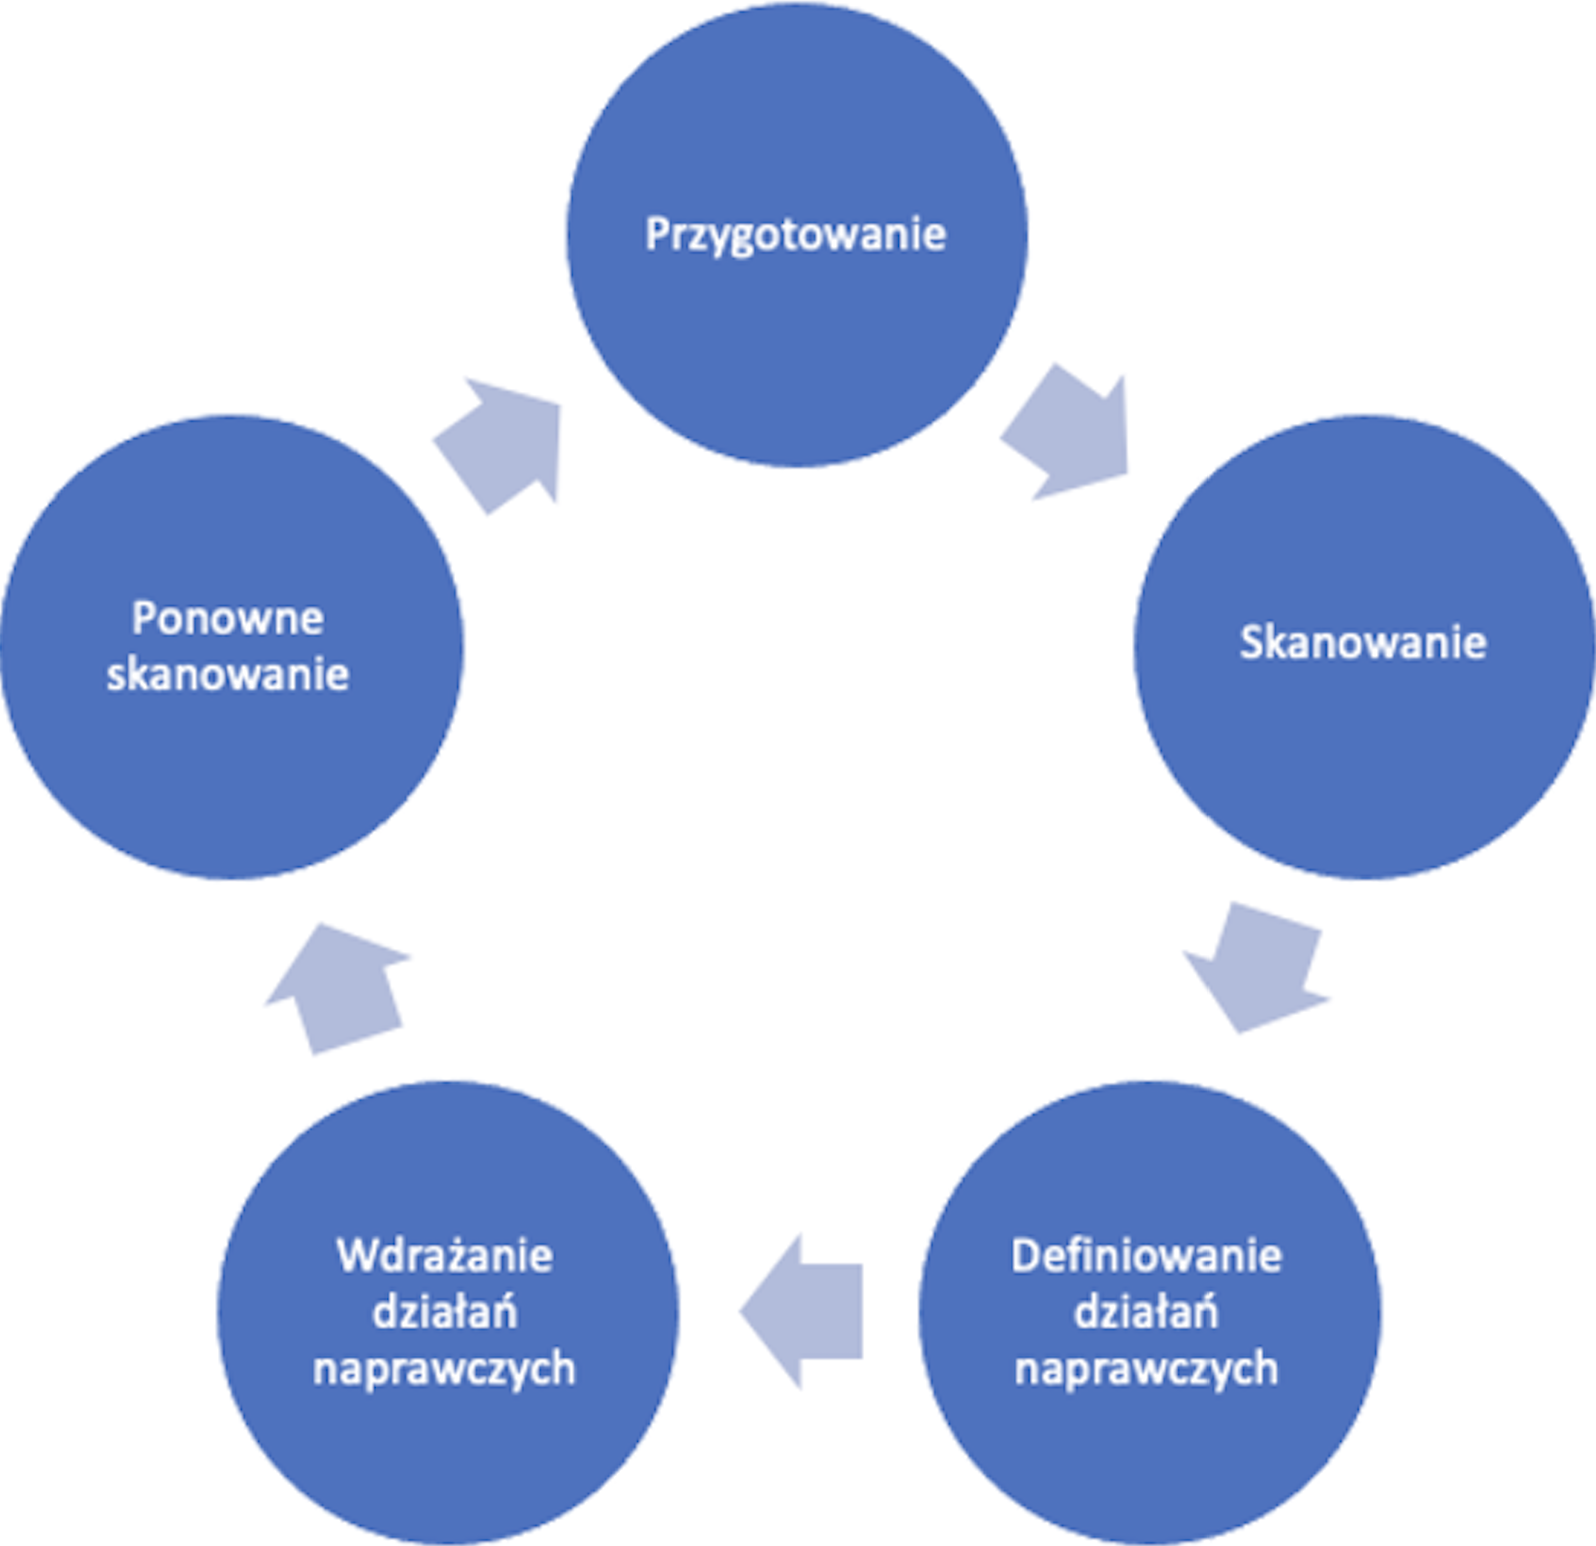
\includegraphics[width=.8\textwidth]{Chapters/Wstep/p-vm/cykl-vm.png}
\caption{Cykl procesu zarządzania podatnościami}
\label{fig:vm-cycle}
\end{figure}

%%%%%%%%%%%%%%%%%%%%%%%%%%%%%%%%%%%%%%%%%%%%%%%%

%%%%%%%%%%%%%%%%%%%%%%%%%%%%%%%%%%%%%%%%%%%%%%%%
\subsection{Przygotowanie}
W pierwszej fazie, przygotowawczej, najważniejsza jest inwentaryzacja zasobów, zapoznanie się ze środowiskiem sieciowym oraz posiadaną infrastrukturą. Po dokonaniu inwentaryzacji oraz zebraniu informacji na temat wykorzystywanego oprogramowania oraz sprzętu dla wszystkich zinwentaryzowanych zasobów nadawane są priorytety, dzięki którym możliwe będzie obliczenie potencjalnego ryzyka oraz podjęcie decyzji, które są kluczowe dla funkcjonowania organizacji.

\bigbreak
Po przeprowadzeniu inwentaryzacji osoba odpowiedzialna za proces, czyli szef bezpieczeństwa, definiuje zakres skanowania, następnie informuje właścicieli oraz administratorów zasobów o planowanym skanowaniu. Każde skanowanie może doprowadzić do obciążenia sieci lub systemów skanowanych, dlatego ważne jest, aby wyznaczyć odpowiednie okno czasowe, dzięki któremu odbywające się skanowanie będzie miało możliwie jak najmniejsze negatywne skutki dla funkcjonowanie skanowanych systemów (Rysunek \ref{fig:vm-prepare}).

\begin{figure}[!ht]
\centering
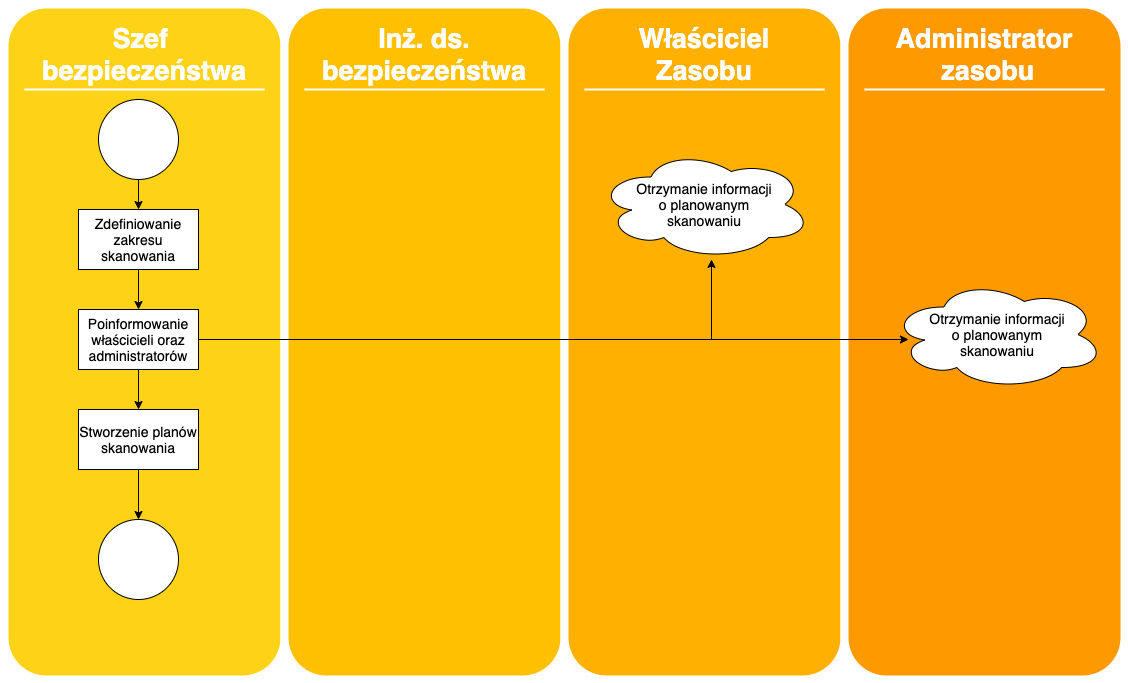
\includegraphics[width=.9\textwidth]{Chapters/Wstep/p-vm/vm-init.png}
\caption{Przepływ informacji w fazie planowania.}
\label{fig:vm-prepare}
\end{figure}
\FloatBarrier

%%%%%%%%%%%%%%%%%%%%%%%%%%%%%%%%%%%%%%%%%%%%%%%%

%%%%%%%%%%%%%%%%%%%%%%%%%%%%%%%%%%%%%%%%%%%%%%%%
\subsection{Skanowanie}
W fazie skanowania zasoby wybrane oraz zinwentaryzowane w fazie przygotowawczej są skanowane przez inż. ds. bezpieczeństwa za pomocą skanera podatności. Duży wpływ na jakość wyników ma zastosowane narzędzie oraz doświadczenie osoby wykonującej skany. W tym czasie również administratorzy zasobów powinni monitorować stabilność swoich systemów. W przypadku wykrycia problemów podczas skanowania administratorzy muszą zgłaszać je do osób wykonujących skanowanie. Wyniki oraz potencjalne problemy dostarczane są do wszystkich osób zaangażowanych w proces zarządzania podatnościami (Rysunek \ref{fig:vm-scanning}).

\begin{figure}[!ht]
\centering
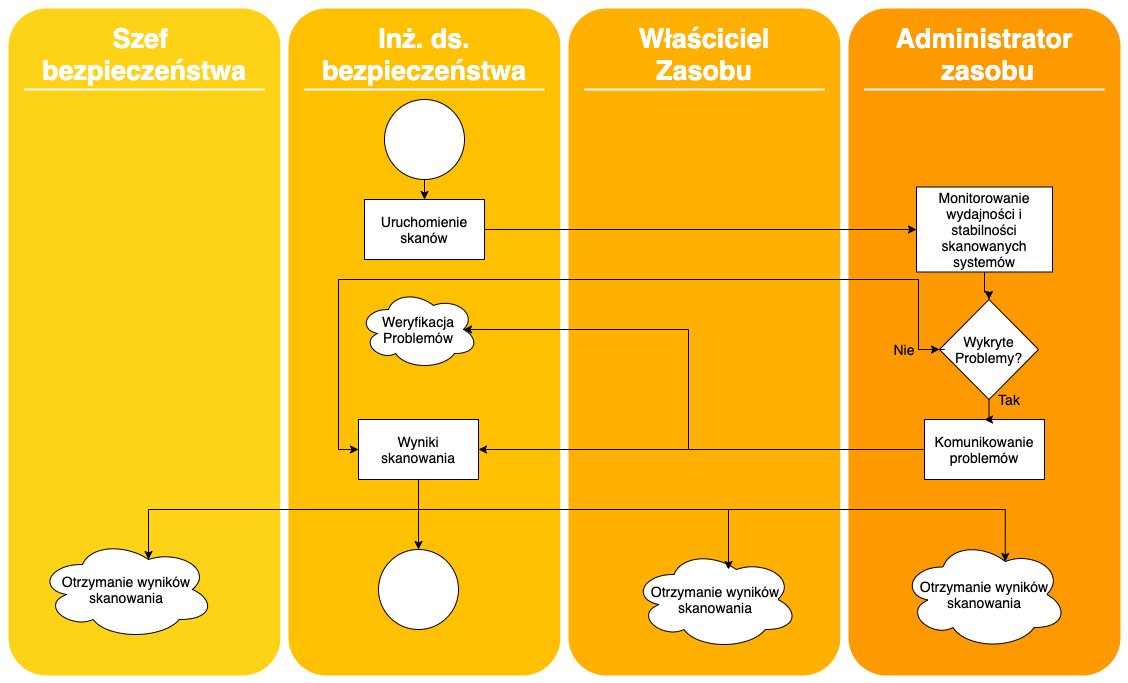
\includegraphics[width=.9\textwidth]{Chapters/Wstep/p-vm/scaninng.png}
\caption{Przepływ informacji w fazie skanowania.}
\label{fig:vm-scanning}
\end{figure}
\FloatBarrier
%%%%%%%%%%%%%%%%%%%%%%%%%%%%%%%%%%%%%%%%%%%%%%%%

%%%%%%%%%%%%%%%%%%%%%%%%%%%%%%%%%%%%%%%%%%%%%%%%
\subsection{Definiowanie działań naprawczych}
W fazie definiowania działań naprawczych zarówno inż. ds. bezpieczeństwa, jak i administrator zasobu powinni przeanalizować wynik skanowania podatności. Po przeprowadzeniu analiz przekazują wnioski i rekomendacje właścicielowi zasobu. Po otrzymaniu wszystkich informacji właściciel zasobu decyduje, czy ryzyko związanie z wykorzystaniem wykrytych podatności jest akceptowalne. Jeśli nie, powinien zdefiniować działania naprawcze. Jeżeli jednak zaakceptuje ryzyko, musi przekazać te informacje do szefa działu bezpieczeństwa w celu rozpoczęcia formalnego procesu akceptacji ryzyka. Nawet bez decyzji o podjęciu działań naprawczych należy zachować odpowiednią dokumentację na wypadek wzrostu ryzyka w przyszłości (Rysunek \ref{fig:vm-fixing}).

\begin{figure}[!ht]
\centering
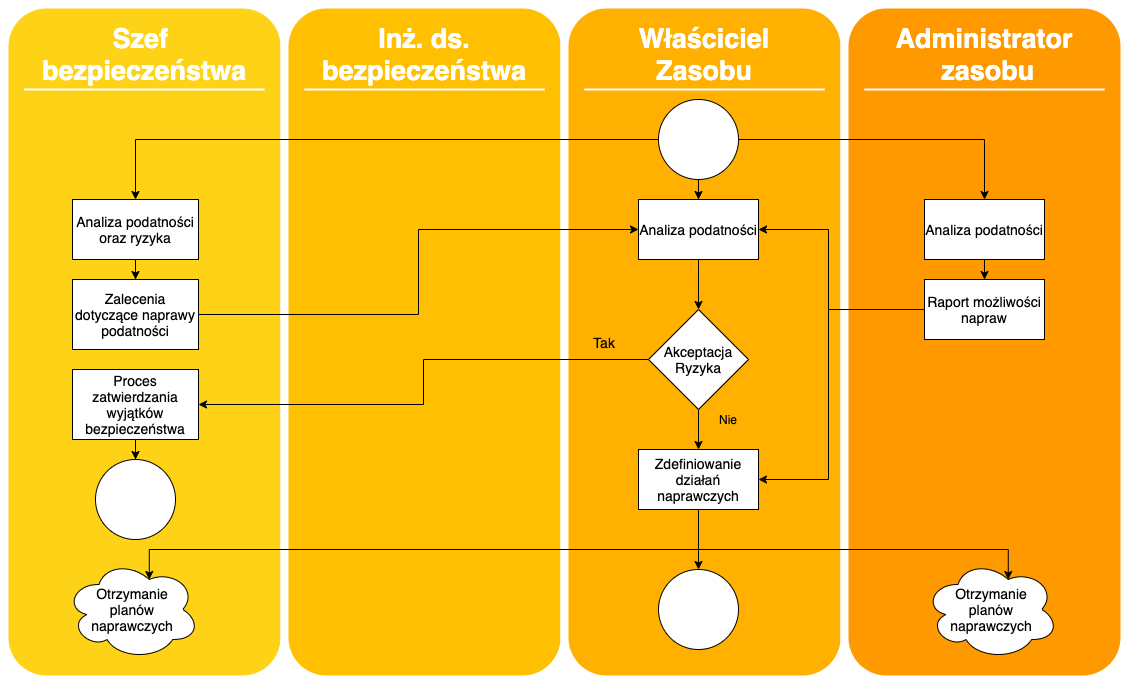
\includegraphics[width=.9\textwidth]{Chapters/Wstep/p-vm/vm-fixing.png}
\caption{Przepływ informacji w fazie definiowania działań naprawczych.}
\label{fig:vm-fixing}
\end{figure}
%%%%%%%%%%%%%%%%%%%%%%%%%%%%%%%%%%%%%%%%%%%%%%%%

%%%%%%%%%%%%%%%%%%%%%%%%%%%%%%%%%%%%%%%%%%%%%%%%
\subsection{Wdrażanie działań naprawczych}
W wielu przypadkach działania łagodzące są łatwiejsze do wdrożenia niż działania naprawcze, jednocześnie zapewniają już wystarczającą ochronę. Poprzez działania łagodzące rozumiemy wykorzystanie firewalli, systemów wykrywania włamań (ang. Intrusion Detection System, w skrócie IPS) lub zapory aplikacji internetowej (ang. Web Application Firewall, w skrócie WAF) – w zależności od dostępnego budżetu oraz zapotrzebowania. Metody łagodzące zamiast naprawy stosowane są w sytuacjach, w których naprawa jest zbyt kosztowna lub zachodzi wysokie ryzyko, że naprawa danej podatności może uszkodzić działanie systemów, przykładowo wgranie nowej wersji oprogramowania spowoduje destabilizację serwera – warto posiadać linię testową, aby przed udostępnieniem poprawki w środowisku produkcyjnym zbadać jak będzie się zachowywał zaktualizowany system. Po wykonaniu wszystkich działań naprawczych administrator powinien poinformować szefa bezpieczeństwa w celu umożliwienia rozpoczęcia kolejnej fazy procesu (Rysunek \ref{fig:flow-fixing}).

\begin{figure}[!ht]
\centering
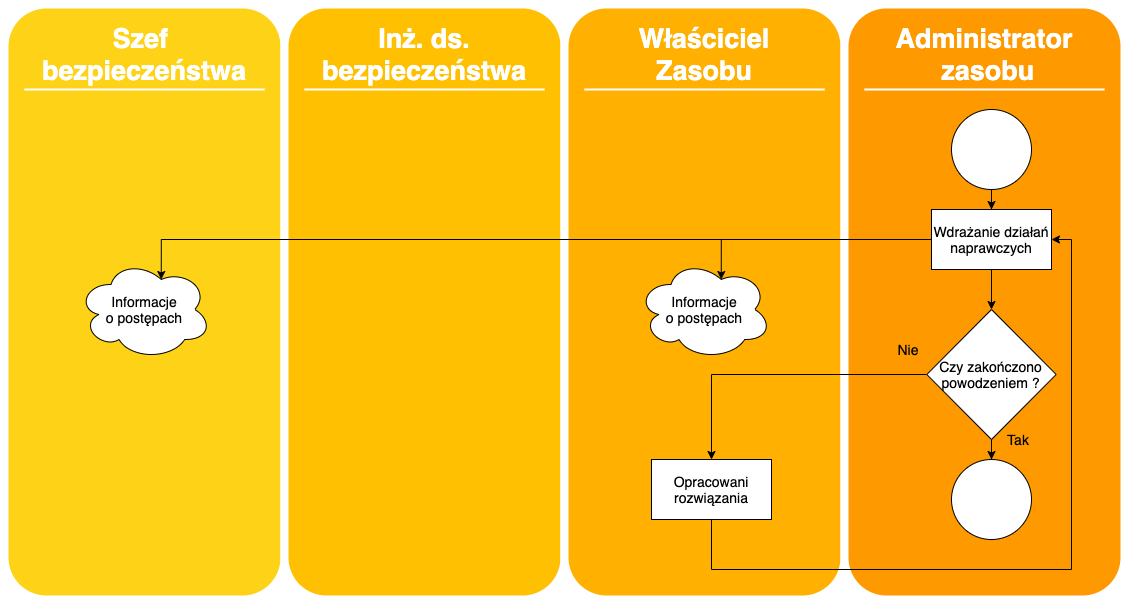
\includegraphics[width=.9\textwidth]{Chapters/Wstep/p-vm/flow-fixing.png}
\caption{Przepływ informacji w fazie wdrażania działań naprawczych.}
\label{fig:flow-fixing}
\end{figure}

%%%%%%%%%%%%%%%%%%%%%%%%%%%%%%%%%%%%%%%%%%%%%%%%

%%%%%%%%%%%%%%%%%%%%%%%%%%%%%%%%%%%%%%%%%%%%%%%%
\subsection{Ponowne skanowanie}
Ostatnia faza polega na uruchomieniu ponownego skanowania przez inżyniera ds. bezpieczeństwa, przeanalizowaniu uzyskanych wyników, a następnie poinformowaniu właściciela zasobu i szefa bezpieczeństwa. Szef bezpieczeństwa ocenia, czy działania naprawcze zakończyły się powodzeniem. W zależności od przyjętej koncepcji fazę tę można potraktować jako rozpoczęcie nowego cyklu życia procesu zarządzania podatnościami (Rysunek \ref{fig:rescan-flow}).
\begin{figure}[!ht]
\centering
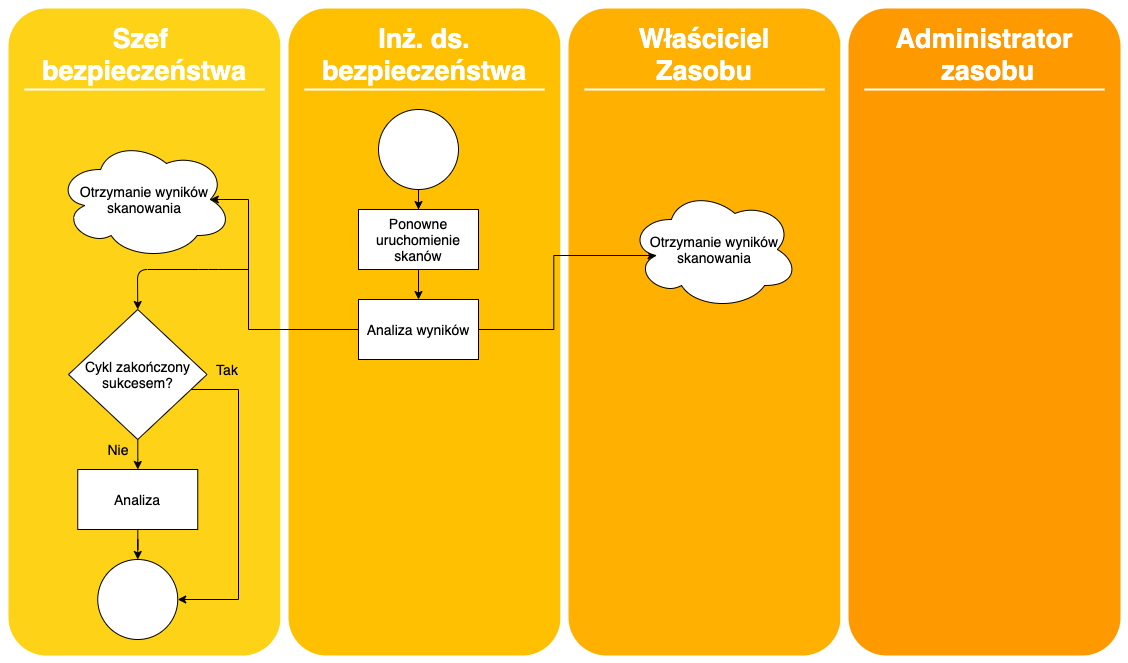
\includegraphics[width=.9\textwidth]{Chapters/Wstep/p-vm/rescan-flow.png}
\caption{Przepływ informacji w fazie ponownego skanowania.}
\label{fig:rescan-flow}
\end{figure}

%%%%%%%%%%%%%%%%%%%%%%%%%%%%%%%%%%%%%%%%%%%%%%%%

%%%%%%%%%%%%%%%%%%%%%%%%%%%%%%%%%%%%%%%%%%%%%%%%
\subsection{Podsumowanie}
Wdrażając proces zarządzania podatnościami, opisany w niniejszym rozdziale, dla każdej organizacji należy rozpocząć od fazy przygotowawczej, która jest najważniejsza. To właśnie w niej zostanie dokonana inwentaryzacja zasobów. Nie jest możliwe wdrożenie procesu, który ma poprawiać bezpieczeństwo organizacji oraz chronić przed zagrożeniami bez wiedzy, co powinno być chronione i na jakim poziomie. Kolejnym krokiem, który musi zostać wykonany, to wyszczególnienie zakresu odpowiedzialności dla wszystkich osób biorących udział w procesie. Ilość osób zaangażowanych w proces zarządzania podatnościami zależy od rozmiaru oraz kontekstu organizacji. Dla małej organizacji zakresy obowiązków zostaną zwiększone, przykładowo właściciel organizacji będzie pełnić funkcje szefa bezpieczeństwa oraz właściciela zasobu, natomiast pracownik będzie inż. ds. bezpieczeństwa oraz administratorem zasobu. Niemniej jednak proces zarządzania podatnościami będzie wyglądał tak samo. Nigdy nie powinno doprowadzać się do tego, aby jedna osoba była odpowiedzialna za wszystkie cztery zakresy odpowiedzialności, ponieważ nigdy nie będzie ona dość obiektywna w podejmowaniu decyzji dotyczącej ryzyka lub naprawy podatności. W dużej organizacji, w której dostępna jest większa liczba pracowników, zwiększy się ilość osób biorących udział w procesie, dzięki czemu zakres odpowiedzialności poszczególnych osób jest ściśle określony.

\bigbreak
W zależności od narzędzi wykorzystywanych oraz przyjętych ram czasowych dotyczących obsługi otrzymanego zgłoszenia w organizacji (ang. Service Level Agreement, w skrócie SLA) finalny czas naprawy podatności będzie się znacząco różnił. Zysk z wykorzystania proponowanego modelu zarządzania podatnościami w każdym przypadku będzie znaczący, a szacunkowa liczba roboczogodzin przedstawiona w rozdziale \ref{sec:modele-ewaluacji-efektywnosci} dla modelu zarządzania podatnościami pozwala na przyjęcie założeń dotyczących planowania czasochłonności oraz liczby zadań potrzebnych do wykonania zgodnie z nowoczesnym modelem pracy, jakim jest Agile \cite{alqudah2016review}. Rolą osób zarządzających zespołami jest zatrudnienie odpowiedniej liczby osób, tak aby pojedynczy pracownik nie stał się tak zwanym wąskim gardłem dla całego procesu zarządzania podatnościami. Na przykład zatrudnienie trzech pracowników może pozwolić na skrócenie liczby wymaganych roboczogodzin trzykrotnie. 

%%%%%%%%%%%%%%%%%%%%%%%%%%%%%%%%%%%%%%%%%%%%%%%%

%%%%%%%%%%%%%%%%%%%%%%%%%%%%%%%%%%%%%%%%%%%%%%%%
\section{Modele zarządzania podatnościami}
\label{sec:modele-zarzadzaia-podatnosciami}
Autorzy w pracach \cite{fruhwirth2009improving, ali2011software} podkreślą fakt, że w celu prawidłowego nadania priorytetu podatności organizacje powinny w ustandaryzowany sposób rozważyć wagę aktywów i ocenę podatności. Problem priorytetyzacji podatności jest od dawna omawiany w dostępnej literaturze \cite{chen2007stakeholder, eschelbeck2005laws, lai2007using, rieke2006modelling}. Większość organizacji o ugruntowanej pozycji, które poważnie traktują cyberbezpieczeństwo, ma wdrożony w mniejszym lub większym stopniu proces zarządzania podatnościami \cite{Gartner-2020, chen2007stakeholder, fruhwirth2009improving}. Jednak, jak zauważono w \cite{Gartner-2020, chen2007stakeholder, eschelbeck2005laws, lai2007using, rieke2006modelling}, każda organizacja podchodzi do problemu inaczej. Rozwiązania wymienione w raporcie \cite{Gartner-vm}, F-Secure \cite{fsecure2021}, Qualys \cite{qualys2021}, Rapid7 \cite{rapid72021} czy Tenable \cite{tenablevm2021} z jednej strony pomagają organizacjom przezwyciężyć problem zarządzania podatnościami, ale z drugiej mają dwie wady. Mianowicie są bardzo drogie i nie informują użytkowników o szczegółach procedury priorytetyzacji podatności. Na przykład Qualys używa 7-punktowej skali \cite{qualys2021}, Rapid7 przeprowadza priorytetyzację w zakresie od 1 do 1000 \cite{rapid72021}, natomiast Tenable nazwał swoją metodę priorytetyzacji VPR, dla której podane poziomy mieszczą się w zakresie od 1 do 10 \cite{tenablevm2021}.

\bigbreak
Oprócz rozwiązań komercyjnych w literaturze można znaleźć inne rozwiązania, takie jak: PatchRank \cite{yadav2019patchrank}, SecureRank \cite{miura2007securerank}, Vulcon \cite{farris2018vulcon}, CMS \cite{weintraub2016security}, czy VEST \cite{chen2019vest}. Rozwiązanie PatchRank skupia się wyłącznie na priorytetyzacji aktualizacji dla systemów SCADA \cite{yadav2019patchrank}. SecureRank wykorzystuje topologię sieci i potencjalną interakcję między serwerami do obliczenia ryzyka \cite{miura2007securerank}. Strategia oprogramowania Vulcon opiera się na dwóch elementarnych wskaźnikach: czasie pojawienia się podatności i całkowitym czasie ekspozycji na podatność \cite{farris2018vulcon} w cyklach miesięcznych. CMS skupia się na wykrywaniu podatności na podstawie korelacji bazy zasobów z bazą NVD, w związku z czym istnieje duże prawdopodobieństwo zgłaszania przez narzędzie podatności, które rzeczywiście nie istnieją lub pomijanie tych, które naprawdę znajdują się w środowisku \cite{weintraub2016security}. VEST natomiast skupia się na przewidywaniu jak szybko podatność może zostać wykorzystana przez atakującego \cite{chen2019vest}. Inne rozwiązania, np. \cite{yadav2019patchrank, miura2007securerank, farris2018vulcon, chen2019vest} nie uwzględniają wag zasobów i nie są dostosowane do rosnącej ilości danych w środowisku chmury obliczeniowej, przez co nie mogą być stosowane w każdej infrastrukturze sieciowej. Dodatkowo żadne z przedstawionych rozwiązań nie oferuje jednocześnie priorytetów dla CVSS 2.0 i CVSS 3.x. Wynika to z faktu, że nie wszystkie podatności zostały przekonwertowane z CVSS 2.0 do CVSS 3.x, mimo że CVSS 3.x lepiej ocenia istotę podatności i skuteczniej szacuje zagrożenia \cite{fall2019common, Nowak-cldd-2021, Nowa2109Conversion}.

\begin{figure}[!ht]
\centering
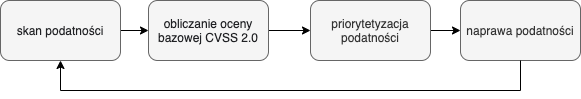
\includegraphics[width=.9\textwidth]{Chapters/Wstep/vm-models/vm-model-cvss2.png}
\caption{Model przepływu informacji w procesie zarządzania podatnościami z wykorzystaniem oceny bazowej CVSS 2.0.}
\label{fig:chapter1:vm-model-cvss2}
\end{figure}

\bigbreak
Wszystkie przedstawione wcześniej rozwiązania nie obejmują priorytetyzacji wykrytych podatności według oceny środowiskowej, przez co proces zarządzania podatnościami odbywa się z wykorzystaniem ocen bazowych. Rysunki \ref{fig:chapter1:vm-model-cvss2} i \ref{fig:chapter1:vm-model-cvss3} przestawiają modele procesu zarządzania podatnościami z wykorzystaniem ocen bazowych CVSS, w którym to wyniki otrzymane bezpośrednio ze skanera są prioretyzowane, a następnie przekazywane do administratorów zasobów w celu wykonania prac naprawczych. Na dodatkową uwagę zasługuje również fakt, że organizacje wspierają się metrykami zaproponowanymi przez Center for Internet Security (CIS), które powstały w 2010 roku \cite{CIS-2010, Walk2109-Automatic} w celu mierzenia stanu bezpieczeństwa infrastruktury teleinformatycznej. Organizacje, aby spełnić wymagania stawiane przez metryki CIS, najczęściej wybierają standard oparty na ocenie bazowej CVSS 2.0 (Rysunek \ref{fig:chapter1:vm-model-cvss2}), pomijając model \ref{fig:chapter1:vm-model-cvss3} z uwagi na wcześniej wspomnianą wadę CVSS 3.x dotyczącą braku oceny bazowej dla wszystkich podatności.


\begin{figure}[!ht]
\centering
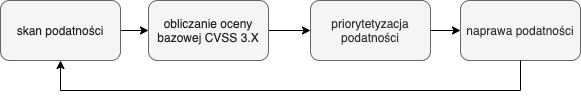
\includegraphics[width=.9\textwidth]{Chapters/Wstep/vm-models/vm-model-cvss3.png}
\caption{Model przepływu informacji w procesie zarządzania podatnościami z wykorzystaniem oceny bazowej CVSS 3.x.}
\label{fig:chapter1:vm-model-cvss3}
\end{figure}

\bigbreak
Autorzy takich prac jak \cite{fruhwirth2009improving, wang2015vulnerability, gallon2010impact} zauważyli, że wskazane modele wykorzystujące ocenę bazową (Rysunek \ref{fig:chapter1:vm-model-cvss2}, \ref{fig:chapter1:vm-model-cvss3}) są niewystarczające i oprócz nich należy brać jeszcze pod uwagę kontekst organizacji w celu dokładniejszego oszacowania poziomu bezpieczeństwa. Dlatego w niniejszej pracy zaproponowano dwa modele procesu zarządzania podatnościami wykorzystujące ocenę środowiskową CVSS. Rysunek \ref{fig:chapter1:vm-model-cvss2e} i \ref{fig:chapter1:vm-model-cvss3e} przedstawiają modele, które dodatkowo pobierają informacje o wagach zasobów z przygotowanej wcześniej bazy zasobów IT, dzięki czemu wykonują reprioretyzacje podatności uwzględniając ocenę środowiskową, która pozwala na lepsze dopasowanie oceny podatności do kontekstu organizacji. Tym samym pozwalają na identyfikacje wszystkich istotnych podatności bezpieczeństwa infrastruktury teleinformatycznej. Model pierwszy (Rysunek \ref{fig:chapter1:vm-model-cvss3e}), wykorzystujący ocenę środowiskową CVSS 3.x, posiada takie same wady jak wcześniej wspominany model wykorzystujący ocenę bazową CVSS 3.x (Rysunek \ref{fig:chapter1:vm-model-cvss3}) dotyczący braku oceny dla wszystkich podatności, dlatego również nie jest w stanie spełnić wymagań stawianych przez proponowane metryki CIS. Natomiast dzięki zastosowaniu metod konwersji oceny bazowej CVSS 2.0 do CVSS 3.x, przedstawionych w \cite{Nowa2109Conversion, Nowak-cldd-2021} możliwe jest jego w pełni zastosowanie. Model drugi (Rysunek \ref{fig:chapter1:vm-model-cvss2e}) z wykorzystaniem oceny środowiskowej CVSS 2.0 nie może być rozpatrywany jako samodzielny, ponieważ wpływ parametru $TD$, służący do ustalania liczby systemów wrażliwych na daną podatność, będzie znacząco zaniżał oceny wszystkich wykrytych podatności, w związku z czym stworzy on złudne wrażenie bezpieczeństwa monitorowanej infrastruktury teleinformatycznej, czyniąc ją bardziej podatną na ataki hakerskie. W rozdziale czwartym oraz piątym przedstawiony zostanie wpływ priorytetyzacji podatności za pomocą przedstawionych modeli na proces zarządzania podatnościami w celu weryfikacji tezy przedstawionej w rozdziale \ref{sec:zakres-i-teza-pracy}.

\begin{figure}[!ht]
\centering
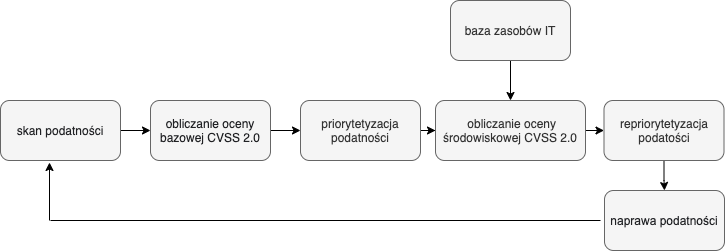
\includegraphics[width=.9\textwidth]{Chapters/Wstep/vm-models/vm-model-cvss-e-2.png}
\caption{Model przepływu informacji w procesie zarządzania podatnościami z wykorzystaniem oceny środowiskowej CVSS 2.0.}
\label{fig:chapter1:vm-model-cvss2e}
\end{figure}

\begin{figure}[!ht]
\centering
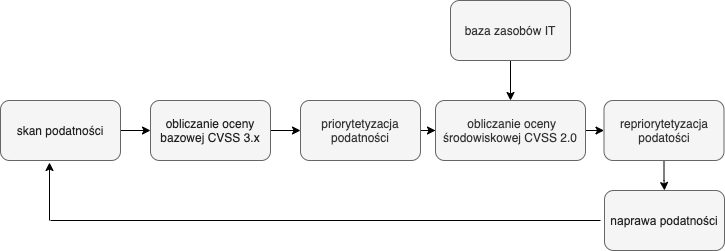
\includegraphics[width=.9\textwidth]{Chapters/Wstep/vm-models/vm-model-cvss-e-3.png}
\caption{Model przepływu informacji w procesie zarządzania podatnościami z wykorzystaniem oceny środowiskowej CVSS 3.x.}
\label{fig:chapter1:vm-model-cvss3e}
\end{figure}

\bigbreak
Kolejną ważną cechą opracowaną w niniejszej pracy jest również rozwiązanie problemu skalowalności. Pozwala to na łatwe dopasowanie narzędzia do rosnącej ilości napływających danych. Zgodnie z wynikami i dyskusjami przedstawionymi w dostępnej literaturze istotnym elementem zarządzania dużymi zbiorami danych jest ich cykl życia. W \cite{el2017data} autorzy przeanalizowali kilkanaście różnych cykli życia danych i ich faz, dążąc do znalezienia tych, które „czynią dane inteligentnymi, a tym samym ułatwiają zarządzanie nimi w kontekście Big Data”. „Inteligentny” oznacza wspomnianą wcześniej wiedzę uzyskaną z dużego i początkowo niestrukturyzowanego zbioru danych. Według \cite{lenk2015towards} „fazy składające się na cykl życia danych w kontekście Big Data są bardzo złożone. Każda faza jest uważana za jeden lub więcej złożonych, operacyjnych i niezależnych procesów, ale procesy te są ze sobą powiązane i sprawiają, że zarządzanie danymi jest bardziej elastyczne i inteligentne”. Zatem przedstawienie cyklu życia danych nie jest zadaniem trywialnym. W porównaniu z \cite{yadav2019patchrank, miura2007securerank, farris2018vulcon, chen2019vest} opracowane na potrzeby pracy doktorskiej oprogramowanie wykorzystuje informacje zebrane z bazy danych zasobów. W przeciwieństwie do \cite{fsecure2021, qualys2021, rapid72021, tenablevm2021} procedura ustalania priorytetów została szczegółowo opisana i dlatego może być analizowana przy użyciu standardu FIRST \cite{cvs2005specification, cvs2019specification}. Opracowane oprogramowanie jako produkt open source \cite{vmcgithub} charakteryzuje się przejrzystością stosowanych metod i technik.

\FloatBarrier
%%%%%%%%%%%%%%%%%%%%%%%%%%%%%%%%%%%%%%%%%%%%%%%%

%%%%%%%%%%%%%%%%%%%%%%%%%%%%%%%%%%%%%%%%%%%%%%%%
\section{Modele ewaluacji efektywności zarządzania podatnościami}
\label{sec:modele-ewaluacji-efektywnosci}
W celu ewaluacji efektywności modeli zarządzania podatnościami (Rysunek \ref{fig:chapter1:vm-model-cvss2}, \ref{fig:chapter1:vm-model-cvss3}, \ref{fig:chapter1:vm-model-cvss2e}, \ref{fig:chapter1:vm-model-cvss3e}) wykorzystano metrykę czasową zaprezentowaną w pracy \cite{farris2018vulcon}. Metryka mierzy szacunkową liczbę roboczogodzin wymaganych do poprawienia bezpieczeństwa infrastruktury. Autorzy pracy \cite{farris2018vulcon} przeprowadzili wywiad z inżynierami odpowiedzialnymi za naprawę podatności oraz podzielili je na trzy możliwe kategorie:
\begin{itemize}
    \item od 1 do 3 godzin (słabe metody szyfrowania, domyślne hasło lub poprawa konfiguracji),
    \item od 3 do 6 godzin (naprawa poprzez aktualizacje wersji oprogramowania),
    \item od 6 do 9 godzin (naprawa poprzez aktualizacje systemu operacyjnego).
\end{itemize}

Korzystając ze wspomnianych zakresów roboczogodzin, czas naprawy podatności ($T_{FIX}$) został podzielony na trzy podkategorie. Biorąc pod uwagę liczbę godzin potrzebnych do naprawy, $T_{FIX_{MAX}}$ reprezentuje maksymalną liczbę roboczogodzin wymaganą do naprawy jednej podatności (9 godzin), $T_{FIX_{AVERGE}}$ reprezentuje średnią liczbę roboczogodzin wymaganą do naprawienia jednej podatności (4.5 godziny) oraz $T_{FIX_{MIN}}$ reprezentuje minimalną liczbę roboczogodzin, która jest równa 1 godzinie. Następnie opracowano równania pozwalające oszacować liczbę roboczogodzin wymaganą do usunięcia istotnych podatności bezpieczeństwa infrastruktury teleinformatycznej. 

\bigbreak
Przy założeniu, że wszystkie podatności o klasyfikacji krytycznej ($X_C$), wysokiej ($X_H$) oraz średniej ($X_M$) muszą zostać naprawione przez administratorów, zakres wymaganej liczby roboczogodzin potrzebnych do usunięcia istotnych podatności bezpieczeństwa za pomocą proponowanych modeli zarządzania podatnościami można wyrazić za pomocą sumy iloczynów liczby podatności, które mają zostać naprawione oraz szacowanej liczby roboczogodzin, uwzględniającej czas trwania naprawy podatności. Dodatkowo w równaniu należy uwzględnić czas trwania skanowania ($T_S$). Dla modelu opartego o ocenę bazową CVSS 2.0 (Rysunek \ref{fig:chapter1:vm-model-cvss2}) równanie będzie miało następującą postać:
\begin{equation}
\label{eq:cvss2}
T_{Base2} = T_S + (T_{FIX} \cdot X_{H_\text{CVSS 2.0 Base}}) + (T_{FIX} \cdot X_{M_\text{CVSS 2.0 Base}})
\end{equation}
Gdzie $T_{FIX}$ to liczba roboczogodzin wymaganych do naprawy jednej podatności, $X_{H_\text{CVSS 2.0 Base}}$, $X_{M_\text{CVSS 2.0 Base}}$ to liczba podatności o odpowiednio wysokim i średnim poziomie krytyczności, zgodnie z oceną bazową CVSS 2.0.

\bigbreak
\begin{multline}
\label{eq:cvss3}
T_{Base3} = T_S + (T_{FIX} \cdot X_{C_\text{CVSS 3.x Base}}) + (T_{FIX} \cdot X_{H_\text{CVSS 3.x Base}}) + (T_{FIX} \cdot X_{M_\text{CVSS 3.x Base}}) 
\end{multline}
Gdzie $X_{C_\text{CVSS 3.x Base}}$ $X_{H_\text{CVSS 3.x Base}}$, $X_{M_\text{CVSS 3.x Base}}$ to liczba podatności o odpowiednio krytycznym, wysokim i średnim poziomie krytyczności zgodnie z oceną bazową CVSS 3.x.

\bigbreak
Ponieważ ocena bazowa CVSS jest oceną subiektywną, osoby zaangażowane w proces nie mają pewności, czy w kategorii o krytyczności niskiej ($X_L$) nie znajdują się podatności, które z punktu widzenia organizacji są istotne, czyli podatności o niedoszacowanej ocenie. Z tego względu administratorzy powinni naprawić wszystkie podatności, aby wyeliminować zaistniałe ryzyko nienaprawienia podatności z niedoszacowaną oceną \cite{gallon2010impact, li2015study}. Proponowane równanie dla modelu wykorzystującego ocenę bazową CVSS 2.0 (Rysunek \ref{fig:chapter1:vm-model-cvss2}) minimalizujące ryzyko nienaprawienia podatności niedoszacowanej będzie miało następującą postać:
\begin{equation}
\label{eq:cvss2prim}
T_{Base2'} = T_S + (T_{FIX} \cdot X_{H_\text{CVSS 2.0 Base}}) + (T_{FIX} \cdot X_{M_\text{CVSS 2.0 Base}}) + (T_{FIX} \cdot X_{L_\text{CVSS 2.0 Base}})
\end{equation}
Gdzie $T_{FIX}$ to liczba godzin pracy wymaganych do naprawy jednej podatności, $X_{H_\text{CVSS 2.0 Base}}$, $X_{M_\text{CVSS 2.0 Base}}$, $X_{ L_\text{CVSS 2.0 Base}}$ to liczba podatności o odpowiednio wysokim, średnim i niskim poziomie krytyczności, zgodnie z otrzymaną oceną bazową CVSS 2.0.

\bigbreak
Dla modelu zarządzania podatnościami opartego o ocenę bazową CVSS 3.x (Rysunek \ref{fig:chapter1:vm-model-cvss3}):
\begin{multline}
\label{eq:cvss3prim}
T_{Base3'} = T_S + (T_{FIX} \cdot X_{C_\text{CVSS 3.x Base}}) + (T_{FIX} \cdot X_{H_\text{CVSS 3.x Base}}) + (T_{FIX} \cdot X_{M_\text{CVSS 3.x Base}}) + \\
+ (T_{FIX} \cdot X_{L_\text{CVSS 3.x Base}})
\end{multline}
Gdzie $X_{C_\text{CVSS 3.x Base}}$ $X_{H_\text{CVSS 3.x Base}}$, $X_{M_\text{CVSS 3.x Base}}$, $X_ {L_\text{CVS 3.x Base}}$ to liczbą podatności o odpowiednio krytycznym, wysokim, średnim i niskim poziomie krytyczności zgodnie z otrzymaną oceną bazową CVSS 3.x.

\bigbreak
W przypadku modeli wykorzystujących ocenę środowiskową dodatkowo należy uwzględnić w równaniu czas ponownej priorytetyzacji za pomocą wytworzonego oprogramowania ($T_{VMC}$) oraz usunąć część równania odpowiedzialną za liczbę roboczogodzin potrzebnych do naprawy podatności niskich, ponieważ zakładamy, że ocena środowiskowa poprawnie wykonała prioretetyzacje z uwzględnieniem wymagań organizacji, w związku z czym wszystkie podatności zostały przypisane do odpowiadającej im kategorii, tym samym minimalizując ryzyko nienaprawienia niedoszacowanej oceny podatności. Dokładna możliwość zmiany oceny oraz kategorii podatności zostały szerzej omówione w rozdziale piątym. 

\bigbreak
Dla modelu środowiskowego CVSS 2.0 (Rysunek \ref{fig:chapter1:vm-model-cvss2e}) równanie przyjmie następującą postać:
\begin{equation}
\label{eq:cvss2e}
T_{Env2} = T_S + T_{VMC} + (T_{FIX} \cdot X_{H_\text{CVSS 2.0 Environmental}}) + (T_{FIX} \cdot X_{M_\text{CVSS 2.0 Environmental}})
\end{equation}
Gdzie $T_{VMC}$ jest czasem trwania ponownej priorytetyzacji wykonanej za pomocą opracowanego oprogramowania, $X_{H_\text{CVSS Environmental 2.0}}$ i $X_{M_\text{CVSS Environmental 2.0}}$ są odpowiednio liczbą podatności o wysokim i średnim poziomie krytyczności według oceny środowiskowej CVSS 2.0.

\bigbreak
Analogicznie dla przypadku modelu środowiskowego CVSS 3.x (Rysunek \ref{fig:chapter1:vm-model-cvss2e}):
\begin{multline}
\label{eq:cvss3e}
T_{Env3} = T_S + T_{VMC} + (T_{FIX} \cdot X_{C_\text{CVSS 3.x Environmental}}) + (T_{FIX} \cdot X_{H_\text{CVSS 3.x Environmental}}) + \\
+ (T_{FIX} \cdot X_{M_\text{CVSS 3.x Environmental}})
\end{multline}
Gdzie $X_{C_\text{CVSS 3.x Environmental}}$, $X_{H_\text{CVSS 3.x Environmental}}$ i $X_{M_\text{CVSS 3.x Environmental}}$ to odpowiednio liczba podatności o krytycznej, wysokiej i średniej krytyczności zgodnie z oceną środowiskową CVSS 3.x.

\bigbreak
Porównanie łącznej liczby roboczogodzin wymaganych do usunięcia podatności o kategorii krytycznej, wysokiej oraz średniej dla zaproponowanych modeli zarządzania podatnościami pozwoli określić bardziej wydajne rozwiązanie, a tym samym potwierdzić tezę przedstawioną w podrozdziale \ref{sec:zakres-i-teza-pracy}. Różnica liczby roboczogodzin między badanymi modelami zarządzania podatnościami określa potencjalne oszczędności, które można osiągnąć poprzez zmiany w mechanizmach priorytetyzacji podatności.

%%%%%%%%%%%%%%%%%%%%%%%%%%%%%%%%%%%%%%%%%%%%%%%%

%%%%%%%%%%%%%%%%%%%%%%%%%%%%%%%%%%%%%%%%%%%%%%%%
\section{Zakres i teza pracy}
\label{sec:zakres-i-teza-pracy}
Obecnie stosowane systemy priorytetyzacji podatności działają przy wykorzystaniu standardu CVSS 2.0 oceny krytyczności podatności. Ponadto skanery podatności obliczają jedynie ocenę bazową (ang. Base Score), a zatem nie uwzględniają wielu istotnych danych, które są potencjalnie dostępne dla operatora sieci teleinformatycznej. Takie podejście do zagadnienia priorytetyzacji podatności może skutkować błędnym zaszeregowaniem danej podatności. To z kolei może być przyczyną zwiększenia czasu pozostawania w systemie wielu podatności krytycznych, a tym samym zwiększa ryzyko naruszenia bezpieczeństwa zasobów.

\bigbreak
Teza pracy jest zatem następująca:

\bigbreak
\emph{Przy łącznym wykorzystaniu danych, które zawierają istotne informacje na temat infrastruktury sieci teleinformatycznej oraz danych pochodzących ze skanerów podatności możliwe jest w oparciu o otwarty standard CVSS (ang. Common Vulnerability Scoring System) stworzenie algorytmów zarządzania podatnościami o zwiększonej dokładności priorytetyzacji podatności bezpieczeństwa infrastruktury teleinformatycznej w porównaniu z rozwiązaniami opartymi jedynie na ocenie bazowej CVSS 2.0. Dzięki temu możliwe jest zmniejszenie liczby roboczogodzin potrzebnych do usunięcia istotnych podatności, a zatem także zmniejszenie czasu pozostawania tychże podatności w systemie.}

\bigbreak
Opracowany pakiet oprogramowania jest w zasadzie praktyczną realizacją Centrum Zarządzania Podatnościami (ang. Vulnerability Management Center, w skrócie VMC)  \cite{vmcgithub}. Zrealizowany w ramach tej pracy VMC pobiera informacje o zasobach IT z bazy inwentaryzacyjnej organizacji \cite{ralph} oraz podatności wykryte w monitorowanej infrastrukturze przy pomocy oprogramowania skanującego \cite{beale2004nessus, rahalkar2019openvas}. Następnie wykonuje ponowną priorytetyzację, wykorzystując standard CVSS 2.0 oraz 3.x, a zatem umożliwia realizację wszystkich rozważanych modeli procesu zarządzania podatnościami (Rysunki \ref{fig:chapter1:vm-model-cvss2}, \ref{fig:chapter1:vm-model-cvss3}, \ref{fig:chapter1:vm-model-cvss2e}, \ref{fig:chapter1:vm-model-cvss3e}).  Skuteczność metod priorytetyzacji podatności, które zaproponowano w tej pracy, została zweryfikowana na danych pozyskanych z rzeczywistych środowisk teleinformatycznych przy zastosowaniu metod przedstawionych w rozdziale \ref{sec:modele-ewaluacji-efektywnosci}. 

\bigbreak
Ponadto stworzone oprogramowanie VMC zostało wykorzystane w ramach realizacji projektu badawczego RegSoc \cite{regsoc}. Dokładny opis oprogramowania oraz sposobu implementacji zastosowanych metryk i reguł w projekcie RegSoc znajduje się w załącznikach Z3, Z4 i Z5.

%%%%%%%%%%%%%%%%%%%%%%%%%%%%%%%%%%%%%%%%%%%%%%%%

%%%%%%%%%%%%%%%%%%%%%%%%%%%%%%%%%%%%%%%%%%%%%%%%
\section{Układ pracy}
W rozdziale drugim opisano proponowane rozwiązania oraz architekturę stworzonego oprogramowania  wspomagającego proces zarządzania podatnościami w organizacjach \cite{rochford2008t, Gartner-2020}. Opracowane oprogramowanie korzysta z elementów infrastruktury, takich jak: skaner podatności \cite{beale2004nessus, rahalkar2019openvas}, publicznie dostępne bazy wiedzy o opublikowanych podatnościach \cite{booth2013national, exploitexploits}, systemy inwentaryzacji zasobów IT \cite{baron2010configuration} oraz systemy obsługi zgłoszeń \cite{thehive}. Dzięki normalizacji danych oraz przejrzystości interfejsu w przystępny sposób prezentuje w czasie rzeczywistym informacje dotyczące zagrożeń oraz alarmuje o odstępstwach od normy i anomaliach. Architektura rozwiązania umożliwia uruchomienie go w dowolnym środowisku w zależności od zapotrzebowania. Może to być chmura publiczna, chmura prywatna, serwer fizyczny lub maszyna wirtualna.

\bigbreak
Rozdział trzeci zawiera opis środowisk badawczych, w których przeprowadzono analizę zaproponowanych modeli zarządzania podatnościami. Wszystkie adresy IP wykorzystanych zasobów zostały zanonimizowane, ponieważ otrzymane dane pochodzą z rzeczywistych raportów oraz zawierają informacje poufne, które po ujawnieniu mogą wytworzyć dodatkowe zagrożenie dla organizacji, z których dane zostały pozyskane. Dodatkowo część administratorów dostarczyła informacje dotyczące ustawień środowiskowych z uwzględnieniem wag monitorowanych zasobów, dzięki czemu możliwe było odwzorowanie zachowania oprogramowania w warunkach laboratoryjnych.

\bigbreak
Rozdział czwartym poświęcony jest zbadaniu wpływu poszczególnych parametrów środowiskowych na ocenę bazową.  Uzyskane wyniki pozwoliły na wyciągnięcie wniosków dotyczących wykorzystania zmodyfikowanych równań przedstawionych w podrozdziale \ref{sec:modele-ewaluacji-efektywnosci} dotyczących szacowanej liczby roboczogodzin (Równania \ref{eq:cvss2e}, \ref{eq:cvss3e}).

\bigbreak
W rozdziale piąty omówione są najważniejsze wyniki analizy, które zostały przeprowadzone dla zaproponowanych modeli zarządzania podatnościami oraz opracowanego oprogramowania. Analiza została przeprowadzona na rzeczywistych zbiorach danych. Wykorzystane modele ewaluacji efektywności zarządzania podatnościami przedstawione w podrozdziale \ref{sec:modele-ewaluacji-efektywnosci} pozwoliły na zbadanie zmian zachodzących w priorytetyzacji podatności.

\bigbreak
Podsumowanie zawiera główne wnioski i opis dalszych kierunków badań, bibliografię oraz załączniki. W załącznikach zaś znajduje się dokumentacja dostarczona dla projektu Regionalne Centrum Bezpieczeństwa Cybernetycznego (RegSoc) zrealizowanego przez Wrocławskie Centrum Sieciowo-Super-komputerowe Politechniki Wrocławskiej \cite{regsoc}.

\chapter{Proponowane rozwiązania}
W poprzednim rozdziale opisane zostały zagrożenia związane z publicznie znanymi podatnościami oraz sposób, w jaki radzą sobie organizacje w celu utrzymywania ryzyka na jak najniższym możliwym poziomie. Postawiona została teza pracy oraz zaproponowane modele ewaluacji.

\bigbreak
W niniejszym rozdziale przedstawiono wytworzone oprogramowanie Vulnerability Management Center (VMC), które powstało na potrzeby realizacji pracy doktorskiej w celu potwierdzenia tezy zawartej w rozdziale \ref{sec:zakres-i-teza-pracy}. Oprogramowanie VMC zostało opracowane z wykorzystaniem technologii, takich jak Docker \cite{anderson2015docker} i Kubernetes \cite{chemashkinkubernetes}, z wykorzystaniem algorytmu zaproponowanego w rozdziale \ref{sec:scaling}, dzięki czemu VMC jest dostosowane do rosnącej ilości napływających danych poprzez wykorzystanie mechanizmów skalowania. W dalszej części rozdziału przedstawiony został sposób implementacji parametrów $CDP$, $TD$, wykorzystana metoda konwersji oceny bazowej CVSS 2.0 do CVSS 3.x oraz metoda wykorzystana w analizie liczby oraz zakresu zmian w ocenach podatności.

\bigbreak
Przedstawione technologie oraz mechanizmy zaimplementowane w oprogramowaniu VMC przetestowane zostały w projekcie badawczym RegSoc \cite{regsoc}. Dodatkowo przed wdrożeniem oprogramowania wykonane zostały testy bezpieczeństwa i testy funkcjonalne przez firmę zewnętrzną, potwierdzające poprawność oraz stabilność przedstawionego rozwiązania. VMC od początku projektowane było jako system wspierający bezpieczeństwo monitorowanej infrastruktury teleinformatycznej w związku z czym, rozwijane było zgodnie z metodologią wytwarzania oprogramowania opartego na testach (ang. Test Driven Development, w skrócie TDD) \cite{astels2003test} z wykorzystaniem rekomendacji opisanych w Standardzie Weryfikacji Bezpieczeństwa Aplikacji OWASP (ang. Application Security Verification Standard, w skrócie ASVS) w wersji 4.0.2 poziom 2 \cite{ASVS}.

%%%%%%%%%%%%%%%%%%%%%%%%%%%%%%%%%%%%%%%%%%%%%%%%

%%%%%%%%%%%%%%%%%%%%%%%%%%%%%%%%%%%%%%%%%%%%%%%%
\section{Wprowadzenie do konteneryzacji}
\label{sec:docker}
Docker po raz pierwszy został zaprezentowany w 2013 roku na konferencji Python Developers \cite{bernstein2014containers}. W ciągu kilku tygodni od prezentacji pojawiło się duże zainteresowanie projektem, w związku z czym został on udostępniony na licencji otwartego oprogramowania (ang. open source) w serwisie Github. Docker to narzędzie, którego celem jest uproszczenie dystrybucji aplikacji, którą można wdrażać na dużą skalę w dowolnym środowisku. Docker ma na celu usprawnienie przepływu pracy oraz zwiększenie szybkości reagowania w organizacjach pracujących nad oprogramowaniem w modelu agile \cite{panthofer2019mastering}. Sama konteneryzacja nie jest niczym nowym, jednak przed wprowadzeniem Dockera \cite{anderson2015docker} była jedynie znana osobom, które profesjonalnie zajmowały się oprogramowaniem z wykorzystaniem niskopoziomowych koncepcji oferowanych przez Linux Kernel Containment (LXC). W chwili obecnej trudno jest znaleźć aplikację w której nie wspomina się lub nie wykorzystuje konteneryzacji. Docker przyspiesza cykle rozwoju oprogramowania, zmniejsza koszty infrastruktury, pomaga szybciej wdrażać nowych programistów, a nawet obniża bariery pomiędzy zespołami odpowiedzialnymi za rozwój oraz utrzymanie usług świadczonych przez organizacje. Docker nie zastępuje maszyny wirtualnej, natomiast jest jej dopełnieniem w architekturze chmurowej.

%%%%%%%%%%%%%%%%%%%%%%%%%%%%%%%%%%%%%%%%%%%%%%%%

%%%%%%%%%%%%%%%%%%%%%%%%%%%%%%%%%%%%%%%%%%%%%%%%
\subsection{Korzyści wynikające z zastosowania Dockera}
Niezwykle trudne jest wymienienie wszystkich zalet wykorzystania konteneryzacji. Samo skorzystanie z tej technologii przynosi już wiele korzyści dla samej organizacji, np. poprzez uproszczenie procesów wdrażania oprogramowania (Rysunek \ref{fig:chapter3:proces-without-docker}, \ref{fig:chapter3:proces-with-docker}). Docker ułatwia również podejmowanie decyzji dotyczącej architektury, ponieważ wszystkie aplikacje z punktu widzenia systemu operacyjnego, w którym są uruchomione, wyglądają dokładnie tak samo. Dodatkowo w literaturze można znaleźć korzyści, takie jak \cite{bernstein2014containers, chung2016using}:

\begin{itemize}
    \item \textbf{Tworzenie pakietów oprogramowania w sposób powtarzalny} - przed uproszczeniem sposobu konteneryzacji aplikacji wiele organizacji musiało utrzymywać dodatkowe stanowiska inżynierów odpowiedzialnych za tworzenie nowych wersji oraz kompilacji, aby zarządzać wiedzą i narzędziami niezbędnymi do przygotowywania pakietów oprogramowania dla wspieranych platform (np. osobno dla systemów Debian, Centos, itp). W przypadku Dockera, wszystkie wymagane pakiety w ramach jednego oprogramowania definiowane są w pojedynczym pliku odpowiedzialnym za budowanie obrazu docelowego (ang. Dockerfile), który bazuje na wybranej przez inżynierów oprogramowania, dystrybucji Linuksa.
    \item \textbf{Połączenie kodu aplikacji z niezbędnym systemem plików systemu operacyjnego w jednym obrazie o ustandaryzowanym formacie} - do poprawnego działania aplikacji trzeba dostarczyć również wiele niezbędnych bibliotek wymaganych do jej uruchomienia. Bez konteneryzacji niemożliwe było zapewnienie, że środowisko produkcyjne będzie działało w stu procentach identycznie jak środowisko programistyczne. W przypadku kompilowanego kodu oznaczało to, że systemy używane do budowania musiały mieć dokładnie takie same wersje bibliotek współdzielonych jak pozostałe środowiska. Wszystko to utrudniało tworzenie oprogramowania i było problemem dla wielu organizacji. Za pomocą Dockera dostarczana jest aplikacja zawierająca wszystkie niezbędne pliki oraz konfiguracje potrzebne do jej uruchomienia. Wykorzystując jedynie jądro systemu operacyjnego, na którym kontener jest uruchomiony, mamy pewność, że oprogramowanie będzie działało tak samo na wszystkich środowiskach.
    \item \textbf{Wykorzystanie pakietów do testowania i wdrażania dokładnie tego samego oprogramowania we wszystkich systemach i środowiskach} - Gdy programista wprowadza zmiany do systemu kontroli wersji, umożliwia utworzenie nowego obrazu Dockera, który przejdzie przez cały proces testowania i zostanie wdrożony w środowisku produkcyjnym bez potrzeby ponownego kompilowania go czy też przepakowywania na jakimkolwiek etapie, chyba że w danym przypadku jest to zachowanie pożądane \cite{virmani2015understanding}.
\end{itemize}

\begin{figure}[!ht]
\centering
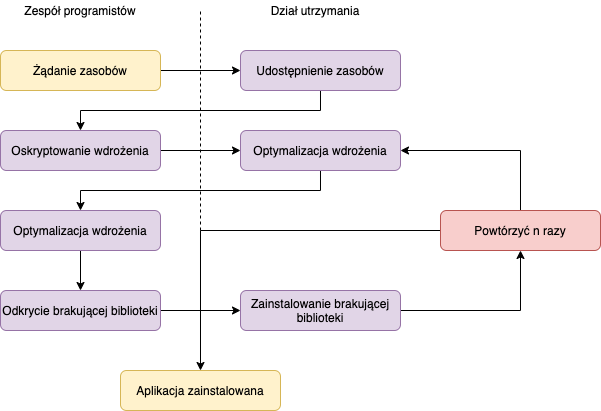
\includegraphics[width=.8\textwidth]{Chapters/Rozwiazanie/docker/proces-without-docker.png}
\caption{Przebieg tradycyjnego wdrożenia (bez Dockera).}
\label{fig:chapter3:proces-without-docker}
\end{figure}

\begin{figure}[!ht]
\centering
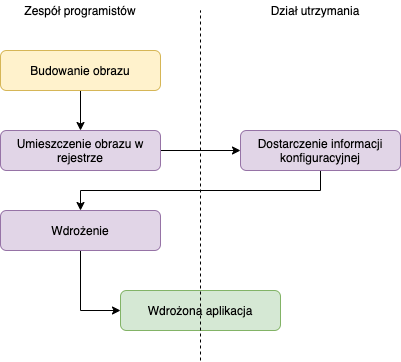
\includegraphics[width=.8\textwidth]{Chapters/Rozwiazanie/docker/proces-with-docker.png}
\caption{Przebieg wdrożenia z Dockerem.}
\label{fig:chapter3:proces-with-docker}
\end{figure}

%%%%%%%%%%%%%%%%%%%%%%%%%%%%%%%%%%%%%%%%%%%%%%%%

%%%%%%%%%%%%%%%%%%%%%%%%%%%%%%%%%%%%%%%%%%%%%%%%
\subsection{Czym Docker nie jest?}
Dzięki wykorzystaniu Dockera możliwe jest sprostanie wielu wyzwaniom, dla których tradycyjnie wykorzystywało się narzędzia innych kategorii. Szeroki zestaw możliwości często oznacza, że nie są dostępne bardzo specyficzne możliwości funkcjonalne. Na przykład w niektórych przypadkach pewne organizacje zauważą, że przy wykorzystaniu Dockera mogą zupełnie zrezygnować z narzędzi do zarządzania konfiguracją. Warto podkreślić, że Docker na pewno nie jest:

\begin{itemize}
    \item \textbf{Platformą do wirtualizacji (np. VMware, KVM)} - kontener nie jest maszyną wirtualną w tradycyjnym sensie. Maszyny wirtualne zawierają pełny system operacyjny działający pod kontrolą hiper nadzorcy zarządzanego przez system operacyjny serwera. Największą zaletą w porównaniu do sprzętowej wirtualizacji jest to, że w łatwy sposób można uruchomić wiele maszyn wirtualnych ze skrajnie różnymi systemami operacyjnymi na tym samym komputerze. Przy konteneryzacji zarówno główny system operacyjny, jaki i kontenery korzystają z tego samego jądra. To oznacza, że kontenery wykorzystują mniejszą ilość zasobów systemowych, ale muszą być oparte na tym samym systemie operacyjnym, zatem są mniej wymagające w stosunku do maszyn wirtualnych (Rysunek \ref{fig:chapter3:vm-vs-docker}).
    \item \textbf{Chmurą (np. Openstack, CloudStack)} - tak jak w przypadku wirtualizacji, wykorzystanie kontenerów wykazuje wiele podobieństw do korzystania z platform chmurowych. Oba te mechanizmy są tradycyjnie wykorzystywane, aby umożliwić horyzontalne skalowanie aplikacji w przypadku zmieniających się wymagań. Docker nie jest jednak platformą chmurową. Obsługuje jedynie wdrażanie, uruchamianie kontenerów i zarządzanie nimi na istniejących już komputerach z Dockerem. Nie pozwala na tworzenie nowych systemów (instancji), magazynów obiektów, urządzeń blokowych do przechowywania danych itp., jakie zazwyczaj zarządzane są przez platformę chmurową.
    \item \textbf{Zarządzaniem konfiguracją (np. Puppet, Chef) } - choć Docker znacząco usprawnia zarządzanie aplikacjami i ich zależnościami w organizacji, nie zastępuje bezpośrednio tradycyjnych systemów do zarządzania konfiguracją. W plikach Dockera definiuje się, jak kontener powinien wyglądać przy kompilacji, ale nie służą one do zarządzania późniejszym stanem kontenera i nie mogą być wykorzystywane do zarządzania systemem operacyjnym.
    \item \textbf{Frameworkiem do wdrażania (np. Capistrano, Fabric)} - Docker upraszcza wiele aspektów wdrażania aplikacji dzięki tworzeniu obrazów kontenerów, które zawierają wszystkie zależności aplikacji, w taki sposób, że mogą być one wdrożone w każdym środowisku bez modyfikacji. Docker nie może być jednak wykorzystany do automatyzacji złożonych procesów wdrażania. Potrzebne są nadal inne narzędzia pozwalające połączyć i zautomatyzować większe procesy.
    \item \textbf{Systemem do zarządzania obciążeniem (Mesos, Kubernetes, Swarm)} - dodatkowa warstwa koordynująca musi zostać wykorzystana do inteligentnego skoordynowania pracy większych grup serwerów z Dockerem, śledzenie stanu wszystkich serwerów oraz ich zasobów, a także rejestrowania działających kontenerów.
\end{itemize}

\begin{figure}[!ht]
\centering
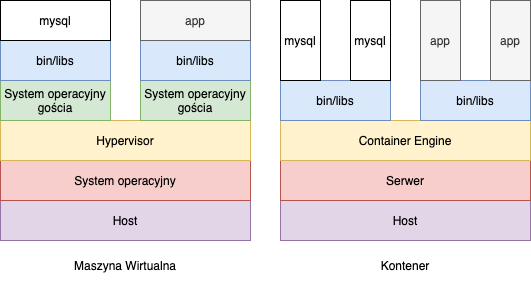
\includegraphics[width=.8\textwidth]{Chapters/Rozwiazanie/docker/vm-vs-docker.png}
\caption{Porównanie maszyny wirtualnej z kontenerem.}
\label{fig:chapter3:vm-vs-docker}
\end{figure}

\FloatBarrier

%%%%%%%%%%%%%%%%%%%%%%%%%%%%%%%%%%%%%%%%%%%%%%%%

%%%%%%%%%%%%%%%%%%%%%%%%%%%%%%%%%%%%%%%%%%%%%%%%
\section{Systemy do zarządzania kontenerami w środowisku chmurowym}
\label{sec:k8s}
Podczas wykorzystywania mechanizmu kontenerów w postaci silnika Docker inżynierowie zwrócili uwagę na problem koordynacji wielu pojedynczych serwerów z Dockerem i efektywnego wypełniania tych serwerów kontenerami. Powstało wiele narzędzi do zarządzania kontenerami w celu jak najefektywniejszego wykorzystania zasobów oferowanych przez klastry Dockerowe, takich jak Docker Swarm \cite{naik2016building}, Mesos \cite{mesos}, Centurion \cite{centurion} czy Kubernetes \cite{burns2018kubernetes}. W chwili obecnej na rynku komercyjnym liczą się tylko dwa rozwiązania: Docker Swarm oraz Kubernetes; ze znaczną przewagą tego drugiego, który obecnie dostarczany jest jako oprogramowanie usługa (ang. Software as a Service, w skrócie SaaS) przez wszystkich dostawców rozwiązań chmurowych \cite{chemashkinkubernetes}. 

\bigbreak
Kubernetes został zaprezentowany podczas konferencji DockerCon w 2014 roku przez firmę Google i od tego czasu dynamicznie się rozwija. Sama platforma dostępna jest dla wielu dystrybucji Linuxa. System do zarządzania kontenerami w środowisku chmurowym zapewnia między innymi:
\begin{itemize}
    \item \textbf{Detekcje nowych serwisów i balansowanie ruchu} - pozwala na udostępnienie kontenera, używając nazwy DNS lub swojego własnego adresu IP. Jeśli ruch przychodzący do kontenera jest zbyt duży, system może balansować obciążenie i przekierować ruch sieciowy, aby zapewnić stabilność całej instalacji (Rysunek \ref{fig:chapter3:lb}).
    \item \textbf{Zarządzenie obsługą składowania danych} - umożliwia automatyczne monitorowanie systemów składowania danych dowolnego typu.
    \item \textbf{Automatyczne wdrożenia i wycofywanie zmian} - można opisać oczekiwany stan instalacji, system sam zajmie się doprowadzeniem w sposób kontrolowany stanu faktycznego do stanu oczekiwanego. Przykładowo można zautomatyzować proces tworzenia nowych kontenerów na potrzeby wdrożenia oraz usuwania istniejących już kontenerów oraz zwalniania zasobów przez nie wykorzystywanych.
    \item \textbf{Automatyczne zarządzanie dostępnymi zasobami} - zadaniem administratora jest dostarczenie klastra maszyn, które można wykorzystać do uruchamiania zadań w kontenerach. Administrator określa zapotrzebowanie na moc procesora i pamięć RAM dla każdego z wykorzystywanych kontenerów. System sam rozmieszcza kontenery na maszynach w taki sposób, aby jak najlepiej wykorzystać dostarczone zasoby.
    \item \textbf{Samoczynne naprawianie} - system sam restartuje kontenery, które przestały działać, wymienia je na nowe i wymusza wyłączenie kontenerów, które nie działają, po czym poinformuje o dostępności nowych kontenerów, kiedy będą gotowe do działania. Dzięki czemu możliwe jest zbudowanie klastra, który będzie dostępny w dwóch osobnych lokalizacjach, tym samym lepiej wspierając wysoką dostępność (Rysunek \ref{fig:chapter3:ha}).
    \item \textbf{Zarządzanie informacjami poufnymi oraz konfiguracją} - system pozwala na składowanie oraz zarządzanie informacjami poufnymi, takimi jak hasła, tokeny API oraz klucze SSH. Informacje te mogą być dostarczane do aplikacji i zmieniane bez konieczności ponownego budowania obrazu kontenera i bez ujawniania poufnych danych w ogólnej konfiguracji oprogramowania.
\end{itemize}

\begin{figure}[!ht]
\centering
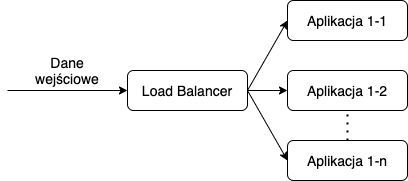
\includegraphics[width=.8\textwidth]{Chapters/Rozwiazanie/k8s/lb.png}
\caption{Wykorzystanie automatycznego mechanizmu równoważenia obciążenia (ang. Load Balancing).}
\label{fig:chapter3:lb}
\end{figure}

\begin{figure}[!ht]
\centering
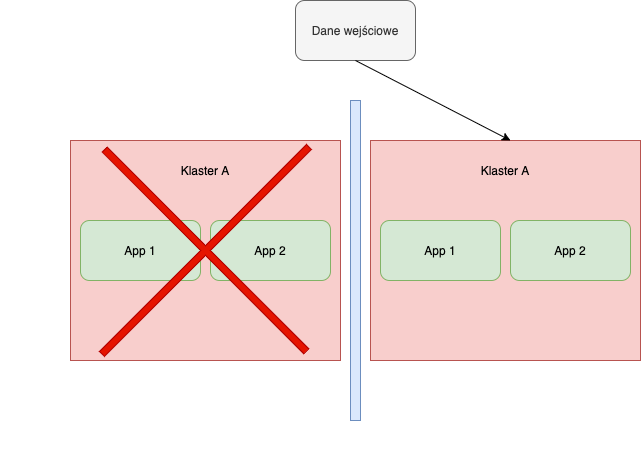
\includegraphics[width=.8\textwidth]{Chapters/Rozwiazanie/k8s/ha.png}
\caption{Mechanizm wysokiej dostępności.}
\label{fig:chapter3:ha}
\end{figure}

System zarządzania kontenerami dodatkowo:
\begin{itemize}
    \item Nie ogranicza typów aplikacji, które są obsługiwane. Celem systemu jest możliwość obsługi bardzo różnorodnego typu zadań, wliczając w to aplikacje bezstanowe (ang. stateless), aplikacje ze stanem (ang. stateful) i ogólne przetwarzanie danych.
    \item Nie oferuje wdrażania aplikacji wprost z kodu źródłowego i nie buduje aplikacji.
    \item Nie dostarcza warstwy aplikacyjnej, pośredniej (ang. middleware), np. broker wiadomości typu Rabbitmq, oraz funkcjonalności baz danych.
    \item Nie wymusza użycia konkretnych systemów zbierania logów, monitorowania ani ostrzegania.
    \item Nie dostarcza ani nie wymusza języka/systemu używanego do konfiguracji.
\end{itemize}

\bigbreak
Dzięki powyższym założeniom Kuberenetes pozwala na zbudowanie elastycznych i wysoko skalowalnych rozwiązań, dzięki czemu jest wykorzystywany również przez takie firmy jak Facebook, Twitter czy też Netflix \cite{vergilio2019non}.

%%%%%%%%%%%%%%%%%%%%%%%%%%%%%%%%%%%%%%%%%%%%%%%%

%%%%%%%%%%%%%%%%%%%%%%%%%%%%%%%%%%%%%%%%%%%%%%%%
\section{Opracowane oprogramowanie}
\label{sec:vmc}
Na potrzeby pracy autor stworzył oprogramowanie Centrum Zarządzania Podatnościami (ang. Vulnerability Management Center, w skrócie VMC), za pomocą którego przeprowadzono analizę zaproponowanych modeli zarządzania podatnościami \cite{vmcgithub}. W dalszej części pracy posługiwano się skrótem pochodzącym z języka angielskiego, gdyż jest on ogólnie przyjęty w opublikowanej przez autora literaturze. Oprogramowanie VMC wykorzystuje omówione wcześniej technologie w rozdziale \ref{sec:docker} oraz \ref{sec:k8s} i składa się z czterech głównych modułów: moduł pobierający informacje o podatnościach z publicznych baz danych (ang. Knowledge Collector), moduł pobierający informacje o zasobach infrastruktury teleinformatycznej (ang. Asset Collector), moduł pobierający informacje o wykrytych podatnościach w infrastrukturze teleinformatycznej (ang. Vulnerability Collector) oraz moduł obliczeniowy (ang. Processing Module). Rysunek \ref{fig:chapter3:vmc-arch} przedstawia architekturę VMC, które składają się na całość oprogramowania. Kolorem zielonym oznaczono komponenty, napisane przez autora pracy. Kolorem niebieskim komponenty, które są dostarczane przez firmy trzecie. Kolorem szarym dane wejściowe. Cały kod oprogramowania dostępny jest w publicznym repozytorium Github \cite{vmcgithub}. Dokładny opis instalacji oraz konfiguracji systemu dostępny jest w załącznikach dołączonych do niniejszej pracy.

\begin{figure}[!ht]
  \centering
  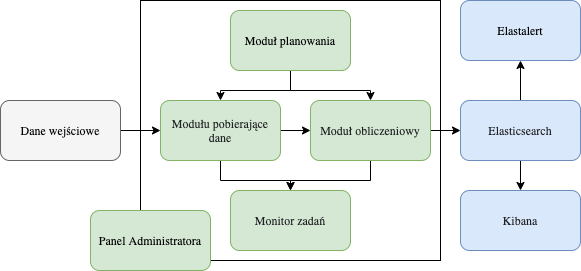
\includegraphics[width=.9\textwidth]{Chapters/Rozwiazanie/vmc/vmc-arch.png}
  \caption{Architektura VMC.}
  \label{fig:chapter3:vmc-arch}
\end{figure}

\bigbreak
Wszystkie moduły pracują niezależnie od siebie w myśl idei rozwiązań mikro serwisowych, komunikując się asynchronicznie za pomocą systemu kolejek \cite{johansson2020rabbitmq}. Dzięki czemu, w zależności od ilości danych przyjmowanych przez moduł, może być on skalowalny, niezależnie od pozostałych komponentów. 

\bigbreak
System konfigurowany jest z panelu administratora. Moduł planowania (ang. Scheduler) odpowiada za kolejność oraz czas pobierania danych z poszczególnych źródeł. Natomiast w monitorze zadań (ang. Task Monitor) można podejrzeć aktualny stan zadań wykonywanych w systemie. Dane przechowywane są w Elasticsearch \cite{gheorghe2015elasticsearch}, który umożliwia ich przetwarzanie w trybie pełnotekstowym, natomiast do warstwy prezentacji wyników wykorzystywane jest narzędzie Kibana \cite{gupta2015kibana}. Do implementacji niżej opisanych komponentów wykorzystany został język Python \cite{pilgrim2009dive} ze względu na jego elastyczność oraz możliwość wydajnego przetwarzania danych po stronie serwera. Cały projekt uwzględnia obsługę mulit-klientów (ang. tenants) oraz pozwala na pełną separację danych pomiędzy określonymi klientami. VMC działa w dwóch trybach: operacyjnym oraz historycznym. Tryb operacyjny pozwala użytkownikowi na podgląd wszystkich zaobserwowanych przez system zmian w czasie rzeczywistym, z kolei tryb historyczny umożliwia przeglądanie oraz wykonywanie operacji obliczeniowych na danych historycznych, poprawiając tym samym jakość i zakres analizy zdarzeń w systemie oraz w monitorowanej infrastrukturze teleinformatycznej.

\begin{figure}[thb]
\centering
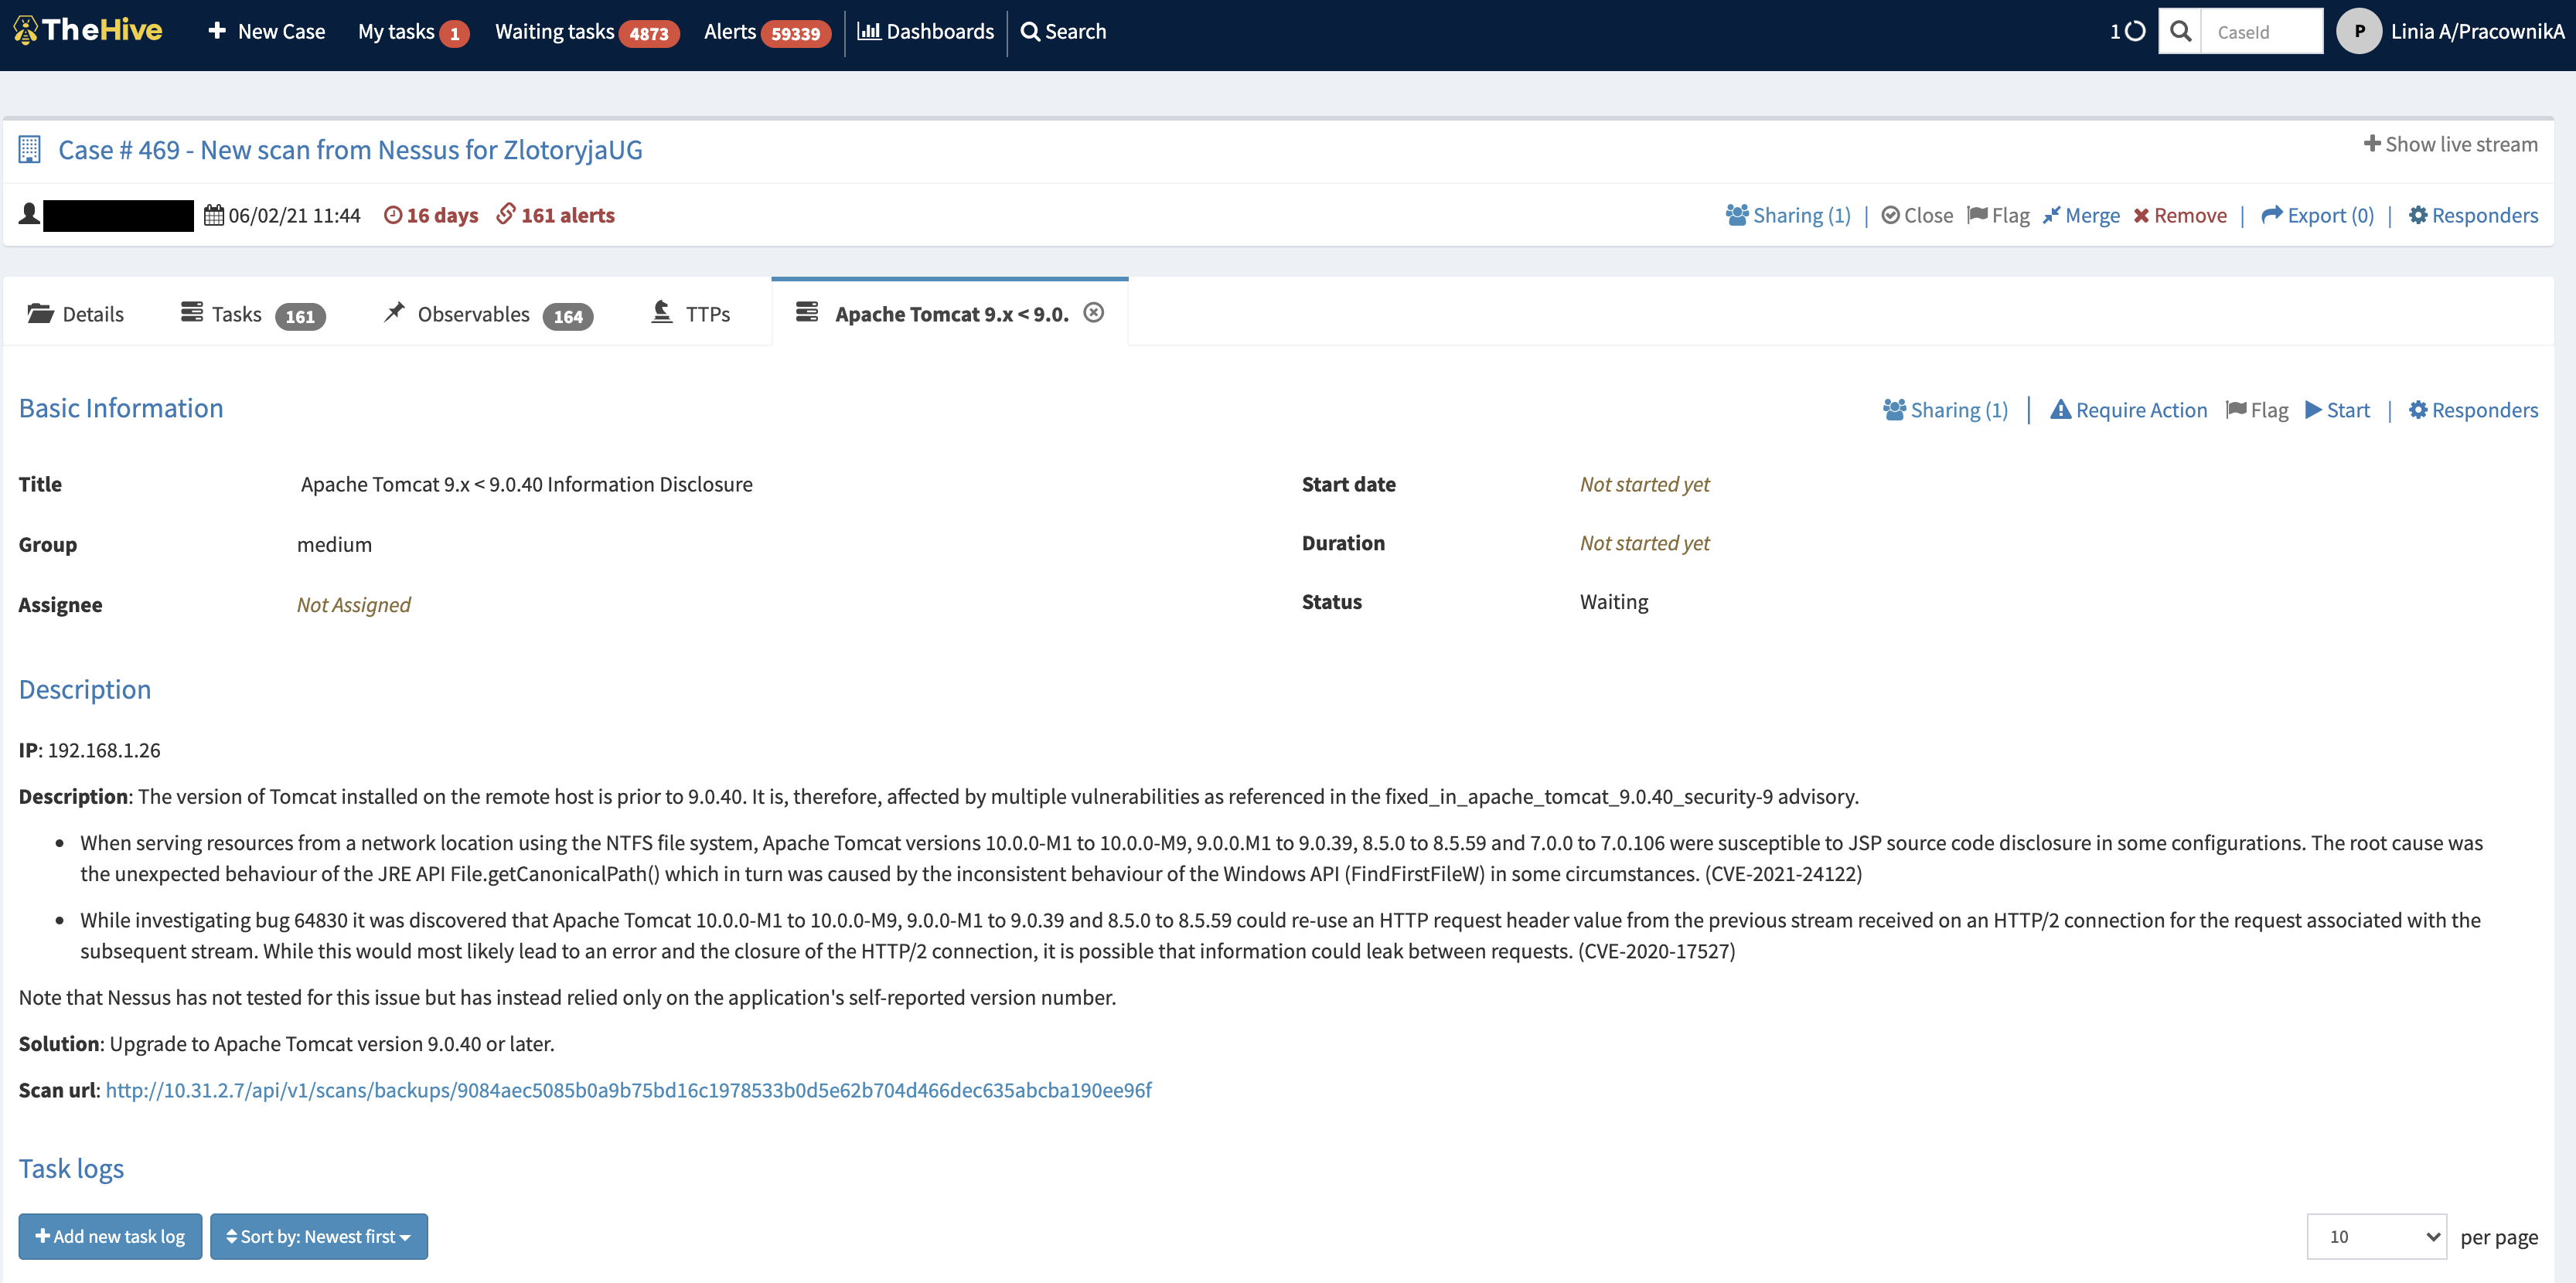
\includegraphics[width=\columnwidth]{Chapters/Rozwiazanie/vmc/hive-sample.png}
\caption{Przykładowy zrzut ekranu oprogramowania Hive zawierający informacje o podatności oraz sposobie jej naprawienia dla administratora zasobu.}
\label{fig:chapter3:hive-sample}
\end{figure}

\bigbreak
Dodatkowo istnieje możliwość wykorzystania modułu Elastalert \cite{elastalert} w celu monitorowania oraz alarmowania o odstępstwach od normy i anomaliach zachodzących w infrastrukturze lub też przygotowanie pełnej automatyzacji pozwalającej na bezpośrednie przesyłanie informacji o podatnościach do odpowiedniego administratora (Rysunek \ref{fig:chapter3:hive-sample}).

%%%%%%%%%%%%%%%%%%%%%%%%%%%%%%%%%%%%%%%%%%%%%%%%

%%%%%%%%%%%%%%%%%%%%%%%%%%%%%%%%%%%%%%%%%%%%%%%%
\subsection{Pobieranie informacji o podatnościach z zewnętrznych źródeł}
W celu rozwiązania problemu opisanego w podrozdziale \ref{sec:modele-zarzadzaia-podatnosciami} dotyczącego aktualizacji informacji dotyczących kategorii bazowej CVSS, która pomimo zapewnień standardu, w rzeczywistości może ulec zmianie, jeśli na jaw wyjdą nowe informacje, zaimplementowano moduł pobierania informacji o podatnościach z publicznych baz danych (ang. Knowledge Collector). Moduł ten odpowiada za pobieranie, aktualizację oraz normalizację informacji z publicznie dostępnych baz danych na temat znanych exploitów, słabości (ang. Common Weakness Enumeration, w skrócie CWE) \cite{martin2007common} oraz podatności (CVE) \cite{cvsspecification}. Do źródeł informacji należą między innymi NVD \cite{booth2013national} i Exploits Database \cite{exploitexploits}. Na rysunku \ref{lst:chapter3:cvedocument} przedstawiono przykładową znormalizowaną strukturę dla podatności, która zawiera również relacje do dokumentów zawierających informacje o publicznie dostępnych exploitach, jak i do informacji o identyfikacji podatnego oprogramowania (ang. Common Platform Enumeration, w skrócie CPE) \cite{buttner2009common}. W dokumencie przechowywany jest cały wektor składający się na ocenę bazową podatności w celu przyspieszenia obliczeń oraz umożliwieniu łatwiejszego wyszukiwania po jej charakterystycznych cechach, np możliwość zdalnego wykorzystania. Po przejściu procesu normalizacji zebrane informacje są możliwe do wyświetlenia w warstwie prezentacji (Rysunek \ref{fig:chapter3:kibana-sample}).

\begin{figure}[thb]
\centering
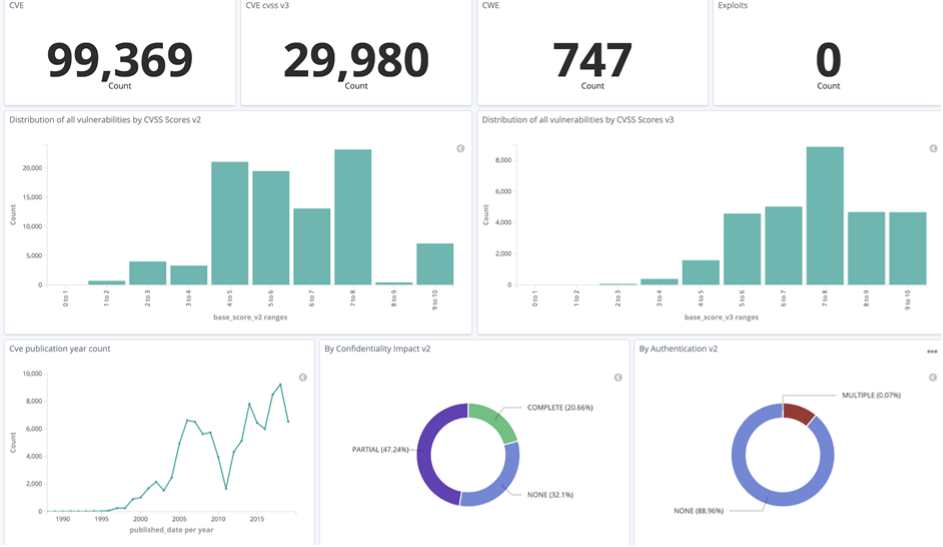
\includegraphics[width=\columnwidth]{Chapters/Rozwiazanie/vmc/kibana-sample.png}
\caption{Przykładowy zrzut ekranu oprogramowania VMC zawierający metryki.}
\label{fig:chapter3:kibana-sample}
\end{figure}

\newpage
\begin{lstlisting}[caption={Przykładowy dokument prezentujący informacje zebrane o podatnościach (ang. CVE) w Elasticsearch.}, label={lst:chapter3:cvedocument}, language=Python, captionpos=b]
class CveDocument:
    id
    base_score_v2
    base_score_v3
    summary
    access_vector_v2
    access_complexity_v2
    authentication_v2
    confidentiality_impact_v2
    integrity_impact_v2
    availability_impact_v2
    attack_vector_v3
    attack_complexity_v3
    privileges_required_v3
    user_interaction_v3
    scope_v3
    confidentiality_impact_v3
\end{lstlisting}

%%%%%%%%%%%%%%%%%%%%%%%%%%%%%%%%%%%%%%%%%%%%%%%%

%%%%%%%%%%%%%%%%%%%%%%%%%%%%%%%%%%%%%%%%%%%%%%%%
\subsection{Pobieranie informacji o zasobach infrastruktury ICT}
\label{sec:cia_desc}
Moduł pobierający informacje o zasobach (ang. Asset Collector) odpowiada za zarządzanie danymi dotyczącymi zasobów wykrytych oraz zdefiniowanych dla monitorowanej sieci \cite{weintraub2016security}. Wykorzystując skonfigurowany przez administratora interwał czasowy, moduł łączy się z bazą zasobów za pomocą interfejsu programistycznego aplikacji (ang. API), udostępnionego przez producentów oprogramowania, następnie stworzony parser wewnątrz VMC przekształca otrzymane informacje do znormalizowanej struktury dokumentu przechowywanego w bazie Elasticsearch.

\bigbreak
Moduł pobierający informacje o zasobach posiada dwa źródła danych. Pierwszym źródłem jest narzędzie Ralph \cite{ralph}, system spełniający wymagania sieci korporacyjnych pozwalających na zarządzanie cyklem życia poszczególnego komponentu środowiska ICT. Drugim źródłem danych jest skaner podatności, który oprócz skanowania posiada funkcjonalność wykrywania komponentów infrastruktury ICT. VMC za pomocą specjalnie przygotowanych reguł (załącznik nr Z.3) pozwala na poinformowanie operatora o niezgodnościach pomiędzy danymi zawartymi w bazie aktywów, a informacjami dostarczonymi z wynikami skanowania. Na rysunku \ref{fig:chapter3:ralph-sample} przedstawiono przykładowe informacje na temat zasobu wykorzystywanego przez organizację. Dodatkowo w bazie aktywów przechowywane są informacje wymagane z punktu widzenie procesu zarządzania podatnościami, takie jak wymagania ciągłości (ang Confidentiality, w skrócie C), integralności (ang. Integrity, w skrócie I) oraz dostępności (ang. Availability, w skrócie A). W kolejnych rozdziałach posłużono się skrótem pochodzącym z języka angielskiego CIA w odniesieniu do wymagań ciągłości, integralności oraz dostępności zasobów, gdyż jest on ogólnie przyjęty w literaturze.


\begin{figure}[thb]
\centering
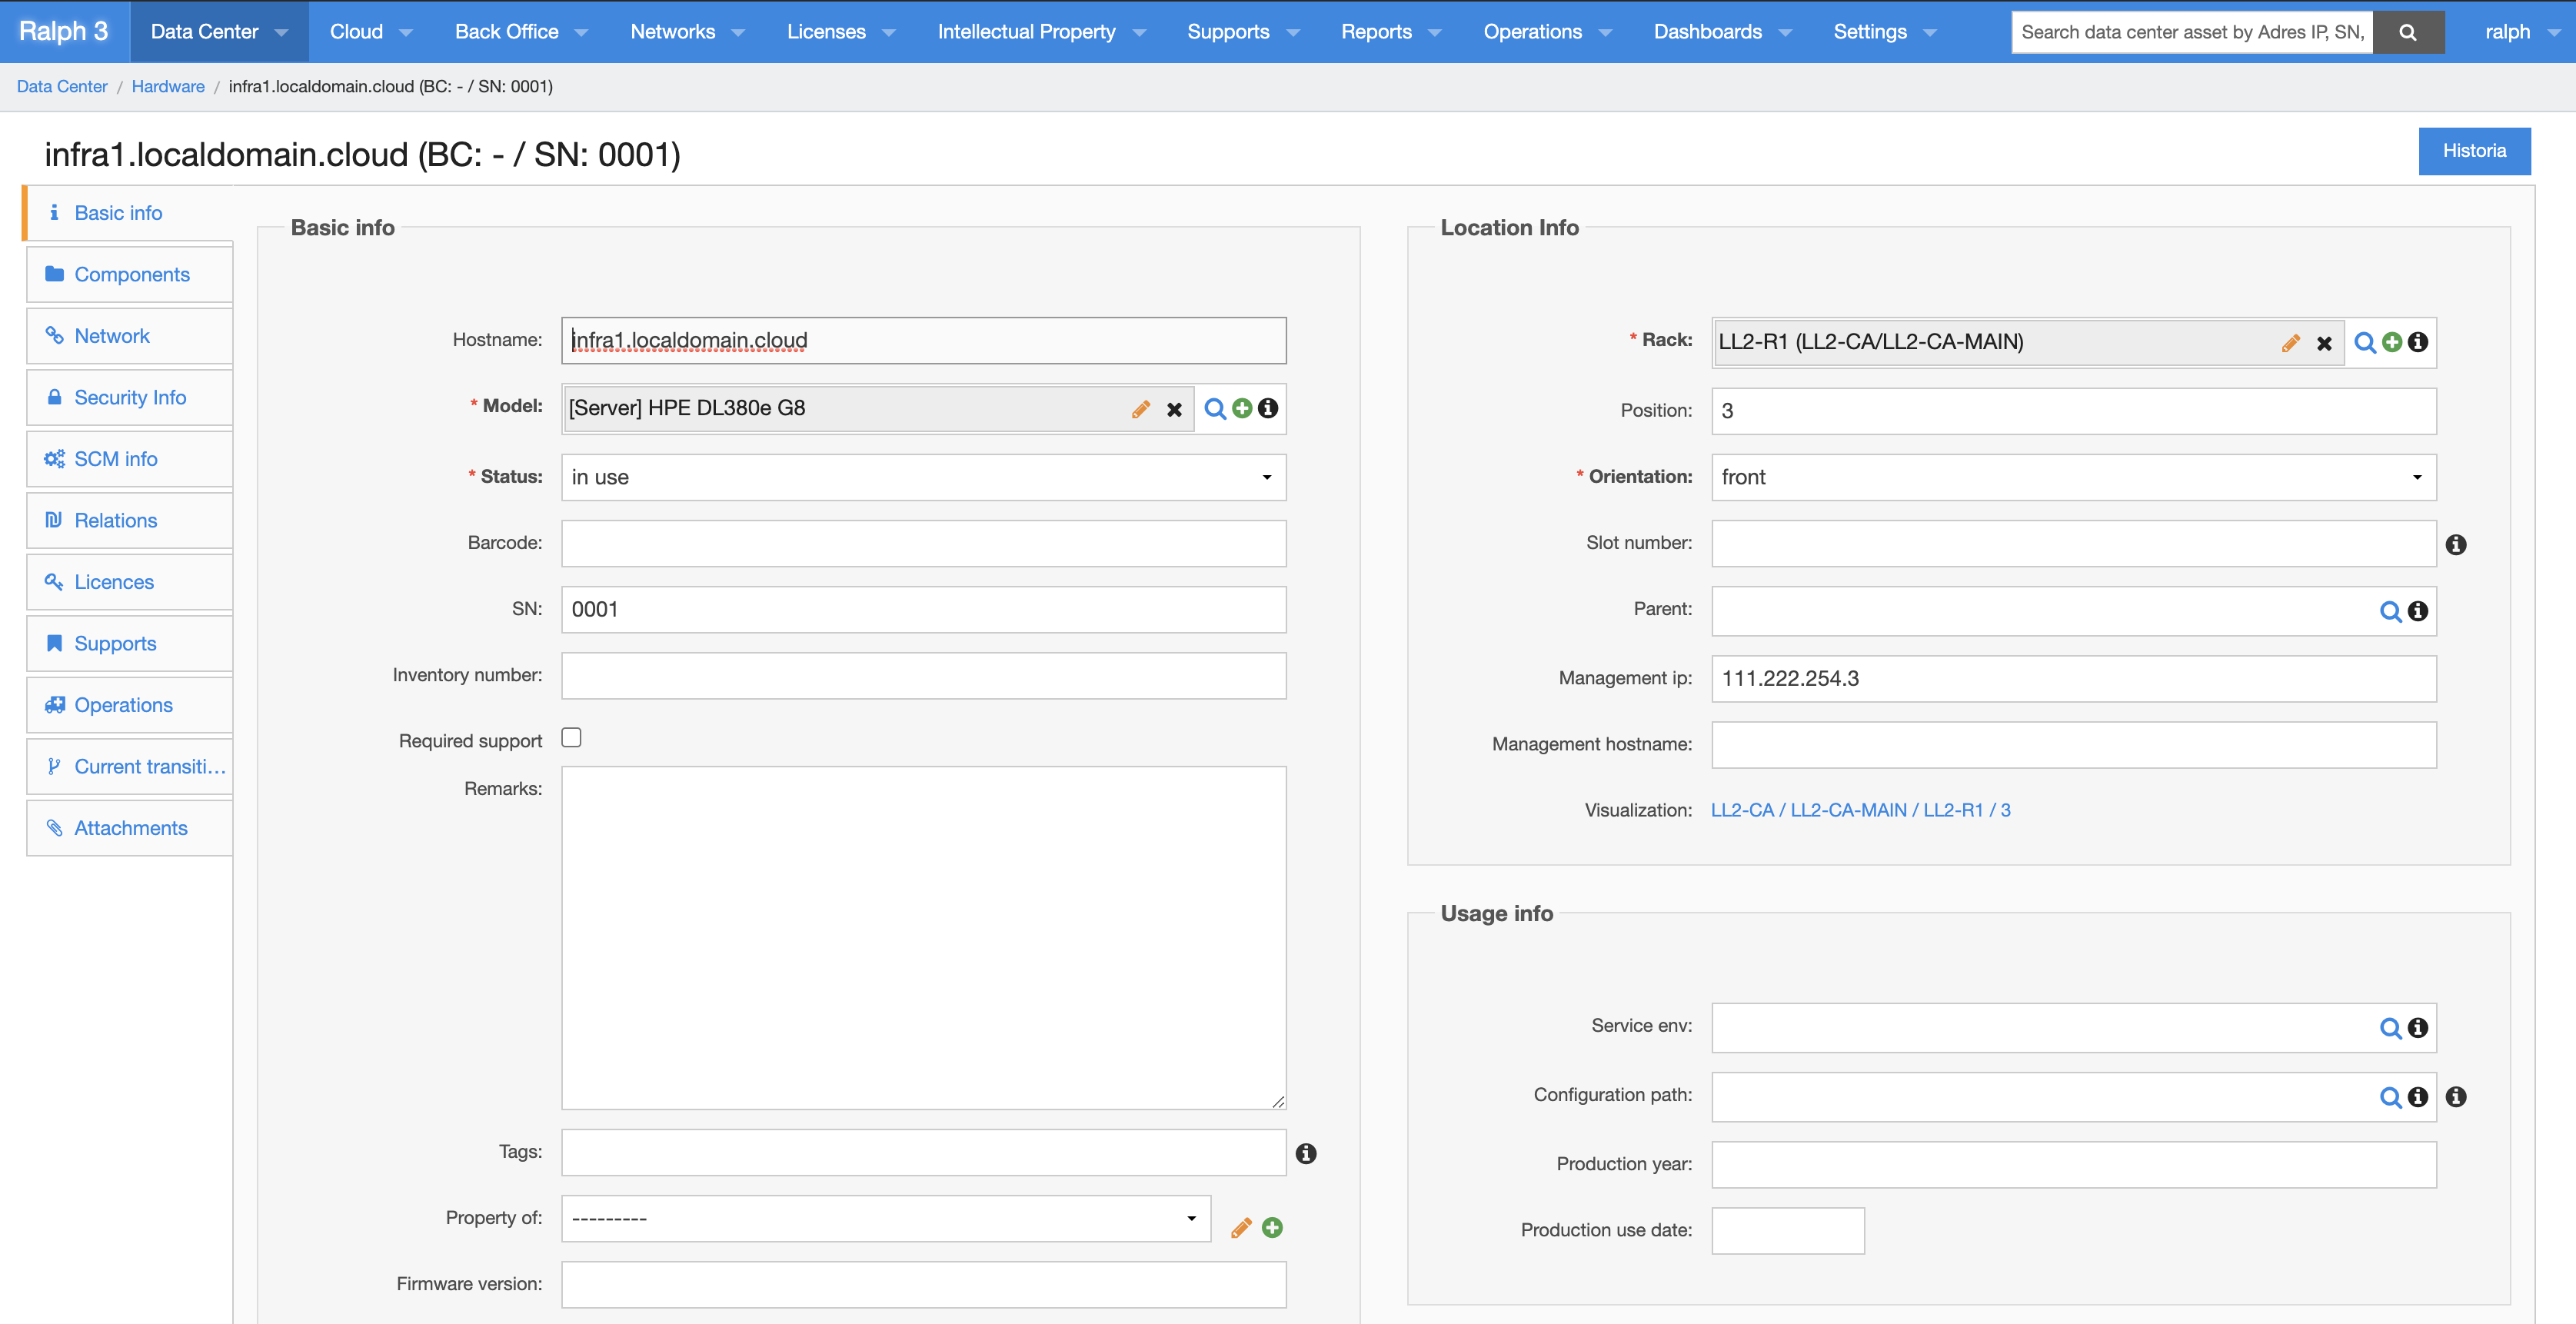
\includegraphics[width=\columnwidth]{Chapters/Rozwiazanie/vmc/ralph-sample.png}
\caption{Przykładowy zrzut ekranu z oprogramowania Ralph.}
\label{fig:chapter3:ralph-sample}
\end{figure}

\bigbreak
Informacje te umożliwiają analitykowi bezpieczeństwa na dostosowanie wyniku oceny podatności w zależności od znaczenia danego zasobu IT dla organizacji, mierzonego pod względem poufności, integralności i dostępności. Oznacza to, że jeśli zasób IT obsługuje funkcję biznesową, dla której dostępność jest najważniejsza, analityk może przypisać większą wartość dostępności w stosunku do poufności i integralności. Każdy wymóg bezpieczeństwa ma trzy możliwe wartości: Niski (ang. Low), Średni (ang. Medium) lub Wysoki (ang. High).

\bigbreak
Pełny wpływ na ocenę środowiskową jest określany przez odpowiednie ustawienia parametrów CIA (należy zauważyć, że ustawienia bazowe CVSS parametrów wpływu na poufność, integralność i dostępność nie ulegają zmianie). Oznacza to, że te parametry modyfikują ocenę środowiskową, zmieniając wagi (podstawowych) metryk wpływu poufności, integralności i dostępności. Na przykład parametr wpływu na poufność ma większą wagę, jeśli wymóg poufności jest wysoki. Podobnie parametr wpływu na poufność ma mniejszą wagę, jeśli wymóg poufności jest niski. Waga parametru wpływu na poufność jest neutralna, jeśli wymóg poufności jest średni. Ta sama logika jest stosowana do wymagań dotyczących integralności i dostępności.

\bigbreak
Listę możliwych wartości przedstawiono w Tabeli \ref{tab:chapter2:cia}. Dla zwięzłości ta sama tabela jest używana dla wszystkich trzech parametrów. Im wyższe wymagania dotyczące bezpieczeństwa, tym wyższa ocena podatności (wartość Średnia jest uważana za domyślną).

\begin{table}[tbh]
\caption{Możliwe wartości parametrów $CIA$}
\begin{center}
\label{tab:chapter2:cia}
\begin{tabular}{lll}
\hline \noalign {\smallskip}
\textbf{Symbol} & \textbf{Wartość} & \textbf{Znaczenie}    \\
\hline \noalign {\smallskip}
L   &   Niskie     & Utrata [poufności/integralności/dostępności] może \\
    &   (ang. Low) & mieć jedynie ograniczony negatywny wpływ na  \\
    &              & organizację lub osoby powiązane z organizacją  \\
    &              & (np. pracowników, klientów).\\
\hline \noalign {\smallskip}
M   & Średnie      & Utrata [poufności/integralności/dostępności] może \\
    & (ang. Medium)& mieć poważny negatywny wpływ na organizację \\
    &              & lub osoby powiązane z organizacją  \\
    &              & (np. pracowników, klientów).\\
\hline \noalign {\smallskip}
H   &  Wysokie     & Utrata [poufności/integralności/dostępności]  \\
    &  (ang. High) & prawdopodobnie będzie miała katastrofalny \\
    &              & negatywny wpływ na organizację lub osoby   \\
    &              & powiązane z organizacją (np. pracowników,  \\
    &              & klientów). \\
\hline \noalign {\smallskip}
ND (CVSS 2.0)& Niezdefiniowane   & Przypisanie tej wartości wskazuje, że nie ma  \\ 
X (CVSS 3.x) & (ang. Not Defined)& wystarczających informacji, aby wybrać \\
                  &                 & jedną z pozostałych wartości, i nie ma wpływu \\ 
                  &                 & na ogólną ocenę środowiskową, tzn. ma taki sam \\
                  &                 & wpływ na ocenę, jak przypisanie wartości średniej. \\
\hline \noalign {\smallskip}
\end{tabular}
\end{center}
\end{table}

%%%%%%%%%%%%%%%%%%%%%%%%%%%%%%%%%%%%%%%%%%%%%%%%

%%%%%%%%%%%%%%%%%%%%%%%%%%%%%%%%%%%%%%%%%%%%%%%%
\subsection{Pobierane informacji o wykrytych podatnościach w infrastrukturze ICT}
Moduł pobierający informacje o wykrytych podatnościach w infrastrukturze teleinformatycznej (ang. Vulnerability Collector) odpowiada za pobieranie, aktualizację oraz normalizację danych ze skanerów podatności Nessus \cite{beale2004nessus} oraz OpenVas \cite{rahalkar2019openvas}. Wykorzystując skonfigurowany przez administratora interwał czasowy, moduł łączy się ze skanerem za pomocą interfejsu programistycznego aplikacji (ang. API) udostępnionego przez producentów oprogramowania skanującego, następnie stworzony parser wewnątrz VMC przekształca otrzymane informacje do znormalizowanej struktury dokumentu przechowywanego w bazie Elasticsearch.

\bigbreak
W celu optymalizacji wyników podczas przetwarzania danych pomijane są podatności sklasyfikowane jako informacyjne. Z raportów dostarczanych ze skanerów podatności pobierane informacje zwierają numer portu, protokół, nazwa usługi, opis podatności oraz informacje, w jaki sposób podatność powinna zostać naprawiona, które stanowią rekomendacje dla osób implementujących mechanizmy naprawcze.


%%%%%%%%%%%%%%%%%%%%%%%%%%%%%%%%%%%%%%%%%%%%%%%%

%%%%%%%%%%%%%%%%%%%%%%%%%%%%%%%%%%%%%%%%%%%%%%%%
\subsection{Metoda optymalizacji obliczeń dla dużej ilości danych}
\label{sec:scaling}
Moduł obliczeniowy (ang. Processing Module) odpowiada za dokonywanie obliczeń oraz aktualizacje oceny wykrytych podatności z uwzględnieniem danych pozyskanych ze wcześniejszych modułów. Obliczenia uruchamiane są za każdym razem, kiedy zostanie wykryta zmiana w przechowywanych danych, pobranych za pomocą modułów opisanych w poprzednich podrozdziałach. Dodatkowo w celu przyspieszenia czasu obliczeń są one wykonywane niezależenie dla każdego klienta (ang. tenant), zachowując pełną separację informacji na temat zagrożeń. Dla każdej nowej lub zaktualizowanej podatności otrzymane wyniki obliczeń zapisywane są w odpowiednich polach dokumentu. Zapisywana jest również informacja, taka jak wektor oceny środowiskowej (ang. Environmental Score Vector), dzięki której można w łatwy sposób przeanalizować każdą z poszczególnych wartości mającą wpływ na końcową ocenę środowiskową.

\bigbreak
Wykorzystując architekturę systemu zaprojektowaną do pracy w chmurze, zaimplementowano algorytm pozwalający na automatyczne wykrywanie ilości dostępnych zasobów w celu ich optymalnego wykorzystania. Po pierwsze, algorytm pobiera liczbę podatności, które nie zostały naprawione lub nie zostały oznaczone jako zmitygowane (Rozdział \ref{sec:proces-zarzadzania-podatnosciami}). Następnie algorytm wyszukuje informacji o systemie, w którym to został uruchomiony, aby ocenić ilość dostępnych zasobów, które można wykorzystać do obliczeń. Podział zadań w zależności od dostępnych zasobów przypisuje się zgodnie z równaniem:

\begin{equation}
d = 
\begin{cases}
\label{eq:chapter3:split_alg}
v//t & \text{jeżeli } v//t \leq t \\
t & \text{w przeciwnym wypadku} 
\end{cases}
\end{equation}
gdzie:
\begin{description}
\item $d$ - ilość danych przetwarzanych przez jeden moduł obliczeniowy
\item $t$ - liczba dostępnych modułów obliczeniowych
\item $v$ - liczba podatności które zostały nienaprawione lub niezmitygowane
\end{description}

\bigbreak
Każdorazowo przed rozpoczęciem procesu obliczeń wykonywane jest powyższe równanie, pozwala to na zastosowanie mechanizmu skalowania horyzontalnego bez potrzeby restartu oprogramowania VMC.

\bigbreak
W celu przyspieszenia obliczeń wartości $TD$ każde zapytanie jest przechowywane w bazie on-memory Redis współdzielonej przez wszystkie moduły obliczeniowe \cite{chen2016towards}, dzięki czemu w rezultacie tylko jeden moduł zliczający wysyła zapytanie do bazy danych, a pozostałe pobierają wcześniej obliczoną informację. Wykonane obliczenia zapisywane są z wykorzystaniem osobnego wątku przy pomocy bulk method \cite{dixit2016elasticsearch}. Dzięki temu pętla obliczeniowa nie jest blokowana na czas zapisu wyników operacji w bazie Elasticsearch. Dodatkowo baza on-memory Redis służy do synchronizacji wszystkich zadań wykonywanych w systemie, pozwalając na tworzenie rozproszonych mutexów oraz semaforów \cite{yadav2015review}. W celu uniknięcia problemów związanych z zakleszczeniem lub zawieszeniem się zadań wykonywanych przez oprogramowanie VMC, zaimplementowano mechanizm kaskadowy, który na wykonanie konkretnego zadania ma trzy próby. Po trzech nie udanych próbach problem z opisem błędu zgłaszany jest do administratora oprogramowania VMC.

%%%%%%%%%%%%%%%%%%%%%%%%%%%%%%%%%%%%%%%%%%%%%%%%

%%%%%%%%%%%%%%%%%%%%%%%%%%%%%%%%%%%%%%%%%%%%%%%%
\subsection{Metoda określania potencjalnych szkód dodatkowych}
\label{sec:cdp}
Parametr określający potencjalne szkody dodatkowe (ang. Colleteral Damage Potential, w skrócie $CDP$) według opisu zamieszczonego w dokumentacji standardu CVSS 2.0 \cite{cvsspecification} odpowiedzialny jest za wskazywanie zasobów infrastruktury IT, które w wyniku chwilowej niedostępności mogą spowodować wysokie straty finansowe dla firmy. Możliwe wartości parametru $CDP$ wraz z opisem wymienione zostały w Tabeli \ref{tab:chapter2:cdp}. 


\bigbreak
Im wyższa wartość parametru, tym większy wpływ na potencjalne zagrożenia, co ma bezpośredni przekład na wyższą ocenę wykrytej podatności. Oczywiście każda organizacja musi sama określić dokładne znaczenie słów „niewielkie, umiarkowane, znaczące i katastrofalne”.

\bigbreak
Na potrzeby obliczeń zaproponowano rozwiązanie napisane w języku Python przedstawione na Rysunku \ref{lst:chapter3:cdp_alg}, gdzie $x$ reprezentuje monitorowany zasób IT, $cr$ jest wymogiem poufności (ang. Confidentiality Requirement), $ir$ oznacza wymóg integralności (ang. Integrity Requirement), $a$ ar oznacza wymóg dostępności (ang. Availability Requirement).

\begin{lstlisting}[caption={Algorytm określający wartość parametru. CDP dla monitorowanego zasobu.}, label={lst:chapter3:cdp_alg}, language=Python, captionpos=b]
 x = [cr, ir, ar]
 if x.count(HIGH) == 3:
        return HIGH
 if x.count(HIGH) > 0:
    return MEDIUM_HIGH

 if x.count(MEDIUM) > 0:
    return LOW_MEDIUM

 if x.count(LOW) > 1:
    return LOW

return NOT_DEFINED
\end{lstlisting}

\begin{table}[tbh]
\caption{Możliwe wartości parametru $CDP$}
\begin{center}
\label{tab:chapter2:cdp}
\begin{tabular}{lll}
\hline \noalign {\smallskip}
\textbf{Symbol} & \textbf{Wartość} & \textbf{Znaczenie}    \\
\hline \noalign {\smallskip}
N  & Żadne              & Brak wpływu na aktywa, produktywność lub przychody \\
   & (ang. None)        & organizacji.\\
\hline \noalign {\smallskip}
L  & Niskie             & Pomyślne wykorzystanie tej podatności może \\
   & (ang. Low)         & spowodować niewielkie  uszkodzenia fizyczne \\
   &                    & lub straty majątkowe. Może wystąpić niewielka \\
   &                    & utrata przychodów lub produktywności organizacji.\\
\hline \noalign {\smallskip}
LM & Niskie-Średnie     & Pomyślne wykorzystanie tej podatności może spowodować\\       
   & (ang. Low-Medium)  & umiarkowane uszkodzenia fizyczne lub straty majątkowe. \\
   &                    &  Może wystąpić umiarkowana utrata przychodów \\
   &                    & lub produktywności organizacji.\\
\hline \noalign {\smallskip}
MH & Średnio-Wysokie    & Pomyślne wykorzystanie tej podatności może spowodować \\
   & (ang. Medium-High) & znaczne szkody fizyczne lub straty materialne. Może \\
   &                    & dojść do znacznej utraty przychodów lub produktywności.\\
\hline \noalign {\smallskip}
H  & Wysokie            & Pomyślne wykorzystanie tej podatności może spowodować \\
   & (ang. High)        & katastrofalne fizyczne lub materialne uszkodzenia. \\ 
   &                    & Może nastąpić katastrofalna utrata  \\
   &                    & przychodów lub produktywności.\\
\hline \noalign {\smallskip}
ND &Niezdefiniowane     & Przypisanie tej wartości do metryki nie wpłynie \\
   & (ang. Not Defined) & na wynik końcowy. \\
\hline \noalign {\smallskip}
\end{tabular}
\end{center}
\end{table}

%%%%%%%%%%%%%%%%%%%%%%%%%%%%%%%%%%%%%%%%%%%%%%%%

%%%%%%%%%%%%%%%%%%%%%%%%%%%%%%%%%%%%%%%%%%%%%%%%
\subsection{Metoda określania dystrybucji podatności}
\label{sec:td}
Parametr określający dystrybucje podatności (ang. Target Distribution, w skrócie $TD$) według opisu zamieszczonego w dokumentacji standardu CVSS 2.0 \cite{cvsspecification} jest specyficzny dla monitorowanego środowiska i odpowiedzialny za wskazanie procentu monitorowanych zasobów IT podatnych na wykryte zagrożenia. Możliwe wartości dla parametru $TD$ są wymienione w Tabeli \ref{tab:chapter2:td}. Im większy odsetek systemów podatnych, tym wyższy wynik końcowy oceny środowiskowej.

\bigbreak
Algorytm obliczający parametr $TD$ został zaimplementowany jako stosunek liczby nienaprawionych i niezmitygowanych podatności do liczby monitorowanych zasobów:

\begin{equation}
TD(x) = 
\begin{cases}
0.00 & x < 0.01 \\
0.25 & 0.01 \leq x < 0.25 \\
0.75 & 0.25 \leq x < 0.75 \\
1.00 & 0.75 \leq x \leq 1.00 \\
\end{cases}
\end{equation}

Gdzie:
\begin{equation}
    x = v / a 
\end{equation}

W powyższym równaniu $v$ reprezentuje liczbę nienaprawionych i niezmitygowanych podatności (Rozdział \ref{sec:proces-zarzadzania-podatnosciami}), natomiast $a$ reprezentuje liczba monitorowanych zasobów w środowisku ICT.

\begin{table}[tbh]
\caption{Możliwe wartości parametru $TD$}
\begin{center}
\label{tab:chapter2:td}
\begin{tabular}{lll}
\hline \noalign {\smallskip}
\textbf{Symbol} & \textbf{Wartość} & \textbf{Znaczenie}    \\
\hline \noalign {\smallskip}
N & Żadne & Nie istnieją żadne systemy docelowe lub cele są tak wysoce      \\
  & (ang. None) & wyspecjalizowane, że istnieją tylko w warunkach \\
  &             & laboratoryjnych. Efektywnie zagrożone jest 0\% środowiska. \\
\hline \noalign {\smallskip}
L & Niskie     & Pomyślne wykorzystanie tej podatności może spowodować \\
  & (ang. Low) & niewielkie uszkodzenia fizyczne lub straty finansowe. \\  
  &            &  Może wystąpić niewielka utrata przychodów  \\
  &            & lub produktywności organizacji. \\
\hline \noalign {\smallskip}
M & Średnie    & Pomyślne wykorzystanie tej podatności może spowodować \\       
& (ang. Medium)& umiarkowane uszkodzenia fizyczne lub straty finansowe.\\
  &           & Może wystąpić umiarkowane utrata przychodów \\
  &           & lub produktywności organizacji.\\
\hline \noalign {\smallskip}
H & Wysokie    & Pomyślne wykorzystanie tej podatności może spowodować \\
  & (ang. High)& katastrofalne fizyczne lub straty finansowe. Może \\ 
  &            & nastąpić katastrofalna utrata przychodów lub produktywności. \\
\hline \noalign {\smallskip}
ND&Niezdefiniowane& Przypisanie tej wartości nie wpłynie na wynik końcowy. \\
  &(ang. Not Defined) & \\
\hline \noalign {\smallskip}
\end{tabular}
\end{center}
\end{table}

%%%%%%%%%%%%%%%%%%%%%%%%%%%%%%%%%%%%%%%%%%%%%%%%

%%%%%%%%%%%%%%%%%%%%%%%%%%%%%%%%%%%%%%%%%%%%%%%%
\section{Metoda konwersji CVSS 2.0 do CVSS 3.x}
\label{sec:ml}
Nie wszystkie publicznie znane podatności mają ocenę bazową według CVSS 3.x, czyli najnowszym i najbardziej zaawansowanej wersji standardu CVSS (Rozdział \ref{sec:modele-zarzadzaia-podatnosciami}). Wynika to z dużej luki czasowej między publikacją standardów CVSS 2.0 i CVSS 3.x, dużej liczbie wykrytych i opublikowanych podatności oraz istotnymi różnicami w sposobie określania właściwości wektorowych oceny bazowej. W związku z tym organizacje korzystające z CVSS do ustalania priorytetów podatności używają obu wersji standardu CVSS i zrezygnowały z pełnego przejścia na CVSS 3.x. W celu rozwiązania niniejszego problemu braku oceny bazowej CVSS 3.x dla wszystkich podatności i umożliwienia wykonania priorytetyzacji wszystkich podatności za pomocą proponowanego modelu środowiskowego CVSS 3.x (Rysunek \ref{fig:chapter1:vm-model-cvss3e}) wykorzystano rozwiązanie zaproponowane przez autora niniejszej rozprawy, natomiast zaimplementowane przez doktora Macieja Nowaka. 

\bigbreak
Konwersja oceny bazowej CVSS 2.0 na CVSS 3.x wymaga jednoczesnego rozwiązania wielu problemów statystycznych. W pozyskiwanych danych wejściowych występuje niezrównoważenie (ang. imbalance data) powodujące trudności w fazie uczenia, co skutkuje obniżeniem zdolności predykcyjnych. Dodatkowo wynik końcowy CVSS 3.x powiązany jest funkcją opisaną 8 parametrami, z których każdy może przyjmować jedną z kilku wartości (od 2 do 4), ale pozyskanie samych parametrów tworzących wektor CVSS 2.0 dla większości przypadków okazuje się niewystarczające.

\bigbreak
Liczba kombinacji występująca w wektorze używanym do wyliczenia oceny bazowej CVSS 3.x wynosi 2592, natomiast wartość tego wektora zawiera się w przedziale 0 – 10 z rozdzielczością wynoszącą 0.1. Inaczej mówiąc, na podstawie zbioru uczącego, finalnie trzeba dokonać klasyfikacji każdego wektora testującego do jednej ze stu klas przypisanych do oceny bazowej CVSS 3.x.

\bigbreak
Zgodnie z dokumentacją opisującą ocenę bazową CVSS 3.x wyliczona wartość oceny bazowej przyjmuje jedną z pięciu kategorii (ang. Qualitative Severity Rating Scale). Kategorie te również nie są tak samo liczne, a ich proporcja wynosi odpowiednio: 1 : 39 : 30 : 20 : 10 (informacyjna : niska : średnia : wysoka : krytyczna).  W praktyce wskazana asymetria zakresu kategorii oznacza, że jeśli ocena bazowa CVSS dla wersji 3.x przyjmuje wartość 0, to wykonując konwersję z oceny bazowej CVSS 2.0 na 3.x, nie możemy popełnić żadnego błędu. Odchylenie od oceny bazowej CVSS 3.x dla kategorii krytycznej musi być z kolei mniejsze niż dla wysokiej, itd. 

\bigbreak
Podejście do rozwiązania problemu konwersji oceny bazowej składa się z kilku kroków. Po pierwsze, z pozyskanych danych należy odpowiednio wyselekcjonować zbiory trenujące tak, aby uzyskać jak najwyższą sprawność (ang. accuracy) klasyfikacji dla każdego z ośmiu parametrów tworzących wektor CVSS 3.x. W tym celu zastosowano dwie koncepcje wykorzystujące medianę i korelację wektorów, z których pierwsza, poprzez zastosowanie undersamplingu prowadzi do pełnego zbalansowania danych, natomiast druga statystycznie wiąże wszystkie parametry wektora CVSS 3.x, pozwalając na pozyskanie wektorów uczących z pewną stałą regułą. Kolejnym krokiem jest wyodrębnienie cech (ang. relevant features) z zestawu pozyskanych wektorów, używając analizy głównych komponentów (ang. Principal Component Analysis, w skrócie PCA), a następnie wykonanie uczenia pod nadzorem (ang. supervised learning methods) za pomocą różnych algorytmów. Porównano i przeanalizowano wiele metod statystycznej klasyfikacji (ag. statistical classification methods), takich jak maszyna wektorów podpierających (ang. Support Vector Machine, w skrocie SVM), naiwny klasyfikator Bayesa (ang. Naive Bayes classifier) oraz k-najbliższych sąsiadów (ang. K-nearest neighbor, w skrócie kNN). Po ustaleniu, które metody najskuteczniej klasyfikują w obrębie danego parametru wektora CVSS 3.x, przeprowadzano próby klasyfikacji przy zwiększeniu liczby wektorów zbioru testującego ze 100 do 1000. To ostatecznie pozwoliło wybrać najlepszych kandydatów i odpowiednio zoptymalizować modele klasyfikacji.

\bigbreak
Wstępne badania wykazały, że oryginalne wektory oceny bazowej CVSS 2.0 zostały nieprawidłowo zmapowane do 3.x, więc oryginalny wektor oceny bazowej CVSS 2.0 został rozszerzony o dodatkowe 50, 100, 500 i 1000 elementów. Dodatkowe elementy są uzyskiwane z opisów podatności i obliczane poprzez podzielenie liczby wystąpień słów kluczowych przez 100. Przetwarzanie tekstu zostało wykonane przy użyciu biblioteki Natural Language Toolkit (NLTK) \cite{bird2009natural}. Skrypty i dane wejściowe zostały umieszczone w repozytorium otwartego dostępu \cite{cvss-2-extended-vector-database-github}. Ponieważ uzyskane dane są niezrównoważone, zastosowano metodę undersamplingu opisaną w \cite{Nowak-cldd-2021}. Badania zostały przeprowadzone z następującymi algorytmami uczenia maszynowego:
\begin{itemize}
\item Algorytm k-najbliższych sąsiadów (ang. k-Nearest Neighbors, w skrócie kNN) z metryką euklidesową (E) i podobieństwem cosinusowym (C).
\item Naiwny klasyfikator Bayesa (ang. Naive Bayes classifier, w skrócie NB).
\item Probabilistyczna sieć neuronowa (ang. Probabilistic Neural Network, w skrócie PNN),
\item Miękkie niezależne modelowanie według analogii klas (ang. Soft Independent Modeling of Class Analogy, w skrócie SIMCA),
\item Maszyna wektorów podpierających z funkcją jądrową (ang. Kernel support vector machine, w skrócie KSVM) w dwóch konfiguracjach — z liniową funkcją jądra i korzystającą z jądra uczącego z radialną funkcją bazową (TGRBF) \cite{nowak2019recognition}. KSVM TRGBF w pętli uczenia wykorzystuje 2-krotną walidację krzyżową (2-krotne CV), współczynnik błędnej klasyfikacji (ang. Misclassification Ratio, w skrócie MCR), algorytm NM z zestawem 50 punktów początkowych i kNN z metryką cosinusową (C) do końcowej klasyfikacji nierozpoznanych próbek. Dodatkowo w przypadku KSVM TRGBF zastosowano podejście One-vs-One (OvO) dla parametrów o co najmniej 3 klasach.
\end{itemize}

Optymalizacja parametrów algorytmów uczenia maszynowego została przeprowadzona na podstawie pięciokrotnej walidacji krzyżowej zbioru 100 elementowego. Procedura testowa została powtórzona 10 razy i pozwoliła na określenie uśrednionych wartości współczynnika błędnych klasyfikacji (ang. Misclassification Ratio, w skrócie MCR), precyzji (ang. precision), czułości (ang. recall) i F1 (średnia harmoniczna pomiędzy precyzją (ang. precision) i czułością (ang. recall)). W kolejnym etapie wykonana została ocena dokładności klasyfikacji dla wybranych algorytmów na podstawie 30 prób przeprowadzonych z zbiorami testowymi zawierającymi losowo wybranymi 1000 elementowymi wektorami. Parametry algorytmu zostały ponownie zoptymalizowane w celu uzyskania maksymalizacji dokładności klasyfikacji przy jak najmniejszym rozrzucie wyników. Opisane w rozdziale 4 wyniki zostały potwierdzone za pomocą zbioru testującego składającego się z zbioru 71 000 wektorów.

%%%%%%%%%%%%%%%%%%%%%%%%%%%%%%%%%%%%%%%%%%%%%%%%

%%%%%%%%%%%%%%%%%%%%%%%%%%%%%%%%%%%%%%%%%%%%%%%%
\begin{comment}
\section{Metoda pomiaru zakresu oraz liczby zmian w ocenie podatności}
\label{sec:metoda_pomiar_zakres_oraz_liczba_zmian}
W celu zmierzenia zakresu oraz liczby zmian w ocenie podatności a tym samym wpływu parametrów środowiskowych $CIA$, $TD$ oraz $CDP$ na ocenę bazową CVSS, posłużono się równaniem przedstawionym poniżej:

\begin{equation}
d = X_{CVSS_{Base}} - X_{CVSS_{Env}}
\end{equation}

Gdzie wartość $d$ to różnica pomiędzy otrzymanymi ocenami, $X_{CVSS_{Base}}$  to ocena bazowa otrzymana ze skanera Nessus, $X_{CVSS_{Env}}$ to ocena środowiskowa obliczona za pomocą oprogramowania VMC. Otrzymana ujemna wartość $d$ wskazuje, że ocena środowiskowa została obniżona w stosunku do oceny bazowej, analogicznie, wartość dodatnia $d$ informuje, że ocena środowiskowa jest wyższa od ceny bazowej. W celu określenia liczby zmian w priorytetyzacji podatności dla standardu CVSS 2.0 oraz CVSS 3.x, zliczono wszystkie unikalne wystąpienia otrzymanych wartości $d$.
\end{comment}


\chapter{Środowiska badawcze}
\label{sec:desc_env_all}
W poprzednim rozdziale omówiono sposoby implementacji w opracowanym oprogramowaniu VMC rozwiązania problemów stawianych przez tezę pracy (Rozdział \ref{sec:zakres-i-teza-pracy}). Zostały w nim przedstawione również wykorzystane nowoczesne technologie, takie jak konteneryzacja (Rozdział \ref{sec:docker}) oraz systemy do zarządzania kontenerami w środowisku chmurowym (Rozdział \ref{sec:k8s}), które dzięki zastosowaniu mechanizmu opisanego w rozdziale \ref{sec:scaling} pozwalają na optymalizacje obliczeń dla dużej ilości danych.

\bigbreak
W tym rozdziale przedstawiono opis trzech niezależnych, rzeczywistych środowisk teleinformatycznych, wykorzystanych do analiz umożliwiających weryfikacje poprawności założonej tezy (Rozdział \ref{sec:zakres-i-teza-pracy}). 
Opisy dotyczą podstawowych, ilościowych wyników związanych z liczbą wykrytych podatności przez oprogramowanie skanujące. Wykorzystane środowiska teleinformatyczne A, B i C są środowiskami rzeczywistymi, dlatego wszystkie adresy IP zostały zanimizowane. Dla środowiska teleinformatycznego A oprócz otrzymania raportów z wykrytymi podatnościami za pomocą oprogramowania Nessus \cite{beale2004nessus} otrzymano informacje na temat ustawień parametrów środowiskowych $CIA$, które szerzej opisane zostały w rozdziale \ref{sec:cia_desc}. Dla środowiska teleinformatycznego B otrzymano tylko raport z wykrytymi podatnościami za pomocą oprogramowania Nessus. Dla środowiska teleinformatycznego C otrzymano raport z wykrytymi podatnościami za pomocą oprogramowania Nessus oraz ogólne informacje dotyczące wag skanowanych zasobów. Niniejszy rozdział podzielony jest na pięć podrozdziałów. Pierwsze trzy podrozdziały poświęcone są opisom danych pochodzących ze środowisk teleinformatycznych. W czwartym podrozdziale przedstawiona została konfiguracja sprzętu oraz oprogramowania wykorzystana do zbadania modeli zarządzania podatnościami (Rozdział \ref{sec:modele-zarzadzaia-podatnosciami}), ponieważ właściciele zasobów udostępniający informacje na temat swoich środowisk teleinformatycznych nie wyrazili zgody na przetwarzanie danych w środowisku chmurowym. W ostatnim, piątym podrozdziale omówiono konfiguracje środowiska wykorzystaną do zbadana przyrastającej ilości danych na parametr $T_{VMC}$ (Rozdział \ref{sec:modele-ewaluacji-efektywnosci}), który jest miernikiem skuteczności działania rozwiązań przedstawionych w rozdziałach \ref{sec:docker}, \ref{sec:k8s}, \ref{sec:scaling}.

\section{Opis badanego środowiska teleinformatycznego A}
\label{sec:desc_a}
W środowisku teleinformatycznym A dostępne są 23 serwery odpowiadające za dostarczanie usług, takich jak portale internetowe dla wewnętrznych potrzeb organizacji, zawierające 36 podatności wykrytych przez skaner Nessus. Dodatkowo skaner zgłosił 322 podatności o kategorii informacyjnej, które zawierają w znacznej większości informacje na temat konfiguracji samego procesu skanowania oraz wykrytych otwartych portów i usług. Skan został wykonany bez autoryzacji, to znaczy bez logowania na skanowane zasoby. Skan został przeprowadzony w dniu 11.02.2021 i trwał 3 godziny.

\bigbreak
Tabela \ref{tab:chapter5:env_a:detected_vulns_nessus} przedstawia dokładną liczbę wykrytych podatności przez skaner Nessus z rozróżnieniem na oba standardy. Różnica pomiędzy liczbą wskazywaną przez raport Nessus a liczbą podatności według CVSS wynika z grupowania przez oprogramowanie skanujące niektórych CVE do jednej kategorii, przykładowo ujęta w raporcie podatność “134944 - PHP 7.3.x < 7.3.16 Multiple Vulnerabilities” posiada przypisane trzy CVE, mianowicie CVE-2020-7064, CVE-2020-7065, CVE-2020-7066. Różnica pomiędzy liczbą otrzymanych ocen bazowych CVSS 2.0 oraz CVSS 3.x wynika z problemu braku oceny dla tej samej podatności według obu standardów. Problem opisany został szerzej w rozdziale \ref{sec:modele-zarzadzaia-podatnosciami}.

\begin{table}[tbh]
\caption{Liczba wykrytych podatności według oceny bazowej CVSS dla środowiska A.}
\begin{center}
\label{tab:chapter5:env_a:detected_vulns_nessus}
\begin{tabular}{ccc}
\hline \noalign {\smallskip}
 & ocena bazowa CVSS 2.0 & ocena bazowa CVSS 3.x \\
\hline \noalign {\smallskip}
\textbf{Liczba Podatności}  &  41    & 27 \\
\hline \noalign {\smallskip}
\end{tabular}
\end{center}
\end{table}

\bigbreak
Rysunek \ref{fig:chapter5:env_a:env_stats} przedstawia histogram podziału kategorii podatności według ocen bazowych CVSS 2.0 oraz 3.x z której wynika, że znacząca większość wykrytych podatności, bo aż 83\% dla CVSS 2.0 oraz 52\% dla CVSS 3.x, są podatnościami o kategorii średniej (Rozdział \ref{sec:cvss_2_standard}, \ref{sec:cvss_3_standard}). Dokładna analiza wyników skanowania, podział kategorii oraz szacowana liczba roboczogodzin została przedstawiona w rozdziale czwartym.

\begin{figure}[!ht]
\centering
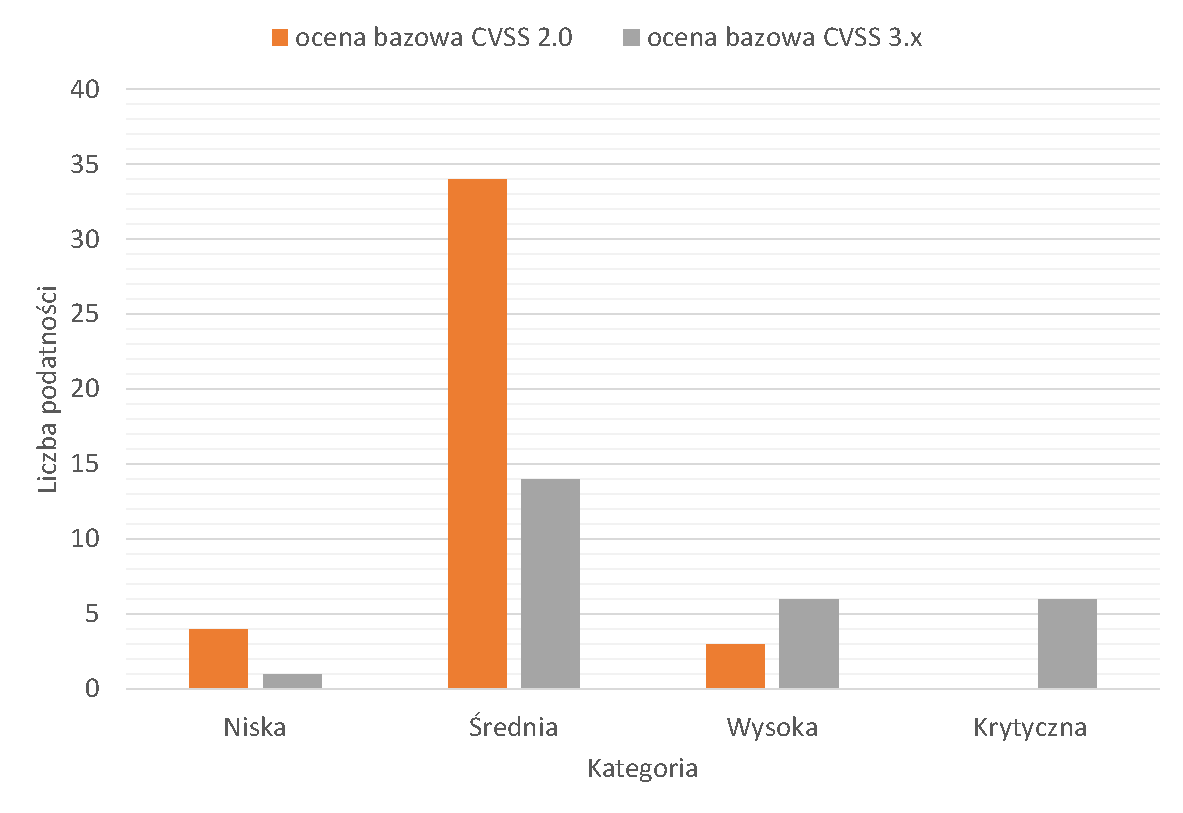
\includegraphics[width=.8\textwidth]{Chapters/Srodowiska/env_A/env_a_stats.pdf}
\caption{Histogram kategorii podatności z podziałem na oceny bazowe CVSS 2.0 i 3.x dla środowiska A.}
\label{fig:chapter5:env_a:env_stats}
\end{figure}


\bigbreak
Tabela \ref{tab:chapter5:env_a:cia} przedstawia rozkład parametrów środowiskowych $CIA$, który został dostarczony przez administratorów środowiska teleinformatycznego A. Dotyczy 5 skanowanych serwerów, co odpowiada 21.47\% wszystkich zasobów w testowanym środowisku. W związku z tym parametry $CIA$ ustawione są jako niezdefiniowane dla pozostałych 78.26\% serwerów. Parametr dotyczący wymagań dostępności (ang. Availability) ustawiony jest jako: wysoki dla 3 elementów sieci; średni dla 2 elementów sieci; co odpowiada 13.04\% i 8.7\%. Parametr dotyczący wymagań integralności (ang. Integrity) ustawiony jest jako: wysoki dla 1 serwera; średni dla 1 serwera, co odpowiada 4.35\%.

\begin{table}[tbh]
\caption{Rozkład parametrów $CIA$ dla środowiska A.}
\begin{center}
\label{tab:chapter5:env_a:cia}
\begin{tabular}{lllll}
\hline \noalign {\smallskip}
\textbf{Nazwa}           & Niska   & Średnia & Wysoka & Niezdefiniowana   \\
\hline \noalign {\smallskip}
\textbf{Poufność} &   13.04\%  &  4.35\%    & 4.35\%      &   78.26\% \\
\textbf{Integralność}       &   13.04\%  &  4.35\%    & 4.35\%      &   78.26\%  \\
\textbf{Dostępność}    &       0\%  &   8.7\%   & 13.04\%      &   78.26\%  \\
\hline \noalign {\smallskip}
\end{tabular}
\end{center}
\end{table}

%%%%%%%%%%%%%%%%%%%%%%%%%%%%%%%%%%%%%%%%%%%%%%%%

%%%%%%%%%%%%%%%%%%%%%%%%%%%%%%%%%%%%%%%%%%%%%%%%
\section{Opis badanego środowiska teleinformatycznego B}
\label{sec:desc_b}
W środowisku teleinformatycznym B dostępne jest 36 serwerów z różnymi niesprecyzowanym usługami, świadczonymi dla pracowników organizacji. Informacje o usługach uruchomionych na wskazanych serwerach są nieistotne z punktu widzenia przeprowadzonych analiz, które opisane zostały w rozdziale czwartym oraz piątym. Środowisko teleinformatyczne B zawiera 85 podatności wykrytych przez skaner Nessus. Dodatkowo skaner zgłosił 615 podatności o kategorii informacyjnej, które zawierają w znacznej większości informacje na temat konfiguracji samego procesu skanowania oraz wykrytych otwartych portów i usług. Skan został przeprowadzony w dniach od 04.05.2021 do 05.05.2021 i trwał 19 godzin.

\bigbreak
Tabela \ref{tab:chapter5:env_b:detected_vulns_nessus} przedstawia liczbę podatności wykrytych przez skaner Nessus z rozróżnieniem na oba standardy. Tak samo jak w przypadku środowiska teleinformatycznego A, różnica pomiędzy liczbą wskazywaną przez raport Nessus a liczbą podatności według oceny bazowej CVSS wynika z grupowania podatności przez oprogramowanie skanujące niektórych CVE do jednej kategorii. Różnica pomiędzy liczbą CVSS 2.0 oraz CVSS 3.x wynika z problemu braku oceny bazowej dla tej samej podatności według obu standardów. Problem opisany został szerzej w rozdziale \ref{sec:modele-zarzadzaia-podatnosciami}.

\begin{table}[tbh]
\caption{Liczba wykrytych podatności według oceny bazowej CVSS dla środowiska B.}
\begin{center}
\label{tab:chapter5:env_b:detected_vulns_nessus}
\begin{tabular}{ccc}
\hline \noalign {\smallskip}
                &  ocena bazowa CVSS 2.0 & ocena bazowa CVSS 3.x\\
\hline \noalign {\smallskip}
\textbf{Liczba Podatności} &      104       & 54    \\
\hline \noalign {\smallskip}
\end{tabular}
\end{center}
\end{table}

\bigbreak
Rysunek \ref{fig:chapter5:env_a:env_stats} przedstawia histogram podziału kategorii podatności według oceny bazowej CVSS 2.0 oraz 3.x, z której wynika, że znacząca większość wykrytych podatności, bo aż 90\% dla CVSS 2.0 oraz 55\% dla CVSS 3.x, są podatnościami o kategorii średniej (Rozdział \ref{sec:cvss_2_standard}, \ref{sec:cvss_3_standard}). Dokładne omówienie wyników skanowania, podział kategorii oraz szacowana liczba roboczogodzin zostaną przedstawione w rozdziale czwartym.

\bigbreak
Dla środowiska teleinformatycznego B, administrator nie dostarczył żadnych informacji, z których możliwe byłoby określenie wartości parametrów środowiskowych $CIA$ (Rozdział \ref{sec:cia_desc}), w związku z czym wytworzone oprogramowanie VMC na potrzeby przeprowadzonych analiz dla wszystkich wartości parametrów przyjęto wartość niezdefiniowaną, która jak opisano w rozdziale \ref{sec:cia_desc}, nie ma wpływu na otrzymaną ocenę środowiskową. 

\begin{figure}[!ht]
\centering
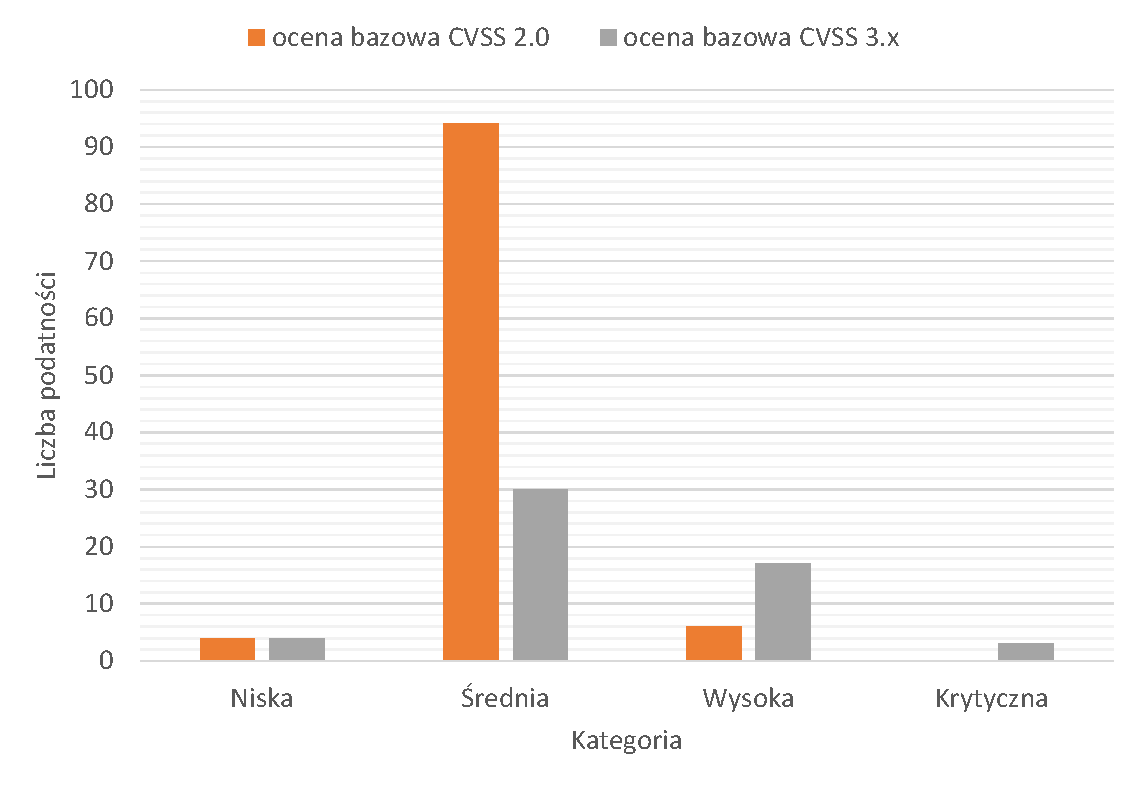
\includegraphics[width=.8\textwidth]{Chapters/Srodowiska/env_B/env_b_stats.pdf}
\caption{Histogram kategorii podatności z podziałem na ocenę bazową CVSS 2.0 i 3.x dla środowiska B.}
\label{fig:chapter5:env_b:env_stats}
\end{figure}



%%%%%%%%%%%%%%%%%%%%%%%%%%%%%%%%%%%%%%%%%%%%%%%%

%%%%%%%%%%%%%%%%%%%%%%%%%%%%%%%%%%%%%%%%%%%%%%%%
\section{Opis badanego środowiska teleinformatycznego C}
\label{sec:desc_c}
W środowisku teleinformatycznym C dostępne są 2 062 urządzenia sieciowe, czyli cała wewnętrzna infrastruktura organizacji, dla której skaner Nessus wykrył 2 949 podatności. Dodatkowo skaner zgłosił 16 640 podatności o kategorii informacyjnej, które zawierają w znacznej większości informacje na temat konfiguracji samego procesu skanowania oraz wykrytych otwartych portów i usług. Skan został częściowo wykonany z autoryzacją, mianowicie skaner posiadał możliwość zalogowania się na 41 urządzeniach sieciowych, co stanowi niecałe 2\% badanego środowiska. Skan został przeprowadzony w dniach od 26.04.2021 do 27.04.2021 i trwał 23 godziny. 

\bigbreak
Tabela \ref{tab:chapter5:env_c:detected_vulns_nessus} przedstawia liczbę podatności wykrytych przez skaner Nessus z rozróżnieniem na oba standardy. Tak samo jak w przypadku środowiska teleinformatycznego A i B, różnica pomiędzy liczbą wskazywaną przez raport Nessus a liczbą podatności według oceny bazowej CVSS wynika z tego, że Nessus grupuje niektóre CVE do jednej kategorii. Różnica pomiędzy liczbą ocen bazowych CVSS 2.0 oraz CVSS 3.x wynika z problemu braku oceny dla tej samej podatności według obu standardów. Problem opisany szerzej został w rozdziale \ref{sec:modele-zarzadzaia-podatnosciami}.

\begin{table}[tbh]
\caption{Liczba wykrytych podatności według oceny bazowe CVSS dla środowiska C.}
\begin{center}
\label{tab:chapter5:env_c:detected_vulns_nessus}
\begin{tabular}{ccc}
\hline \noalign {\smallskip}
   & ocena bazowa CVSS 2.0 & ocena bazowa CVSS 3.x \\
\hline \noalign {\smallskip}
\textbf{Liczba Podatności}   &      10 078 &         9 730 \\
\hline \noalign {\smallskip}
\end{tabular}
\end{center}
\end{table}

\bigbreak
Rysunek \ref{fig:chapter5:env_c:env_stats} przedstawia histogram kategorii podatności według ocen bazowych CVSS 2.0 oraz CVSS 3.x. Na podstawie wyników z rysunku \ref{fig:chapter5:env_c:env_stats} można stwierdzić, że znacząca większość wykrytych podatności, bo aż 65\% dla CVSS 2.0 oraz 46\% dla CVSS 3.x, są podatnościami o kategorii średniej (Rozdział \ref{sec:cvss_2_standard}, \ref{sec:cvss_3_standard}).


\begin{figure}[!ht]
\centering
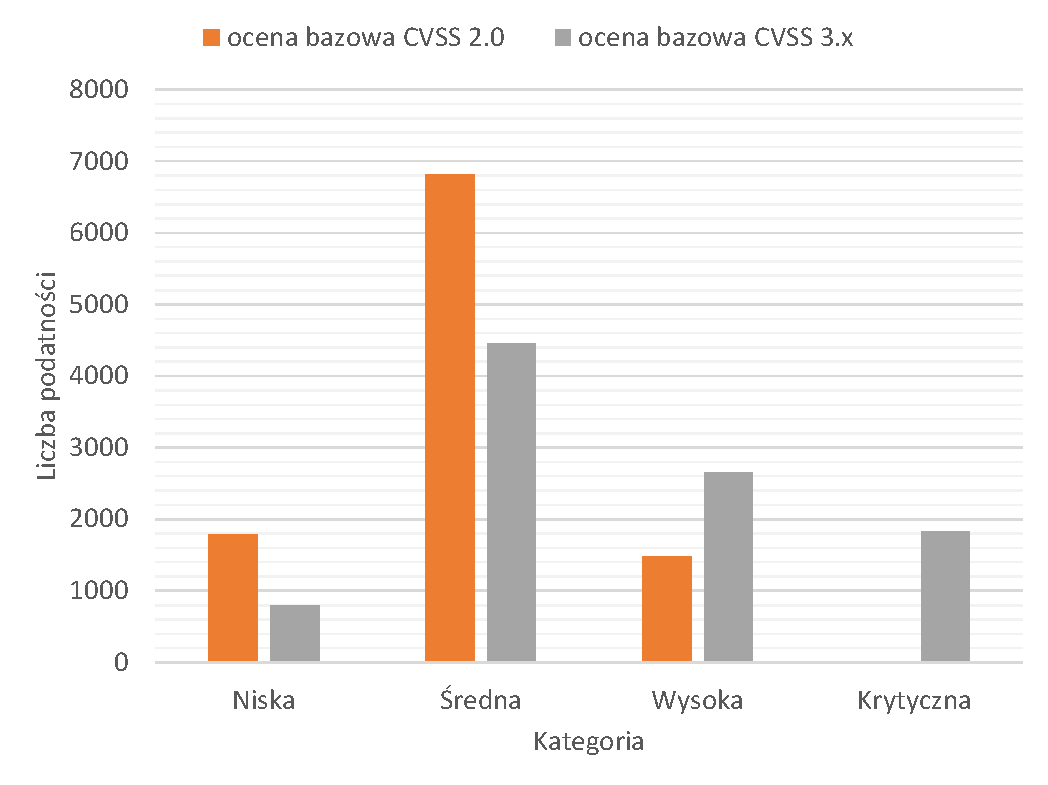
\includegraphics[width=.7\textwidth]{Chapters/Srodowiska/env_C/env_c_stats.pdf}
\caption{Histogram kategorii podatności z podziałem na oceny bazowe CVSS 2.0 i 3.x dla środowiska C.}
\label{fig:chapter5:env_c:env_stats}
\end{figure}


\bigbreak
Dla środowiska teleinformatycznego C administrator dostarczył tylko ogólne informacje dotyczące wagi skanowanych zasobów (podział: niskie, średnie, krytyczne), z których wynika, że 217 urządzeń określonych jest wagą krytyczną, 790 oznaczonych wagą średnią, 851 wagą niską z punktu widzenia organizacji. Dla 204 zasobów administrator nie dostarczył żadnych informacji. Całościowy rozkład wag zasobów przedstawiony został na rysunku \ref{fig:chapter5:env_c:os_cia}.

\begin{figure}[!ht]
\centering
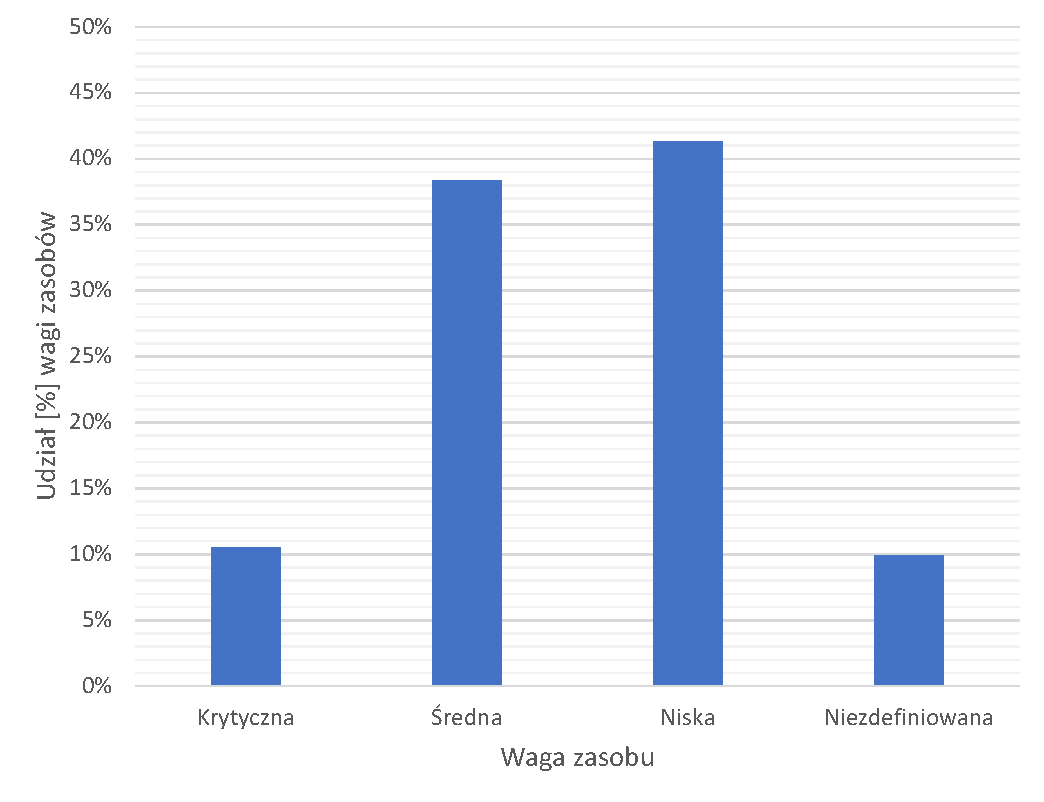
\includegraphics[width=.7\textwidth]{Chapters/Srodowiska/env_C/os_cia.pdf}
\caption{Histogram wag zasobów dla środowiska C.}
\label{fig:chapter5:env_c:os_cia}
\end{figure}

%%%%%%%%%%%%%%%%%%%%%%%%%%%%%%%%%%%%%%%%%%%%%%%%

%%%%%%%%%%%%%%%%%%%%%%%%%%%%%%%%%%%%%%%%%%%%%%%%
\section{Środowisko badawcze do pomiaru wpływu zmiany priorytetyzacji}
\label{sec:desc_pio}
Ponieważ organizacje, które udostępniły informacje na temat swoich środowisk teleinformatycznych (A, B, C) oraz wykrytymi w nich podatnościami za pomocą oprogramowania Nessus, nie wyraziły zgody na przetwarzanie danych w infrastrukturze zewnętrznej (w chmurze). W celu przeprowadzenia analiz potwierdzających tezę opisaną w rozdziale \ref{sec:zakres-i-teza-pracy}, zaimplementowane oprogramowanie na potrzeby pracy (Rozdział \ref{sec:vmc}) zostało uruchomione na komputerze MacBook Pro 2018 z procesorem 2.6 GHz Intel Core i7 oraz 32 GB 2400 MHz DDR4, wykorzystując technologię Docker (Rozdział \ref{sec:docker}) w następującej konfiguracji:
\begin{itemize}
\item Moduł obliczeniowy (ang. Processing Module) 
\item Monitor zdań (ang. Task monitor)
\item Panel Administratora (ang. Admin Panel)
\item Moduł pobierający informacje o zasobach infrastruktury teleinformatycznej (ang. Asset Collector)
\item Moduł pobierający informacje o wykrytych podatnościach w infrastrukturze teleinformatycznej (ang. Vulnerability Collector)
\item Baza danych PostgreSQL \cite{postgresql1996postgresql} - przechowywanie konfiguracji VMC 
\item Baza danych MariaDB \cite{bartholomew2012mariadb} - przechowywanie informacji o zasobach IT
\item Ralph \cite{ralph} - Panel administracyjny bazy zasobów IT 
\item Rabbitmq \cite{johansson2020rabbitmq} - system kolejkowy używany do komunikacji pomiędzy modułami VMC 
\item Baza Redis \cite{chen2016towards} - in-memory używana do przechowywania częściowych obliczeń i synchronizacji modułów VMC 
\item Elasticsearch  \cite{dixit2016elasticsearch} - baza tekstowa przechowująca informacje o wszystkich podatnościach 
\item Kibana \cite{gupta2015kibana} - graficzny interfejs pozwalający w łatwy sposób wyszukiwać wyniki oraz tworzyć metryki 
\end{itemize}

%%%%%%%%%%%%%%%%%%%%%%%%%%%%%%%%%%%%%%%%%%%%%%%%

%%%%%%%%%%%%%%%%%%%%%%%%%%%%%%%%%%%%%%%%%%%%%%%%
\section{Środowiska badawcze do analizy skalowalności rozwiązania}
\label{sec:desc_skalowalnosc}
W celu przeprowadzenia analiz dotyczących wpływu przyrastającej ilości przetwarzanych danych na parametr $T_{VMC}$ wprowadzonym w rozdziale \ref{sec:modele-ewaluacji-efektywnosci}. Zaimplementowane na potrzeby pracy oprogramowanie (\ref{sec:vmc}) zostało uruchomione w Microsoft Azure\textsuperscript{\textregistered} Free Tier subscription \cite{microsoft-fre-tier}. Ze względu na napotkane ograniczenia licencyjne, dotyczące możliwości wykorzystywania zasobów na bezpłatnej subskrypcji w jednym centrum danych, wykorzystano dwa niezależne centra danych: US West USA i US West USA 2, które w komunikacji między sobą wykazują średnie opóźnienie na poziomie 22 ms \cite{microsoft-latency}. W regionie US West 2 uruchomiono klaster kubernetes (\ref{sec:k8s}) składający się z 2 serwerów, każdy z procesorami 2$\times$ Intel Xeon\textsuperscript{\textregistered} E5-2673 v3 (Haswell) 2,4 GHz i 7 GB pamięci RAM z następującymi usługami:

\begin{itemize}
\item Moduł obliczeniowy (ang. Processing Module) 
\item Monitor zdań (ang. Task monitor)
\item Panel Administratora (ang. Admin Panel)
\item Moduł pobierający informacje o zasobach (ang. Asset Collector) 
\item Baza danych PostgreSQL \cite{postgresql1996postgresql} - przechowywanie konfiguracji VMC
\item Baza danych MariaDB \cite{bartholomew2012mariadb} - przechowywanie informacji o zasobach IT
\item Ralph \cite{ralph} - Panel administracyjny bazy zasobów IT
\item Rabbitmq \cite{johansson2020rabbitmq} - system kolejkowy używany do komunikacji pomiędzy modułami VMC
\item Baza Redis \cite{chen2016towards} - in-memory używana do przechowywania częściowych obliczeń i synchronizacji modułów VMC
\end{itemize}

\bigbreak
W regionie USA West został uruchomiony klaster Elasticsearch składający się z 2 serwerów, każdy o konfiguracji 1 $\times$ CPU Intel Xeon\textsuperscript{\textregistered} E5-2673 v3 (Haswell) 2,4 GHz, 3,5 GB pamięci RAM. Pomiędzy regionami utworzono sieć wirtualną (VLan).

\chapter{Wpływ parametrów na zmianę oceny oraz kategorii podatności}
W tej części rozprawy analizowany jest wpływ parametrów środowiskowych na ocenę bazową CVSS, a tym samym na możliwości zmiany kategorii krytyczności podatności, na przykład z kategorii niskiej na krytyczną. Możliwość zmiany kategorii krytyczności podatności z niskiej na krytyczną pozwala na stwierdzenie mówiące o ryzyku nienaprawienia podatności z niedoszacowaną oceną lub naprawienia podatności z przeszacowaną oceną za pomocą modeli zarządzania podatnościami wykorzystującymi ocenę bazową CVSS (Rysunek \ref{fig:chapter1:vm-model-cvss2}, \ref{fig:chapter1:vm-model-cvss3}). W związku z tym, że wykrywane jest coraz więcej podatności w środowiskach teleinformatycznych, istnieje możliwość, że podatność niedoszacowana, posiadająca klasyfikacje niską, nigdy nie zostanie naprawiona przez administratorów, ponieważ podatności o wyższej klasyfikacji zawsze będą naprawiane w pierwszej kolejności. W konsekwencji nienaprawiona podatność niedoszacowana o klasyfikacji niskiej, która w rzeczywistości mająca klasyfikację na przykład średnią wpływa na czas ekspozycji podatności w systemie, która może zostać wykorzystana przez atakującego. Należy jednak pamiętać, że wpływ parametrów środowiskowych CVSS może nie być brany pod uwagę w procesie napraw podatności w przypadku małych organizacji, gdzie liczba skanowanych zasobów i wykrytych podatności jest niewielka. Natomiast w każdej organizacji osoba odpowiedzialna za proces zarządzania podatnościami musi podjąć decyzję czy uważa, że jego organizacja wymaga usprawnień w postaci uwzględniania parametrów środowiskowych CVSS.

\bigbreak
Do przeprowadzenia analizy wybrano po jednej podatności reprezentującej każdą klasyfikację krytyczności według oceny bazowej dla standardu CVSS 2.0 (Tabela \ref{tab:cvss_criticality_2}) oraz 3.x (Tabela \ref{tab:cvss_criticality_3}). Wybrane podatności zostały wykryte w środowisku teleinformatycznym A za pomocą oprogramowania skanującego Nessus. Dla każdej kategorii krytyczności wyniki analizy uporządkowano w następujący sposób. Najpierw porównano wpływ parametrów środowiskowych na ocenę bazową CVSS 2.0. W tym celu napisany został program, za pomocą którego obliczono wszystkie możliwe do uzyskania wartości oceny środowiskowej CVSS 2.0 dla każdej kombinacji parametrów środowiskowych $CIA$, $TD$, $CDP$ (Załącznik Z1), a następnie przeanalizowano liczbę oraz zakres zmian w kategoriach podatności. Wzięto pod uwagę wadę oceny środowiskowej CVSS 2.0 dotyczącej parametru $TD$, który służy do ustalania liczby systemów wrażliwych na daną podatność, przez co znacząco zaniża oceny wszystkich wykrytych podatności. Dlatego też w dalszej części dokonano analizy wpływu parametrów środowiskowych na ocenę bazową CVSS 3.x. W tym celu również został napisany program, za pomocą którego obliczono wszystkie możliwe do uzyskania wartości oceny środowiskowej CVSS 3.x dla każdej możliwej kombinacji parametrów środowiskowych $CIA$ (Załącznik Z2). Następnie ponownie przeanalizowano liczbę oraz zakres zmian w kategoriach podatności. Otrzymane wyniki pozwoliły na wyciągnięcie istotnych wniosków dotyczących wpływu parametrów środowiskowych na ocenę bazową CVSS oraz wniosków dotyczących zastosowania wzorów ewaluacji modeli zarządzania podatnościami, dotyczących oszacowywania liczby roboczogodzin wymaganych do usunięcia istotnych podatności bezpieczeństwa środowiska teleinformatycznego (Rozdział \ref{sec:modele-ewaluacji-efektywnosci}).

\bigbreak
W rozdziale 4 przeprowadzono także analizę mechanizmu uczenia maszynowego wykorzystanego do konwersji oceny bazowej ze standardu CVSS 2.0 na standard 3.x, ponieważ nie wszystkie publicznie znane podatności posiadają ocenę bazową CVSS 3.x. Wynika to z dużej luki czasowej pomiędzy publikacją standardów CVSS 2.0 i CVSS 3.x, dużej liczbie wykrywanych i opublikowanych podatności oraz istotnymi różnicami w sposobie określania właściwości wektorowych oceny bazowej. Na przykład ocena bazowa CVSS 2.0 opisana jest 6 parametrami, z których każdy może przyjmować jedną z trzech wartości, natomiast ocena bazowa CVSS 3.x - 8 parametrami, z których każdy może przyjmować jedną z kilku wartości (od 2 do 4). Dodatkowo w celu określenia prawidłowej wartości wektorowej oceny bazowej CVSS 3.x, analityk bezpieczeństwa musi zapoznać się szczegółowo z każdą podatnością. Na przykład w środowisku teleinformatycznym A, dla którego brakuje oceny bazowej CVSS 3.x w 34\% wykrytych podatności, zadanie staje się trudne oraz czasochłonne. Ostatecznie wszystkie błędy w ręcznym wykonaniu ewaluacji oceny bazowej CVSS 3.x przełożą się na czas istnienia podatności w systemie. Dlatego też bez mechanizmu konwersji nie jest możliwa implementacja modelu zarządzania podatnościami dla standardu 3.x.

\bigbreak
W celu przeprowadzenia analizy mechanizmów wykorzystanych do konwersji oceny bazowej CVSS 2.0 do 3.x, w pierwszej kolejności przedstawiono skuteczność wykorzystanych algorytmów uczenia maszynowego, które wykonują klasyfikacje parametrów wektora oceny bazowej CVSS 3.x. Następnie wygenerowana została macierz błędów klasyfikacji kategorii podatności dla oceny bazowej 3.x. Otrzymane wyniki pozwoliły na wyciągnięcie istotnych wniosków dotyczących zastosowanych algorytmów uczenia maszynowego wykorzystanych do konwersji oceny bazowej CVSS 2.0 do 3.x.

%%%%%%%%%%%%%%%%%%%%%%%%%%%%%%%%%%%%%%%%%%%%%%%%

%%%%%%%%%%%%%%%%%%%%%%%%%%%%%%%%%%%%%%%%%%%%%%%%
\section{Wpływ parametrów środowiskowych na ocenę bazową CVSS 2.0}
\label{sec:wplyw_cvss2}
Tabela \ref{tab:wplyw:env_a:cve_cvss_2} zawiera podatności wykryte w środowisku teleinformatycznym A dla każdej kategorii krytyczności według oceny bazowej CVSS 2.0. Podatności przedstawione w tabeli \ref{tab:wplyw:env_a:cve_cvss_2} zostały wybrane w sposób losowy w celu umożliwienia przeprowadzenia analizy wpływu parametrów $TD$, $CDP$ i $CIA$ na zmianę kategorii krytyczności. Jak przedstawiono w pracach \cite{gallon2010impact, li2015study}, istnieje 1920 możliwych kombinacji parametrów środowiskowych CVSS. Tylko 540 z nich modyfikuje wartość oceny środowiskowej CVSS 2.0.

\begin{table}[tbh]
\caption{Podatności wykryte w środowisku teleinformatycznym A dla każdej kategorii krytyczności według oceny bazowej CVSS 2.0.}
\begin{center}
\label{tab:wplyw:env_a:cve_cvss_2}
\begin{tabular}{lcl}
\hline \noalign {\smallskip}
\textbf{CVE ID}  & \textbf{Ocena bazowa} & \textbf{Kategoria} \\
   & \textbf{CVSS 2.0} &   \\
\hline \noalign {\smallskip}
CVE-2019-13224 & 7.5 & Wysoka \\
CVE-2020-7062  & 4.3 & Średnia  \\
CVE-2020-7068  & 3.3 & Niska \\
\hline \noalign {\smallskip}
\end{tabular}
\end{center}
\end{table}

\bigbreak
Rysunek \ref{fig:wplyw:env_a:cvss_2_high} przedstawia liczbę wystąpień wartości oceny środowiskowej dla różnych ustawień parametrów $CIA$, $CDP$, $TD$ dla oceny bazowej CVSS 2.0 o kategorii wysokiej. Na podstawie wyników przedstawionych na rysunku \ref{fig:wplyw:env_a:cvss_2_high} można stwierdzić, że dla oceny bazowej CVSS 2.0 o wartości początkowej 7.5 (kategoria wysoka) na 540 kombinacji parametrów $CIA$, $CDP$, $TD$ możliwe jest otrzymanie 55 unikalnych wartości oceny środowiskowej CVSS 2.0. Otrzymane wartości oceny środowiskowej CVSS 2.0 mieszczą się w zakresie od 1.4 do 9.4. Z zakresu otrzymanych wartości oceny środowiskowej CVSS 2.0 można wyciągnąć wniosek, że możliwa jest zmiana kategorii krytyczności z wysokiej na średnią lub niską. Dla 540 kombinacji parametrów $CIA$, $CDP$, $TD$ dla oceny bazowej CVSS 2.0 o kategorii wysokiej zmiana jednego parametru środowiskowego może spowodować zmianę kategorii krytyczności na wysoką z prawdopodobieństwem 33.3\%, średnią z prawdopodobieństwem 35.1\% lub niską z prawdopodobieństwem 31.6\%.

\begin{figure}[!ht]
\centering
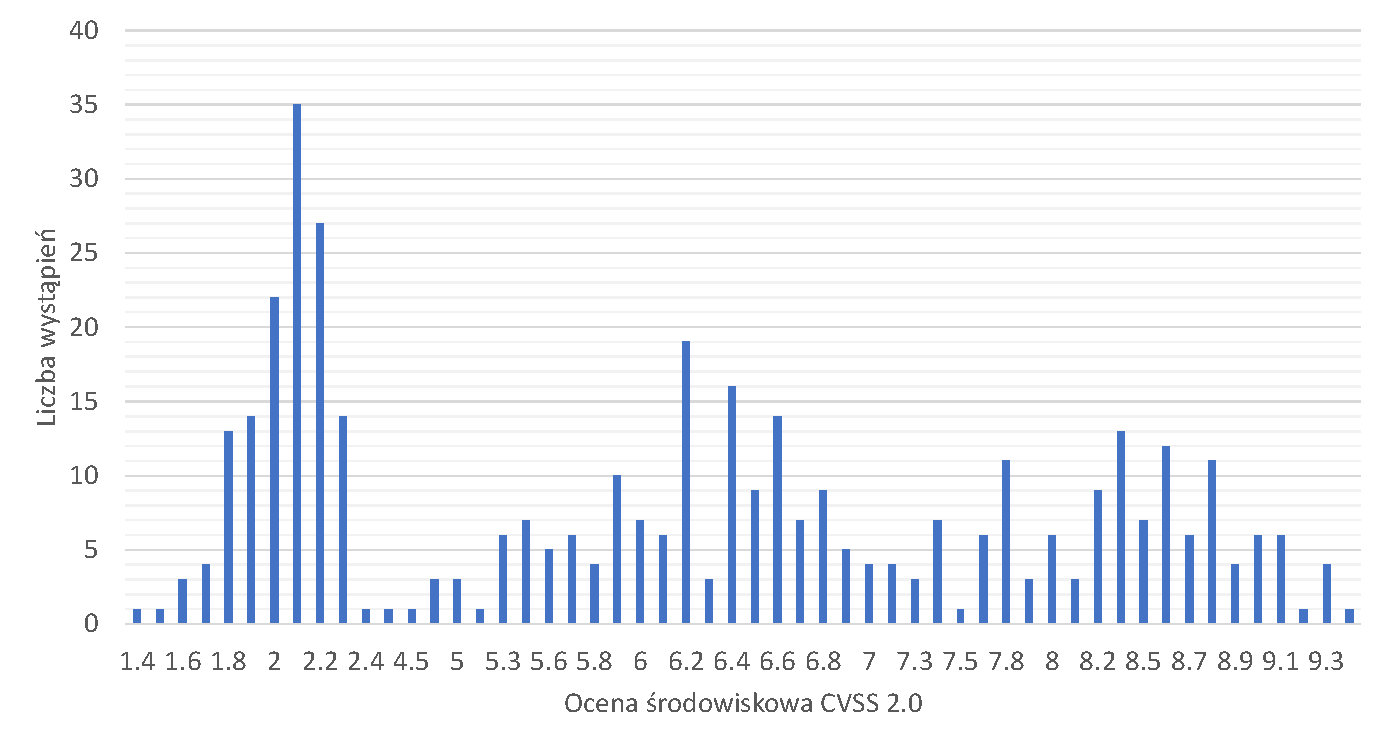
\includegraphics[width=.9\textwidth]{Chapters/Wplyw/cvss2/cvss_2_high.pdf}
\caption{Liczba wystąpień wartości oceny środowiskowej dla różnych ustawień parametrów $CIA$, $CDP$, $TD$ dla oceny bazowej CVSS 2.0 o kategorii wysokiej.}
\label{fig:wplyw:env_a:cvss_2_high}
\end{figure}

\bigbreak
Rysunek \ref{fig:wplyw:env_a:cvss_2_medium} przedstawia liczbę wystąpień wartości oceny środowiskowej dla różnych ustawień parametrów $CIA$, $CDP$, $TD$ dla oceny bazowej CVSS 2.0 o kategorii średniej. Na podstawie wyników przedstawionych na rysunku \ref{fig:wplyw:env_a:cvss_2_medium} można stwierdzić, że dla oceny bazowej CVSS 2.0 o wartości początkowej 4.3 (kategoria średnia) na 540 kombinacji parametrów $CIA$, $CDP$, $TD$ możliwe jest otrzymanie 30 unikalnych wartości oceny środowiskowej CVSS 2.0. Otrzymane wartości oceny środowiskowej CVSS 2.0 mieszczą się w zakresie od 0.8 do 7.7. Z zakresu otrzymanych wartości oceny środowiskowej CVSS 2.0 można wyciągnąć wniosek, że możliwa jest zmiana kategorii krytyczności z średniej na wysoką lub niską. Dla 540 kombinacji parametrów $CIA$, $CDP$, $TD$ dla oceny bazowej CVSS 2.0 o kategorii średniej zmiana jednego parametru środowiskowego może spowodować zmianę kategorii krytyczności na wysoką z prawdopodobieństwem 10.6\%, średnią z prawdopodobieństwem 46.9\% lub niską z prawdopodobieństwem 42.5\%.

\begin{figure}[!ht]
\centering
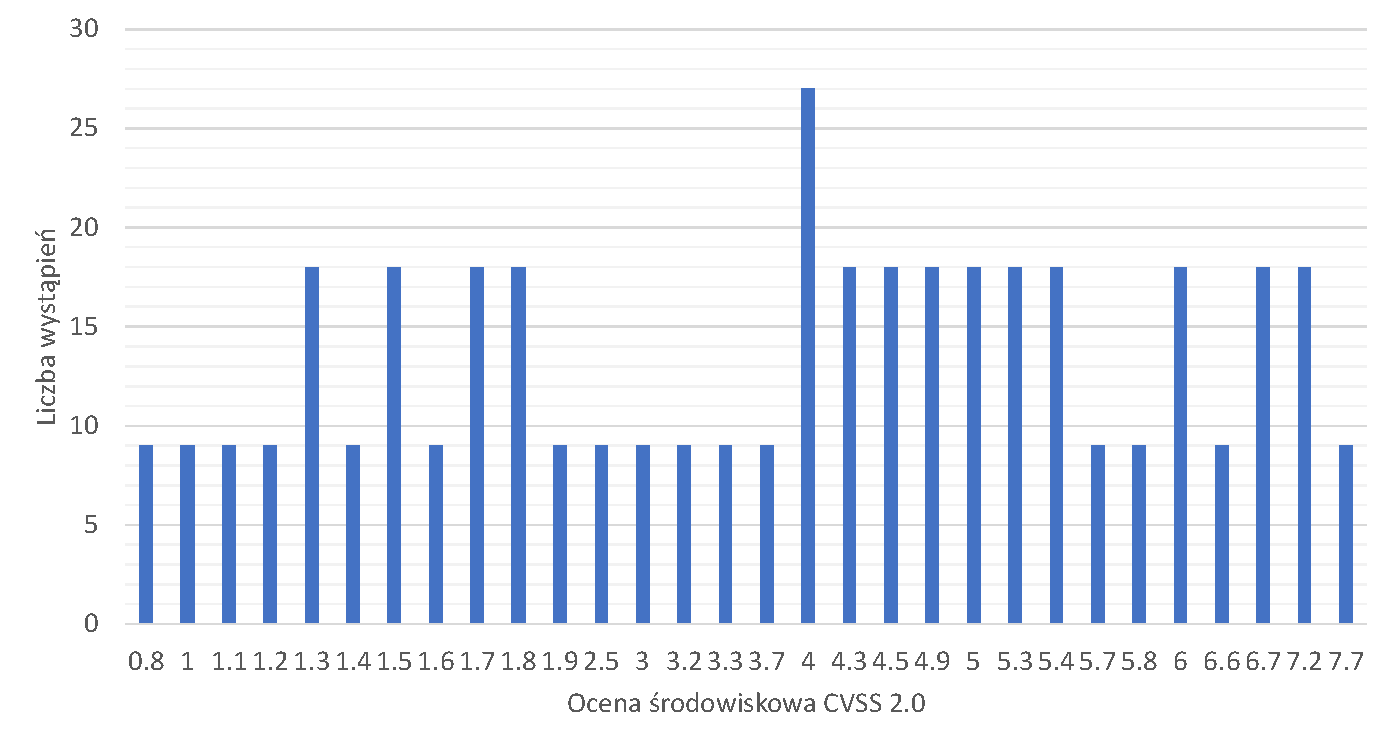
\includegraphics[width=.9\textwidth]{Chapters/Wplyw/cvss2/cvss_2_medium.pdf}
\caption{Liczba wystąpień wartości oceny środowiskowej dla różnych ustawień $CIA$, $CDP$, $TD$ dla oceny bazowej CVSS 2.0 o kategorii średniej.}
\label{fig:wplyw:env_a:cvss_2_medium}
\end{figure}

\bigbreak
Rysunek \ref{fig:wplyw:env_a:cvss_2_low} przedstawia liczbę wystąpień wartości oceny środowiskowej dla różnych ustawień parametrów $CIA$, $CDP$, $TD$ dla oceny bazowej CVSS 2.0 o kategorii niskiej. Na podstawie wyników przedstawionych na rysunku \ref{fig:wplyw:env_a:cvss_2_low} można stwierdzić, że dla oceny bazowej CVSS 2.0 o wartości początkowej 3.3 (kategoria niska) na 540 kombinacji parametrów $CIA$, $CDP$, $TD$ możliwe jest otrzymanie 47 unikalnych wartości oceny środowiskowej CVSS 2.0. Otrzymane wartości oceny środowiskowej CVSS 2.0 mieszczą się w zakresie od 0.4 do 7.4. Z zakresu otrzymanych wartości oceny środowiskowej CVSS 2.0 można wyciągnąć wniosek, że możliwa jest zmiana kategorii krytyczności z niskiej na wysoką lub średnią. Dla 540 kombinacji parametrów $CIA$, $CDP$, $TD$ dla oceny bazowej CVSS 2.0 o kategorii niskiej zmiana jednego parametru środowiskowego może spowodować zmianę kategorii krytyczności na wysoką z prawdopodobieństwem 2.2\%, średnią z prawdopodobieństwem 41.5\% lub niską z prawdopodobieństwem 56.3\%.

\begin{figure}[!ht]
\centering
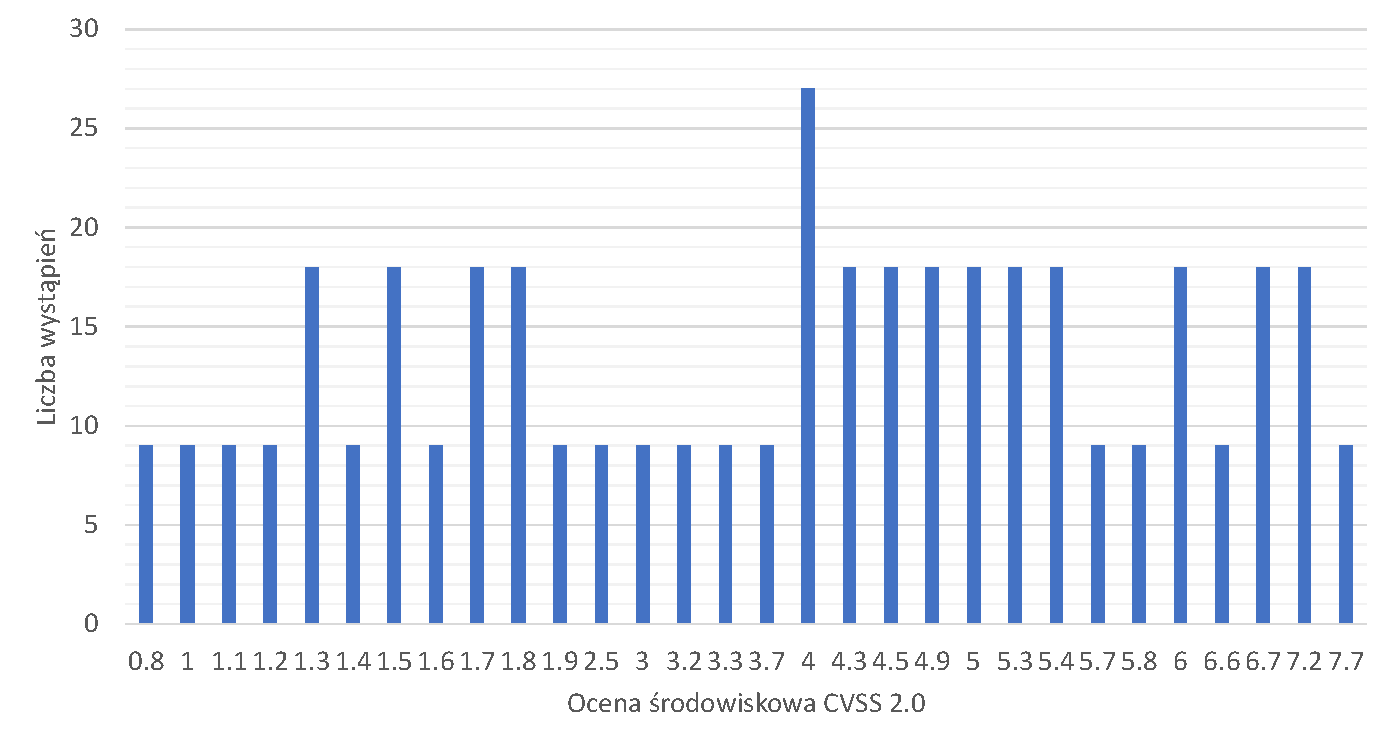
\includegraphics[width=.9\textwidth]{Chapters/Wplyw/cvss2/cvss_2_low.pdf}
\caption{Liczba wystąpień wartości oceny środowiskowej dla różnych ustawień parametrów $CIA$, $CDP$, $TD$ dla oceny bazowej CVSS 2.0 o kategorii niskiej.}
\label{fig:wplyw:env_a:cvss_2_low}
\end{figure}

\bigbreak
Na podstawie analizy wyników stwierdza się znaczący wpływ parametrów środowiskowych $TD$, $CDP$, $CIA$ na ocenę bazową CVSS 2.0. Ich prawidłowy dobór pozwala dopasować ocenę oraz krytyczność do monitorowanego środowiska teleinformatycznego dla wszystkich rozpatrywanych przypadków. Jak wykazano w analizie istnieje, 540 możliwych kombinacji parametrów środowiskowych, co przekłada się na znaczną liczbę unikalnych wartości oceny środowiskowej CVSS 2.0. Dla podatności o kategorii wysokiej z oceną bazową CVSS 2.0 o wartości 7.5 istnieje 55 unikalnych wartości oceny środowiskowej (Rysunek \ref{fig:wplyw:env_a:cvss_2_high}), która umożliwia zmianę kategorii z wysokiej na niską. Dla podatności o kategorii średniej z oceną bazową CVSS 2.0 o wartości 4.3 istnieje 30 unikalnych wartości oceny środowiskowej (Rysunek \ref{fig:wplyw:env_a:cvss_2_medium}), która umożliwia zmianę kategorii z średniej na niską lub wysoką. Dla podatności o kategorii niskiej z oceną bazową CVSS 2.0 o wartości 3.3 analiza wykazała 47 możliwych unikalnych wartości (Rysunek \ref{fig:wplyw:env_a:cvss_2_low}), która umożliwia zmianę kategorii z niskiej na średnią lub wysoką. Na podstawie otrzymanych wyników dotyczących standardu CVSS 2.0 stwierdza się, że parametry środowiskowe $CIA$, $CDP$, $TD$ mają znaczący wpływ na zmianę oceny oraz kategorii podatności. W kolejnym rozdziale przedmiotem analizy są otrzymane wyniki wybranych modeli zarządzania podatnościami wykorzystującymi standard CVSS 2.0 dla trzech niezależnych środowisk teleinformatycznych.

%%%%%%%%%%%%%%%%%%%%%%%%%%%%%%%%%%%%%%%%%%%%%%%%

%%%%%%%%%%%%%%%%%%%%%%%%%%%%%%%%%%%%%%%%%%%%%%%%
\section{Wpływ parametrów środowiskowych na ocenę bazową CVSS 3.x}
\label{sec:wplyw_cvss3}
Tabela \ref{tab:wplyw:env_a:cve_cvss_2} zawiera podatności wykryte w środowisku teleinformatycznym A dla każdej kategorii krytyczności według oceny bazowej CVSS 3.x. Podatności przedstawione w tabeli \ref{tab:wplyw:env_a:cve_cvss_2} zostały wybrane w sposób losowy w celu umożliwienia przeprowadzenia analizy wpływu parametrów $CIA$ na zmianę kategorii krytyczności. W przypadku zastosowania parametrów $CIA$ istnieją 64 możliwe kombinacje parametrów środowiskowych $CIA$. Natomiast według dokumentacji \cite{cvs2019specification} można wykluczyć wartości \emph{Not Defined} (X), ponieważ nie mają one wpływu na ocenę bazową. W związku z czym pozostaje tylko 27 możliwych kombinacji.

\begin{table}[tbh]
\caption{Podatności wykryte w środowisku teleinformatycznym A dla każdej kategorii krytyczności według oceny bazowej CVSS 3.x.}
\begin{center}
\label{tab:wplyw:env_a:cve_cvss_3}
\begin{tabular}{lcl}
\hline \noalign {\smallskip}
\textbf{CVE ID}  & \textbf{Ocena bazowa} & \textbf{Kategoria}  \\
                 & \textbf{CVSS 3.x} &  \\
\hline \noalign {\smallskip}
CVE-2019-13224 & 9.8 & Krytyczna \\
CVE-2020-7062  & 7.5 & Wysoka \\
CVE-2020-7066  & 4.3 & Średnia \\
CVE-2020-7068  & 3.6 & Niska \\
\hline \noalign {\smallskip}
\end{tabular}
\end{center}
\end{table}

\begin{comment}
\bigbreak
Rysunek \ref{fig:wplyw:env_a:cvss_3_distribution} przedstawia wpływ ustawień parametrów środowiskowych $CIA$ na oceny bazowe CVSS 3.x dla podatności wskazanych w tabeli \ref{tab:wplyw:env_a:cve_cvss_3}. Na podstawie wyników przedstawionych na rysunku \ref{fig:wplyw:env_a:cvss_3_distribution} można stwierdzić, że liczba możliwych wartości oceny środowiskowej CVSS 3.x jest bardzo ograniczona w porównaniu do oceny środowiskowej CVSS 2.0. Natomiast nie zmienia to faktu, że każda z przedstawionych podatności za pomocą parametrów $CIA$ może zmienić kategorię krytyczności co zostało potwierdzone w dalszej części analizy.

\begin{figure}[!ht]
\centering
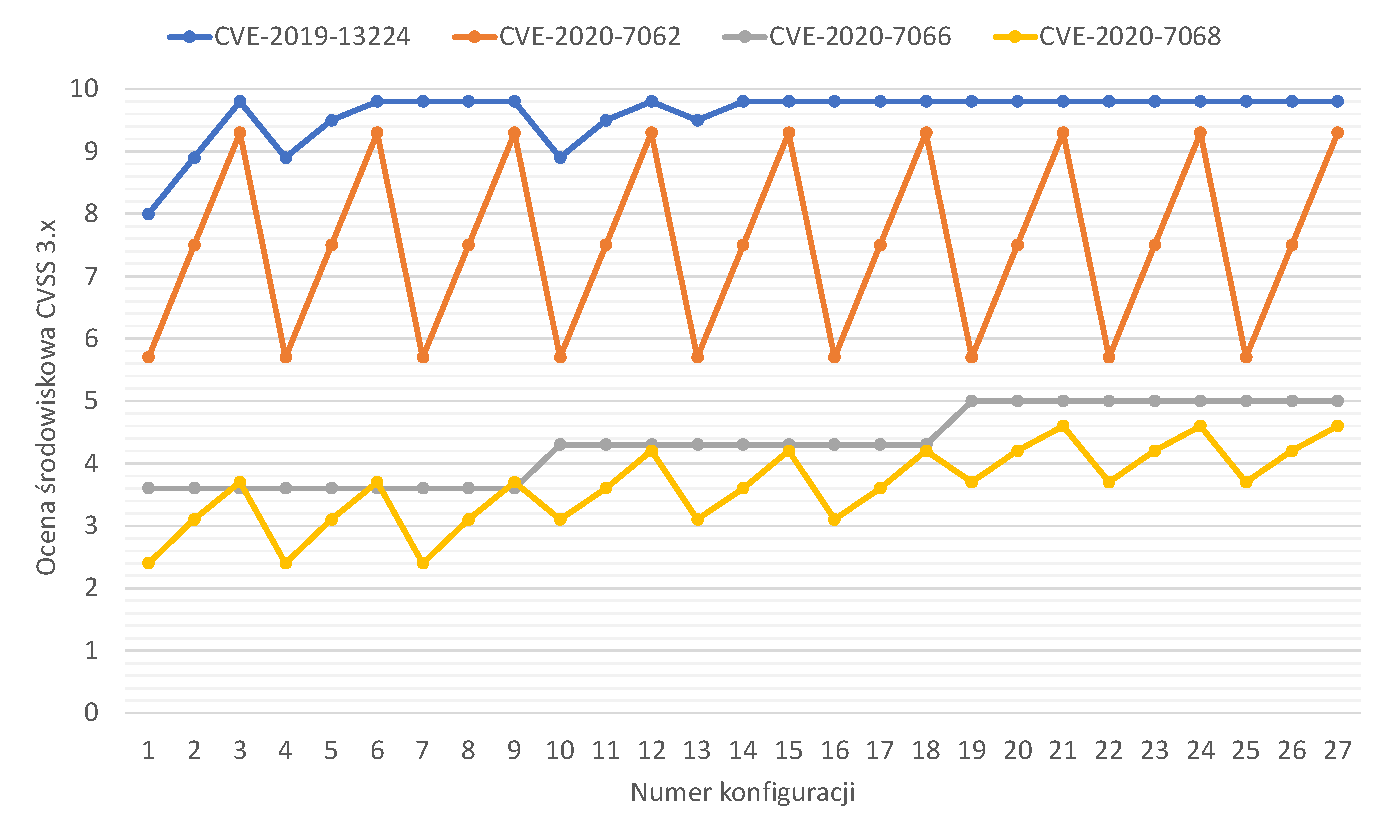
\includegraphics[width=.9\textwidth]{Chapters/Wplyw/cvss3/cvss_3_distribution.pdf}
\caption{Wpływ ustawień parametrów środowiskowych $CIA$ na oceny bazowe CVSS 3.x dla podatności wskazanych w tabeli \ref{tab:wplyw:env_a:cve_cvss_3}.}
\label{fig:wplyw:env_a:cvss_3_distribution}
\end{figure}
\end{comment}

\bigbreak
Rysunek \ref{fig:wplyw:env_a:cvss_3_critical} przedstawia liczbę wystąpień wartości oceny środowiskowej dla różnych ustawień parametrów $CIA$ dla oceny bazowej CVSS 3.x o kategorii krytycznej. Na podstawie wyników przedstawionych na rysunku \ref{fig:wplyw:env_a:cvss_3_critical} można stwierdzić, że dla oceny bazowej CVSS 3.x o wartości początkowej 9.8 (kategoria krytyczna) na 27 kombinacji parametrów $CIA$ otrzymano 4 unikalne wartości oceny środowiskowej CVSS 3.x. Otrzymane wartości oceny środowiskowej CVSS 3.x mieszczą się w zakresie od 8 do 9.8. Z zakresu otrzymanych wartości oceny środowiskowej CVSS 3.x można stwierdzić, że możliwa jest zmiana kategorii z krytyczej na wysoką. Dla 27 kombinacji parametrów $CIA$ dla oceny bazowej CVSS 3.x o kategorii krytycznej zmiana jednego parametru środowiskowego może spowodować zmianę kategorii krytyczności na wysoką z prawdopodobieństwem 3.7\% lub krytyczną z prawdopodobieństwem 96.3\%.

\begin{figure}[!ht]
\centering
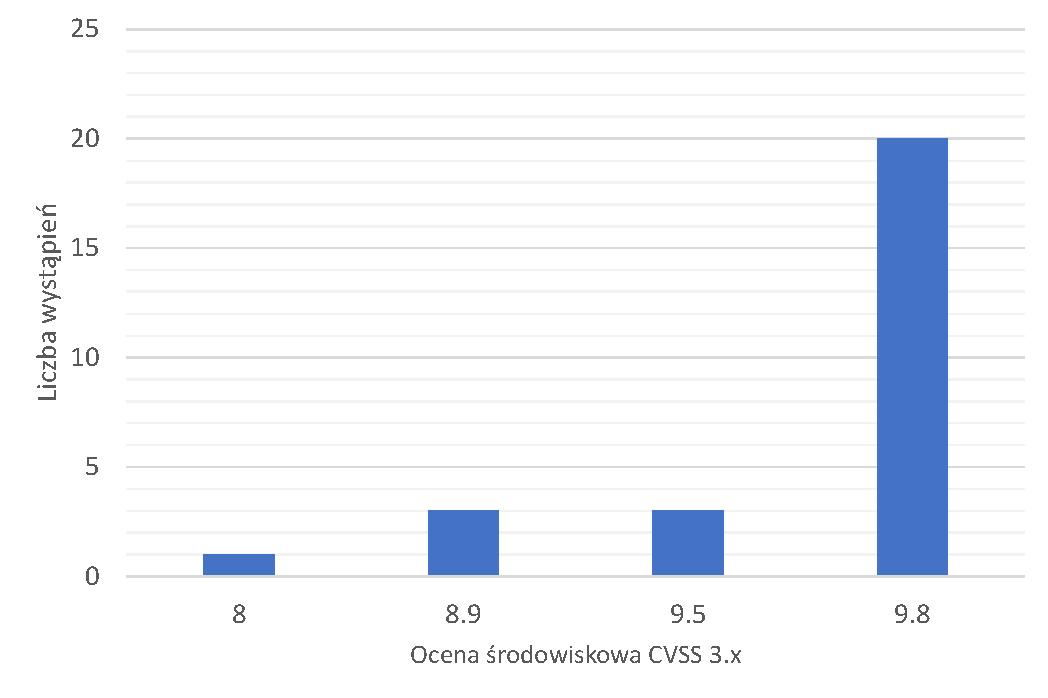
\includegraphics[width=.9\textwidth]{Chapters/Wplyw/cvss3/cvss_3_critical.pdf}
\caption{Liczba wystąpień wartości oceny środowiskowej dla różnych ustawień parametrów $CIA$ dla oceny bazowej CVSS 3.x o kategorii krytycznej.}
\label{fig:wplyw:env_a:cvss_3_critical}
\end{figure}

\bigbreak
Rysunek \ref{fig:wplyw:env_a:cvss_3_high} przedstawia liczbę wystąpień wartości oceny środowiskowej dla różnych ustawień parametrów $CIA$ dla oceny bazowej CVSS 3.x o kategorii wysokiej. Na podstawie wyników przedstawionych na rysunku \ref{fig:wplyw:env_a:cvss_3_high} można stwierdzić, że dla oceny bazowej CVSS 3.x o wartości początkowej 7.5 (kategoria wysoka) na 27 kombinacji parametrów $CIA$ otrzymano tylko 3 unikalne wartości oceny środowiskowej CVSS 3.x. Otrzymane wartości oceny środowiskowej CVSS 3.x mieszczą się w zakresie od 5.7 do 9.3. Z zakresu otrzymanych wartości oceny środowiskowej CVSS 3.x można stwierdzić, że możliwa jest zmiana kategorii z wysokiej na średnią lub krytyczną. Dla 27 kombinacji parametrów $CIA$ dla oceny bazowej CVSS 3.x o kategorii wysokiej zmiana jednego parametru środowiskowego może spowodować zmianę kategorii krytyczności na krytyczną z prawdopodobieństwem 33.(3)\%, średnią z prawdopodobieństwem 33.(3)\% lub wysoką z prawdopodobieństwem 33.(3)\%.

\begin{figure}[!ht]
\centering
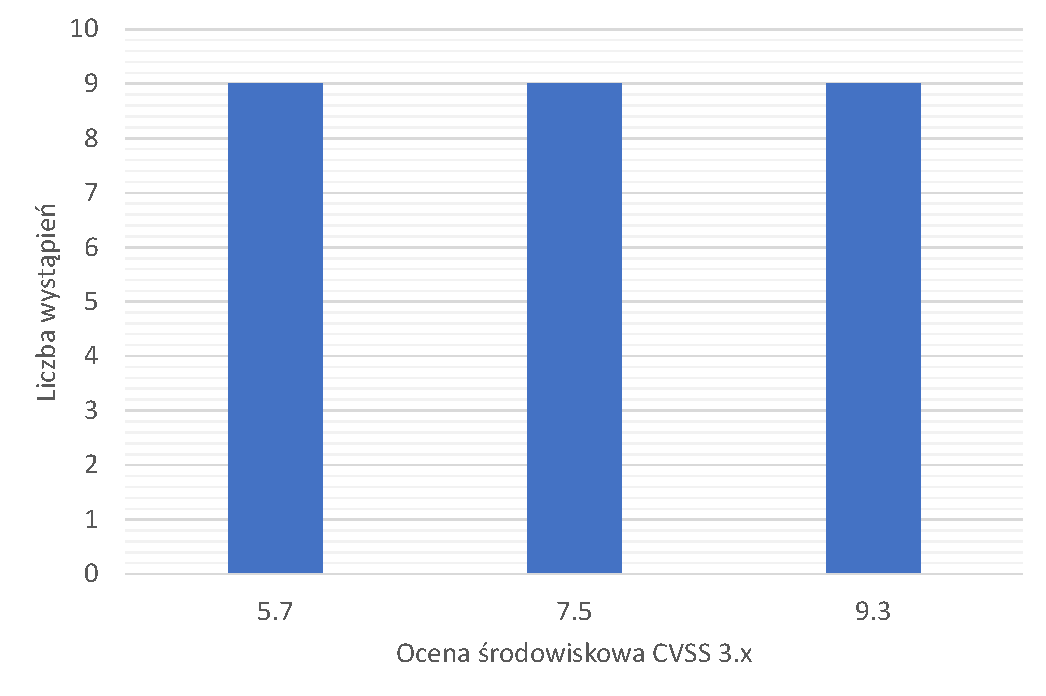
\includegraphics[width=.9\textwidth]{Chapters/Wplyw/cvss3/cvss_3_high.pdf}
\caption{Liczba wystąpień wartości oceny środowiskowej dla różnych ustawień parametrów $CIA$ dla oceny bazowej CVSS 3.x o kategorii wysokiej.}
\label{fig:wplyw:env_a:cvss_3_high}
\end{figure}

\bigbreak
Rysunek \ref{fig:wplyw:env_a:cvss_3_medium} przedstawia liczbę wystąpień wartości oceny środowiskowej dla różnych ustawień parametrów $CIA$ dla oceny bazowej CVSS 3.x o kategorii średniej. Na podstawie wyników przedstawionych na rysunku \ref{fig:wplyw:env_a:cvss_3_medium} można stwierdzić, że dla oceny bazowej CVSS 3.x o wartości początkowej 4.3 (kategoria średnia) na 27 kombinacji parametrów $CIA$ otrzymano tylko 3 unikalne wartości oceny środowiskowej CVSS 3.x. Otrzymane wartości oceny środowiskowej CVSS 3.x mieszczą się w zakresie od 3.6 do 5.0. Z zakresu otrzymanych wartości oceny środowiskowej CVSS 3.x można stwierdzić, że możliwa jest zmiana kategorii z średniej na niską. Dla 27 kombinacji parametrów $CIA$ dla oceny bazowej CVSS 3.x o kategorii wysokiej, zmiana jednego parametru środowiskowego może spowodować zmianę kategorii krytyczności na średnią z prawdopodobieństwem 66.(6)\% lub niską z prawdopodobieństwem 33.(3)\%.

\begin{figure}[!ht]
\centering
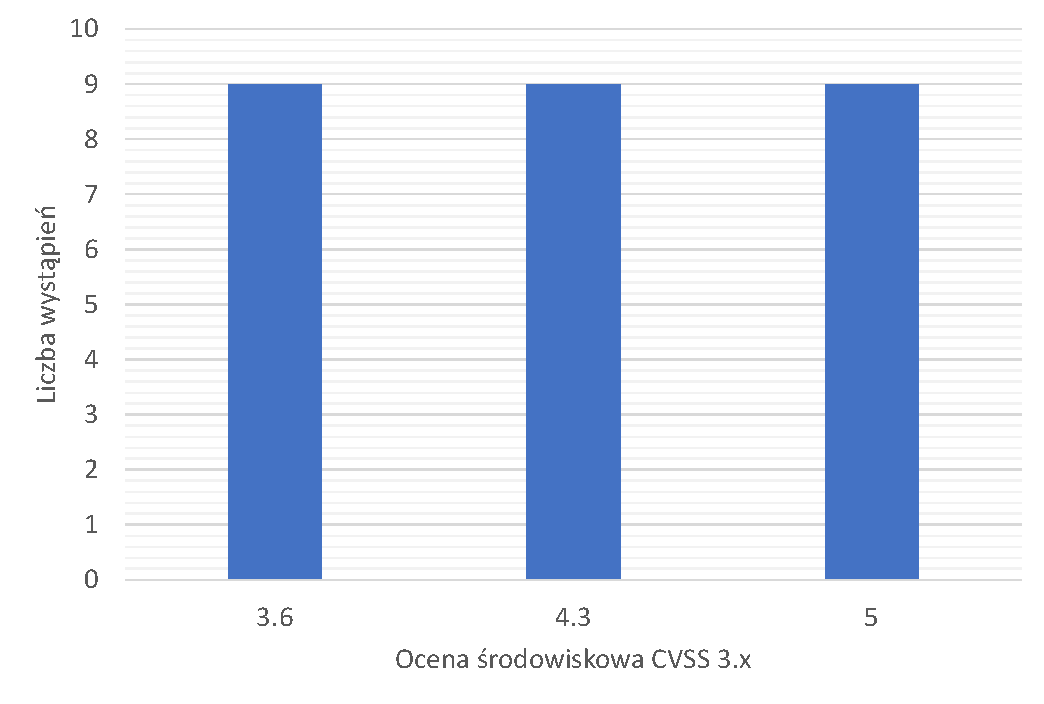
\includegraphics[width=.9\textwidth]{Chapters/Wplyw/cvss3/cvss_3_medium.pdf}
\caption{Liczba wystąpień wartości oceny środowiskowej dla różnych ustawień parametrów $CIA$ dla oceny bazowej CVSS 3.x o kategorii średniej.}
\label{fig:wplyw:env_a:cvss_3_medium}
\end{figure}

\bigbreak
Rysunek \ref{fig:wplyw:env_a:cvss_3_low} przedstawia liczbę wystąpień wartości oceny środowiskowej dla różnych ustawień parametrów $CIA$ dla oceny bazowej CVSS 3.x o kategorii niskiej. Na podstawie wyników przedstawionych na rysunku \ref{fig:wplyw:env_a:cvss_3_low} można stwierdzić, że dla oceny bazowej CVSS 3.x o wartości początkowej 3.6 (kategoria niska) na 27 kombinacji parametrów $CIA$ otrzymano 6 unikalnych wartości oceny środowiskowej CVSS 3.x. Otrzymane wartości oceny środowiskowej CVSS 3.x mieszczą się w zakresie od 2.4 do 4.6. Z zakresu otrzymanych wartości oceny środowiskowej CVSS 3.x można stwierdzić, że możliwa jest zmiana kategorii z niskiej na średnią. Dla 27 kombinacji parametrów $CIA$ dla oceny bazowej CVSS 3.x o kategorii niskiej zmiana jednego parametru środowiskowego może spowodować zmianę kategorii krytyczności na niską z prawdopodobieństwem 66.(6)\% lub średnią z prawdopodobieństwem 33.(3)\%.

\begin{figure}[!ht]
\centering
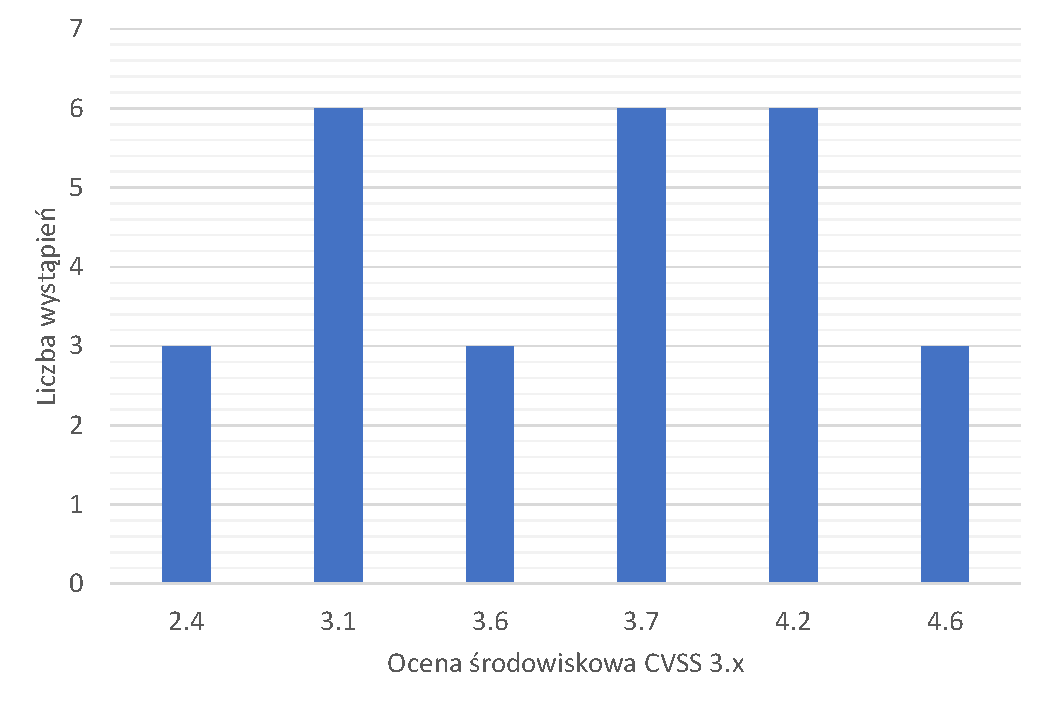
\includegraphics[width=.9\textwidth]{Chapters/Wplyw/cvss3/cvss_3_low.pdf}
\caption{Liczba wystąpień wartości oceny środowiskowej dla różnych ustawień parametrów $CIA$ dla oceny bazowej CVSS 3.x o kategorii niskiej.}
\label{fig:wplyw:env_a:cvss_3_low}
\end{figure}

\bigbreak
Na podstawie analizy wyników stwierdza się znaczący wpływ parametrów środowiskowych $CIA$ na ocenę bazową CVSS 3.x. Otrzymane wyniki potwierdzają, że prawidłowy dobór parametrów środowiskowych $CIA$ pozwala dopasować ocenę oraz kategorię do monitorowanego środowiska teleinformatycznego. Jak wykazano w analizie, istnieje 27 możliwych kombinacji wartości parametrów środowiskowych $CIA$, które mogą zmieniać kategorię krytyczności podatności. Dla podatności o kategorii wysokiej z oceną bazową CVSS 3.x wynoszącą 9.8 istnieją 4 możliwe unikalne wartości oceny środowiskowej (Rysunek \ref{fig:wplyw:env_a:cvss_3_critical}), które umożliwiają zmianę kategorii tylko z krytycznej na wysoką. Dla podatności o kategorii wysokiej z oceną bazową CVSS 3.x wynoszącą 7.5, istnieją tylko 3 możliwe unikalne wartości oceny środowiskowej, które umożliwiają zmianę kategorii z wysokiej na średnią lub krytyczną. Dla podatności o kategorii średniej z oceną bazową CVSS 3.x wynoszącą 4.3 istnieją 3 możliwe unikalne wartości oceny środowiskowej, które pozwalają na zmianę kategorii krytyczności z średniej na niską. Dla podatności o kategorii niskiej z oceną bazową CVSS 3.x wynoszącą 3.6 istnieje 6 możliwych unikalnych wartości oceny środowiskowej, dzięki którym możliwa jest zmiana kategorii z niskiej na średnią. Na podstawie otrzymanych wyników dotyczących standardu CVSS 3.x stwierdza się, że parametry środowiskowe $CIA$ mają znaczący wpływ na zmianę oceny oraz kategorii podatności. W kolejnym rozdziale przedmiotem analizy są otrzymane wyniki wybranych modeli zarządzania podatnościami wykorzystującymi standard CVSS 3.x dla trzech niezależnych środowisk teleinformatycznych.

%%%%%%%%%%%%%%%%%%%%%%%%%%%%%%%%%%%%%%%%%%%%%%%%

%%%%%%%%%%%%%%%%%%%%%%%%%%%%%%%%%%%%%%%%%%%%%%%%
\section{Wyniki analizy metod konwersji oceny bazowej CVSS 2.0 do 3.x}
\label{sec:ml_analiza}

Tabela \ref{tab2} przedstawia wybrane algorytmy klasyfikacji z uwzględnieniem liczby PC i liczby elementów wektora uczącego do określenia parametrów oceny bazowej CVSS 3.x.
Tabela \ref{tab2} zawiera informacje, przy której wartości PC  i dla jakiej liczby dodatkowych elementów wektora oceny bazowej CVSS 2.0 uzyskano wysoką i powtarzalną wartość skuteczności klasyfikacji. Dla parametrów opisanych w tabeli \ref{tab2}, zbiór uczący składał się z 1 968 wektorów.


\begin{table}[htbp]
\caption{Wybrane algorytmy klasyfikacji, z uwzględnieniem liczby PC i liczby elementów wektora uczącego do określenia parametrów oceny bazowej CVSS 3.x.}
\begin{center}
\begin{tabular}{cccc}
\hline
\textbf{Parametr oceny} & \textbf{Algorytm}   & \textbf{Liczba}  & \textbf{Liczba elementów}  \\
\textbf{bazowej CVSS 3.x}  &             & \textbf{PC}    & \textbf{wektora}    \\
\hline
AV           & KSVM(TGRBF)    & 35     & 100   \\
AC           & PNN            & 25     & 100   \\
PR           & KSVM(TGRBF)    & 24     & 50    \\
U            & PNN            & 41     & 100   \\
C            & KSVM(TGRBF)    & 43     & 50    \\
I            & KSVM(TGRBF)    & 32     & 100   \\
A            & PNN            & 48     & 100   \\
S            & NB             & 38     & 100   \\
\hline
\end{tabular}
\label{tab2}
\end{center}
\end{table}

\bigbreak
Rysunek \ref{fig:wplyw:ml:fig_1} przedstawia średnią dokładność klasyfikacji parametrów wektora oceny bazowej CVSS 3.x za pomocą algorytmów przedstawionych w tabeli \ref{tab2}. Wyniki ukazane na rysunku \ref{fig:wplyw:ml:fig_1} zostały obliczone na podstawie wykonania dziesięciu prób testowych na 71 000 losowo wybranych wektorach. Dokładność obliczono, sumując liczbę poprawnych klasyfikacji i dzieląc przez liczbę wszystkich wektorów testujących. Wyniki przedstawione na rysunku \ref{fig:wplyw:ml:fig_1} pokazują, że dla wszystkich parametrów mediana skuteczności klasyfikacji przekracza 90\%. Uzyskane wyniki są bardzo powtarzalne, poza parametrami AV i PR. W przypadku AV rozpiętości są większe, ale minimalna wartość dokładności wynosi 88,2\%. Prawidłowa klasyfikacja AV z wersji oceny bazowej CVSS 2.0 do 3.x jest utrudniona ze względu na różnicę w standardach CVSS. W przypadku klasyfikacji PR wystąpiły 2 wartości odstające, z wartością minimalną 87,81 \%. Przy obliczaniu zakresu najlepszy okazuje się algorytm NB (mediana to 94,86\%). Bardziej zaawansowane metody są o kilka punktów procentowych gorsze. Parametry AC, U i A były bardzo dobrze konwertowane przez PNN, która dodatkowo należy do algorytmów szybkiego uczenia. W najtrudniejszych przypadkach – AV, PR, C i I najlepszą skuteczność rozpoznawania zapewnia SVM TGRBF. Stopień złożoności tego algorytmu przekłada się na wydłużony czas przetwarzania w porównaniu z innymi algorytmami.

\begin{figure}[!ht]
\centering
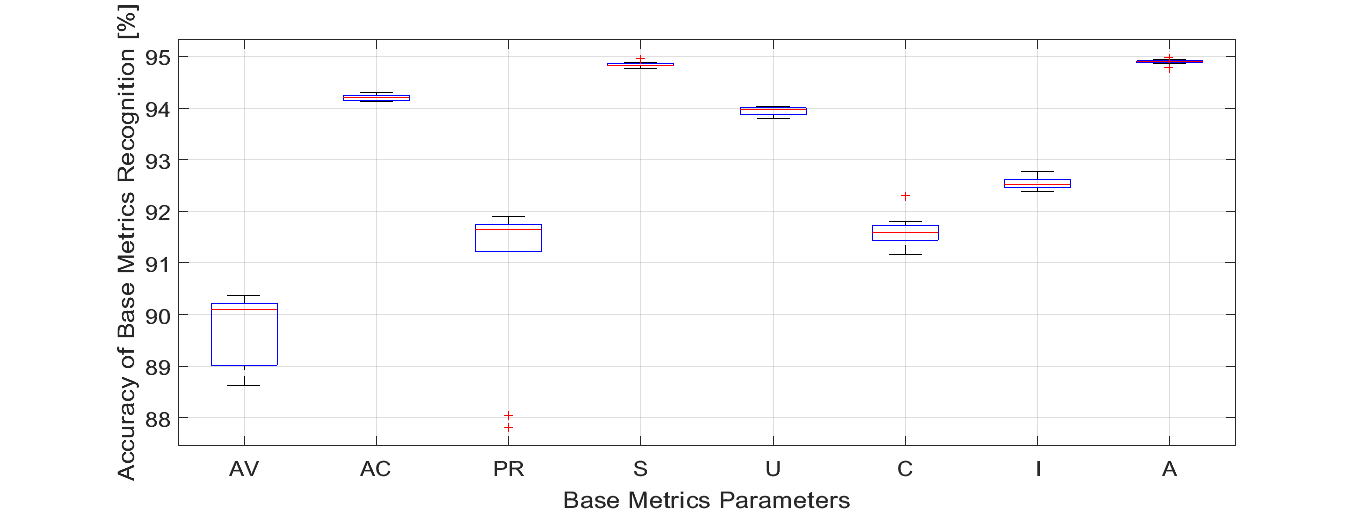
\includegraphics[width=0.95\textwidth]{Chapters/Wplyw/ml_results/Param_Limit_71000_multi_10.png}
\caption{Statystyka dokładność klasyfikacji parametrów wektora oceny bazowej CVSS 3.x za pomocą programu algorytmów przedstawionych tabeli \ref{tab2}.}
\label{fig:wplyw:ml:fig_1}
\end{figure}

\bigbreak
Tabela \ref{tab3} przedstawia medianę i średnią dokładność obliczoną dla algorytmów przedstawionych w tabeli \ref{tab2}. Wyniki przedstawione w tabeli \ref{tab3} zostały uzyskane z 10 krotnej próby testowej algorytmów z losowo wybranym 71 000 zbiorem testowym. Na podstawie wyników przedstawionych w tabeli \ref{tab3} można stwierdzić, że poza AV i PR wykazują niewielkie odchylenie standardowe od średniej, a wartości średnie różnią się od mediany maksymalnie o 0,07\%. Otrzymane wyniki potwierdzają wysoką precyzję określania parametrów oceny bazowej CVSS 3.x przez wybrane algorytmy.

\begin{table}[htbp]
\caption{Mediana i średnia dokładność obliczona dla algorytmów przedstawionych w tabeli \ref{tab2}.}
\begin{center}
\begin{tabular}{cccc}
\hline
\textbf{Parametr oceny} & \textbf{Mediana [\%]}   & \textbf{Średnia [\%]}  \\
\textbf{bazowej CVSS 3.x} & & \\
\hline
AV           & 90.10    & $89.73\pm0.66$     \\
AC           & 94.21    & $94.21\pm0.06$     \\
PR           & 91.64    & $90.89\pm1.49$     \\
S            & 94.86    & $94.84\pm0.05$     \\
U            & 94.02    & $93.95\pm0.07$     \\
C            & 91.59    & $91.62\pm0.29$     \\
I            & 92.51    & $92.53\pm0.11$     \\
A            & 94.94    & $94.90\pm0.05$     \\
\hline
\end{tabular}
\label{tab3}
\end{center}
\end{table}

\bigbreak
Rysunek \ref{fig:wplyw:ml:qsrs_base_score} przedstawia macierz błędów klasyfikacji kategorii podatności z oceny bazowej CVSS 2.0 do 3.x. Wyniki przedstawione na rysunku \ref{fig:wplyw:ml:qsrs_base_score} zostały uzyskane dla 71 000 podatności pobranych z serwisu NVD \cite{booth2013national}. Na rysunku \ref{fig:wplyw:ml:qsrs_base_score} klasa 0 oznacza podatność o klasyfikacji informacyjnej; 1 - niskiej; 2 - średniej; 3 - wysokiej; oraz 4 - krytycznej. Na podstawie wyników przedstawionych na rysunku \ref{fig:wplyw:ml:qsrs_base_score} można stwierdzić, że zastosowane rozwiązanie najlepiej radzi sobie z klasyfikacją oceny bazowej CVSS 3.x dla kategorii krytycznej (precyzja 90.3\%, czułość 87.8\%), a najgorzej z klasyfikacją dla kategorii niskiej (precyzja 27\%, czułość 12.4\%). Dodatkowo na podstawie wyników przedstawionych na rysunku \ref{fig:wplyw:ml:qsrs_base_score} można stwierdzić, że średnia sprawność dla klasyfikacji wszystkich kategorii wynosi 86\%.

\begin{figure}[!ht]
\centering
\includegraphics[width=0.95\textwidth]{Chapters/Wplyw/ml_results/Macierz_błędów_QSRS.png}
\caption{Macierz błędów klasyfikacji kategorii podatności z oceny bazowej CVSS 2.0 do 3.x.}
\label{fig:wplyw:ml:qsrs_base_score}
\end{figure}

\bigbreak
Na podstawie uzyskanych wyników stwierdza się, że zaproponowane algorytmy uczenia maszynowego wykorzystane do konwersji oceny bazowej CVSS 2.0 do 3.x wykazują wysoką skuteczność wyznaczania podstawowych parametrów wektora oceny bazowej CVSS 3.x. Otrzymana mediana dla najgorszego rozpatrywanego przypadku, tj. dla parametru AV, przekracza 90\%. Na podstawie otrzymanych wyników można stwierdzić, że sprawność obliczania oceny bazowej CVSS 3.x wynosi 62.8\%, natomiast średnia sprawność klasyfikacji dla wszystkich kategorii krytyczności wynosi 86\%.


\chapter{Analiza}
Przedmiotem rozważań w rozdziale 5 są wyniki analizy wybranych modeli zarządzania podatnościami otrzymane dla trzech niezależnych środowisk teleinformatycznych. Środowiska teleinformatyczne omówione szczegółowo w rozdziale 3 są zróżnicowane aby ułatwić omówienie wad i zalet analizowanych modeli zarządzania podatnościami, które zaproponowano w rozdziale 1. Nie oznacza to jednak, że zaproponowane w rozdziale 2 rozwiązania mogą być wykorzystane tylko i wyłącznie w analizowanych środowiskach teleinformatycznych. Na podstawie otrzymanych wyników można bowiem wyciągnąć wnioski o charterze ogólnym stosowalne dla dowolnego środowiska teleinformatycznego. Wybrane środowiska teleinformatyczne różnią się liczbą wykrytych podatności, a także liczbą podatności, dla których znana jest ocena bazowa dla standardu CVSS 2.0 oraz 3.x. Dodatkowa różnica pomiędzy środowiskami teleinformatycznymi odnosi się do informacji otrzymanych od administratorów. Dla środowiska teleinformatycznego A, oprócz podania danych na temat wykrytych podatności, administrator przekazał informacje dotyczące ustawień parametrów środowiskowych $CIA$. Dla środowiska teleinformatycznego B otrzymano tylko raport z wykrytymi podatnościami za pomocą oprogramowania Nessus. Dla środowiska teleinformatycznego C otrzymano raport z podatnościami wykrytymi za pomocą oprogramowania Nessus oraz ogólne informacje dotyczące wag skanowanych zasobów. Wyniki otrzymane dla tychże trzech różnych i niezależnych środowisk teleinformatycznych wykorzystano w tym rozdziale do analizy modeli procesu zarządzania podatnościami (Rozdział \ref{sec:modele-zarzadzaia-podatnosciami}). 

\bigbreak
Dla każdego rozpatrywanego środowiska wyniki analizy uporządkowano w następujący sposób. Najpierw porównano modele zarządzania podatnościami, które wykorzystują standard CVSS 2.0 (Rysunek \ref{fig:chapter1:vm-model-cvss2}, \ref{fig:chapter1:vm-model-cvss2e}). W tym celu do oceny bazowej CVSS 2.0 dodano dane środowiskowe, a następnie przeanalizowano liczbę oraz zakres zmian w kategoriach podatności w porównaniu z oceną bazowa CVSS 2.0. Jak wykazano w tym rozdziale w oparciu o przeprowadzoną analizę, model zarządzania podatnościami, który wykorzystuje ocenę środowiskową CVSS 2.0 ma istotną wadę. Wada ta polega na tym, że parametr $TD$, który służy do ustalania liczby systemów wrażliwych na daną podatność, znacząco zaniża oceny wszystkich wykrytych podatności. Dlatego też ocena środowiskowa CVSS 2.0 nie jest dokładną miarą bezpieczeństwa infrastruktury teleinformatycznej. Konieczne było zatem rozważenie modelu zarządzania podatnościami, który opiera się na standardzie CVSS 3.x. Dokonano więc analizy modelu zarządzania podatnościami, która oprócz oceny bazowej CVSS 3.x uwzględnia także dane środowiskowe. Następnie ponownie przeanalizowano liczbę oraz zakres zmian w kategoriach podatności dla takiego modelu zarządzania podatnościami. Należy jednak zauważyć, ze implementacja modelu zarządzania podatnościami, które wykorzystuje standard CVSS 3.x okazała się trudna w praktyce. Jest bowiem wiele podatności, dla których znana jest tylko ocena bazowa CVSS 2.0. Wykonanie priorytetyzacji za pomocą modeli zarządzania podatnościami według standardu CVSS 3.x (Rysunek \ref{fig:chapter1:vm-model-cvss3}, \ref{fig:chapter1:vm-model-cvss3e}) nie było zatem w pełni możliwe z powodu braku ocen bazowych CVSS 3.x dla niektórych z wykrytych podatności. Problem ten rozwiązano przez zastosowanie metod uczenia maszynowego, które wykorzystano do przeprowadzenia konwersji oceny bazowej ze standardu CVSS 2.0 do standard 3.x, w przypadku podatności, dla których znana jest jedynie ocena bazowa CVSS 2.0. Szczegóły tej konwersji są opisane w w rozdziale \ref{sec:ml}. Po przeprowadzeniu konwersji możliwa była pełna implementacja modelu zarządzania podatnościami dla standardu 3.x i oszacowanie liczby oraz zakresu zmian w poszczególnych kategoriach podatności. Ponadto dla każdego środowiska teleinformatycznego oraz analizowanego modelu zarządzania podatnościami oszacowano liczbę roboczogodzin wymaganych do usunięcia wszystkich podatności z wyjątkiem podatności o krytyczności niskiej. W tym celu skorzystano z równań wyprowadzonych w rozdziale \ref{sec:modele-ewaluacji-efektywnosci}. Otrzymane wyniki pozwoliły na wyciągnięcie istotnych wniosków dotyczących wpływu danych środowiskowych na ocenę bazową CVSS.

\bigbreak
W rozdziale 5 przeprowadzono także analizę skalowalności opracowanego oprogramowania. Czas oczekiwania na wyniki priorytetyzacji podatności jest niezwykle istotny, ponieważ jest to również czas ekspozycji środowiska teleinformatycznego na zagrożenia wynikające z możliwości wykorzystania danej podatności przez atakującego. Redukcja czasu oczekiwania na wyniki priorytetyzacji podatności jest istotna także dlatego, że wykrywane jest coraz więcej podatności, ponadto środowiska teleinformatyczne mogą podlegać szybkim zmianom. Czas reakcji jest zatem krytycznym parametrem, gdy rozważa się bezpieczeństwo zasobów systemu teleinformatycznego. Dlatego też w ramach przeprowadzonych badań oszacowano czas trwania obliczeń w zależności od liczby modułów obliczeniowych oraz liczby przetwarzanych danych. Analiza ta została przeprowadzona w środowisku opisanym w rozdziale \ref{sec:desc_skalowalnosc}, ponieważ właściciele zasobów udostępniających dane dotyczące wykrytych podatności nie wyrazili zgody na przetwarzanie danych w chmurze.

\bigbreak
Rozdział 5 składa się z trzech części. W pierwszej części omówione zostały wyniki analizy skalowalności opracowanego rozwiązania w środowisku chmurowym. W części drugiej, omówione zostały wyniki analizy otrzymane dla środowisk teleinformatycznych przedstawionych w rozdziałach \ref{sec:desc_a}, \ref{sec:desc_b}, \ref{sec:desc_c}. Część trzecia poświęcona jest podsumowaniu uzyskanych wyników.

%%%%%%%%%%%%%%%%%%%%%%%%%%%%%%%%%%%%%%%%%%%%%%%%

%%%%%%%%%%%%%%%%%%%%%%%%%%%%%%%%%%%%%%%%%%%%%%%%
\section{Analiza czasu obliczeń obliczeń dla dużej ilości danych}
\label{sec:analiza_skalowania}
Właściciele zasobów, od których pozyskano informacje na temat podatności znajdujących się w ich infrastrukturze (Rozdziały \ref{sec:desc_a}, \ref{sec:desc_b}, \ref{sec:desc_c}) nie wyrazili zgody na przetwarzanie danych w chmurze. Dlatego w celu przeprowadzenia analizy, skalowalności rozwiązania oraz pomiaru czasu wykonywania obliczeń stworzono środowisko wirtualne zawierające 2 110 adresy IP. Dla każdego adresu IP przydzielono w sposób losowy podatności z publicznie dostępniej bazy podatności NVD \cite{booth2013national}. W rezultacie otrzymano wirtualne środowisko zawierające 168 940 podatności, z czego 3 008 podatności było unikalnych, to znaczy, że wystąpiło tylko raz na jednym adresie IP. Następnie przygotowano środowisko chmurowe, które wykorzystuje konfiguracje opisaną w rozdziale \ref{sec:desc_skalowalnosc} oraz przygotowano 12 scenariuszy testowych $P_0$ - $P_{12}$, dla których zmierzono czas trwania obliczeń:
\begin{description}
    \item $P_0$ — obliczenie oceny środowiskowej CVSS 2.0 i CVSS 3.x dla stworzonego środowiska wirtualnego,
    \item $P_1$ — obliczenie oceny środowiskowej CVSS 2.0 i CVSS 3.x dla stworzonego środowiska wirtualnego, przy czym dla 10\% zasobów (adresów IP) zmieniono składową środowiskową wektora CVSS (jeden z parametrów $CIA$),
    \item $P_2$ — obliczenie oceny środowiskowej CVSS 2.0 i CVSS 3.x dla stworzonego środowiska wirtualnego, przy czym dla 20\% zasobów (adresów IP) zmieniono składową środowiskową wektora CVSS (jeden z parametrów $CIA$),
    \item $P_3$ — obliczenie oceny środowiskowej CVSS 2.0 i CVSS 3.x dla stworzonego środowiska wirtualnego, przy czym dla 30\% zasobów (adresów IP) zmieniono składową środowiskową wektora CVSS (jeden z parametrów $CIA$),
    \item $P_4$ — obliczenie oceny środowiskowej CVSS 2.0 i CVSS 3.x dla stworzonego środowiska wirtualnego, przy czym zmniejszono liczbę zasobów (adresów IP) o 10\%,
    \item $P_5$ — obliczenie oceny środowiskowej CVSS 2.0 i CVSS 3.x dla stworzonego środowiska wirtualnego, przy czym zmniejszono liczbę zasobów (adresów IP) o 20\%,
    \item $P_6$ — obliczenie oceny środowiskowej CVSS 2.0 i CVSS 3.x dla stworzonego środowiska wirtualnego, przy czym zmniejszono liczbę zasobów (adresów IP) o 30\%,
    \item $P_7$ — obliczenie oceny środowiskowej CVSS 2.0 i CVSS 3.x dla stworzonego środowiska wirtualnego, przy czym zwiększono liczbę podatności o 10\%,
    \item $P_8$ — obliczenie oceny środowiskowej CVSS 2.0 i CVSS 3.x dla stworzonego środowiska wirtualnego, przy czym zwiększono liczbę podatności o 20\%,
    \item $P_9$ — obliczenie oceny środowiskowej CVSS 2.0 i CVSS 3.x dla stworzonego środowiska wirtualnego, przy czym zwiększono liczbę podatności o 30\%,
    \item $P_{10}$ — obliczenie oceny środowiskowej CVSS 2.0 i CVSS 3.x dla stworzonego środowiska wirtualnego, przy czym zmniejszono liczbę podatności o 10\%,
    \item $P_{11}$ — obliczenie oceny środowiskowej CVSS 2.0 i CVSS 3.x dla stworzonego środowiska wirtualnego, przy czym zmniejszono liczbę podatności o 20\%,
    \item $P_{12}$ — obliczenie oceny środowiskowej CVSS 2.0 i CVSS 3.x dla stworzonego środowiska wirtualnego, przy czym zmniejszono liczbę podatności o 30\%,
\end{description}

\bigbreak
Każdy scenariusz testowy powtórzono trzykrotnie, a następnie wyznaczono średnią wartość czasu obliczeń. Za każdym razem, gdy scenariusz testowy był powtarzany, opracowane oprogramowanie było restartowane w celu wykluczenia wpływu automatycznych optymalizacji wykonywanych przez komponenty oprogramowania wytworzone przez firmy zewnętrzne. Na przykład oprogramowanie Elasticsearch ma zaimplementowany mechanizm optymalizacji czasu wykonywania zapytań, który wykorzystuje pamięć podręczną serwera (ang. cache). Mechanizm ten automatycznie redukuje czas obliczeń, gdy wykonywane zapytania są do siebie podobne. Jeśli opracowane oprogramowanie nie byłoby restartowane, to włączyłby się mechanizm optymalizacji oprogramowania Elasticsearch i wpłynęłoby to na czas obliczeń.

\bigbreak
Rysunek \ref{fig:chapter6:p_process} przedstawia średni czas trwania obliczeń w zależności od liczby aktywnych modułów obliczeniowych dla wybranych scenariuszy testowych $P_0$ - $P_{12}$. Wyniki przedstawione na rysunku \ref{fig:chapter6:p_process} potwierdzają, że dla każdego rozpatrywanego scenariusza testowego możliwe jest skrócenie czasu obliczeń poprzez zwiększenie liczby aktywnych modułów obliczeniowych. Dla scenariuszy testowych ($P_1$, $P_2$, $P_3$), w których rozważana jest zmiana parametrów środowiskowych $CIA$, odnotowano zwiększenie czasu obliczeń. Związane to jest ze zwiększoną liczbą operacji aktualizacji danych podczas pobierania informacji z bazy danych zasobów Ralph. Dla scenariuszy testowych ($P_4$, $P_5$, $P_6$), w których rozważane jest zmniejszenie liczby adresów IP posiadających znane podatności, obserwuje się skrócenie czasu obliczeń. Związane jest to ze znacznym zmniejszeniem ilości danych, dla których potrzeba wykonać obliczenia, ponieważ każdy adres IP ma przypisaną różną liczbę podatności. Na przykład usunięcie adresu IP 192.168.0.123 z środowiska wirtualnego powoduje usunięcie 100 podatności. Dla przypadków testowych ($P_7$, $P_8$, $P_9$), w których rozważane jest zwiększenie liczby podatności w środowisku wirtualnym, odnotowano największy wzrost czasu obliczeń. Natomiast dla przypadków testowych ($P_{10}$, $P_{11}$,$P_{12}$), w których rozważono usunięcie podatności ze środowiska wirtualnego, odnotowano największe skrócenie czasu obliczeń. Związane jest to z potrzebą wykonania ponownych obliczeń parametru $TD$, który jest parametrem oceny środowiskowej CVSS 2.0. Parametr środowiskowy $TD$ służy do ustalania liczby systemów wrażliwych na daną podatność. Ponieważ dla oceny środowiskowej CVSS 3.x nie ma żadnego parametru dotyczącego dystrybucji podatności, nie jest ona ponownie obliczana. We wszystkich rozważanych przypadkach największe skrócenie czasu obliczeń obserwuje się po dodaniu 2 aktywnego modułu obliczeniowego (obniżenie czasu obliczeń o około 45\%), ponieważ ilość danych, która musi zostać obliczona rozkładana jest prawie równomiernie na dwa moduły obliczeniowe. Optymalna liczba aktywnych modułów obliczeniowych dla wykorzystanego środowiska wirtualnego wynosi 5 (obniżenie czasu obliczeń o 66\%). Największe skrócenie czasu obliczeń o 70\% uzyskano dla 6 aktywnych modułów obliczeniowych oraz scenariusza testowego $P_{12}$. Związane jest to z najmniejszą ilością danych, które muszą zostać przetworzone przez jeden moduł obliczeniowy.

\begin{figure}[!ht]
\centering
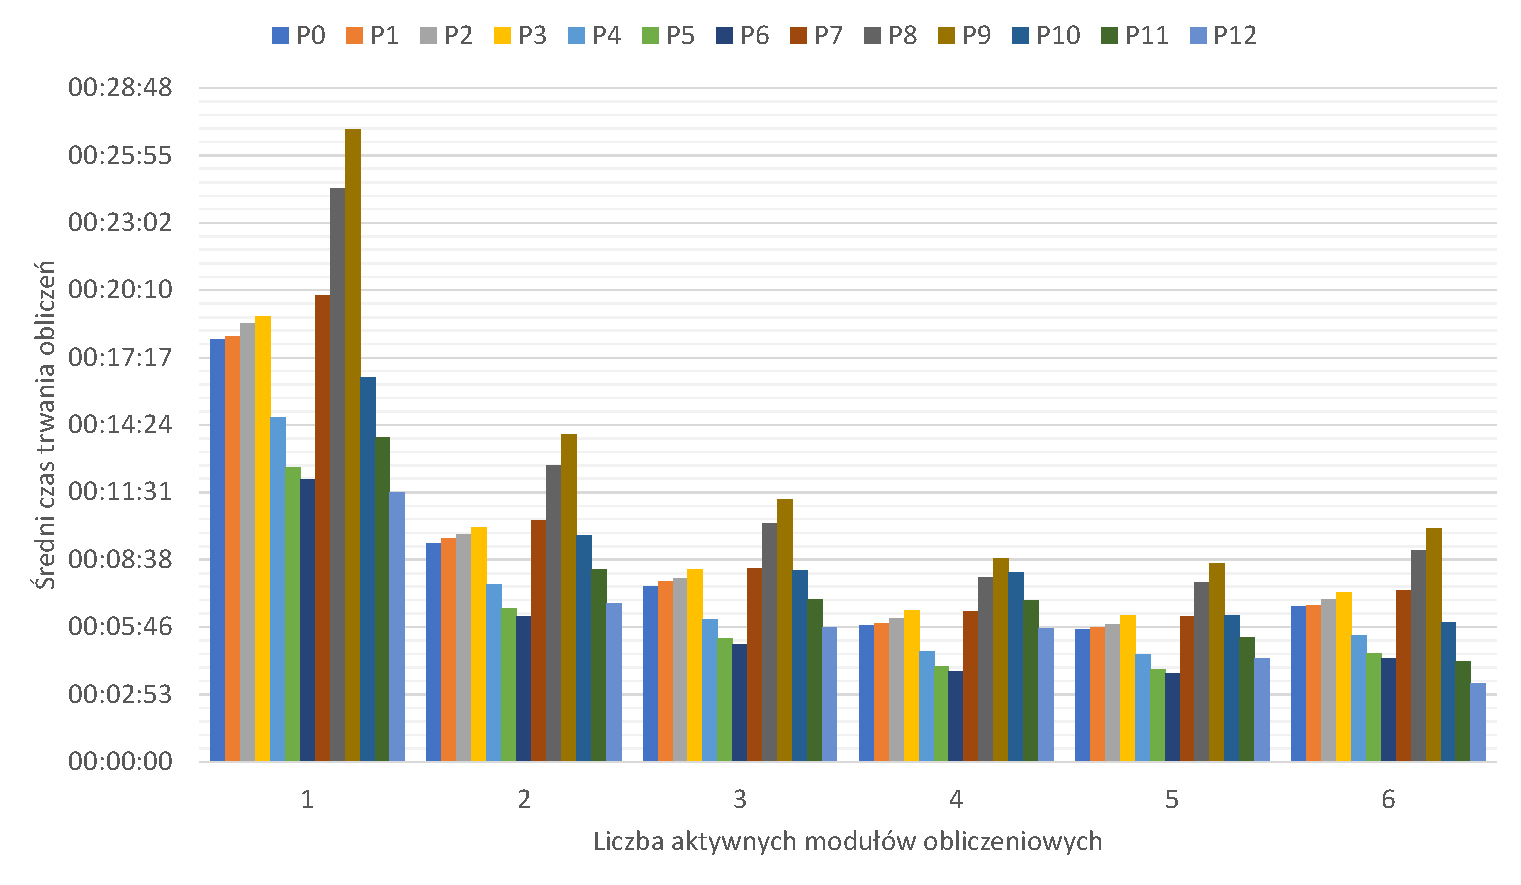
\includegraphics[width=.9\textwidth]{Chapters/Eksperymenty/scaling_results/p_proces.pdf}
\caption{Średni czas trwania obliczeń w zależności od liczby aktywnych modułów obliczeniowych dla wybranych scenariuszy testowych $P_0$ - $P_{12}$.}
\label{fig:chapter6:p_process}
\end{figure}


\bigbreak
Przeprowadzona analiza z wykorzystaniem dużej ilości danych w środowisku chmurowym (Rozdział \ref{sec:desc_skalowalnosc}) potwierdziła, że wytworzone oprogramowanie w ramach rozprawy doktorskiej z wykorzystaniem najnowszych technologii, takich jak Docker (Rozdział \ref{sec:docker}) oraz Kubernetes (\ref{sec:k8s}), przystosowane jest do przetwarzania przyrastającej ilości danych. Otrzymane czasy obliczeń dla wszystkich rozpatrywanych przypadków w porównaniu do czasu trwania skanowania oraz naprawy podatności są pomijalne, ponieważ, jak wykazano w rozdziale \ref{sec:desc_env_all}, czas skanowania oraz naprawy podatności liczony jest w godzinach. Na przykład najkrótszy czas skanowania otrzymany został dla środowiska teleinformatycznego A wynoszący 3 godziny. Natomiast czas naprawy podatności, jak przedstawiono w pracy \cite{farris2018vulcon}, mieści się w zakresie od 1 do 9 roboczogodzin. Ponadto opracowane oprogramowanie (Rozdział \ref{sec:scaling}) dla przypadku zwiększenia liczby aktywnych modułów obliczeniowych tylko o jeden, pozwala na zmniejszenie czasu przetwarzania danych aż o 45\%. W pełni zatem uzasadnione jest pominięcie w równaniach \ref{eq:cvss2e}, \ref{eq:cvss3e} czasu trwania wykonywania obliczeń ($T_{VMC}$). Dodatkowo w analizie wyłączono wszystkie możliwe optymalizacje dostarczane przez producentów wykorzystywanego oprogramowania Elasticsearch. W przypadku wykorzystania realnego środowiska z odpowiednio zaplanowaną architekturą możliwe jest otrzymanie jeszcze krótszych czasów obliczeń. Otrzymane wyniki pozwalają na stwierdzenie, że wykorzystując wytworzone oprogramowanie, możliwe jest rozwiązanie problemu przedstawionego w rozdziale \ref{sec:modele-zarzadzaia-podatnosciami}, dotyczącego skalowalności. Mianowicie wytworzone oprogramowanie dostosowane jest do rosnącej ilości napływających danych.

\bigbreak
Podsumowując, można stwierdzić, że dzięki wykorzystaniu zaimplementowanych rozwiązań przedstawionych w rozdziale drugim możliwa była istotna redukcja czasu obliczeń, ponieważ czas skanowania oraz naprawy podatności liczony jest w godzinach. Natomiast dla wszystkich analizowanych środowisk teleinformatycznych czas obliczeń z wykorzystaniem opracowanego oprogramowania wynosił poniżej minuty i nie miał większego wpływu na całościowy czas trwania procesu. Dlatego też w obliczeniach wykorzystujących równania \ref{eq:cvss2e} i \ref{eq:cvss3e}, dotyczących szacowanej liczby roboczogodzin wymaganych do usunięcia istotnych podatności bezpieczeństwa infrastruktury teleinformatycznych, można założyć, że $T_{VMC}$ = 0. W następnym podrozdziale przeprowadzono obliczenia szacowanej liczby roboczogodzin wymaganych do usunięcia istotnych podatności bezpieczeństwa dla trzech wybranych środowisk teleinformatycznych.

%%%%%%%%%%%%%%%%%%%%%%%%%%%%%%%%%%%%%%%%%%%%%%%%

%%%%%%%%%%%%%%%%%%%%%%%%%%%%%%%%%%%%%%%%%%%%%%%%
\section{Analiza zaproponowanych modeli zarządzania podatnościami}
Właściciele zasobów, od których pozyskano informacje na temat podatności znajdujących się w ich infrastrukturze (Rozdziały \ref{sec:desc_a}, \ref{sec:desc_b}, \ref{sec:desc_c}), nie wyrazili zgody na przetwarzanie danych w chmurze. Dlatego w celu przeprowadzenia analizy wykorzystano środowisko badawcze opisane w rozdziale \ref{sec:desc_pio}.

\bigbreak
Sposób przeprowadzenia analizy dla wszystkich środowisk teleinformatycznych wyglądał w następujący sposób:
\begin{enumerate}
    \item wczytanie raportu dotyczącego wykrytych podatności do narzędzia Nessus \cite{beale2004nessus},
    \item wczytanie danych dotyczących kategorii krytyczności dla analizowanego środowiska ICT do bazy inwentaryzacji zasobów Ralph \cite{ralph} (informacje otrzymane od administratorów),
    \item ręczne wymuszenie w panelu administratora wytworzonego na potrzeby pracy VMC, synchronizacji danych,
    \item analiza otrzymanych wyników.
\end{enumerate}

%%%%%%%%%%%%%%%%%%%%%%%%%%%%%%%%%%%%%%%%%%%%%%%%

%%%%%%%%%%%%%%%%%%%%%%%%%%%%%%%%%%%%%%%%%%%%%%%%
\subsection{Analiza dla środowiska teleinformatycznego A}

%%%%%%%%%%%%%%%%%%%%%%%%%%%%%%%%%%%%%%%%%%%%%%%%

%%%%%%%%%%%%%%%%%%%%%%%%%%%%%%%%%%%%%%%%%%%%%%%%
\subsubsection{Analiza wpływu parametrów środowiskowych na ocenę bazową CVSS 2.0}
\label{sec:analiza_cvss2_ev_a}
Rysunek \ref{fig:chapter6:env_a:cvss_2} przedstawia liczbę wykrytych podatności dla każdej kategorii krytyczności według oceny bazowej i środowiskowej CVSS 2.0. Na podstawie wyników pokazanych na rysunku \ref{fig:chapter6:env_a:cvss_2} można stwierdzić, że dla oceny środowiskowej CVSS 2.0 wszystkie podatności zostały przydzielone do kategorii niskiej. Wpływ na to ma parametr $TD$ (Rozdział \ref{sec:td}), który osiągnął maksymalną wartość 13\%, co zostało przedstawione na rysunku \ref{fig:chapter6:env_a:cvss_2_td}. Parametr $TD$ wskazuje procent zasobów wrażliwych na konkretną podatność. Rysunek \ref{fig:chapter6:env_a:cvss_2_td} przedstawia wartość parametru $TD$ dla wykrytych podatności w środowisku teleinformatycznym A. Wpływ pozostałych parametrów środowiskowych na kategorię krytyczności podatności, $CDP$ (Rozdział \ref{sec:cdp}) oraz $CIA$ (Rozdział \ref{sec:cia_desc}) jest niezauważalny, ponieważ parametr $TD$ osiąga maksymalną wartość 13\%. Wyniki przedstawione na rysunku \ref{fig:chapter6:env_a:cvss_2} potwierdzają, że model zarządzania podatnościami, który wykorzystuje ocenę środowiskową CVSS 2.0, ma istotną wadę. Wada ta polega na tym, że parametr $TD$, który służy do ustalania liczby systemów wrażliwych na daną podatność, znacząco zaniża oceny wszystkich podatności. Dlatego też model zarządzania podatnościami oparty o ocenę środowiskową CVSS 2.0 nie jest dokładną miarą bezpieczeństwa infrastruktury teleinformatycznej. Konieczne jest zatem rozważenie modelu zarządzania podatnościami, który opiera się na standardzie CVSS 3.x. Niemniej jednak należy zauważyć, że ocena środowiskowa CVSS 2.0 dostarcza bardzo ważnej informacji dla administratora. Mianowicie jeśli wartość parametru $TD$ jest niska, to w badanym środowisku teleinformatycznym wykryta podatność może zagrozić jedynie niewielkiej liczbie serwerów. Na przykład w środowisku A wykryto podatności, których wykorzystanie możne zagrozić co najwyżej 3 serwerom, tj. 13\% skanowanych zasobów.

\begin{figure}[!ht]
\centering
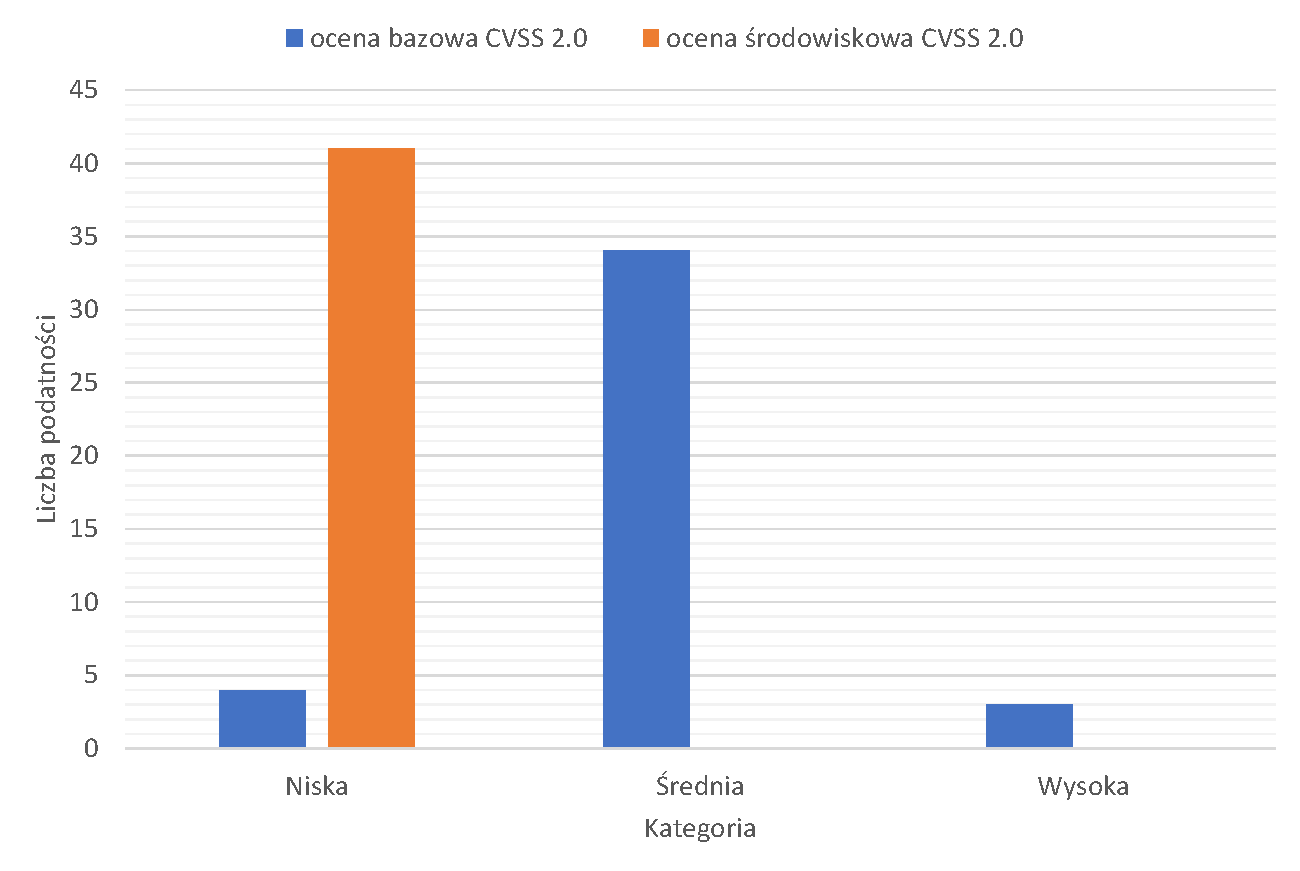
\includegraphics[width=.9\textwidth]{Chapters/Eksperymenty/env_A_results/cvss_2.pdf}
\caption{Liczba wykrytych podatności dla każdej kategorii krytyczności według oceny bazowej i środowiskowej CVSS 2.0 dla środowiska teleinformatycznego A.}
\label{fig:chapter6:env_a:cvss_2}
\end{figure}

\begin{figure}[!ht]
\centering
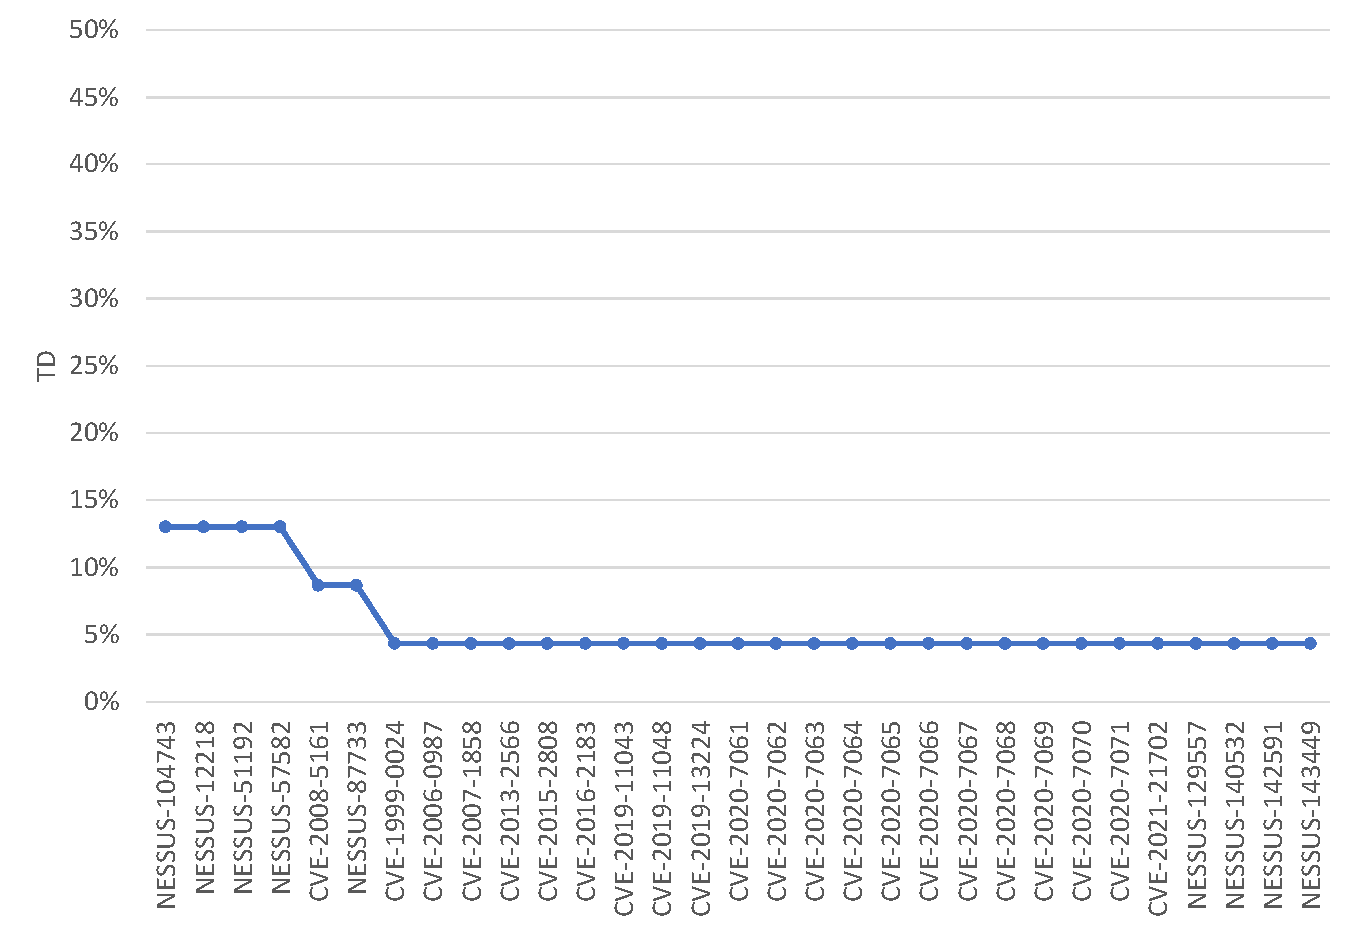
\includegraphics[width=.9\textwidth]{Chapters/Eksperymenty/env_A_results/cvss_2_td_env_a.pdf}
\caption{Wartość parametru $TD$ dla wykrytych podatności w środowisku teleinformatycznym A.}
\label{fig:chapter6:env_a:cvss_2_td}
\end{figure}

\bigbreak
Rysunek \ref{fig:chapter6:env_a:cvss_2_changes} przedstawia liczbę podatności zmodyfikowanych dla danej wartości różnicy pomiędzy oceną bazową a środowiskową CVSS 2.0 w przypadku środowiska teleinformatycznego A. Uwzględnienie parametrów środowiskowych $CIA$, $CDP$, $TD$ spowodowało zmianę wszystkich ocen bazowych CVSS 2.0 w przedziale od -8.9 do -2.4. Brak ocen bazowych niezmodyfikowanych spowodowany jest postacią równania \ref{eq:cvss2_es}, w którym to występuje mnożenie oceny końcowej przez wartość parametru środowiskowego $TD$, w celu otrzymania wartości oceny środowiskowej CVSS 2.0. Z liczby oraz zakresu zmian można wywnioskować, że w zbiorze wykrytych podatności znajdują się zagrożenia, które mogą mieć istotny wpływ na bezpieczeństwo monitorowanego środowiska. 

Zbiór wykrytych podatności w środowisku teleinformatycznym A składa się z dwóch podzbiorów: podatności posiadających obie oceny bazowe (CVSS 2.0 oraz CVSS 3.x) oraz podatności ze znaną jedynie oceną bazową w standardzie CVSS 2.0. W przypadku pierwszego podzbioru podatności posiadają ocenę bazową według standardu CVSS 3.x, w związku z czym priorytetyzacja naprawy zostanie ujęta w procesie zarządzania podatnościami za pomocą modelu \ref{fig:chapter1:vm-model-cvss3e} (Rozdział \ref{sec:proces-zarzadzania-podatnosciami}), ponieważ stosowanie oceny bazowej CVSS 3.x pozwala dokładniej ocenić krytyczność podatności, a zatem skuteczniej oszacować zagrożenia (Rozdział \ref{sec:modele-zarzadzaia-podatnosciami}). W przypadku drugiego podzbioru, który zawiera 14 (34\%) podatności, wykorzystano mechanizm konwersji oceny bazowej CVSS 2.0 do 3.x opisany w rozdziale \ref{sec:ml} w celu umożliwienia wykonania priorytetyzacji za pomocą modelu oceny środowiskowej CVSS 3.x (Rysunek \ref{fig:chapter1:vm-model-cvss3e}).

\begin{figure}[!ht]
\centering
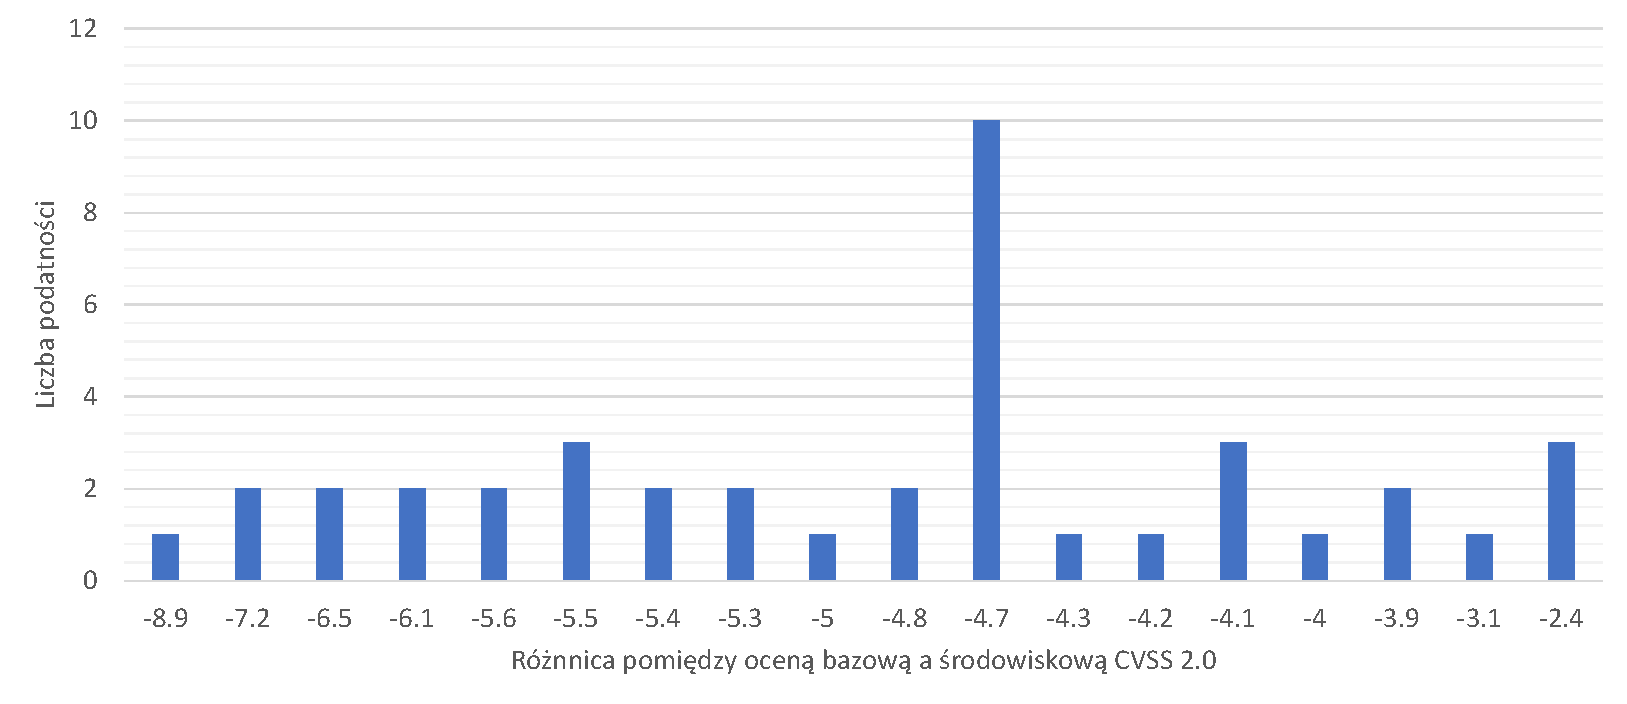
\includegraphics[width=.9\textwidth]{Chapters/Eksperymenty/env_A_results/changes_cvss_2.pdf}
\caption{Liczba podatności zmodyfikowanych dla danej wartości różnicy pomiędzy oceną bazową a środowiskową CVSS 2.0 w przypadku środowiska teleinformatycznego A.}
\label{fig:chapter6:env_a:cvss_2_changes}
\end{figure}

\bigbreak
Tabela \ref{tab:chapter6:env_a:time_results_cvss2} przedstawia liczbę roboczogodzin wymaganą do usunięcia istotnych podatności bezpieczeństwa dla środowiska teleinformatycznego A. W przypadku ocen bazowych CVSS 2.0 szacunkowa liczba roboczogodzin została obliczona za pomocą wzorów: $T_{Base2}$ - \ref{eq:cvss2}, $T_{Base2'}$ - \ref{eq:cvss2prim}. W przypadku oceny środowiskowej CVSS 2.0 szacunkowa liczba roboczogodzin została obliczona za pomocą wzoru \ref{eq:cvss2e}. Wartości dla czasów $T_{Base2}$ obliczone zostały przy założeniu, że administrator musi naprawić tylko podatności o krytyczności wysokiej i średniej, w związku z czym akceptuje ryzyko związane z istnieniem w systemie podatności o krytyczności niskiej. Ponadto należy zauważyć, ze w przypadku priortetyzacji opartej na ocenie bazowej CVSS 2.0, która nie uwzględnia danych środowiskowych wśród podatności sklasyfikowanych jako podatności o krytyczności niskiej mogą się znajdować podatności o wyższej krytyczności, na przykład wysokiej. Wartości czasów $T_{Base2'}$ obliczone zostały zatem przy założeniu, że w celu zapewnienia bezpieczeństwa systemu administrator musi naprawić wszystkie podatności, ponieważ (jak opisano szczegółowo w rozdziale \ref{sec:wplyw_cvss2}) nie ma pewności czy podatność z otrzymaną oceną bazową CVSS 2.0 zachowa tę ocenę po uwzględnieniu danych środowiskowych. Natomiast wartości dla czasów $T_{Env2}$ obliczone zostały przy założeniu, że wszystkie oceny podatności zostały sklasyfikowane dokładnie (Rozdział \ref{sec:modele-zarzadzaia-podatnosciami}). Gdy porówna się szacowane liczby roboczogodzin otrzymane dla $T_{Base2}$ z $T_{Base2'}$, można zauważyć wzrost szacowanej liczy roboczogodzin dla wszystkich rozpatrywanych przypadków ($T_{FIX_{MIN}}$, $T_{FIX_{AVERAGE}}$, $T_{FIX_{MAX}}$), który wynosi 10.4\%. Ponadto można zaobserwować, że naprawienie wszystkich podatności według otrzymanej priorytetyzacji za pomocą oceny bazowej CVSS 2.0 redukuje ryzyko nienaprawienia podatności niedoszacowanej z 10\% do 0\%. Gdy porównamy otrzymane wyniki dla $T_{Base2}$ i $T_{Env2}$, można zauważyć, że średni zysk w postaci obniżenia szacowanej liczby roboczogodzin dla wszystkich rozpatrywanych przypadków wynosi 95.8\%. Wykorzystanie priorytetyzacji za pomocą oceny środowiskowej CVSS 2.0 pozwala na obniżenie ryzyka związanego z nienaprawieniem podatności niedoszacowanej z 10\% do 0\%. Natomiast gdy porówna się wyniki otrzymane dla $T_{Base2'}$ i $T_{Env2}$, można zauważyć, że średni zysk w postaci obniżenia szacowanej liczby roboczogodzin dla wszystkich rozpatrywanych przypadków wynosi 96.9\% i tym samym utrzymuje ryzyko związane z nienaprawieniem podatności niedoszacowanych na poziomie 0\%.

\begin{table}[tbh]
\caption{Liczba roboczogodzin wymagana do usunięcia istotnych podatności bezpieczeństwa dla środowiska teleinformatycznego A. W przypadku ocen bazowych CVSS 2.0 szacunkowa liczba roboczogodzin została obliczona za pomocą wzorów: $T_{Base2}$ - \ref{eq:cvss2}, $T_{Base2'}$ - \ref{eq:cvss2prim}. W przypadku oceny środowiskowej CVSS 2.0 szacunkowa liczba roboczogodzin została obliczona za pomocą wzoru \ref{eq:cvss2e}.}
\begin{center}
\label{tab:chapter6:env_a:time_results_cvss2}
\begin{tabular}{c|ccc|c}
\hline
                & \textbf{$T_{FIX_{MIN}}$} & \textbf{$T_{FIX_{AVERAGE}}$} & \textbf{$T_{FIX_{MAX}}$ }  & Średnia \% zmiana \\
\hline
$T_{Base2}$      &                         40h &            169.5h &    336h         &        \\
$T_{Base2'}$     &                         44h &            187.5h &    372h         &         \\
Różnica          &               +4h (+10\%) &    +18h (+10.6\%) &  +36h (+10.7\%) & +10.4\%   \\  
\hline
$T_{Base2}$     &                          40h &            169.5h &    336h         &         \\
$T_{Env2}$        &                         3h &                3h &      3h         &         \\
Różnica          &              -37h (-92.5\%) & -166.5h (-98.5\%) & -333h (-99.1\%) & -95.8\% \\  
\hline
$T_{Base2'}$     &                         44h &            187.5h &    372h         &         \\
$T_{Env2}$        &                          3h &                3h &      3h        &         \\
Różnica          &              -41h (-93.2\%) & -184.5h (-98.4\%) & -368h (-99.2\%) & -96.9\% \\  
\hline
\end{tabular}
\end{center}
\end{table}

\bigbreak
Jak wykazano w przeprowadzonej analizie, model zarządzania podatnościami, który wykorzystuje ocenę środowiskową CVSS 2.0, ma istotną wadę. Wada ta polega na tym, że parametr $TD$, który służy do ustalania liczby systemów wrażliwych na daną podatność, znacząco zaniża oceny wszystkich wykrytych podatności. W analizowanym środowisku teleinformatycznym A spowodował sklasyfikowanie wszystkich podatności do kategorii niskiej. Dlatego też ocena środowiskowa CVSS 2.0 nie jest dokładną miarą bezpieczeństwa infrastruktury teleinformatycznej. Analiza wyników pozwala na wyciągnięcie kolejnego wniosku. Mianowicie model zarządzania podatnościami przy zastosowaniu oceny środowiskowej CVSS 2.0 (Rysunek \ref{fig:chapter1:vm-model-cvss2e}) może być wykorzystany do wykrywania podatności, które mogą zagrozić większej liczbie skanowanych zasobów. Taka informacja jest niezwykle cenna dla wszystkich osób zaangażowanych w proces zarządzania podatnościami (Rozdział \ref{sec:proces-zarzadzania-podatnosciami}), ponieważ pozwala na podjęcie szybkiej decyzji dotyczącej naprawy podatności oraz skrócenia czasu ich obecności w monitorowanej infrastrukturze teleinformatycznej.

%%%%%%%%%%%%%%%%%%%%%%%%%%%%%%%%%%%%%%%%%%%%%%%%

%%%%%%%%%%%%%%%%%%%%%%%%%%%%%%%%%%%%%%%%%%%%%%%%
\subsubsection{Analiza wpływu parametrów środowiskowych na ocenę bazową CVSS 3.x}

W celu wykonania analizy wpływu parametrów środowiskowych na ocenę bazową CVSS 3.x rozróżniono dwa przypadki. W pierwszym przypadku rozważane jest wykorzystanie metody konwersji ocen bazowych CVSS 2.0 do 3.x za pomocą uczenia maszynowego. W drugim przypadku rozważane jest brak metod konwersji i dopuszczany jest brak wiedzy na temat wszystkich ocen bazowych CVSS 3.x dla znacznej liczby wykrytych podatności.

\bigbreak
Dla pierwszego rozpatrywanego przypadku, w celu zapewnienia poprawnej priorytetyzacji wszystkich podatności za pomocą modeli zarządzania podatnościami wykorzystującymi CVSS 3.x (Rysunki \ref{fig:chapter1:vm-model-cvss3}, \ref{fig:chapter1:vm-model-cvss3e}), wykorzystano mechanizm konwersji CVSS 2.0 do CVSS 3.x za pomocą uczenia maszynowego (Rozdział \ref{sec:ml}), ponieważ 34\% podatności nie posiada oceny bazowej według CVSS 3.x dla środowiska teleinformatycznego A (Rozdział \ref{sec:desc_a}). W tabeli \ref{tab:chapter6:env_a:ml_classification} przedstawiono liczbę zmian dla każdej kategorii podatności według oceny bazowej CVSS 3.x w przypadku środowiska teleinformatycznego A po zastosowaniu mechanizmu konwersji oceny bazowej CVSS 2.0 do CVSS 3.x (ML) opartego na uczeniu maszynowym. Wykorzystany mechanizm uczenia maszynowego oblicza ocenę bazową CVSS 3.x obarczoną błędem klasyfikacji kategorii krytyczności wynoszącym 14\%, co oznacza, że można oczekiwać 2 podatności błędnie sklasyfikowanych w środowisku teleinformatycznym A.

\begin{table}[tbh]
\caption{Liczba zmian dla każdej kategorii podatności według oceny bazowej CVSS 3.x w przypadku środowiska teleinformatycznego A po zastosowaniu mechanizmu konwersji oceny bazowej CVSS 2.0 do CVSS 3.x (ML) opartego na uczeniu maszynowym.}
\begin{center}
\label{tab:chapter6:env_a:ml_classification}
\begin{tabular}{cccc}
\hline \noalign {\smallskip}
\textbf{Kategoria}  & \textbf{ocena bazowa} & \textbf{[ML] ocena bazowa} & \textbf{Różnica} \\
                      & \textbf{CVSS 3.x} & \textbf{CVSS 3.x} & \\
  \hline
  Niska         &      1 &      1  &  0          \\
                &        &         &  (0\%)     \\
  Średnia       &     14 &      23 &  +9           \\
                &        &         &  (+64.3\%)       \\
  Wysoka        &      6 &       8 &  +2           \\
                &        &         &  (+33.3\%)   \\
  Krytyczna     &      6 &      9  &  +3          \\
                &        &         &  (+50\%)   \\
\hline \noalign {\smallskip}
\textbf{Razem}  &     27 &       41& +14 \\
                &        &         & (+51.9\%) \\
\hline \noalign {\smallskip}
\end{tabular}
\end{center}
\end{table}

\bigbreak
Rysunek \ref{fig:chapter6:env_a:cvss_3} przedstawia liczbę wykrytych podatności dla każdej kategorii krytyczności według oceny bazowej i środowiskowej CVSS 3.x dla środowiska teleinformatycznego A dla obu rozpatrywanych przypadków. Na podstawie wyników pokazanych na rysunku \ref{fig:chapter6:env_a:cvss_3} można stwierdzić znaczącą zmianę w stosunku do oceny bazowej CVSS 3.x, która polega na zwiększeniu liczby podatności o kategorii krytycznej oraz zmniejszeniu liczby podatności o kategorii wysokiej. Wpływ na to mają ustawienia wartości parametrów środowiskowych $CIA$ dla 5 zasobów wskazanych przez administratora środowiska teleinformatycznego A o rozkładzie przedstawionym w tabeli \ref{tab:chapter5:env_a:cia}. Analiza wpływu parametrów środowiskowych $CIA$ na ocenę bazową CVSS 3.x przedstawiona została w rozdziale 4.

\begin{figure}[!ht]
\centering
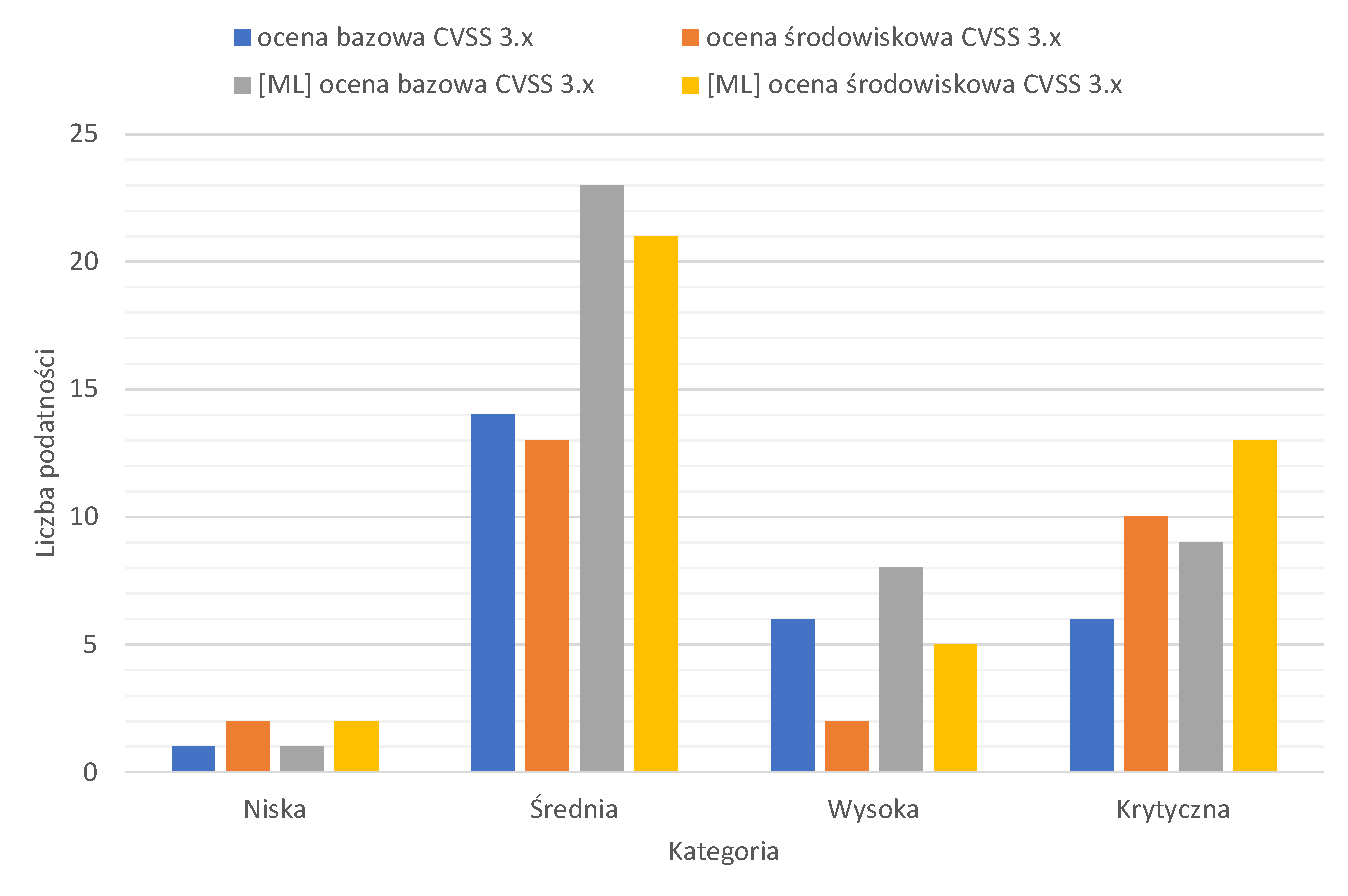
\includegraphics[width=.9\textwidth]{Chapters/Eksperymenty/env_A_results/cvss_3_ml.pdf}
\caption{Liczba wykrytych podatności dla każdej kategorii krytyczności według oceny bazowej i środowiskowej CVSS 3.x dla środowiska teleinformatycznego A.}
\label{fig:chapter6:env_a:cvss_3}
\end{figure}


\bigbreak
Rysunek \ref{fig:chapter6:env_a:cvss_3_changes_ml} przedstawia liczbę wszystkich podatności zmodyfikowanych dla danej wartości różnicy pomiędzy oceną bazową a środowiskową CVSS 3.x w przypadku środowiska teleinformatycznego A. Wyniki przedstawione na rysunku \ref{fig:chapter6:env_a:cvss_3_changes_ml} dotyczą rozpatrywanego przypadku pierwszego, w którym to uwzględnione są podatności z obliczoną oceną bazową CVSS 3.x za pomocą uczenia maszynowego. Parametry środowiskowe $CIA$ dla 5 wskazanych zasobów spowodowały modyfikację 19 ocen bazowych w zakresie od -2.1 do 1.9, co stanowi 46.3\% wszystkich wykrytych podatności. Pozostałe 22 podatności zostały wykryte na zasobach, dla których administrator środowiska A nie dostarczył żadnych informacji. 

\begin{figure}[!ht]
\centering
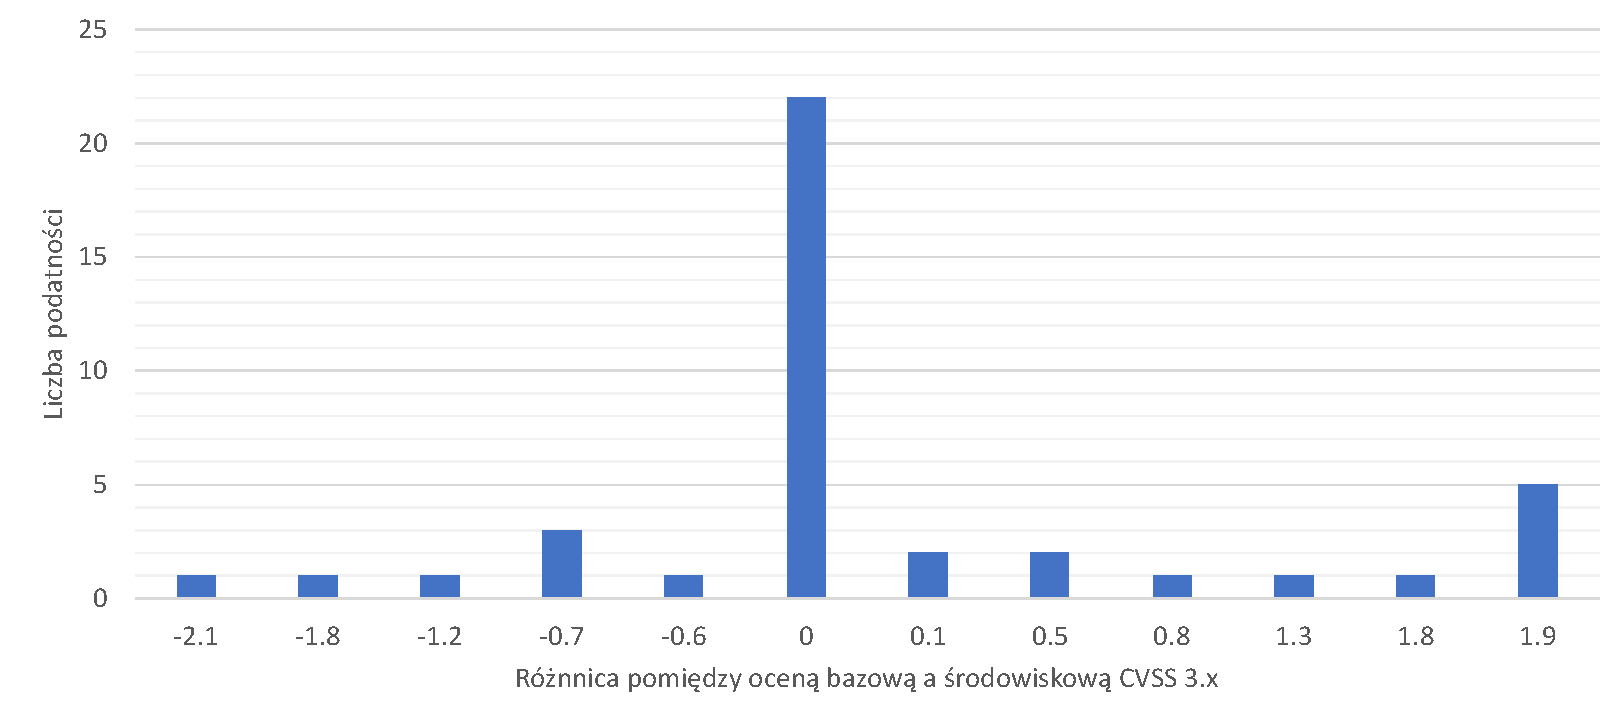
\includegraphics[width=.9\textwidth]{Chapters/Eksperymenty/env_A_results/changes_cvss_3_ml.pdf}
\caption{Liczba wszystkich podatności zmodyfikowanych dla danej wartości różnicy pomiędzy oceną bazową a środowiskową CVSS 3.x w przypadku środowiska teleinformatycznego A.}
\label{fig:chapter6:env_a:cvss_3_changes_ml}
\end{figure}

\bigbreak
Rysunek \ref{fig:chapter6:env_a:cvss_3_changes} przedstawia liczbę podatności zmodyfikowanych dla danej wartości różnicy pomiędzy oceną bazową a środowiskową CVSS 3.x w przypadku środowiska teleinformatycznego A. Wyniki przedstawione na rysunku \ref{fig:chapter6:env_a:cvss_3_changes} dotyczą rozpatrywanego przypadku drugiego, w którym to pomijane są podatności nie posiadające oceny bazowej CVSS 3.x. Parametry środowiskowe $CIA$ dla 5 wskazanych zasobów spowodowały modyfikacje 14 ocen bazowych w zakresie od -1.8 do 1.9, co stanowi 31.7\% wszystkich wykrytych podatności. Wyniki przedstawiające liczbę podatności zmodyfikowanych dla obu rozpatrywanych przypadków pozwalają na stwierdzenie, że każda informacja na temat środowiska może wpłynąć na zmianę w klasyfikacjach krytyczności podatności. Dodatkowo zmiana w klasyfikacjach krytyczności podatności wpływa na priorytetyzacje napraw podatności. Wykorzystanie mechanizmu konwersji oceny bazowej CVSS 2.0 do 3.x za pomocą uczenia maszynowego pozwala na uwzględnienie wszystkich wykrytych podatności w procesie zarządzania podatnościami dla analizowanego środowiska teleinformatycznego A.

\begin{figure}[!ht]
\centering
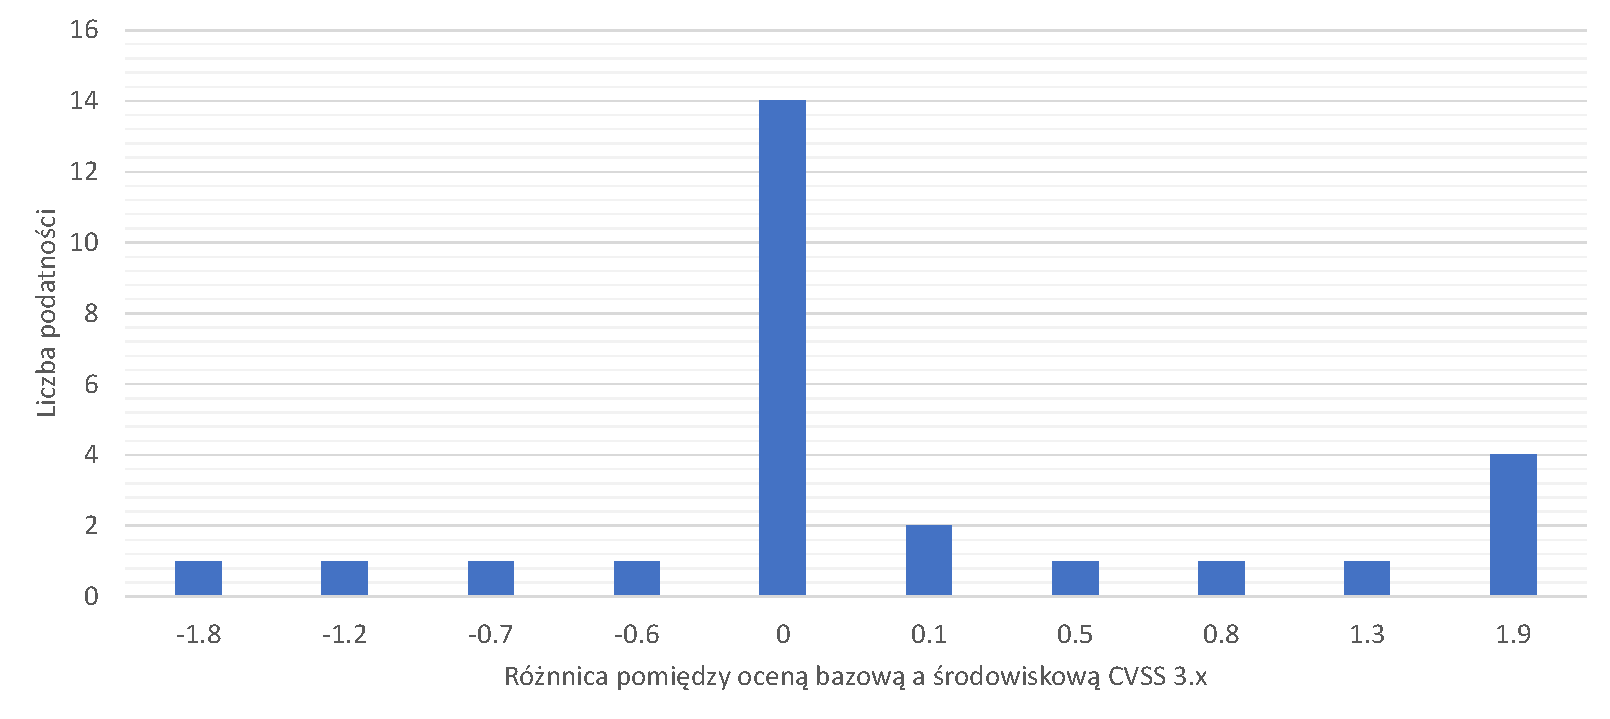
\includegraphics[width=.9\textwidth]{Chapters/Eksperymenty/env_A_results/changes_cvss_3.pdf}
\caption{Liczba podatności zmodyfikowanych dla danej wartości różnicy pomiędzy oceną bazową a środowiskową CVSS 3.x w przypadku środowiska teleinformatycznego A.}
\label{fig:chapter6:env_a:cvss_3_changes}
\end{figure}

\bigbreak
Tabela \ref{tab:chapter6:env_a:changes_ml} przedstawia liczbę zmian w kategoriach krytyczności podatności dla środowiska teleinformatycznego A po uwzględnieniu parametrów środowiskowych $CIA$ przy wykorzystaniu metod konwersji oceny bazowej CVSS 2.0 do 3.x za pomocą uczenia maszynowego. Największa zmiana w liczbie podatności została odnotowana dla kategorii krytycznej (+4) oraz wysokiej (-3). Dla zasobów posiadających wartości parametrów środowiskowych $CIA$ wykryto 29 podatności, co stanowi 70.71\% wszystkich podatności, 65.5\% z nich zmieniło swoją kategorię. W ogólnym ujęciu 24.39\% podatności zmieniło swoją kategorię z powodu wpływu wartości parametrów środowiskowych $CIA$ dla 5 zasobów. Uzyskane wyniki pozwalają na wyciągnięcie dwóch wniosków. Pierwszy mówi o tym, że możliwe jest wykorzystanie mechanizmu konwersji oceny bazowej CVSS 2.0 do 3.x do pełnej implementacji modelu zarządzania podatnościami opartego na ocenie środowiskowej CVSS 3.x dla wszystkich podatności. Natomiast drugi wniosek pozwala na stwierdzenie, że każda dodatkowa informacja na temat monitorowanego środowiska wpływa na priorytetyzacje napraw podatności poprzez możliwość zmiany kategorii krytyczności podatności.


\begin{table}[tbh]
\caption{Liczba zmian w kategoriach podatności dla środowiska teleinformatycznego A z wykorzystaniem metod konwersji oceny bazowej CVSS 2.0 do CVSS 3.x za pomocą uczenia maszynowego.}
\begin{center}
\label{tab:chapter6:env_a:changes_ml}
\begin{tabular}{cccc}
\hline \noalign {\smallskip}
\textbf{Kategoria}  & \textbf{[ML] ocena bazowa} & \textbf{[ML] ocena środowiskowa} & \textbf{Różnica} \\
                      & \textbf{CVSS 3.x} & \textbf{CVSS 3.x} & \\
  \hline
  Niska         &      1 &      2  &  +1          \\
                &        &         &  (+100\%)     \\
  Średnia       &     23 &      21 &  -2           \\
                &        &         &  (-8.69\%)       \\
  Wysoka        &      8 &       5 &  -3           \\
                &        &         &  (-37.5\%)   \\
  Krytyczna     &      9 &      13 &  +4          \\
                &        &         &  (+44.44\%)   \\
\hline \noalign {\smallskip}
\textbf{Razem}  &     41 &       41& 10 \\
                &        &         & (24.39\%) \\
\hline \noalign {\smallskip}
\end{tabular}
\end{center}
\end{table}

\bigbreak
Tabela \ref{tab:chapter6:env_a:changes} przedstawia liczbę zmian w kategoriach krytyczności podatności po uwzględnieniu parametrów środowiskowych $CIA$ dla środowiska teleinformatycznego A. Wyniki przedstawione w tabeli \ref{tab:chapter6:env_a:changes} nie uwzględniają mechanizmu konwersji oceny bazowej CVSS 2.0 do 3.x za pomocą uczenia maszynowego, to znaczy, że nie obejmują podatności, które nie posiadają oceny bazowej CVSS 3.x. Największa zmiana w liczbie podatności została odnotowana dla kategorii krytycznej (+4) oraz wysokiej (-4). Dla zasobów posiadających wartości parametrów środowiskowych $CIA$ wykryto 22 podatności, co stanowi 53.7\% wszystkich podatności, 59.1\% z nich zmieniło swoją kategorię. W ogólnym ujęciu 37\% podatności zmieniło swoją kategorię z powodu wpływu wartości parametrów środowiskowych $CIA$ dla 5 zasobów. Pomimo nieuwzględnienia wszystkich wykrytych podatności, parametry środowiskowe $CIA$ spowodowały znaczą zmianę w kategoriach krytyczności. Uzyskane wyniki pozwalają na wyciągnięcie wniosku mówiącego o tym, że znajomość parametrów środowiskowych $CIA$ tylko dla części monitorowanych zasobów pozwala na lepsze dopasowanie podatności, nawet w przypadku, gdy administrator akceptuje ryzyko, w którym pomija naprawę podatności nie posiadające ocenę bazową CVSS 3.x.

\begin{table}[tbh]
\caption{Liczba zmian w kategoriach podatności po uwzględnieniu parametrów środowiskowych $CIA$ dla środowiska teleinformatycznego A.}
\begin{center}
\label{tab:chapter6:env_a:changes}
\begin{tabular}{cccc}
\hline \noalign {\smallskip}
\textbf{Kategoria} & \textbf{ocena bazowa} & \textbf{ocena środowiskowa} & \textbf{Różnica} \\
                      & \textbf{CVSS 3.x} & \textbf{CVSS 3.x} & \\
  \hline
  Niska         &      1 &      2  &  +1          \\
                &        &         &  (+100\%)     \\
  Średnia       &     14 &      13 &  -1           \\
                &        &         &  (-7.1\%)       \\
  Wysoka        &      6 &       2 &  -4           \\
                &        &         &  (-66.7\%)   \\
  Krytyczna     &      6 &      10 &  +4          \\
                &        &         &  (+66.7\%)   \\
\hline \noalign {\smallskip}
\textbf{Razem}  &     27 &      27 & 10 \\
                &        &         & (37\%) \\
\hline \noalign {\smallskip}
\end{tabular}
\end{center}
\end{table}

\bigbreak
Tabela \ref{tab:chapter6:env_a:time_results_cvss_3} przedstawia liczbę roboczogodzin wymaganą do usunięcia istotnych podatności bezpieczeństwa dla środowiska teleinformatycznego A. W przypadku ocen bazowych CVSS 3.x szacunkowa liczba roboczogodzin została obliczona za pomocą wzorów: $T_{Base3}$ - \ref{eq:cvss3}, $T_{Base3'}$ - \ref{eq:cvss2prim}. W przypadku oceny środowiskowej CVSS 3.x szacunkowa liczba roboczogodzin została obliczona za pomocą wzoru \ref{eq:cvss3e}. Wartości dla czasów $T_{Base3}$ obliczone zostały przy założeniu, że administrator musi naprawić tylko podatności o kategorii krytycznej, wysokiej i średniej, w związku z czym akceptuje ryzyko związane z istnieniem w systemie podatności o krytyczności niskiej. Ponadto należy zauważyć, że w przypadku priortetyzacji opartej na ocenie bazowej CVSS 3.x, która nie uwzględnia danych środowiskowych wśród podatności sklasyfikowanych jako podatności o krytyczności niskiej, mogą się znajdować podatności o wyższej krytyczności, na przykład wysokiej. Wartości czasów $T_{Base3'}$ obliczone zostały zatem przy założeniu, że w celu zapewnienia bezpieczeństwa systemu administrator musi naprawić wszystkie podatności, ponieważ (jak opisano szczegółowo w rozdziale \ref{sec:wplyw_cvss3}) nie ma pewności, czy podatność z otrzymaną oceną bazową CVSS 3.x zachowa tę ocenę po uwzględnieniu danych środowiskowych. Natomiast wartości dla czasów $T_{Env3}$ obliczone zostały przy założeniu, że wszystkie oceny podatności zostały sklasyfikowane dokładnie (Rozdział \ref{sec:modele-zarzadzaia-podatnosciami}). Gdy porówna się szacowane liczby roboczogodzin otrzymane dla $T_{Base3}$ z $T_{Base3'}$, można zauważyć wzrost szacowanej liczy roboczogodzin dla wszystkich rozpatrywanych przypadków ($T_{FIX_{MIN}}$, $T_{FIX_{AVERAGE}}$, $T_{FIX_{MAX}}$), który wynosi 3.7\%. Ponadto można zaobserwować, że naprawienie wszystkich podatności według otrzymanej priorytetyzacji za pomocą oceny bazowej CVSS 3.x redukuje ryzyko nienaprawienia podatności niedoszacowanej z 34.1\% do 31.7\%. Gdy porówna się otrzymane wyniki dla $T_{Base3}$ i $T_{Env3}$, można zauważyć, że średni zysk w postaci obniżenia szacowanej liczby roboczogodzin dla wszystkich rozpatrywanych przypadków wynosi 3.8\%. Wykorzystanie priorytetyzacji za pomocą oceny środowiskowej CVSS 3.x obniża ryzyko z związane z nienaprawieniem podatności niedoszacowanej z 34.1\% do 29.1\%. Natomiast gdy porówna się wyniki otrzymane dla $T_{Base3'}$ i $T_{Env3}$, można zauważyć średni zysk w postaci obniżenia szacowanej liczby roboczogodzin dla wszystkich rozpatrywanych przypadków wynoszący 7\%. Ponadto wykonanie napraw podatności za pomocą prioretetyzacji podatności według oceny środowiskowej CVSS 3.x powoduje utrzymanie ryzyka dotyczącego wykorzystania nienaprawionej podatności przez atakującego na poziomie 29.1\%. W przypadku wykorzystania metod konwersji CVSS 2.0 do CVSS 3.x za pomocą uczenia maszynowego otrzymane wyniki dla $T_{Base3}$ i $T_{Base3ML}$ przedstawiają wzrost szacowanej liczby roboczogodzin o 51\%. Dodatkowo wykorzystanie metod konwersji oceny bazowej CVSS 2.0 do 3.x powoduje redukcję ryzyka dotyczącego możliwości wykorzystania podatności nienaprawionej przez atakującego z 34.1\% do 2.4\%. Natomiast gdy porówna się otrzymane wyniki dla $T_{Base3}$ i $T_{Env3ML}$, możemy zauważyć wzrost szacowanej liczby roboczogodzin o 47.6\%. Dodatkowo wykonanie pioretetyzacji napraw podatności za pomocą oceny środowiskowej CVSS 3.x z wykorzystaniem metod konwersji oceny bazowej CVSS 3.x redukuje ryzyko dotyczące nienaprawienia podatności, która może zostać wykorzystana przez atakującego, z 34.1\% do 2.4\%.

\begin{table}[tbh]
\caption{Liczba roboczogodzin wymagana do usunięcia istotnych podatności bezpieczeństwa dla środowiska teleinformatycznego A. W przypadku ocen bazowych CVSS 3.x szacunkowa liczba roboczogodzin została obliczona za pomocą wzorów: $T_{Base3}$ - \ref{eq:cvss3}, $T_{Base3'}$ - \ref{eq:cvss2prim}. W przypadku oceny środowiskowej CVSS 3.x szacunkowa liczba roboczogodzin została obliczona za pomocą wzoru \ref{eq:cvss3e}.}
\begin{center}
\label{tab:chapter6:env_a:time_results_cvss_3}
\begin{tabular}{c|ccc|c}
\hline
                 & \textbf{$T_{FIX_{MIN}}$} & \textbf{$T_{FIX_{AVERAGE}}$} & \textbf{$T_{FIX_{MAX}}$ }  & Średnia \% zmiana \\
\hline
$T_{Base3}$      &                         29h &              120h &    237h         &        \\
$T_{Base3'}$     &                         30h &            124.5h &    246h         &         \\
Różnica          &                +1h (+3.4\%) &    +4.5h (+3.7\%) &  +9h (+3.8\%) & +3.7\%   \\  
\hline
$T_{Base3}$      &                         29h &            120h &      237h         &        \\
$T_{Env3}$       &                         28h &            115.5h &    228h         &         \\
Różnica          &                -1h (-3.4\%) &    -4.5h (-3.8\%) &  -9h (-3.8\%) & -3.8\%   \\  
\hline
$T_{Base3'}$     &                         30h &            124.5h &    246h         &        \\
$T_{Env3}$       &                         28h &            115.5h &    228h         &         \\
Różnica          &                -2h (-6.6\%) &    -9h (-7.2\%) &  -18h (-7.3\%) & -7\%   \\  
\hline
$T_{Base3}$    &                      29h &            120h &    237h         &         \\
$T_{Base3ML}$&                        43h &          183h &      363h         &         \\
Różnica          &              +14h (+48\%) & +63h (+52\%) & +126h (+53\%) & +51\% \\  
\hline
$T_{Base3}$  &                             29h &            120h &    237h        &         \\
$T_{Env3ML}$     &                         42h &          178.5h &    354h        &         \\
Różnica          &               +13h (+44.8\%)  &  +58.5h (+48.5\%) & +117h (+49.3\%) & +47.6\% \\  
\hline
$T_{Base3ML}$    &                         43h &            183h &    363h         &         \\
$T_{Env3ML}$     &                         42h &          178.5h &    354h        &         \\
Różnica          &               -1h (-2.3\%)  &  -4.5h (-2.6\%) & -9h (-2.5\%) & -2.4\% \\  
\hline
\end{tabular}
\end{center}
\end{table}

\bigbreak
Jak wykazano w przeprowadzonej analizie, parametry środowiskowe $CIA$ mają znaczący wpływ na priorytetyzacje podatności bezpieczeństwa infrastruktury informatycznej, pomimo posiadania parametrów środowiskowych $CIA$ tylko dla 5 skanowanych zasobów. Parametry środowiskowe $CIA$ mają wpływ na szacowaną liczbę roboczogodzin wymaganą do usunięcia istotnych podatności bezpieczeństwa środowiska teleinformatycznego A w procesie zarządzania podatnościami (Rozdział \ref{sec:proces-zarzadzania-podatnosciami}). Wykorzystanie modelu zarządzania podatnościami opartego na ocenie środowiskowej CVSS 3.x (Rysunek \ref{fig:chapter1:vm-model-cvss3e}) z metodami konwersji oceny bazowej CVSS 2.0 do 3.x pozwala na lepsze dopasowanie kategorii podatności, a tym samym wpływa na priorytetyzacje napraw podatności dla otrzymanych danych, opisanych w rozdziale \ref{sec:desc_a}. Jak wynika z przeprowadzonej analizy, możliwe jest otrzymanie wyników oceny środowiskowej niezwłocznie po zakończonym procesie skanowania, co w rezultacie daje zysk w postaci obniżenia szacowanej liczby roboczogodzin o 7\%, oraz redukcje ryzyka nienaprawionych podatności niedoszacowanych z 34.1\% do 29.1\%. W przypadku wykorzystania metod konwersji CVSS 2.0 do CVSS 3.x możliwa jest redukcja ryzyka nienaprawienia podatności niedoszacowanych z 34.1\% do 2.4\%, jednocześnie obniżając szacowaną liczbę roboczogodzin potrzebnych do naprawienia wszystkich podatności o 2.4\%.

%%%%%%%%%%%%%%%%%%%%%%%%%%%%%%%%%%%%%%%%%%%%%%%%

%%%%%%%%%%%%%%%%%%%%%%%%%%%%%%%%%%%%%%%%%%%%%%%%

\subsubsection{Podsumowanie wyników analizy dla środowiska A}
Na podstawie wyników przedstawionych w podrozdziale ''Analiza wpływu parametrów środowiskowych na ocenę bazową CVSS 2.0'' można stwierdzić, że dla oceny środowiskowej wszystkie podatności zostały przydzielone do kategorii niskiej. Wpływ na to ma parametr $TD$, który osiągnął maksymalną wartość 13\%. Dodatkowo z analizy otrzymanych wyników można stwierdzić, że dodanie do oceny bazowej CVSS 2.0 danych środowiskowych powoduje znaczącą redukcję szacowanej liczby roboczogodzin wymaganą do usunięcia istotnych podatności wykrytych w środowisku teleinformatycznym A. Gdy porównamy wyniki otrzymane dla oceny bazowej CVSS 2.0 ($T_{Base2}$) z oceną środowiskową CVSS 2.0 ($T_{Env2}$), można zauważyć, że średni zysk w postaci obniżenia szacowanej liczby roboczogodzin wynosi 95.8\%. Wykorzystanie priorytetyzacji za pomocą oceny środowiskowej CVSS 2.0 pozwala na obniżenie ryzyka związanego z nienaprawieniem podatności niedoszacowanej z 10\% do 0\%. Wyniki przedstawione w podrozdziale ''Analiza wpływu parametrów środowiskowych na ocenę bazową CVSS 2.0'' potwierdzają wadę oceny środowiskowej CVSS 2.0 polegającą na tym, że parametr $TD$, który służy do ustalania liczby systemów wrażliwych na daną podatność, znacząco zaniża oceny wszystkich podatności. Dlatego konieczne było rozważenie modelu zarządzania podatnościami, który opiera się na standardzie CVSS 3.x.

\bigbreak
Na podstawie wyników przedstawionych w podrozdziale ''Analiza wpływu parametrów środowiskowych na ocenę bazową CVSS 3.x'' można stwierdzić, że wykorzystany mechanizm uczenia maszynowego wykonał obliczenia dla 34\% podatności wykrytych w środowisku teleinformatycznym A, które nie posiadają oceny bazowej CVSS 3.x z błędem klasyfikacji kategorii krytyczności wynoszącym 14\%, co oznacza, że można oczekiwać 2 podatności błędnie sklasyfikowanych, pozwalając tym samym na pełną implementację modelu zarządzania podatnościami opartego na standardzie CVSS 3.x (Rysunek \ref{fig:chapter1:vm-model-cvss3}, \ref{fig:chapter1:vm-model-cvss3e}). Z analizy otrzymanych wyników można także stwierdzić, że wpływ parametrów środowiskowych $CIA$ spowodował zmianę kategorii krytyczności dla 24.39\% podatności, co ma bezpośredni przekład na szacowaną liczbę roboczogodzin potrzebną do usunięcia istotnych podatności wykrytych w środowisku teleinformatycznym A. Gdy porównamy wyniki otrzymane dla oceny bazowej CVSS 3.x bez zastosowania metod konwersji oceny bazowej CVSS 2.0 do 3.x ($T_{Base3}$) z oceną środowiskową CVSS 3.x z zastosowaniem metod konwersji oceny bazowej CVSS 2.0 do 3.x. ($T_{Env3ML}$), można zauważyć wzrost szacowanej liczby roboczogodzin o 47.6\%. Wzrost szacowanej liczby roboczogodzin wynika z uwzględnienia wszystkich podatności po zastosowaniu metod konwersji oceny bazowej CVSS 2.0 do 3.x za pomocą uczenia maszynowego. Natomiast wykonanie priorytetyzacji napraw podatności za pomocą oceny środowiskowej CVSS 3.x z wykorzystaniem metod konwersji oceny bazowej CVSS 2.0 do 3.x redukuje ryzyko dotyczące nienaprawienia podatności, która może zostać wykorzystana przez atakującego, z 34.1\% do 2.4\%.

%%%%%%%%%%%%%%%%%%%%%%%%%%%%%%%%%%%%%%%%%%%%%%%%

%%%%%%%%%%%%%%%%%%%%%%%%%%%%%%%%%%%%%%%%%%%%%%%%
\subsection{Analiza dla środowiska teleinformatycznego B}


%%%%%%%%%%%%%%%%%%%%%%%%%%%%%%%%%%%%%%%%%%%%%%%%

%%%%%%%%%%%%%%%%%%%%%%%%%%%%%%%%%%%%%%%%%%%%%%%%
\subsubsection{Analiza wpływu parametrów środowiskowych na ocenę bazową CVSS 2.0}

Rysunek \ref{fig:chapter6:env_b:cvss_2} przedstawia liczbę wykrytych podatności dla każdej kategorii krytyczności według oceny bazowej i środowiskowej CVSS 2.0. Na podstawie wyników pokazanych na rysunku \ref{fig:chapter6:env_b:cvss_2} można stwierdzić, że dla oceny środowiskowej CVSS 2.0 znaczna większość podatności została przydzielona do kategorii niskiej. Wpływ na to ma parametr $TD$ (Rozdział \ref{sec:td}), który osiągnął maksymalną wartość 25\%, co zostało przedstawione na rysunku \ref{fig:chapter6:env_b:cvss_2_td}. Parametr $TD$ wskazuje procent zasobów wrażliwych na konkretną podatność. Rysunek \ref{fig:chapter6:env_b:cvss_2_td} przedstawia wartość parametru $TD$ dla wykrytych podatności w środowisku teleinformatycznym A. Wpływ pozostałych parametrów środowiskowych na kategorię krytyczności podatności, $CDP$ (Rozdział \ref{sec:cdp}) oraz $CIA$ (Rozdział \ref{sec:cia_desc}) jest niezauważalny, ponieważ parametr $TD$ osiąga maksymalną wartość 25\%. Wyniki przedstawione na rysunku \ref{fig:chapter6:env_b:cvss_2} potwierdzają, że model zarządzania podatnościami, który wykorzystuje ocenę środowiskową CVSS 2.0, ma istotną wadę. Wada ta polega na tym, że parametr $TD$, który służy do ustalania liczby systemów wrażliwych na daną podatność, znacząco zaniża oceny wszystkich podatności. Dlatego też model zarządzania podatnościami oparty o ocenę środowiskową CVSS 2.0, nie jest dokładną miarą bezpieczeństwa infrastruktury teleinformatycznej. Konieczne jest zatem rozważenie modelu zarządzania podatnościami, który opiera się na standardzie CVSS 3.x. Niemniej jednak należy zauważyć, że ocena środowiskowa CVSS 2.0 dostarcza bardzo ważnej informacji dla administratora. Mianowicie jeśli wartość parametru $TD$ jest niska, to w badanym środowisku teleinformatycznym wykryta podatność może zagrozić jedynie niewielkiej liczbie serwerów. Na przykład w środowisku C wykryto podatności, których wykorzystanie możne zagrozić co najwyżej 9 serwerom, tj. 25\% skanowanych zasobów.

\begin{figure}[!ht]
\centering
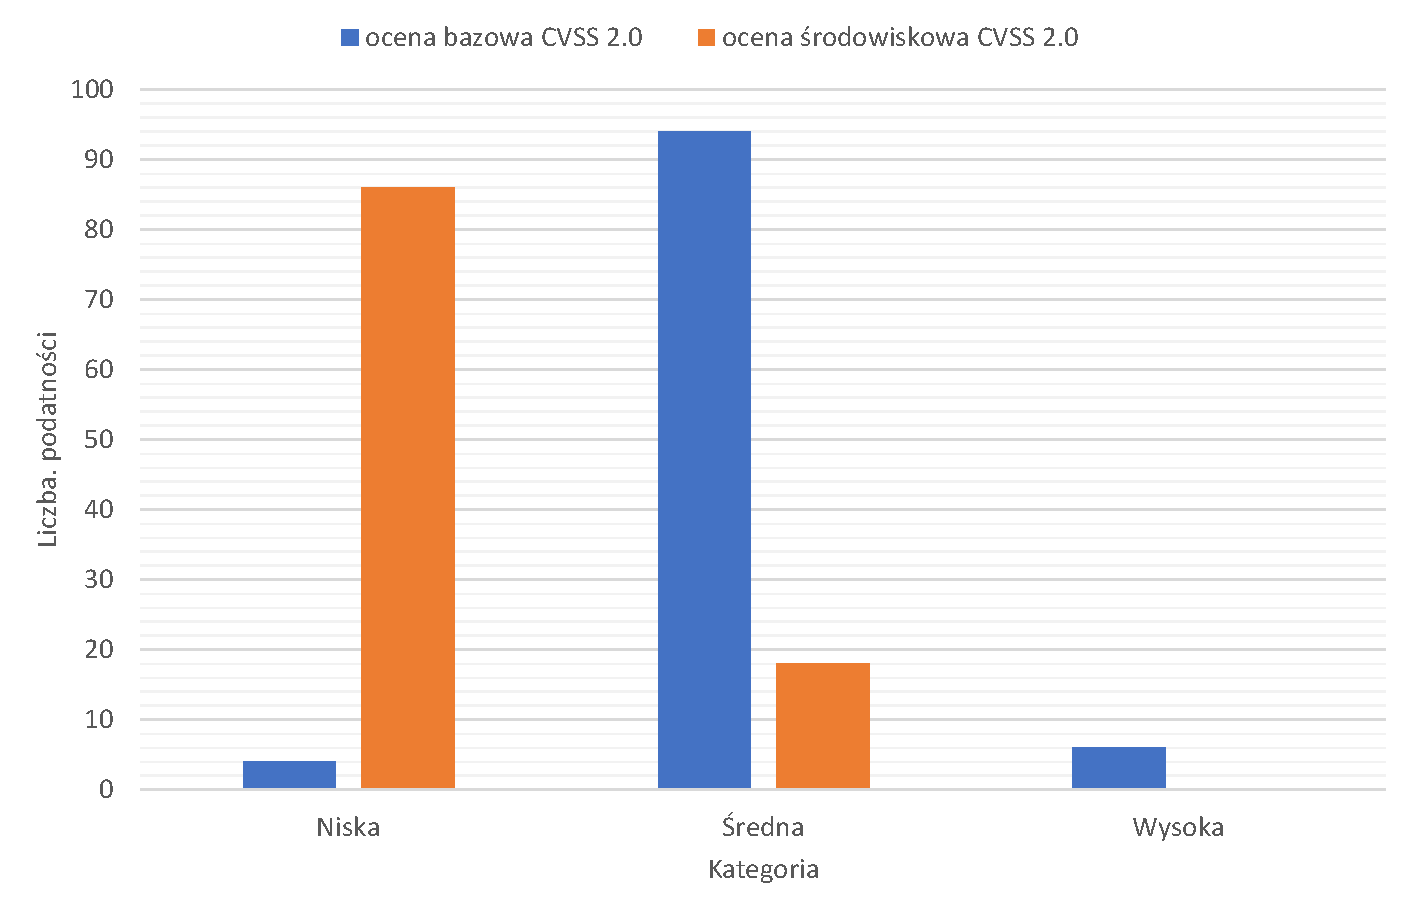
\includegraphics[width=.9\textwidth]{Chapters/Eksperymenty/env_B_results/cvss_2.pdf}
\caption{Liczba wykrytych podatności dla każdej kategorii krytyczności według oceny bazowej i środowiskowej CVSS 2.0 dla środowiska teleinformatycznego B.}
\label{fig:chapter6:env_b:cvss_2}
\end{figure}

\begin{figure}[!ht]
\centering
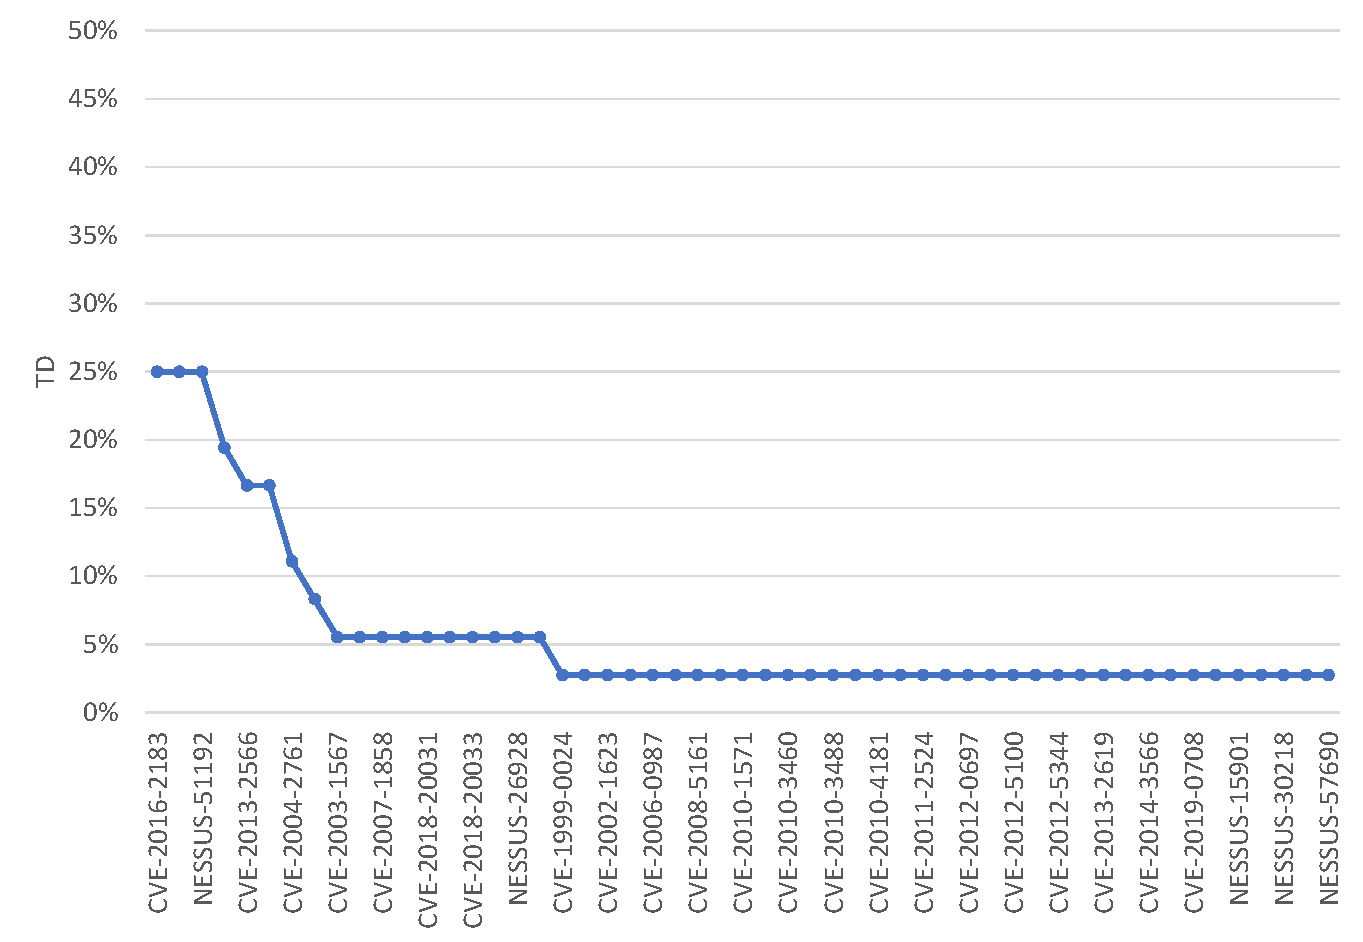
\includegraphics[width=.9\textwidth]{Chapters/Eksperymenty/env_B_results/cvss_2_td_env_b.pdf}
\caption{Wartość parametru $TD$ dla wykrytych podatności w środowisku teleinformatycznym B.}
\label{fig:chapter6:env_b:cvss_2_td}
\end{figure}

\bigbreak
Rysunek \ref{fig:chapter6:env_b:cvss_2_changes} przedstawia liczbę podatności zmodyfikowanych dla danej wartości różnicy pomiędzy oceną bazową a środowiskową CVSS 2.0 w przypadku środowiska teleinformatycznego B. Uwzględnienie parametrów środowiskowych $CIA$, $CDP$, $TD$ spowodowało zmianę wszystkich ocen bazowych CVSS 2.0 w przedziale od -7.5 do -1.2. Brak ocen bazowych niezmodyfikowanych spowodowany jest postacią równania \ref{eq:cvss2_es}, w którym to występuje mnożenie oceny końcowej przez wartość parametru środowiskowego $TD$ w celu otrzymania wartości oceny środowiskowej CVSS 2.0. Z liczby oraz zakresu zmian można wywnioskować, że w zbiorze wykrytych podatności znajdują się zagrożenia, które mogą mieć istotny wpływ na bezpieczeństwo monitorowanego środowiska. 

Zbiór wykrytych podatności w środowisku teleinformatycznym B składa się z dwóch podzbiorów: podatności posiadających obie oceny bazowe (CVSS 2.0 oraz CVSS 3.x) oraz podatności ze znaną jedynie oceną bazową w standardzie CVSS 2.0. W przypadku pierwszego podzbioru podatności posiadają ocenę bazową według standardu CVSS 3.x, w związku z czym priorytetyzacja naprawy zostanie ujęta w procesie zarządzania podatnościami za pomocą modelu \ref{fig:chapter1:vm-model-cvss3e} (Rozdział \ref{sec:proces-zarzadzania-podatnosciami}), ponieważ stosowanie oceny bazowej CVSS 3.x pozwala dokładniej ocenić krytyczność podatności, a zatem skuteczniej oszacować zagrożenia (Rozdział \ref{sec:modele-zarzadzaia-podatnosciami}). W przypadku drugiego podzbioru, który zawiera 50 (48\%) podatności, wykorzystano mechanizm konwersji oceny bazowej CVSS 2.0 do 3.x opisany w rozdziale \ref{sec:ml} w celu umożliwienia wykonania priorytetyzacji za pomocą modelu oceny środowiskowej CVSS 3.x (Rysunek \ref{fig:chapter1:vm-model-cvss3e}).

\begin{figure}[!ht]
\centering
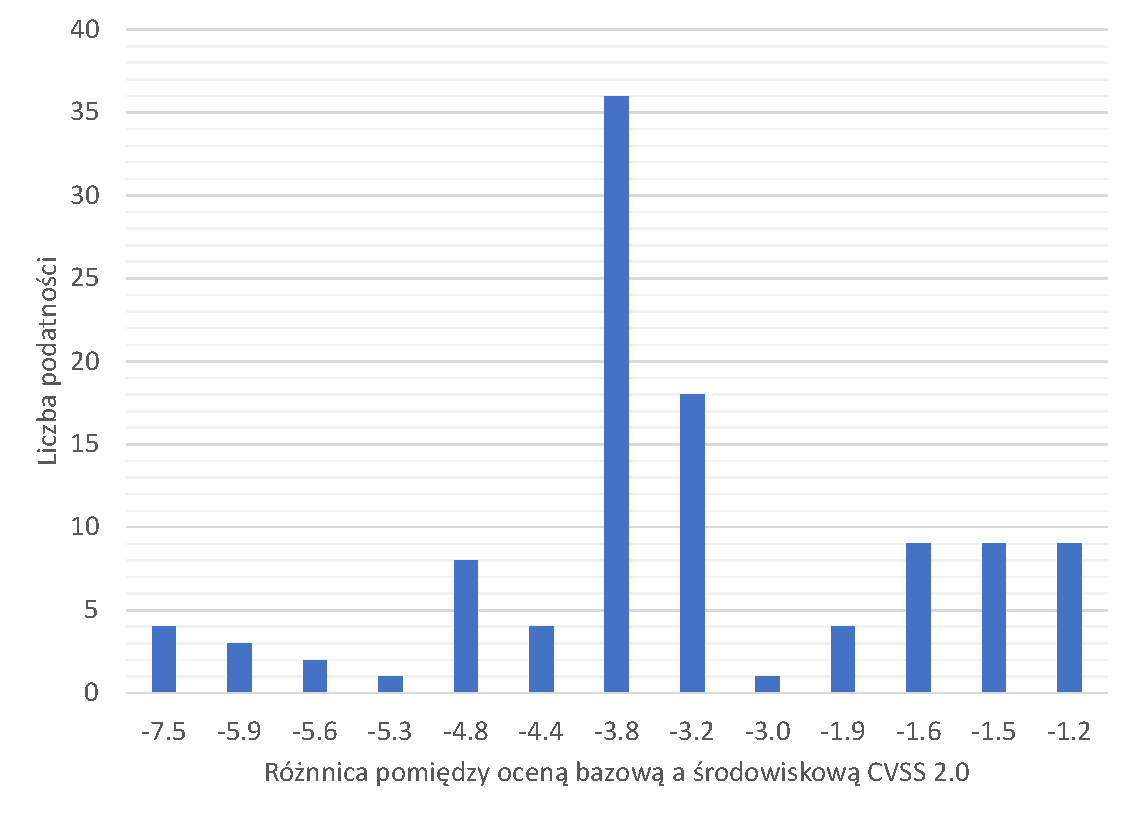
\includegraphics[width=.9\textwidth]{Chapters/Eksperymenty/env_B_results/changes_cvss_2.pdf}
\caption{Liczba podatności zmodyfikowanych dla danej wartości różnicy pomiędzy oceną bazową a środowiskową CVSS 2.0 w przypadku środowiska teleinformatycznego B.}
\label{fig:chapter6:env_b:cvss_2_changes}
\end{figure}

\bigbreak
Tabela \ref{tab:chapter6:env_b:time_results_cvss2} przedstawia liczbę roboczogodzin wymaganą do usunięcia istotnych podatności bezpieczeństwa dla środowiska teleinformatycznego B. W przypadku ocen bazowych CVSS 2.0 szacunkowa liczba roboczogodzin została obliczona za pomocą wzorów: $T_{Base2}$ - \ref{eq:cvss2}, $T_{Base2'}$ - \ref{eq:cvss2prim}. W przypadku oceny środowiskowej CVSS 2.0 szacunkowa liczba roboczogodzin została obliczona za pomocą wzoru \ref{eq:cvss2e}. Wartości dla czasów $T_{Base2}$ obliczone zostały przy założeniu, że administrator musi naprawić tylko podatności o krytyczności wysokiej i średniej, w związku z czym akceptuje ryzyko związane z istnieniem w systemie podatności o krytyczności niskiej. Ponadto należy zauważyć, że w przypadku priortetyzacji opartej na ocenie bazowej CVSS 2.0, która nie uwzględnia danych środowiskowych wśród podatności sklasyfikowanych jako podatności o krytyczności niskiej, mogą się znajdować podatności o wyższej krytyczności, na przykład wysokiej. Wartości czasów $T_{Base2'}$ obliczone zostały zatem przy założeniu, że w celu zapewnienia bezpieczeństwa systemu administrator musi naprawić wszystkie podatności, ponieważ (jak opisano szczegółowo w rozdziale \ref{sec:wplyw_cvss2}) nie ma pewności, czy podatność z otrzymaną oceną bazową CVSS 2.0 zachowa tę ocenę po uwzględnieniu danych środowiskowych. Natomiast wartości dla czasów $T_{Env2}$ obliczone zostały przy założeniu, że wszystkie oceny podatności zostały sklasyfikowane dokładnie (Rozdział \ref{sec:modele-zarzadzaia-podatnosciami}). Gdy porówna się szacowane liczby roboczogodzin otrzymane dla $T_{Base2}$ z $T_{Base2'}$, można zauważyć wzrost szacowanej liczby roboczogodzin dla wszystkich rozpatrywanych przypadków ($T_{FIX_{MIN}}$, $T_{FIX_{AVERAGE}}$, $T_{FIX_{MAX}}$), który wynosi 3.6\%. Ponadto można zaobserwować, że naprawienie wszystkich podatności według otrzymanej priorytetyzacji za pomocą oceny bazowej CVSS 2.0 redukuje ryzyko nienaprawienia podatności niedoszacowanej z 3.8\% do 0\%. Gdy porównamy otrzymane wyniki dla $T_{Base2}$ i $T_{Env2}$, można zauważyć, że średni zysk w postaci obniżenia szacowanej liczby roboczogodzin dla wszystkich rozpatrywanych przypadków wynosi 75\%. Wykorzystanie priorytetyzacji za pomocą oceny środowiskowej CVSS 2.0 pozwala na obniżenie ryzyka związanego z nienaprawieniem podatności niedoszacowanej z 3.8\% do 0\%. Natomiast gdy porówna się wyniki otrzymane dla $T_{Base2'}$ i $T_{Env2}$, można zauważyć, że średni zysk w postaci obniżenia szacowanej liczby roboczogodzin dla wszystkich rozpatrywanych przypadków wynosi 75.9\% i tym samym utrzymuje ryzyko związane z nienaprawieniem podatności niedoszacowanych na poziomie 0\%.

\begin{table}[tbh]
\caption{Liczba roboczogodzin wymagana do usunięcia podatności bezpieczeństwa dla środowiska teleinformatycznego B. W przypadku ocen bazowych CVSS 2.0 szacunkowa liczba roboczogodzin została obliczona za pomocą wzorów: $T_{Base2}$ - \ref{eq:cvss2}, $T_{Base2'}$ - \ref{eq:cvss2prim}. W przypadku oceny środowiskowej CVSS 2.0 szacunkowa liczba roboczogodzin została obliczona za pomocą wzoru \ref{eq:cvss2e}.}
\begin{center}
\label{tab:chapter6:env_b:time_results_cvss2}
\begin{tabular}{c|ccc|c}
\hline
                 & \textbf{$T_{FIX_{MIN}}$} & \textbf{$T_{FIX_{AVERAGE}}$} & \textbf{$T_{FIX_{MAX}}$ }  & Średnia \% zmiana \\
\hline
$T_{Base2}$      &                        119h &              469h &    919h         &        \\
$T_{Base2'}$     &                        123h &              486h &    955h         &         \\
Różnica          &                +4h (+3.4\%) &       +17h (+3.6\%) & +36h (+3.9\%) & +3.6\%   \\  
\hline
$T_{Base2}$      &                       119h &              469h &    919h         &         \\
$T_{Env2}$       &                        38h &            104.5h &    190h         &         \\
Różnica          &             -81h (-68\%) & -364.5h (-77.7\%) & -729h (-79.3\%) & -75\% \\  
\hline
$T_{Base2'}$     &                       123h &              486h &     955h        &         \\
$T_{Env2}$        &                       38h &            104.5h &     190h        &         \\
Różnica          &             -85h (-69.1\%) & -381.5h (-78.5\%) & -765h (-80.1\%) & -75.9\% \\  
\hline
\end{tabular}
\end{center}
\end{table}

\bigbreak
Jak wykazano w przeprowadzonej analizie, model zarządzania podatnościami, który wykorzystuje ocenę środowiskową CVSS 2.0, ma istotną wadę. Wada ta polega na tym, że parametr $TD$, który służy do ustalania liczby systemów wrażliwych na daną podatność, znacząco zaniża oceny wszystkich wykrytych podatności. W analizowanym środowisku teleinformatycznym B spowodował sklasyfikowanie znacznej większości podatności do kategorii niskiej. Dlatego też ocena środowiskowa CVSS 2.0 nie jest dokładną miarą bezpieczeństwa infrastruktury teleinformatycznej. Analiza wyników pozwala na wyciągnięcie kolejnego wniosku. Mianowicie model zarządzania podatnościami przy zastosowaniu oceny środowiskowej CVSS 2.0 (Rysunek \ref{fig:chapter1:vm-model-cvss2e}) może być wykorzystany do wykrywania podatności, które mogą zagrozić większej liczbie skanowanych zasobów. Taka informacja jest niezwykle cenna dla wszystkich osób zaangażowanych w proces zarządzania podatnościami (Rozdział \ref{sec:proces-zarzadzania-podatnosciami}), ponieważ pozwala na podjęcie szybkiej decyzji dotyczącej naprawy podatności oraz skrócenie czasu ich obecności w monitorowanej infrastrukturze teleinformatycznej.

%%%%%%%%%%%%%%%%%%%%%%%%%%%%%%%%%%%%%%%%%%%%%%%%

%%%%%%%%%%%%%%%%%%%%%%%%%%%%%%%%%%%%%%%%%%%%%%%%
\subsubsection{Analiza wpływu parametrów środowiskowych na ocenę bazową CVSS 3.x}

Rysunek \ref{fig:chapter6:env_b:cvss_3} przedstawia liczbę wykrytych podatności dla każdej kategorii krytyczności według oceny bazowej i środowiskowej CVSS 3.x dla środowiska teleinformatycznego B. Na podstawie wyników pokazanych na rysunku \ref{fig:chapter6:env_b:cvss_3} można stwierdzić, że dla oceny środowiskowej CVSS 3.x wszystkie podatności nie zmieniły kategorii krytyczności. Wpływ na to ma brak informacji od administratora środowiska teleinformatycznego B na temat parametrów środowiskowych $CIA$. W rezultacie bez dostarczonych informacji od administratora środowiska teleinformatycznego B, niemożliwe było wykonanie ponownej priorytetyzacji oraz oszacowanie zysków z wykorzystania modelu zarządzania podatnościami opartego o ocenę środowiskową CVSS 3.x (Rysunek \ref{eq:cvss2e}). Wyniki przedstawione na rysunkach \ref{fig:chapter6:env_a:cvss_3} oraz \ref{fig:chapter6:env_b:cvss_3} pokazują jak ważne jest posiadanie zbudowanej bazy inwentaryzacyjnej z określonymi wagami zasobów teleinformatycznych pod kątem wymagań ciągłości, integralności oraz dostępności w procesie zarządzania podatnościami.


\begin{figure}[!ht]
\centering
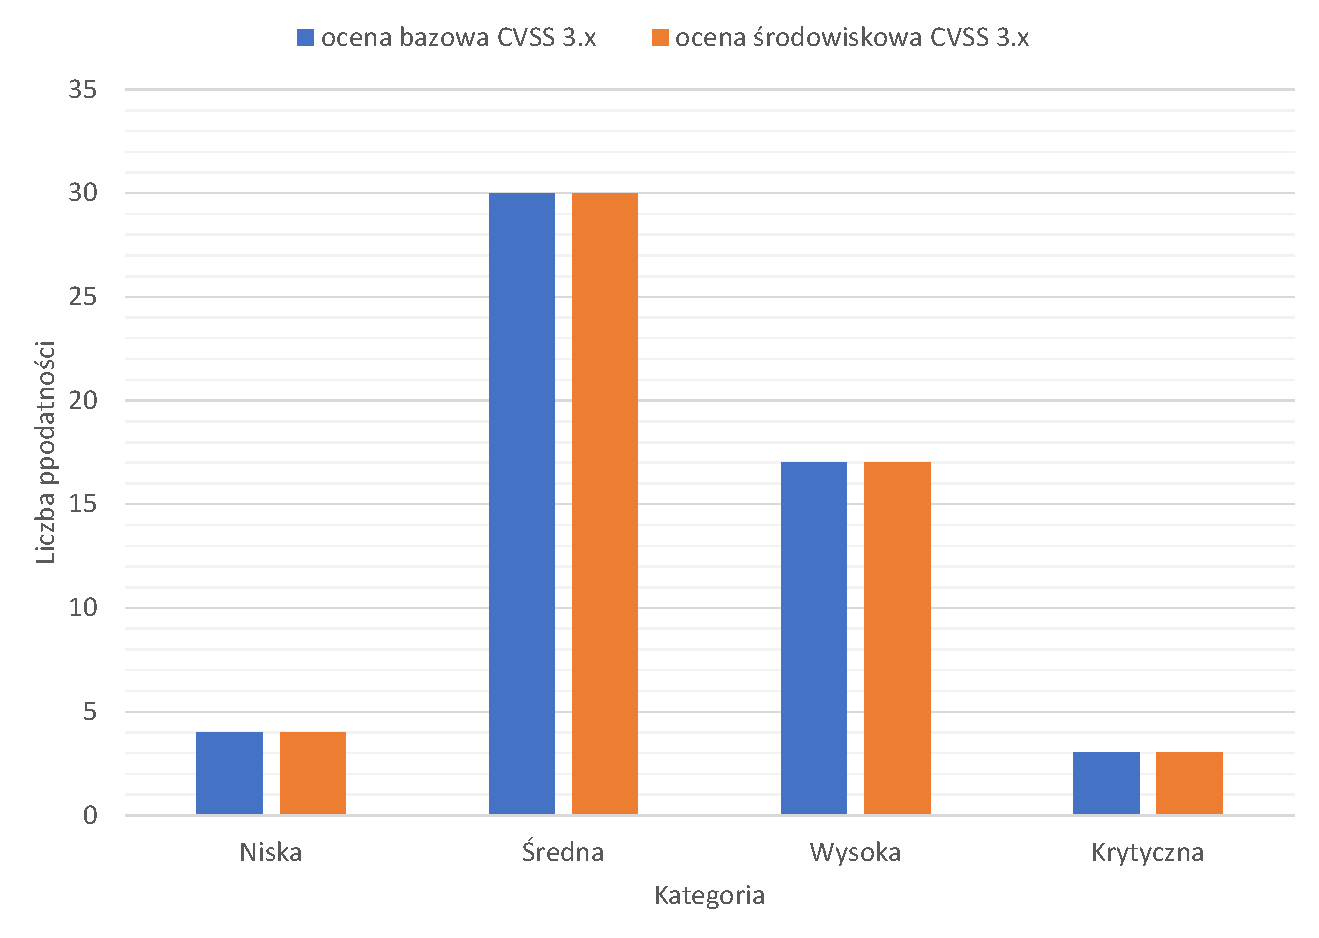
\includegraphics[width=.9\textwidth]{Chapters/Eksperymenty/env_B_results/cvss_3.pdf}
\caption{Liczba wykrytych podatności dla każdej kategorii krytyczności według oceny bazowej i środowiskowej CVSS 3.x dla środowiska teleinformatycznego B.}
\label{fig:chapter6:env_b:cvss_3}
\end{figure}

%%%%%%%%%%%%%%%%%%%%%%%%%%%%%%%%%%%%%%%%%%%%%%%%

%%%%%%%%%%%%%%%%%%%%%%%%%%%%%%%%%%%%%%%%%%%%%%%%

\subsubsection{Podsumowanie wyników analizy dla środowiska B}
Na podstawie wyników przedstawionych w podrozdziale ''Analiza wpływu parametrów środowiskowych na ocenę bazową CVSS 2.0' można stwierdzić, że dla oceny środowiskowej znacząca większość podatności zostały przydzielone do kategorii niskiej. Wpływ na to ma parametr $TD$, który osiągnął maksymalną wartość 25\%. Otrzymana maksymalna wartość oznacza, że w środowisku teleinformatycznym B wykryte zostały podatności, na które wrażliwe jest 9 skanowanych zasobów. Dlatego też wszystkie podatności, dla których parametr $TD$ ma wartość 25\%, zostały przydzielone do kategorii średniej. Dodatkowo z analizy otrzymanych wyników można stwierdzić, że dodanie do oceny bazowej CVSS 2.0 danych środowiskowych powoduje znaczącą redukcję szacowanej liczby roboczogodzin wymaganą do usunięcia istotnych podatności wykrytych w środowisku teleinformatycznym B. Gdy porównamy wyniki otrzymane dla oceny bazowej CVSS 2.0 ($T_{Base2}$) z oceną środowiskową CVSS 2.0 ($T_{Env2}$), można zauważyć, że średni zysk w postaci obniżenia szacowanej liczby roboczogodzin wynosi 75.9\%. Wykorzystanie priorytetyzacji za pomocą oceny środowiskowej CVSS 2.0 pozwala na obniżenie ryzyka związanego z nienaprawieniem podatności niedoszacowanej z 3.8\% do 0\%. Wyniki przedstawione w podrozdziale ''Analiza wpływu parametrów środowiskowych na ocenę bazową CVSS 2.0'' potwierdzają wadę oceny środowiskowej CVSS 2.0 polegającą na tym, że parametr $TD$, który służy do ustalania liczby systemów wrażliwych na daną podatność, znacząco zaniża oceny wszystkich podatności. Pomimo wspomnianej wady, na podstawie otrzymanych wyników, można dodatkowo stwierdzić, że wartość parametru $TD$ może być wykorzystana do wykrywania podatności, które mogą zagrozić większej liczbie skanowanych zasobów. Ponieważ jednak parametr $TD$ zaniża oceny wszystkich podatności, konieczne było rozważenie modelu zarządzania podatnościami, który opiera się na standardzie CVSS 3.x.

\bigbreak
Na podstawie wyników przedstawionych w podrozdziale ''Analiza wpływu parametrów środowiskowych na ocenę bazową CVSS 3.x'' można stwierdzić, że dla oceny środowiskowej CVSS 3.x wszystkie podatności nie zmieniły kategorii krytyczności. Wpływ na to ma brak dostarczonych informacji od administratora środowiska teleinformatycznego B na temat parametrów środowiskowych $CIA$. Z otrzymanych wyników można stwierdzić, że bez określonych parametrów środowiskowych $CIA$ niemożliwe jest wykonanie ponownej priorytetyzacji podatności dla modelu zarządzania podatnościami opartego o ocenę środowiskową CVSS 3.x (Rysunek \ref{fig:chapter1:vm-model-cvss3e}). W rezultacie na podstawie otrzymanych wyników można stwierdzić, że potwierdzają wniosek dotyczący istotności posiadania zbudowanej bazy zasobów, w której określone zostaną parametry $CIA$ dla każdego z monitorowanych zasobów.


%%%%%%%%%%%%%%%%%%%%%%%%%%%%%%%%%%%%%%%%%%%%%%%%

%%%%%%%%%%%%%%%%%%%%%%%%%%%%%%%%%%%%%%%%%%%%%%%%
\subsection{Analiza dla środowiska teleinformatycznego C}


%%%%%%%%%%%%%%%%%%%%%%%%%%%%%%%%%%%%%%%%%%%%%%%%

%%%%%%%%%%%%%%%%%%%%%%%%%%%%%%%%%%%%%%%%%%%%%%%%
\subsubsection{Analiza wpływu parametrów środowiskowych na ocenę bazową CVSS 2.0}
Rysunek \ref{fig:chapter6:env_c:cvss_2} przedstawia liczbę wykrytych podatności dla każdej kategorii krytyczności według oceny bazowej i środowiskowej CVSS 2.0. Na podstawie wyników pokazanych na rysunku \ref{fig:chapter6:env_c:cvss_2} można stwierdzić, że dla oceny środowiskowej CVSS 2.0 wszystkie podatności zostały przydzielone do kategorii niskiej. Wpływ na to ma parametr $TD$ (Rozdział \ref{sec:td}), który osiągnął maksymalną wartość 3\%, co zostało przedstawione na rysunku \ref{fig:chapter6:env_c:cvss_2_td}. Parametr $TD$ wskazuje procent zasobów wrażliwych na konkretną podatność. Rysunek \ref{fig:chapter6:env_c:cvss_2_td} przedstawia wartość parametru $TD$ dla wykrytych podatności w środowisku teleinformatycznym C. Wpływ pozostałych parametrów środowiskowych na kategorię krytyczności podatności, $CDP$ (Rozdział \ref{sec:cdp}) oraz $CIA$ (Rozdział \ref{sec:cia_desc}) jest niezauważalny, ponieważ parametr $TD$ osiąga maksymalną wartość 3\%. Wyniki przedstawione na rysunku \ref{fig:chapter6:env_c:cvss_2} potwierdzają, że model zarządzania podatnościami, który wykorzystuje ocenę środowiskową CVSS 2.0, ma istotną wadę. Wada ta polega na tym, że parametr $TD$, który służy do ustalania liczby systemów wrażliwych na daną podatność, znacząco zaniża oceny wszystkich podatności. Dlatego też model zarządzania podatnościami oparty o ocenę środowiskową CVSS 2.0 nie jest dokładną miarą bezpieczeństwa infrastruktury teleinformatycznej. Konieczne jest zatem rozważenie modelu zarządzania podatnościami, który opiera się na standardzie CVSS 3.x. Niemniej jednak należy zauważyć, że ocena środowiskowa CVSS 2.0 dostarcza bardzo ważnej informacji dla administratora. Mianowicie jeśli wartość parametru $TD$ jest niska, to w badanym środowisku teleinformatycznym wykryta podatność może zagrozić jedynie niewielkiej liczbie serwerów. Na przykład w środowisku C wykryto podatności, których wykorzystanie możne zagrozić co najwyżej 62 serwerom, tj. 3\% skanowanych zasobów.

\begin{figure}[!ht]
\centering
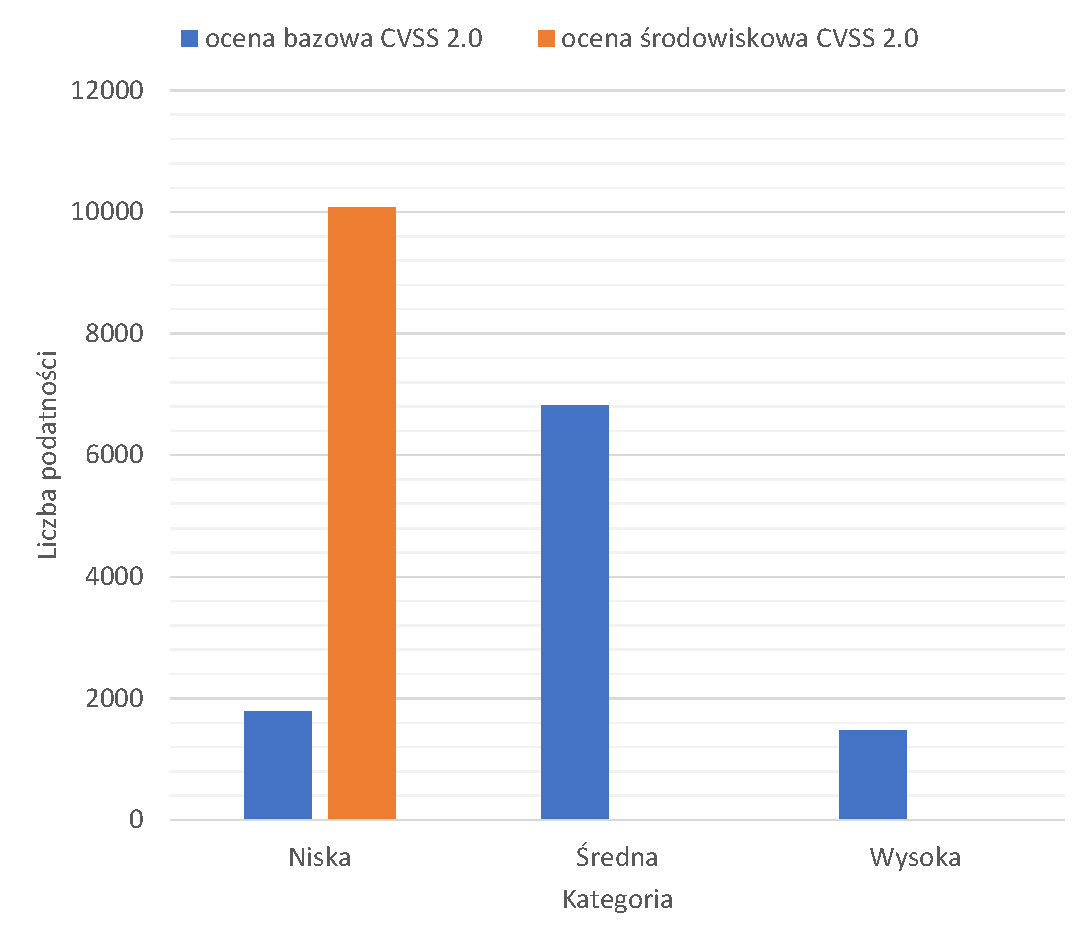
\includegraphics[width=.9\textwidth]{Chapters/Eksperymenty/env_C_results/cvss_2.pdf}
\caption{Liczba wykrytych podatności dla każdej kategorii krytyczności według oceny bazowej i środowiskowej CVSS 2.0 dla środowiska teleinformatycznego C.}
\label{fig:chapter6:env_c:cvss_2}
\end{figure}

\begin{figure}[!ht]
\centering
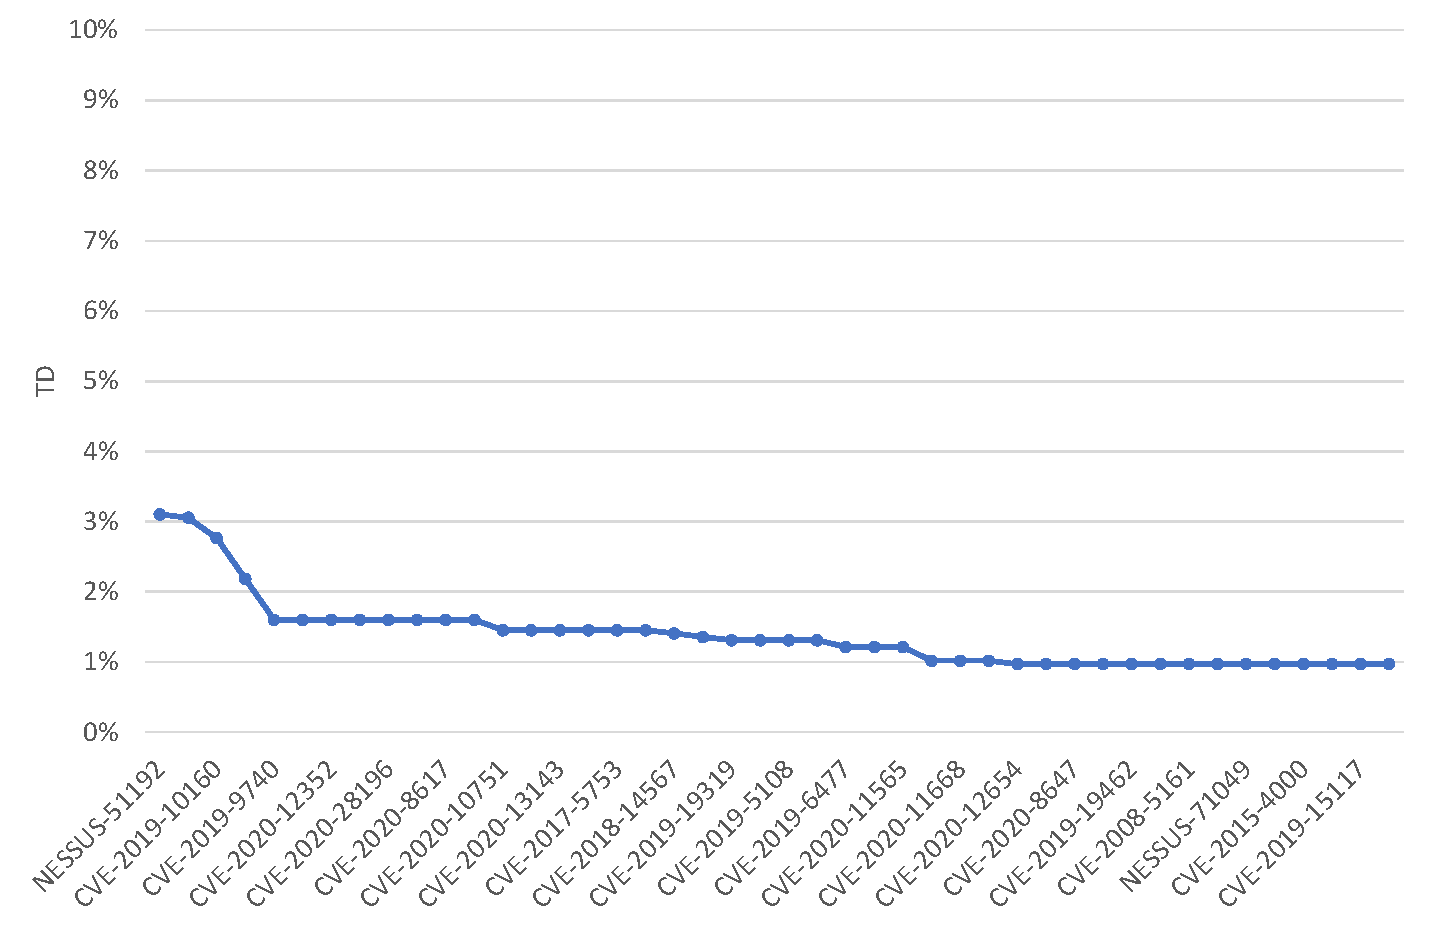
\includegraphics[width=.9\textwidth]{Chapters/Eksperymenty/env_C_results/cvss_2_td_env_c.pdf}
\caption{Wartość parametru $TD$ dla wykrytych podatności w środowisku teleinformatycznym C.}
\label{fig:chapter6:env_c:cvss_2_td}
\end{figure}

\bigbreak
Rysunek \ref{fig:chapter6:env_c:cvss_2_changes} przedstawia liczbę podatności zmodyfikowanych dla danej wartości różnicy pomiędzy oceną bazową a środowiskową CVSS 2.0 w przypadku środowiska teleinformatycznego C. Uwzględnienie parametrów środowiskowych $CIA$, $CDP$, $TD$ spowodowało zmianę wszystkich ocen bazowych CVSS 2.0 w przedziale od -10.0 do -1.2. Brak ocen bazowych niezmodyfikowanych spowodowany jest postacią równania \ref{eq:cvss2_es}, w którym to występuje mnożenie oceny końcowej przez wartość parametru środowiskowego $TD$ w celu otrzymania wartości oceny środowiskowej CVSS 2.0. Z liczby oraz zakresu zmian można wywnioskować, że w zbiorze wykrytych podatności znajdują się zagrożenia, które mogą mieć istotny wpływ na bezpieczeństwo monitorowanego środowiska. 

Zbiór wykrytych podatności w środowisku teleinformatycznym C składa się z dwóch podzbiorów: podatności posiadających obie oceny bazowe (CVSS 2.0 oraz CVSS 3.x) oraz podatności ze znaną jedynie oceną bazową w standardzie CVSS 2.0. W przypadku pierwszego podzbioru podatności posiadają ocenę bazową według standardu CVSS 3.x, w związku z czym priorytetyzacja naprawy zostanie ujęta w procesie zarządzania podatnościami za pomocą modelu \ref{fig:chapter1:vm-model-cvss3e} (Rozdział \ref{sec:proces-zarzadzania-podatnosciami}), ponieważ stosowanie oceny bazowej CVSS 3.x pozwala dokładniej ocenić krytyczność podatności, a zatem skuteczniej oszacować zagrożenia (Rozdział \ref{sec:modele-zarzadzaia-podatnosciami}). W przypadku drugiego podzbioru, który zawiera 348 (3.45\%) podatności, wykorzystano mechanizm konwersji oceny bazowej CVSS 2.0 do 3.x opisany w rozdziale \ref{sec:ml} w celu umożliwienia wykonania priorytetyzacji za pomocą modelu oceny środowiskowej CVSS 3.x (Rysunek \ref{fig:chapter1:vm-model-cvss3e}). 

\begin{figure}[!ht]
\centering
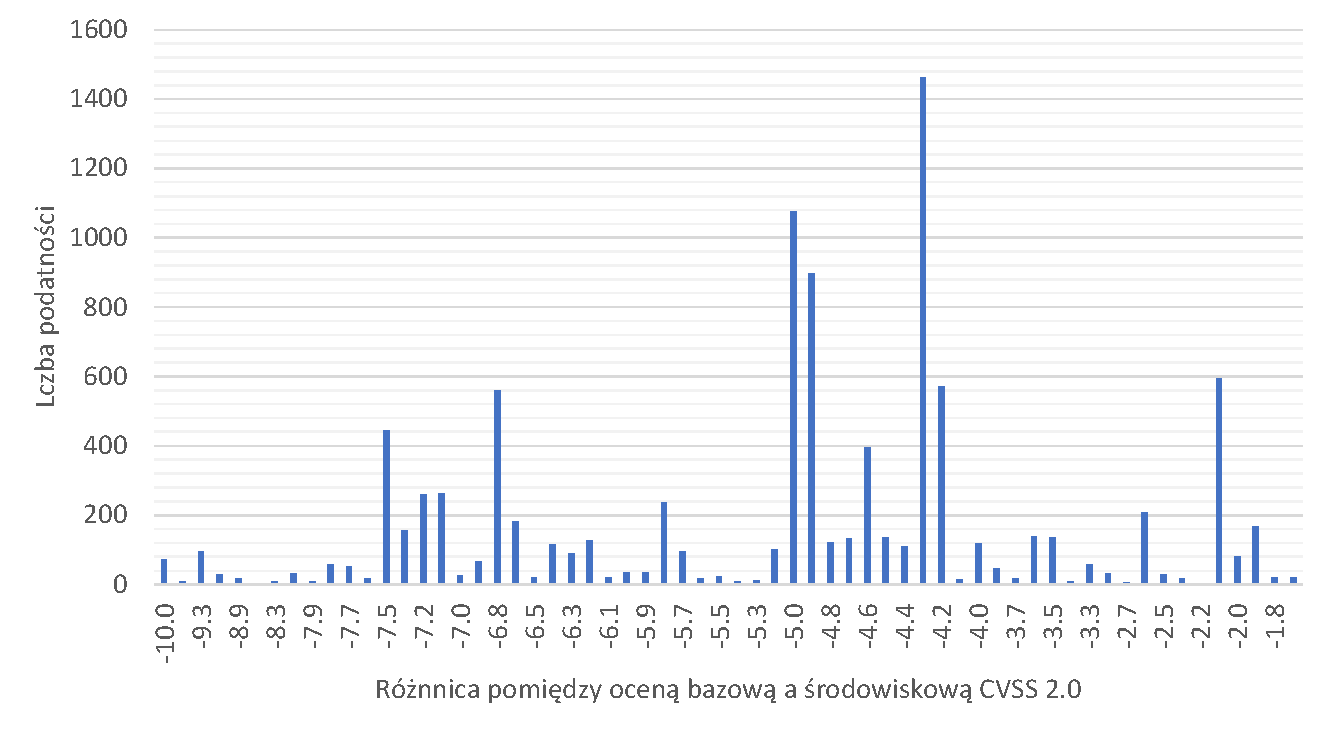
\includegraphics[width=.9\textwidth]{Chapters/Eksperymenty/env_C_results/changes_cvss_2.pdf}
\caption{Liczba podatności zmodyfikowanych dla danej wartości różnicy pomiędzy oceną bazową a środowiskową CVSS 2.0 w przypadku środowiska teleinformatycznego C.}
\label{fig:chapter6:env_c:cvss_2_changes}
\end{figure}

\bigbreak
Tabela \ref{tab:chapter6:env_c:time_results_cvss2} przedstawia liczbę roboczogodzin wymaganą do usunięcia istotnych podatności bezpieczeństwa dla środowiska teleinformatycznego C. W przypadku ocen bazowych CVSS 2.0 szacunkowa liczba roboczogodzin została obliczona za pomocą wzorów: $T_{Base2}$ - \ref{eq:cvss2}, $T_{Base2'}$ - \ref{eq:cvss2prim}. W przypadku oceny środowiskowej CVSS 2.0 szacunkowa liczba roboczogodzin została obliczona za pomocą wzoru \ref{eq:cvss2e}. Wartości dla czasów $T_{Base2}$ obliczone zostały przy założeniu, że administrator musi naprawić tylko podatności o krytyczności wysokiej i średniej, w związku z czym akceptuje ryzyko związane z istnieniem w systemie podatności o krytyczności niskiej. Ponadto należy zauważyć, ze w przypadku priortetyzacji opartej na ocenie bazowej CVSS 2.0, która nie uwzględnia danych środowiskowych wśród podatności sklasyfikowanych jako podatności o krytyczności niskiej, mogą się znajdować podatności o wyższej krytyczności, na przykład wysokiej. Wartości czasów $T_{Base2'}$ obliczone zostały zatem przy założeniu, że w celu zapewnienia bezpieczeństwa systemu administrator musi naprawić wszystkie podatności, ponieważ (jak opisano szczegółowo w rozdziale \ref{sec:wplyw_cvss2}) nie ma pewności czy podatność z otrzymaną oceną bazową CVSS 2.0 zachowa tę ocenę po uwzględnieniu danych środowiskowych. Natomiast wartości dla czasów $T_{Env2}$ obliczone zostały przy założeniu, że wszystkie oceny podatności zostały sklasyfikowane dokładnie (Rozdział \ref{sec:modele-zarzadzaia-podatnosciami}). Gdy porówna się szacowane liczby roboczogodzin otrzymane dla $T_{Base2}$ z $T_{Base2'}$, można zauważyć wzrost szacowanej liczy roboczogodzin dla wszystkich rozpatrywanych przypadków ($T_{FIX_{MIN}}$, $T_{FIX_{AVERAGE}}$, $T_{FIX_{MAX}}$), który wynosi 16.7\%. Ponadto można zaobserwować, że naprawienie wszystkich podatności według otrzymanej priorytetyzacji za pomocą oceny bazowej CVSS 2.0 redukuje ryzyko nienaprawienia podatności niedoszacowanej z 17.8\% do 0\%. Gdy porównamy otrzymane wyniki dla $T_{Base2}$ i $T_{Env2}$, można zauważyć, że średni zysk w postaci obniżenia szacowanej liczby roboczogodzin dla wszystkich rozpatrywanych przypadków wynosi 99.8\%. Wykorzystanie priorytetyzacji za pomocą oceny środowiskowej CVSS 2.0 pozwala na obniżenie ryzyka związanego z nienaprawieniem podatności niedoszacowanej z 17.8\% do 0\%. Natomiast gdy porówna się wyniki otrzymane dla $T_{Base2'}$ i $T_{Env2}$, można zauważyć, że średni zysk w postaci obniżenia szacowanej liczby roboczogodzin dla wszystkich rozpatrywanych przypadków wynosi 99.9\% i tym samym utrzymuje ryzyko związane z nienaprawieniem podatności niedoszacowanych na poziomie 0\%.

\begin{table}[tbh]
\caption{Liczba roboczogodzin wymagana do usunięcia istotnych podatności dla bezpieczeństwa środowiska teleinformatycznego C. W przypadku ocen bazowych CVSS 2.0 szacunkowa liczba roboczogodzin została obliczona za pomocą wzorów: $T_{Base2}$ - \ref{eq:cvss2}, $T_{Base2'}$ - \ref{eq:cvss2prim}. W przypadku oceny środowiskowej CVSS 2.0 szacunkowa liczba roboczogodzin została obliczona za pomocą wzoru \ref{eq:cvss2e}.}
\begin{center}
\label{tab:chapter6:env_c:time_results_cvss2}
\begin{tabular}{c|ccc|c}
\hline
                 & \textbf{$T_{FIX_{MIN}}$} & \textbf{$T_{FIX_{AVERAGE}}$} & \textbf{$T_{FIX_{MAX}}$ }  & Średnia \% zmiana \\
\hline
$T_{Base2}$      &                      8 311h &         37 319h   &  74 615h           &        \\
$T_{Base2'}$     &                     10 101h &         45 374h   &  90 725h           &         \\
Różnica          &           +1 790h (+21.5\%) & +8 055h (+21.6\%) & +16 110h (+21.6\%) & +21.6\%   \\  
\hline
$T_{Base2}$     &                       8 311h &           37 319h &  74 615h        &         \\
$T_{Env2}$        &                        23h &               23h &     23h         &         \\
Różnica          &           -8 288h (-99.7\%) & -37 269h (-99.9\%) & -74 592h (-99.9\%) & -99.8\% \\  
\hline
$T_{Base2'}$     &                      10 101h &       45 374h    &  90 725h        &         \\
$T_{Env2}$        &                        23h &               23h  &     23h        &         \\
Różnica          &           -10 078h (-99.8\%) & -45 351h (-99.9\%) & -90 702h (-99.9\%) & -99.9\% \\  
\hline
\end{tabular}
\end{center}
\end{table}

\bigbreak
Jak wykazano w przeprowadzonej analizie, model zarządzania podatnościami, który wykorzystuje ocenę środowiskową CVSS 2.0, ma istotną wadę. Wada ta polega na tym, że parametr $TD$, który służy do ustalania liczby systemów wrażliwych na daną podatność, znacząco zaniża oceny wszystkich wykrytych podatności. W analizowanym środowisku teleinformatycznym C spowodował sklasyfikowanie wszystkich podatności do kategorii niskiej. Dlatego też ocena środowiskowa CVSS 2.0 nie jest dokładną miarą bezpieczeństwa infrastruktury teleinformatycznej. Analiza wyników pozwala na wyciągnięcie kolejnego wniosku. Mianowicie model zarządzania podatnościami przy zastosowaniu oceny środowiskowej CVSS 2.0 (Rysunek \ref{fig:chapter1:vm-model-cvss2e}) może być wykorzystany do wykrywania podatności, które mogą zagrozić większej liczbie skanowanych zasobów. Taka informacja jest niezwykle cenna dla wszystkich osób zaangażowanych w proces zarządzania podatnościami (Rozdział \ref{sec:proces-zarzadzania-podatnosciami}), ponieważ pozwala na podjęcie szybkiej decyzji dotyczącej naprawy podatności oraz skrócenie czasu ich obecności w monitorowanej infrastrukturze teleinformatycznej.

%%%%%%%%%%%%%%%%%%%%%%%%%%%%%%%%%%%%%%%%%%%%%%%%

%%%%%%%%%%%%%%%%%%%%%%%%%%%%%%%%%%%%%%%%%%%%%%%%
\subsubsection{Analiza wpływu parametrów środowiskowych na ocenę bazową CVSS 3.x}

W celu wykonania analizy wpływu parametrów środowiskowych na ocenę bazową CVSS 3.x rozróżniono dwa przypadki. W pierwszym przypadku rozważane jest wykorzystanie metody konwersji ocen bazowych CVSS 2.0 do 3.x za pomocą uczenia maszynowego. W drugim przypadku rozważane jest brak metod konwersji i dopuszczany jest brak wiedzy na temat wszystkich ocen bazowych CVSS 3.x dla nieznacznej liczby wykrytych podatności.

\bigbreak
Dla pierwszego rozpatrywanego przypadku, w celu zapewnienia poprawnej priorytetyzacji wszystkich podatności za pomocą modeli zarządzania podatnościami wykorzystującymi CVSS 3.x (Rysunki \ref{fig:chapter1:vm-model-cvss3}, \ref{fig:chapter1:vm-model-cvss3e}), wykorzystano mechanizm konwersji CVSS 2.0 do CVSS 3.x za pomocą uczenia maszynowego (Rozdział \ref{sec:ml}, ponieważ 34\% podatności nie posiada oceny bazowej według CVSS 3.x dla środowiska teleinformatycznego C (Rozdział \ref{sec:desc_c}). W tabeli \ref{tab:chapter6:env_c:ml_classification} przedstawiono liczbę zmian dla każdej kategorii podatności według oceny bazowej CVSS 3.x w przypadku środowiska teleinformatycznego C, po zastosowaniu mechanizmu konwersji oceny bazowej CVSS 2.0 do CVSS 3.x (ML) opartego na uczeniu maszynowym. Wykorzystany mechanizm uczenia maszynowego oblicza ocenę bazową CVSS 3.x obarczoną błędem klasyfikacji kategorii krytyczności wynoszącym 3.45\%, co oznacza, że można oczekiwać 48 podatności błędnie sklasyfikowanych w środowisku teleinformatycznym C. W dalszej części podrozdziału skupiono się tylko na analizie wyników przypadku pierwszego dotyczącego prioretetyzacji podatności według oceny środowiskowej CVSS 3.x z wykorzystaniem metod konwersji ocen bazowych CVSS 2.0 do 3.x za pomocą uczenia maszynowego.


\begin{table}[tbh]
\caption{Liczba zmian dla każdej kategorii podatności według oceny bazowej CVSS 3.x w przypadku środowiska teleinformatycznego C po zastosowaniu mechanizmu konwersji oceny bazowej CVSS 2.0 do CVSS 3.x (ML) opartego na uczeniu maszynowym.}
\begin{center}
\label{tab:chapter6:env_c:ml_classification}
\begin{tabular}{cccc}
\hline \noalign {\smallskip}
\textbf{Kategoria} & \textbf{ocena bazowa} & \textbf{[ML] ocena bazowa} & \textbf{Różnica} \\
                      & \textbf{CVSS 3.x} & \textbf{CVSS 3.x} & \\
  \hline
  Niska         &    802 &  996    &  +194          \\
                &        &         &  (+24.1\%)     \\
  Średnia       &  4 453 &   4 511 &  +58           \\
                &        &         &  (+1.3\%)       \\
  Wysoka        &  2 651 &   2 682 &  +31           \\
                &        &         &  (+1.2\%)   \\
  Krytyczna     &  1 824 &  1 889  &  +65          \\
                &        &         &  (+3.6\%)   \\
\hline \noalign {\smallskip}
\textbf{Razem}  &   9 730 &   10 078& +348 \\
                &        &         & (+3.6\%) \\
\hline \noalign {\smallskip}
\end{tabular}
\end{center}
\end{table}

\bigbreak
Rysunek \ref{fig:chapter6:env_c:cvss_3} przedstawia liczbę wykrytych podatności dla każdej kategorii krytyczności według oceny bazowej i środowiskowej CVSS 3.x dla środowiska teleinformatycznego C. Na podstawie wyników pokazanych na rysunku \ref{fig:chapter6:env_a:cvss_3} można stwierdzić znaczącą zmianę w stosunku do oceny bazowej CVSS 3.x, która polega na zmniejszeniu liczby podatności krytycznych oraz wysokich a zwiększeniu liczby podatności o kategorii średniej oraz niskiej. Wpływ na to mają ustawienia wagi zasobów, wskazane przez administratora środowiska teleinformatycznego C o rozkładzie przedstawionym na rysunku \ref{fig:chapter5:env_c:os_cia}. Analiza wpływu parametrów środowiskowych $CIA$ na ocenę bazową CVSS 3.x przedstawiona została w rozdziale 4.

\begin{figure}[!ht]
\centering
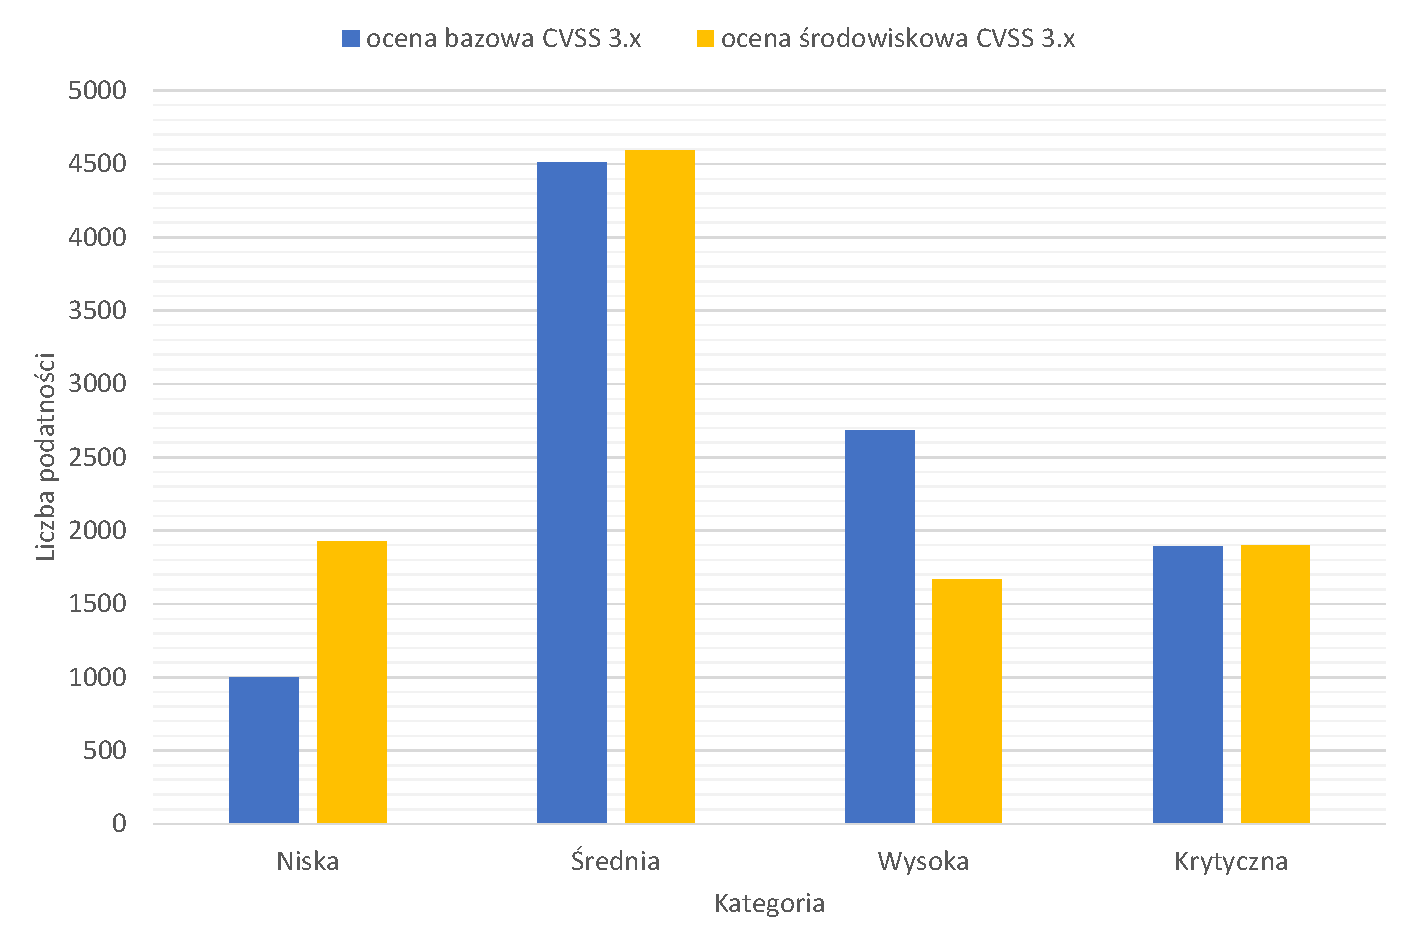
\includegraphics[width=.9\textwidth]{Chapters/Eksperymenty/env_C_results/cvss_3_ml.pdf}
\caption{Liczba wykrytych podatności dla każdej kategorii krytyczności według oceny bazowej i środowiskowej CVSS 3.x dla środowiska teleinformatycznego C.}
\label{fig:chapter6:env_c:cvss_3}
\end{figure}

\bigbreak
Rysunek \ref{fig:chapter6:env_c:cvss_3_changes} przedstawia liczbę wszystkich podatności zmodyfikowanych dla danej wartości różnicy pomiędzy oceną bazową a środowiskową CVSS 3.x w przypadku środowiska teleinformatycznego C. Wyniki przedstawione na rysunku \ref{fig:chapter6:env_c:cvss_3_changes} dotyczą rozpatrywanego przypadku pierwszego, w którym to uwzględnione są podatności z obliczoną oceną bazową CVSS 3.x za pomocą uczenia maszynowego. Parametry środowiskowe $CIA$ dla wskazanych zasobów spowodowały modyfikację  6 121 (60.73\%) ocen bazowych w zakresie od -2.3 do 2.2. Na pozostałe podatności ustawienia parametrów środowiskowych nie miały wpływu.

\begin{figure}[!ht]
\centering
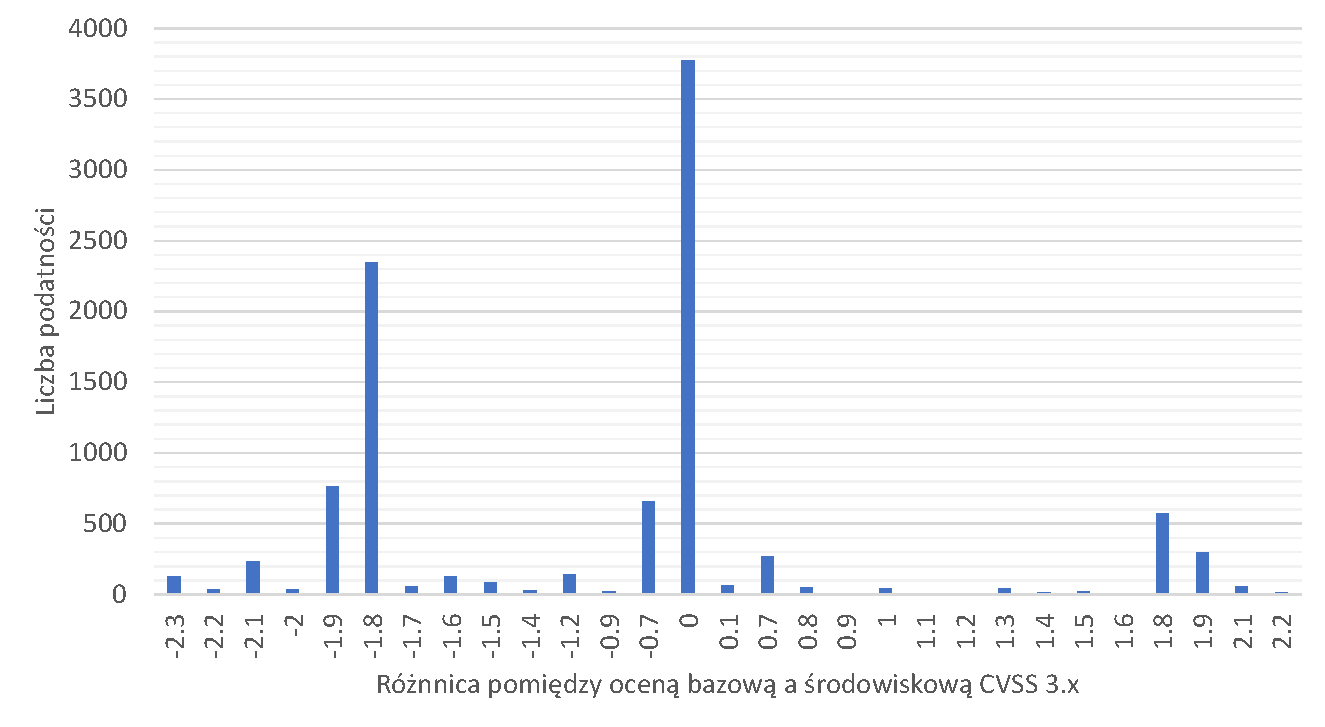
\includegraphics[width=.9\textwidth]{Chapters/Eksperymenty/env_C_results/changes_cvss_3.pdf}
\caption{Liczba wszystkich podatności zmodyfikowanych dla danej wartości różnicy pomiędzy oceną bazową a środowiskową CVSS 3.x w przypadku środowiska teleinformatycznego C.}
\label{fig:chapter6:env_c:cvss_3_changes}
\end{figure}

\bigbreak
Tabela \ref{tab:chapter6:env_c:changes_cvss_3} przedstawia liczbę zmian w kategoriach krytyczności podatności dla środowiska teleinformatycznego C po uwzględnieniu parametrów środowiskowych $CIA$ przy wykorzystaniu metod konwersji oceny bazowej CVSS 2.0 do 3.x za pomocą uczenia maszynowego. Największa zmiana w liczbie podatności została odnotowana dla kategorii krytycznej (+94.58\%) oraz wysokiej (-39.96\%). Dla zasobów posiadających wartości parametrów środowiskowych $CIA$ wykryto 10 023 podatności, co stanowi 99.45\% wszystkich podatności, 21.98\% z nich zmieniło swoją kategorię. Uzyskane wyniki pozwalają na wyciągnięcie dwóch wniosków. Pierwszy mówi o tym, że możliwe jest wykorzystanie mechanizmu konwersji oceny bazowej CVSS 2.0 do 3.x do pełnej implementacji modelu zarządzania podatnościami opartego na ocenie środowiskowej CVSS 3.x dla wszystkich podatności. Natomiast drugi wniosek pozwala na stwierdzenie, że każda dodatkowa informacja na temat monitorowanego środowiska wpływa na priorytetyzacje napraw podatności poprzez możliwość zmiany kategorii krytyczności podatności.

\begin{table}[tbh]
\caption{Liczba zmian w kategoriach podatności dla środowiska teleinformatycznego C z wykorzystaniem metod konwersji oceny bazowej CVSS 2.0 do CVSS 3.x za pomocą uczenia maszynowego.}
\begin{center}
\label{tab:chapter6:env_c:changes_cvss_3}
\begin{tabular}{cccc}
\hline \noalign {\smallskip}
\textbf{Kategoria}  & \textbf{ocena bazowa} & \textbf{ocena środowiskowa} & \textbf{Różnica} \\
                      & \textbf{CVSS 3.x} & \textbf{CVSS 3.x} & \\
\hline \noalign {\smallskip}
  Niska         &   996 &  1 938 &  +942           \\
                &       &        & (+94.58\%)    \\
  Średnia       & 4 511 &  4 592 &  +81            \\
                &       &        & (+1.79\%)      \\
  Wysoka        & 2 682 &  1 664 &  -1018           \\
                &       &        &  (-39.96\%)     \\
  Krytyczna     & 1 889 &  1 884 &  -5           \\
                &       &        &  (-0.26\%)     \\
\hline \noalign {\smallskip}
 \textbf{Razem} & 10 078&  10 078&      2 046 \\
                     &  & &    (20.30\%) \\
\hline \noalign {\smallskip}
\end{tabular}
\end{center}
\end{table}

\bigbreak
Tabela \ref{tab:chapter6:env_c:time_results_cvss3} przedstawia liczbę roboczogodzin wymaganą do usunięcia istotnych podatności bezpieczeństwa dla środowiska teleinformatycznego C. W przypadku ocen bazowych CVSS 3.x szacunkowa liczba roboczogodzin została obliczona za pomocą wzorów: $T_{Base3ML}$ - \ref{eq:cvss3}, $T_{Base3'ML}$ - \ref{eq:cvss3prim}. W przypadku oceny środowiskowej CVSS 3.x szacunkowa liczba roboczogodzin została obliczona za pomocą wzoru \ref{eq:cvss2e}. Wartości dla czasów $T_{Base3ML}$ obliczone zostały przy założeniu, że administrator musi naprawić tylko podatności o krytyczności wysokiej i średniej, w związku z czym akceptuje ryzyko związane z istnieniem w systemie podatności o krytyczności niskiej. Ponadto należy zauważyć, ze w przypadku priortetyzacji opartej na ocenie bazowej CVSS 3.x, która nie uwzględnia danych środowiskowych wśród podatności sklasyfikowanych jako podatności o krytyczności niskiej, mogą się znajdować podatności o wyższej krytyczności, na przykład wysokiej. Wartości czasów $T_{Base3'ML}$ obliczone zostały zatem przy założeniu, że w celu zapewnienia bezpieczeństwa systemu administrator musi naprawić wszystkie podatności, ponieważ (jak opisano szczegółowo w rozdziale \ref{sec:wplyw_cvss3}) nie ma pewności, czy podatność z otrzymaną oceną bazową CVSS 3.x zachowa tę ocenę po uwzględnieniu danych środowiskowych. Natomiast wartości dla czasów $T_{Env3ML}$ obliczone zostały przy założeniu, że wszystkie oceny podatności zostały sklasyfikowane dokładnie (Rozdział \ref{sec:modele-zarzadzaia-podatnosciami}). Gdy porówna się szacowane liczby roboczogodzin otrzymane dla $T_{Base3ML}$ z $T_{Base3ML'}$, można zauważyć wzrost szacowanej liczy roboczogodzin dla wszystkich rozpatrywanych przypadków ($T_{FIX_{MIN}}$, $T_{FIX_{AVERAGE}}$, $T_{FIX_{MAX}}$), który wynosi 11\%. Ponadto można zaobserwować, że naprawienie wszystkich podatności według otrzymanej priorytetyzacji za pomocą oceny bazowej CVSS 3.x redukuje ryzyko nienaprawienia podatności niedoszacowanej z 19.9\% do 0.5\%. Gdy porównamy otrzymane wyniki dla $T_{Base3ML}$ i $T_{Env3ML}$, można zauważyć, że średni zysk w postaci obniżenia szacowanej liczby roboczogodzin dla wszystkich rozpatrywanych przypadków wynosi 10.4\%. Wykorzystanie priorytetyzacji za pomocą oceny środowiskowej CVSS 3.x pozwala na obniżenie ryzyka związanego z nienaprawieniem podatności niedoszacowanej z 9.9\% do 0.5\%. Natomiast gdy porówna się wyniki otrzymane dla $T_{Base3'ML}$ i $T_{Env3ML}$, można zauważyć, że średni zysk w postaci obniżenia szacowanej liczby roboczogodzin dla wszystkich rozpatrywanych przypadków wynosi 19.2\% i tym samym utrzymuje ryzyko związane z nienaprawieniem podatności niedoszacowanych na poziomie 0.5\%.

\begin{table}[tbh]
\caption{Liczba roboczogodzin wymagana do usunięcia istotnych podatności bezpieczeństwa dla środowiska teleinformatycznego C. W przypadku ocen bazowych CVSS 3.x szacunkowa liczba roboczogodzin została obliczona za pomocą wzorów: $T_{Base3}$ - \ref{eq:cvss3}, $T_{Base3'}$ - \ref{eq:cvss2prim}. W przypadku oceny środowiskowej CVSS 3.x szacunkowa liczba roboczogodzin została obliczona za pomocą wzoru \ref{eq:cvss3e}.}
\begin{center}
\label{tab:chapter6:env_c:time_results_cvss3}
\begin{tabular}{c|ccc|c}
\hline
                 & \textbf{$T_{FIX_{MIN}}$} & \textbf{$T_{FIX_{AVERAGE}}$} & \textbf{$T_{FIX_{MAX}}$ }  & Średnia \% zmiana \\
\hline
$T_{Base3ML}$    &                        9 105h &           40 892h &    81 761h         &         \\
$T_{Base3'ML}$&                          10 101h &           45 374h &    90 725h         &         \\
Różnica          &               +996h (+10.9\%) &   +4 482h (+11\%) & +8 964h (+11\%) & +11\% \\  
\hline
$T_{Base3ML}$    &                     9 105h &            40 892h &    81 761h         &         \\
$T_{Env3ML}$     &                     8 163h &            36 653h &    73 283h        &         \\
Różnica          &               -942h (-10.3\%)  &  -4 239h (-10.4\%) & -8 478h (-10.4\%) & -10.4\% \\  
\hline
$T_{Base3'ML}$   &                      10 101h &          45 374h &    90 725h         &         \\
$T_{Env3ML}$     &                      8 163h &           36 653h &    73 283h        &         \\
Różnica          &                -1 938h (-19.2\%) & -8 721h (-19.2\%) & -17 442h (-19.2\%) & -19.2\% \\  
\hline
\end{tabular}
\end{center}
\end{table}


\bigbreak
Jak wykazano w przeprowadzonej analizie, parametry środowiskowe $CIA$ mają znaczący wpływ na prioretetyzacje podatności bezpieczeństwa infrastruktury teleinformatycznej. Parametry środowiskowej $CIA$ mają bezpośredni przekład na szacowaną liczbę roboczogodzin wymaganą do poprawy bezpieczeństwa środowiska teleinformatycznego C w procesie zarządzania podatnościami (Rozdział \ref{sec:proces-zarzadzania-podatnosciami}). Wykorzystanie modelu zarządzania podatnościami opartego na ocenie środowiskowej CVSS 3.x (Rysunek \ref{fig:chapter1:vm-model-cvss3e}) z metodami konwersji oceny bazowej CVSS 2.0 do 3.x pozwala na lepsze dopasowanie oceny podatności dla otrzymanych danych opisanych w rozdziale \ref{sec:desc_c}. Jak wynika z przeprowadzonej analizy, możliwe jest otrzymanie wyników oceny środowiskowej niezwłocznie po zakończonym procesie skanowania, co w rezultacie daje zysk w postaci obniżenia szacowanej liczby roboczogodzin na poziomie 19\%, co w najgorszym rozpatrywanym przypadku ($T_{FIX_{MAX}}$) wynosi 17 442 roboczogodzin dla jednej osoby.

%%%%%%%%%%%%%%%%%%%%%%%%%%%%%%%%%%%%%%%%%%%%%%%%

%%%%%%%%%%%%%%%%%%%%%%%%%%%%%%%%%%%%%%%%%%%%%%%%
\subsubsection{Podsumowanie wyników analizy dla środowiska C}
Na podstawie wyników przedstawionych w podrozdziale ''Analiza wpływu parametrów środowiskowych na ocenę bazową CVSS 2.0'' można stwierdzić, że dla oceny środowiskowej wszystkie podatności zostały przydzielone do kategorii niskiej. Wpływ na to ma parametr $TD$, który osiągnął maksymalną wartość 3\%. Dodatkowo z analizy otrzymanych wyników można stwierdzić, że dodanie do oceny bazowej CVSS 2.0 danych środowiskowych powoduje znaczącą redukcje szacowanej liczby roboczogodzin wymaganą do usunięcia istotnych podatności wykrytych w środowisku teleinformatycznym C. Gdy porównamy wyniki otrzymane dla oceny bazowej CVSS 2.0 ($T_{Base2}$) z oceną środowiskową CVSS 2.0 ($T_{Env2}$), można zauważyć, że średni zysk w postaci obniżenia szacowanej liczby roboczogodzin wynosi 99.9\%. Wykorzystanie priorytetyzacji za pomocą oceny środowiskowej CVSS 2.0 pozwala na obniżenie ryzyka związanego z nienaprawieniem podatności niedoszacowanej z 17.8\% do 0\%. Wyniki przedstawione w podrozdziale ''Analiza wpływu parametrów środowiskowych na ocenę bazową CVSS 2.0'' potwierdzają wadę oceny środowiskowej CVSS 2.0 polegającą na tym, że parametr $TD$, który służy do ustalania liczby systemów wrażliwych na daną podatność, znacząco zaniża oceny wszystkich podatności. Dlatego konieczne było rozważenie modelu zarządzania podatnościami, który opiera się na standardzie CVSS 3.x.

\bigbreak
Na podstawie wyników przedstawionych w podrozdziale ''Analiza wpływu parametrów środowiskowych na ocenę bazową CVSS 3.x'; można stwierdzić, że wykorzystany mechanizm uczenia maszynowego wykonał obliczenia dla 3.45\% podatności wykrytych w środowisku teleinformatycznym C, które nie posiadają oceny bazowej CVSS 3.x z błędem klasyfikacji kategorii krytyczności wynoszącym 14\%, co oznacza, że można oczekiwać 48 podatności błędnie sklasyfikowanych. Pozwala to na pełną implementację modelu zarządzania podatnościami opartego na standardzie CVSS 3.x (Rysunki \ref{fig:chapter1:vm-model-cvss3}, \ref{fig:chapter1:vm-model-cvss3e}). Z analizy otrzymanych wyników można także stwierdzić, że wpływ parametrów środowiskowych $CIA$ spowodował zmianę kategorii krytyczności dla 20.30\% podatności, co ma bezpośredni przekład na szacowaną liczbę roboczogodzin potrzebną do usunięcia istotnych podatności wykrytych w środowisku teleinformatycznym C. Gdy porównamy wyniki otrzymane dla oceny bazowej CVSS 3.x ($T_{Base3ML}$) z oceną środowiskową CVSS 3.x ($T_{Env3ML}$), można zauważyć redukcję szacowanej liczby roboczogodzin o 10.4\%. Redukcja szacowanej liczby roboczogodzin wynika z lepszego dopasowania kategorii podatności do monitorowanego środowiska teleinformatycznego C (Rozdział \ref{sec:modele-zarzadzaia-podatnosciami}).

%%%%%%%%%%%%%%%%%%%%%%%%%%%%%%%%%%%%%%%%%%%%%%%%

%%%%%%%%%%%%%%%%%%%%%%%%%%%%%%%%%%%%%%%%%%%%%%%%


\chapter{Podsumowanie i dalsze kierunki badań}
W ramach przeprowadzonych prac badawczych dokonano implementacji modelu zarządzania podatnościami przedstawionego na rysunku \ref{fig:chapter1:vm-model-cvss2e}, który do przeprowadzenia prioretyzacji podatności oprócz oceny bazowej CVSS 2.0 wykorzystuje dane środowiskowe. Opracowany system zarządzania podatnościami ma jednak istotne wady. Dlatego też dokonano implementacji modelu zarządzania podatnościami przedstawionego na rysunku \ref{fig:chapter1:vm-model-cvss3e}, który oprócz oceny bazowej CVSS 3.x korzysta z danych środowiskowych. Implementacja modelu zarządzania podatnościami przedstawionego na rysunku \ref{fig:chapter1:vm-model-cvss3e} była możliwa dzięki zastosowaniu mechanizmów uczenia maszynowego  \cite{Nowak-cldd-2021, Nowa2109Conversion} do konwersji oceny bazowej CVSS 2.0 do standardu CVSS 3.x. W opracowanym pakiecie oprogramowania wykorzystano ponadto konteneryzację w celu zmniejszenia czasu trwania obliczeń ocen środowiskowych.

\bigbreak
Na podstawie analizy wyników stwierdza się, że opracowane oprogramowanie w ramach rozprawy doktorskiej z wykorzystaniem najnowszych technologii, takich jak Docker oraz Kubernetes, przystosowane jest do przetwarzania przyrastającej ilości danych. Otrzymane czasy obliczeń dla wszystkich rozpatrywanych przypadków w porównaniu do czasu trwania skanowania oraz naprawy podatności są pomijalne, ponieważ czas skanowania oraz naprawy podatności liczony jest w godzinach. Na przykład najkrótszy czas skanowania dla środowiska teleinformatycznego A wynosi 3 godziny. Natomiast czas naprawy podatności mieści się w zakresie od 1 do 9 roboczogodzin \cite{farris2018vulcon}. Ponadto opracowane oprogramowanie w przypadku zwiększenia liczby aktywnych modułów obliczeniowych o jeden pozwala na zmniejszenie czasu przetwarzania danych aż o 45\%. W pełni zatem uzasadnione jest pominięcie w równaniach \ref{eq:cvss2e}, \ref{eq:cvss3e} czasu trwania wykonywania obliczeń ($T_{VMC}$). Otrzymane wyniki pozwalają na stwierdzenie, że wykorzystując wytworzone oprogramowanie, możliwe jest rozwiązanie problemu przedstawionego w rozdziale \ref{sec:modele-zarzadzaia-podatnosciami}, dotyczącego skalowalności. Mianowicie wytworzone oprogramowanie w ramach rozprawy doktorskiej dostosowane jest do rosnącej ilości napływających danych i nie ma wpływu na czas pozostawania podatności bezpieczeństwa w infrastrukturze teleinformatycznej.

\bigbreak
Na podstawie otrzymanych wyników można stwierdzić, że parametry środowiskowe $CIA$, $CDP$, $TD$ mają znaczący wpływ na zmianę kategorii krytyczności poprzez modyfikacje wartości oceny bazowej CVSS 2.0. Jak wykazano w przeprowadzonej analizie, istnieje 540 możliwych kombinacji parametrów środowiskowych, które przekładają się na możliwe do uzyskania wartości oceny środowiskowej CVSS 2.0. Dla podatności o kategorii wysokiej z oceną bazową CVSS 2.0 o wartości 7.5 istnieje 55 unikalnych wartości oceny środowiskowej, pozwalającej na zmianę kategorii z wysokiej na średnią lub niską z prawdopodobieństwem: wysoka - 33.3\%, średnia - 35.1\%, niska - 31.6\%. Dla podatności o kategorii średniej z oceną bazową CVSS 2.0 o wartości 4.3 istnieje 30 unikalnych wartości oceny środowiskowej, pozwalającej na zmianę kategorii z średniej na niską lub wysoką z prawdopodobieństwem: wysoka - 10.6\%, średnia - 46.9\%, niska - 42.5\%. Dla podatności o kategorii niskiej z oceną bazową CVSS 2.0 o wartości 3.3 istnieje 47 unikalnych wartości oceny środowiskowej, pozwalającej na zmianę kategorii z niskiej na wysoką lub średnią z prawdopodobieństwem: wysoka - 2.2\%, średnia - 41.5\%, niska - 56.3\%. W związku z czym prawidłowym stwierdzeniem jest, że zmiana jednego parametru środowiskowego $CIA$, $CDP$, $TD$ może wpłynąć na zmianę kategorii krytyczności podatności. Dodatkowo wykorzystanie parametrów środowiskowych $CIA$, $CDP$, $TD$ wpływa na lepsze dopasowanie oceny środowiskowej CVSS do wymagań organizacji \cite{fruhwirth2009improving, wang2015vulnerability, gallon2010impact}. Dotychczas jednak,  według najlepszej wiedzy autora, brak było rozwiązań, które obliczałyby w sposób automatyczny ocenę środowiskową CVSS 2.0, dlatego też model zarządzania podatnościami oparty o ocenę środowiskową nie był wykorzystywany. Wpływ na to ma ilość otrzymywanych danych ze skanerów podatności oraz liczba monitorowanych systemów, która powoduje, że niemożliwe jest wykonanie obliczeń dla oceny środowiskowej w sposób ręczny. Na przykład dla analizowanego środowiska C analityk bezpieczeństwa musiałby wykonać obliczenia dla 10 078 podatności mając do wyboru 540 możliwych kombinacji parametrów środowiskowych oceny CVSS 2.0. Wykonanie obliczeń w sposób ręczny przez analityka bezpieczeństwa spowodowałoby znaczne wydłużenie liczby roboczogodzin wymaganych do usunięcia istotnych podatności środowisk teleinformatycznych. Dodatkowo wykonanie obliczeń w sposób ręczny może wpłynąć na pojawianie się błędów w otrzymanych ocenach i kategoriach podatności, co również w konsekwencji będzie miało wpływ na czas ekspozycji systemu na zagrożenia wynikające z ataków hakerskich. 
Dlatego też w ramach niniejszej rozprawy doktorskiej, napisano oprogramowanie, które integruje się ze skanerami podatności oraz bazami zasobów w celu obliczenia wartości oceny środowiskowej CVSS 2.0. Następnie dodano do oceny bazowej CVSS 2.0 dane środowiskowe, dzięki czemu możliwe było zaimplementowanie modelu zarządzania podatnościami przedstawionego na rysunku \ref{fig:chapter1:vm-model-cvss2e} we wszystkich analizowanych środowiskach teleinformatycznych. Na podstawie otrzymanych wyników można stwierdzić, że uwzględnienie danych środowiskowych $CIA$, $CDP$, $TD$ ma znaczący wpływ na zmiany w kategoriach krytyczności wykrytych podatności dla wszystkich analizowanych środowisk teleinformatycznych. Dodatkowo zmiany w kategoriach krytyczności podatności przełożyły się na priorytetyzacje napraw podatności, a tym samym na szacunkową liczbę roboczogodzin wymaganą do usunięcia istotnych podatności bezpieczeństwa. Na podstawie wyników otrzymanych dla środowisk teleinformatycznych A i C można stwierdzić, że dla oceny środowiskowej CVSS 2.0 wszystkie podatności zostały przydzielone do kategorii niskiej. Wpływ na to ma parametr $TD$, który osiągnął maksymalną wartość dla środowiska teleinformatycznego A - 13\%, dla środowiska teleinformatycznego C - 3\%. Dla środowiska teleinformatycznego B większość podatności została sklasyfikowana do kategorii niskiej. Wpływ na to ma parametr $TD$, który osiągnął maksymalną wartość 25\%, co oznacza oznacza że w środowisku teleinformatycznym B wykryte zostały podatności, na które wrażliwe jest 9 skanowanych zasobów. Dlatego też podatności, dla których parametr $TD$ ma wartość 25\%, zostały przydzielone do kategorii średniej. Dodatkowo na podstawie wyników można stwierdzić, że dodanie do oceny bazowej CVSS 2.0 danych środowiskowych powoduje znaczącą redukcję szacowanej liczby roboczogodzin wymaganej do usunięcia istotnych podatności bezpieczeństwa. Dla środowiska teleinformatycznego A na podstawie otrzymanych wyników można zauważyć, że zysk w postaci wykorzystania modelu zarządzania podatnościami opartego o ocenę środowiskową CVSS 2.0 znacząco redukuje szacowaną liczbę roboczogodzin o 96.9\% w porównaniu do wymaganej liczby roboczogodzin otrzymanej dla modelu zarządzania podatnościami opartego o ocenę bazową CVSS 2.0. Ponadto dla środowiska teleinformatycznego A wykorzystanie oceny środowiskowej CVSS 2.0 pozwala na obniżenie ryzyka związanego z nienaprawieniem podatności niedoszacowanej z 10\% do 0\%. Dla środowiska teleinformatycznego B na podstawie otrzymanych wyników można zauważyć, że zysk w postaci wykorzystania modelu zarządzania podatnościami opartego o ocenę środowiskową CVSS 2.0 znacząco redukuje szacowaną liczbę roboczogodzin o 75.9\% w porównaniu do wymaganej liczby roboczogodzin otrzymanej dla modelu zarządzania podatnościami opartego o ocenę bazową CVSS 2.0. Dodatkowo dla środowiska teleinformatycznego B wykorzystanie oceny środowiskowej CVSS 2.0 pozwala na obniżenie ryzyka związanego z nienaprawieniem podatności niedoszacowanej z 3.8\% do 0\%. Dla środowiska teleinformatycznego C na podstawie otrzymanych wyników można zauważyć, że zysk w postaci wykorzystania modelu zarządzania podatnościami opartego o ocenę środowiskową CVSS 2.0 znacząco redukuje szacowaną liczbę roboczogodzin o 99.9\% w porównaniu do wymaganej liczby roboczogodzin otrzymanej dla modelu zarządzania podatnościami opartego o ocenę bazową CVSS 2.0. Oprócz tego dla środowiska teleinformatycznego C wykorzystanie oceny środowiskowej CVSS 2.0 pozwala na obniżenie ryzyka związanego z nienaprawieniem podatności niedoszacowanej z 17.8\% do 0\%. Podsumowując, wykorzystanie oceny środowiskowej CVSS 2.0 oraz wytworzonego oprogramowania na potrzeby niniejszej rozprawy znacząco redukuje wymaganą liczbę roboczogodzin, potrzebną do usunięcia istotniej podatności środowiska teleinformatycznego. Natomiast przeprowadzona analiza otrzymanych wyników potwierdza również wadę oceny środowiskowej CVSS 2.0 polegającą na tym, że parametr $TD$, który służy do ustalania liczby systemów wrażliwych na daną podatność, znacząco zaniża oceny wszystkich podatności. Pomimo wspomnianej wady, na podstawie otrzymanych wyników, można dodatkowo stwierdzić, że wartość parametru $TD$ może być wykorzystana do wykrywania podatności, która może zagrozić większej liczbie skanowanych zasobów. Dlatego możliwe jest stwierdzenie, że wykorzystanie danych na temat infrastruktury teleinformatycznej oraz danych pochodzących ze skanerów podatności umożliwia w oparciu o otwarty standard CVSS 2.0 zwiększyć dokładność priorytetyzacji podatności bezpieczeństwa infrastruktury teleinformatycznej, a tym samym zmniejszyć liczbę roboczogodzin potrzebną do usunięcia istotnych podatności. Ponieważ jednak parametr $TD$ zaniża oceny wszystkich podatności oraz standard CVSS 3.x lepiej ocenia istotę podatności i skuteczniej szacuje zagrożenia \cite{fall2019common, Nowak-cldd-2021, Nowa2109Conversion} w porównaniu do oceny bazowej CVSS 2.0, konieczne było rozważenie modelu zarządzania podatnościami, który opiera się na standardzie CVSS 3.x. 

\bigbreak
Na podstawie analizy wyników dotyczących standardu CVSS 3.x stwierdza się, że parametry środowiskowe $CIA$ mają znaczący wpływ na zmianę kategorii krytyczności poprzez modyfikacje wartości oceny bazowej CVSS 3.x. Jak wykazano w przeprowadzonej analizie, istnieje 27 możliwych kombinacji parametrów środowiskowych, które przekładają się na możliwe do uzyskania wartości oceny środowiskowej CVSS 3.x. Dla podatności o kategorii krytycznej z oceną bazową CVSS 3.x o wartości 9.8 istnieją 4 unikalne wartości oceny środowiskowej, pozwalającej na zmianę kategorii z krytycznej na wysoką z prawdopodobieństwem: wysoka - 3.7\%, krytyczna - 96.3\%. Dla podatności o kategorii wysokiej z oceną bazową CVSS 3.x o wartości 7.5 istnieją 3 unikalne wartości oceny środowiskowej, pozwalającej na zmianę kategorii z wysokiej na średnią lub krytyczną z prawdopodobieństwem: krytyczna - 33.(3)\%, wysoka - 33.(3)\%, średnia - 33.(3)\%. Dla podatności o kategorii średniej z oceną bazową CVSS 3.x o wartości 4.3 istnieją 3 unikalne wartości oceny środowiskowej, pozwalającej na zmianę kategorii z średniej na niską z prawdopodobieństwem: średnia - 66.(6)\%, niska - 33.(3)\%. Dla podatności o kategorii niskiej z oceną bazową CVSS 3.x o wartości 3.6 istnieje 6 unikalnych wartości oceny środowiskowej, pozwalającej na zmianę kategorii z niskiej na średnią z prawdopodobieństwem: niska - 66.(6)\%, średnia - 33.(3)\%. W związku z czym, zasadnym jest stwierdzenie, że zmiana jednego parametru środowiskowego $CIA$ może wpłynąć na zmianę kategorii krytyczności podatności. Dodatkowo wykorzystanie parametrów środowiskowych $CIA$ wpływa na lepsze dopasowanie oceny środowiskowej CVSS do wymagań organizacji \cite{fruhwirth2009improving, wang2015vulnerability, gallon2010impact}. Natomiast nie wszystkie publiczne znane podatności mają ocenę bazową według standardu CVSS 3.x. Wynika to z dużej luki czasowej pomiędzy publikacją standardów CVSS 2.0 i CVSS 3.x, dużej liczby wykrywanych i opublikowanych podatności oraz istotnymi różnicami w sposobie określania właściwości wektorowych oceny bazowej. Na przykład ocena bazowa CVSS 2.0 opisana jest 6 parametrami, z których każdy może przyjmować jedną z trzech wartości, natomiast ocena bazowa CVSS 3.x - 8 parametrami, z których każdy może przyjmować jedną z kilku wartości (od 2 do 4). Z kolei w celu określenia prawidłowej wartości wektorowej oceny bazowej analityk bezpieczeństwa musi zapoznać się szczegółowo z każdą podatnością. W przypadku środowiska teleinformatycznego A, dla którego brakuje oceny bazowej CVSS 3.x dla 34\% wykrytych podatności, zadanie staje się trudne oraz czasochłonne. Ostatecznie wszystkie błędy w ręcznym wykonaniu ewaluacji oceny bazowej CVSS 3.x przełożą się na czas istnienia podatności w systemie. Problem braku oceny bazowej CVSS 3.x dla wszystkich wykrytych podatności został rozwiązany za pomocą mechanizmu uczenia maszynowego, który pozwolił na konwersje oceny bazowej CVSS 2.0 do 3.x. Dzięki zastosowaniu mechanizmu uczenia maszynowego możliwa była pełna implementacja modelu zarządzania podatnościami opartego na standardzie CVSS 3.x. Kolejnym problemem to, według najlepszej wiedzy autora, brak rozwiązań, które pozwalałby w sposób automatyczny na obliczanie oceny środowiskowej CVSS, dlatego też model zarządzania podatnościami oparty o ocenę środowiskową CVSS 3.x nie był wykorzystywany. Wpływ na to ma również ilość otrzymywanych danych ze skanerów podatności oraz liczba monitorowanych systemów, która powoduje, że niemożliwe jest wykonanie obliczeń dla oceny środowiskowej w sposób ręczny. Na przykład dla analizowanego środowiska A analityk bezpieczeństwa musiałby wykonać obliczenia dla 10 078 podatności, mając do wyboru 27 możliwych kombinacji parametrów środowiskowych oceny CVSS 3.x. Wykonanie obliczeń w sposób ręczny przez analityka bezpieczeństwa, spowodowałoby znaczne wydłużenie liczby roboczogodzin wymaganych do usunięcia istotnych podatności środowisk teleinformatycznych. Natomiast wykonanie obliczeń w sposób ręczny może wpłynąć na pojawianie się błędów w otrzymanych ocenach i kategoriach podatności, co również w konsekwencji będzie miało wpływ na czas ekspozycji systemu na zagrożenia wynikające z ataków hakerskich. Dlatego też, w ramach niniejszej rozprawy doktorskiej, napisane zostało oprogramowanie, które integruje się ze skanerami podatności oraz bazami zasobów. Następnie dla środowisk teleinformatycznych A i C dodano do oceny bazowej CVSS 3.x dane środowiskowe, które pozwoliły na implementacje modelu zarządzania podatnościami przedstawionego na rysunku \ref{fig:chapter1:vm-model-cvss3e}. Dla środowiska teleinformatycznego B nie można było zaimplementować modelu zarządzania podatnościami opartego na ocenie środowiskowej CVSS 3.x, ponieważ administrator środowiska teleinformatycznego B nie dostarczył informacji na temat parametrów środowiskowych $CIA$. Na podstawie wyników można stwierdzić, że wykorzystany mechanizm uczenia maszynowego wykonał obliczenia dla: 
\begin{itemize}
    \item środowiska teleinformatycznego A, konwertując 34\% podatności, które nie posiadają oceny bazowej CVSS 3.x z błędem klasyfikacji wynoszącym 14\%, co oznacza, że można oczekiwać maksymalnie 2 podatności błędnie sklasyfikowanych,
    \item środowiska teleinformatycznego C, konwertując 3.45\%, które nie posiadają oceny bazowej CVSS 3.x z błędem klasyfikacji wynoszącym 14\%, co oznacza, że można oczekiwać maksymalnie 48 podatności błędnie sklasyfikowanych.
\end{itemize}
Na podstawie analizy wyników można także stwierdzić, że parametry środowiskowe $CIA$ mają wpływ na zmianę kategorii krytyczności. W środowisku teleinformatycznym A wpływ parametrów $CIA$ spowodował zmianę kategorii krytyczności dla 24.39\% podatności. W środowisku teleinformatycznym C wpływ parametrów $CIA$ spowodował zmianę kategorii krytyczności dla 20.30\% podatności. Zmiana kategorii krytyczności dla obu środowisk teleinformatycznych A i C ma bezpośredni przekład na szacowaną liczbę roboczogodzin potrzebną do usunięcia istotnych podatności bezpieczeństwa. Gdy porównamy wyniki otrzymane dla środowiska teleinformatycznego A i oceny bazowej CVSS 3.x bez zastosowania metod konwersji oceny bazowej CVSS 2.0 do 3.x ($T_{Base3}$) z oceną środowiskową CVSS 3.x z zastosowaniem metod konwersji oceny bazowej CVSS 2.0 do 3.x ($T_{Env3ML}$), można zauważyć wzrost szacowanej liczby roboczogodzin o 47.6\%. Wzrost szacowanej liczby roboczogodzin wynika z uwzględnienia wszystkich podatności po zastosowaniu metod konwersji oceny bazowej CVSS 2.0 do 3.x za pomocą uczenia maszynowego. Uwzględnienie wszystkich podatności i wykonanie priorytetyzacji napraw za pomocą oceny środowiskowej CVSS 3.x z wykorzystaniem metod konwersji oceny bazowej CVSS 2.0 do 3.x redukuje ryzyko dotyczące nienaprawienia podatności, która może zostać wykorzystana przez atakującego z 34.1\% do 2.4\%, przez co zmniejsza czas obecności podatności w systemie. Gdy porównamy wyniki otrzymane dla środowiska teleinformatycznego C i oceny bazowej CVSS 3.x ($T_{Base3ML}$) z oceną środowiskową CVSS 3.x ($T_{Env3ML}$), można zauważyć redukcję szacowanej liczby roboczogodzin o 10.4\%. Redukcja szacowanej liczby roboczogodzin wynika z dopasowania kategorii podatności do monitorowanego środowiska teleinformatycznego C (Rozdział \ref{sec:modele-zarzadzaia-podatnosciami}) oraz mniejszej liczby podatności, które musiały zostać przekonwertowane z oceny bazowej CVSS 2.0 do 3.x. Wykonanie priorytetyzacji napraw podatności za pomocą oceny środowiskowej CVSS 3.x z wykorzystaniem metod konwersji oceny bazowej CVSS 2.0 do 3.x dla środowiska teleinformatycznego C redukuje ryzyko dotyczące nienaprawienia podatności, która może zostać wykorzystana przez atakującego z 9.9\% do 0.5\%. Podsumowując, wykorzystanie oceny środowiskowej CVSS 3.x oraz wytworzonego oprogramowania na potrzeby niniejszej rozprawy doktorskiej wpływa pozytywnie na zmniejszenie wymaganej liczby roboczogodzin do usunięcia istotniej podatności środowiska teleinformatycznego, jednocześnie zmniejszając ryzyko nienaprawienia podatności z powodu braku oceny bazowej CVSS 3.x, która może zostać wykorzystana przez atakującego. Na podstawie przedstawionych wyników stwierdza się, że wykorzystanie danych na temat infrastruktury teleinformatycznej oraz danych pochodzących ze skanerów podatności umożliwia w oparciu o otwarty standard CVSS 3.x zwiększyć dokładność priorytetyzacji podatności bezpieczeństwa infrastruktury teleinformatycznej, a tym samym zmniejszyć liczbę roboczogodzin potrzebną do usunięcia istotnych podatności.

\bigbreak
Wytworzone oprogramowanie w ramach pracy doktorskiej zostało zaakceptowane do fazy inkubator przez międzynarodową organizacje Open Web Application Security Project (OWASP). Jest to społeczność internetowa, która wytwarza ogólnodostępne artykuły, metodologie, dokumentację, narzędzia i technologie z zakresu bezpieczeństwa aplikacji internetowych. Faza inkubator reprezentuje projekty eksperymentalne, które wciąż są rozwijane. Strona projektu dostępna jest pod adresem: https://owasp.org/www-project-vulnerability-management-center.

\bigbreak
Całość wytworzonego oprogramowania udostępniono za pomocą platformy internetowej Github. W celu umożliwienia społeczności wzięcia udziału w projekcie oraz szerzenia dobrych praktyk z zakresu procesu zarządzania podatnościami. Kod aplikacji dostępny jest pod adresem: https://github.com/ DSecureMe/ vmc. Dokumentacja projektowa w języku angielskim: https://github.com/ DSecureMe/ vmc-docs oraz możliwość uruchomienia projektu w trybie demo: https://github.com/ DSecureMe/ vmc-demo.

\bigbreak
Dodatkowo przedstawione w niniejszej rozprawie opracowane oprogramowanie zostało wdrożone i przetestowane w ramach projektu badawczego RegSoc realizowanego przez Wrocławskie Centrum Sieciowo-Superkomputerowe Politechniki Wrocławskiej, którego celem jest podniesienie poziomu bezpieczeństwa cyfrowego w sektorze publicznym.

\bigbreak
Projekt RegSoc realizowany jest w partnerstwie z Instytutem Technik Innowacyjnych EMAG oraz Państwowym Instytutem Badawczym NASK, dedykowany dla administracji rządowej i samorządowej oraz jednostkom akademickim. Docelowo będzie mógł być wykorzystywany również przez podmioty niepubliczne jako rozwiązanie alternatywne dla systemów komercyjnych.

\bigbreak
Najbardziej obiecujący kierunek dalszych badań związany jest z opracowaniem  metod dokładniejszego obliczania oceny środowiskowej CVSS 3.x. W szczególności  opracowanie praktycznie użytecznej metody obliczania oceny czasowej CVSS 2.0 oraz CVSS 3.x. 


\backmatter

\addcontentsline{toc}{chapter}{Bibliografia}
\bibliographystyle{ieeetr}
\bibliography{bibliography}

\chapter{Załącznik Z.1 Kod programu obliczający wszystkie możliwe kombinacje dla parametrów środowiskowych CVSS 2.0.}
\begin{lstlisting}[caption={Kod programu obliczający wszystkie możliwe kombinacje dla parametrów środowiskowych CVSS 2.0.}, label={lst:wplyw:cvss2}, language=Python, captionpos=b]
    CDP = ['N', 'L', 'LM', 'MH', 'H']
    TD = ['N', 'L', 'M', 'H']
    CR = ['L', 'M', 'H']
    IR = ['L', 'M', 'H']
    AR = ['L', 'M', 'H']

    cvss_2 = {}
    cvss_2_severities = {}
    idx = 1
    combinations = {}
    for cr in CR:
        for ir in IR:
            for ar in AR:
                for td in TD:
                    for cdp in CDP:
                        vector = F'{base_vector}
/CDP:{cdp}/TD:{td}/CR:{cr}/IR:{ir}/AR:{ar}'
                        result = CVSS2(vector)
                        env = result.scores()[2]
                        if env not in cvss_2:
                            cvss_2[env] = 1
                        else:
                            cvss_2[env] += 1
                        sev = result.severities()[2]
                        if sev not in cvss_2_severities:
                            cvss_2_severities[sev] = 1
                        else:
                            cvss_2_severities[sev] += 1

                        combinations[idx] = env
                        idx += 1

\end{lstlisting}


\chapter{Załącznik Z.2 Kod programu obliczający wszystkie możliwe kombinacje dla parametrów środowiskowych CVSS 3.x.}
\begin{lstlisting}[caption={Kod programu obliczający wszystkie możliwe kombinacje dla parametrów środowiskowych CVSS 3.x.}, label={lst:wplyw:cvss3}, language=Python, captionpos=b]
    C = ['L', 'M', 'H']
    I = ['L', 'M', 'H']
    A = ['L', 'M', 'H']
    cvss_3 = {}
    cvss_3_severities = {}
    idx = 1
    combinations = {}
    for c in C:
        for i in I:
            for a in A:
                vector = F'{base_vector}/CR:{c}/IR:{i}/AR:{a}'
                result = CVSS3(vector)
                score = result.scores()[2]
                if score not in cvss_3:
                    cvss_3[score] = 1
                else:
                    cvss_3[score] += 1
                sev = result.severities()[2]

                if sev not in cvss_3_severities:
                    cvss_3_severities[sev] = 1
                else:
                    cvss_3_severities[sev] += 1

                combinations[idx] = score
                idx += 1
\end{lstlisting}
\addtocontents
{toc}
{  \protect\contentsline{chapter}
   {Załącznik Z.3 Dokumentacja projektowa oprogramowania VMC}
   {136\relax}
}

\addtocontents
{toc}
{  \protect\contentsline{chapter}
   {Załącznik Z.4 Dokumentacja projektowa oprogramowania VMC - Metryki}
   {219\relax}
}

\addtocontents
{toc}
{  \protect\contentsline{chapter}
   {Załącznik Z.5 Dokumentacja projektowa oprogramowania VMC - Reguły}
   {257\relax}
}


\end{document}